\documentclass[a4paper,twoside, 12pt]{book}


\usepackage[utf8]{inputenc}
\usepackage[main=english]{babel}
\usepackage[shortlabels]{enumitem}
%\usepackage[autostyle]{csquotes}
\usepackage{amsmath,amssymb,amsthm,latexsym,breqn,titling,graphicx,hyperref,wrapfig,verbatim,layout,mathrsfs,cancel,stmaryrd}
%\usepackage{amsfonts,breqn,titling}
\usepackage[capitalize]{cleveref}
\usepackage{graphicx, nicefrac,bbold}

%\usepackage[dvipdfm]{hyperref}

%commutative diagrams
\usepackage{pst-node}
\usepackage{auto-pst-pdf}
\usepackage{tikz-cd} 
\usepackage[small]{caption2}

%Wick-like contraction
\usepackage{physics}
\usepackage{simpler-wick}

\newtheorem{teo}{Theorem}[section]
\newtheorem{cor}[teo]{Corollary}

\newtheorem{remark}{Remark}[section]
\newtheorem{defi}{Definition}[section]
\newtheorem{example}{Example}[section]
\newtheorem{prop}{Proposition}[section]
\newtheorem{note}{Notation}
\newtheorem{lemma}{Lemma}

\renewcommand{\ket}[1]{\left| #1 \right >}
\renewcommand{\bra}[1]{\left< #1 \right |}
\renewcommand{\braket}[2]{\left\langle#1\right|\left#2\right\rangle}
\newcommand{\der}[2]{\frac{\partial#1}{\partial#2}}
\newcommand{\pder}[1]{\frac{\partial}{\partial#1}}

\providecommand{\N}{\mathbb{N}}
\providecommand{\R}{\mathbb{R}}
\providecommand{\C}{\mathbb{C}}
\providecommand{\Z}{\mathbb{Z}}
\providecommand{\Q}{\mathbb{Q}}
\providecommand{\K}{\mathbb{K}}
\providecommand{\M}{\text{\normalfont M}}
\providecommand{\mM}{\mathcal{M}}
\providecommand{\mN}{\mathcal{N}}

\providecommand{\A}{\text{\normalfont A}}
\providecommand{\Aa}{\text{\normalfont\scriptsize{A}}}

\providecommand{\Etilde}{\tilde{\text{\normalfont E}}}
\renewcommand{\S}{\mathbb{S}}
\newcommand{\T}{\text{\normalfont T}}
\renewcommand{\H}{\text{\normalfont H}}
\newcommand{\V}{\text{\normalfont V}}
\renewcommand{\L}{\mathscr{L}}
\newcommand{\D}{\mathcal{D}}
\newcommand{\n}{\mathbf{n}}
\renewcommand{\a}{\mathbf{a}}
\newcommand{\q}{\mathbf{q}}
\renewcommand{\k}{\mathbf{k}}
\renewcommand{\j}{\mathbf{j}}
\newcommand{\p}{\mathbf{p}}
\renewcommand{\b}{\mathbf{b}}
\newcommand{\f}{\mathbf{f}}
\newcommand{\h}{\mathbf{h}}
\newcommand{\x}{\mathbf{x}}
\newcommand{\1}{\mathbb{1}}
\newcommand{\0}{\mathbb{0}}
\newcommand{\Sec}[1]{\Gamma\left(#1\right)}
\newcommand{\ristr}[1]{_{|_#1}}

\providecommand{\Cinfc}{\mathcal{C}^{\infty}_0}
\providecommand{\Cinf}{\mathscr{C}^\infty}
\providecommand{\Ci}{\mathscr{C}}
\providecommand{\Cl}{C\ell}
\providecommand{\Hol}{\text{\normalfont Hol}}
\providecommand{\Dd}{\text{\normalfont D}}
\newcommand{\supp}{\text{\normalfont supp}}
\newcommand{\gl}{\mathfrak{gl}}
\newcommand{\spin}{\mathfrak{spin}}
\providecommand{\sl}{\mathfrak{sl}}
\providecommand{\su}{\mathfrak{su}}
\providecommand{\spec}{\text{\normalfont{spec}}}

\newcommand{{\antij}}{{\overline{\J}}}

\DeclareMathOperator{\spann}{span}
\renewcommand{\der}{\partial}
\newcommand{\im}{\text{\normalfont Im}}
\newcommand{\Id}{\text{\normalfont I}}
\newcommand{\sgn}{\text{\normalfont sgn}}
\renewcommand{\O}{\text{\normalfont O}}
\newcommand{\G}{\text{\normalfont G}}
\newcommand{\SO}{\text{\normalfont SO}}
\newcommand{\so}{\text{\frak{so}}}
\newcommand{\SU}{\text{\normalfont SU}}

\newcommand{\U}{\text{\normalfont U}}
\newcommand{\Sp}{\text{\normalfont Sp}}
\newcommand{\GL}{\text{\normalfont GL}}
\newcommand{\SL}{\text{\normalfont SL}}
\newcommand{\Aut}{\text{\normalfont Aut}}
\newcommand{\Hom}{\text{\normalfont Hom}}
\newcommand{\End}{\text{\normalfont End}}
\newcommand{\diag}{\text{\normalfont diag}}
\providecommand{\Pin}{\text{\normalfont Pin}}
\providecommand{\Spin}{\text{\normalfont Spin}}
\providecommand{\Ad}{\text{\normalfont Ad}}
\providecommand{\ad}{\text{\normalfont ad}}
\renewcommand{\d}{\text{\normalfont d}}
\newcommand{\Der}{\text{\normalfont Der}}
\renewcommand{\tr}{\text{\normalfont tr}}
\newcommand{\Ric}{\text{\normalfont Ric}}
\newcommand{\Scal}{\text{\normalfont R}}
\newcommand{\Met}{\text{\normalfont Met}}
\newcommand{\Con}{\text{\normalfont Con}}

\newcommand{\Diffeo}{\text{\normalfont Diff}}
\newcommand{\Omeo}{\text{\normalfont Homeo}}
\newcommand{\J}{\text{\normalfont J}}

\newcommand{\Riem}{\text{\normalfont Riem}}

\newcommand{\hor}{\text{\normalfont hor}}
\renewcommand{\vert}{\text{\normalfont ver}}

\newcommand{\g}{\text{\normalfont g}}
\renewcommand{\h}{\text{\normalfont h}}
\renewcommand{\t}{\text{\normalfont t}}
\newcommand{\s}{\text{\normalfont s}}
\newcommand{\id}{\text{\normalfont id}}
\newcommand{\e}{\text{\normalfont e}}
\renewcommand{\c}{\text{\normalfont c}}
\newcommand{\Uu}{\mathscr{U}}
\newcommand{\F}{\text{\normalfont F}}
\newcommand{\E}{\text{\normalfont E}}

\newcommand{\nablaw}{\widehat{\nabla}}
\newcommand{\nablat}{\widetilde{\nabla}}

\newcommand{\Lor}{\text{\normalfont Lor}}
\providecommand{\Met}{\text{\normalfont Met}}
\providecommand{\Con}{\text{\normalfont Con}}

\providecommand{\Latt}{\text{\normalfont L}}
\providecommand{\Nn}{\text{\normalfont N}}
\renewcommand{\P}{\text{\normalfont P}}
\newcommand{\Div}{\text{\normalfont div}}
\renewcommand{\r}{\text{\normalfont r}}
\renewcommand{\u}{\text{\normalfont u}}

\newcommand{\Inv}{\text{\normalfont Inv}}


\providecommand{\Kk}{\mathcal{K}}
\providecommand{\Gg}{\mathcal{G}}

\providecommand{\Pp}{\mathcal{P}}

\newcommand{\Sym}{\text{\normalfont Sym}}

\newcommand{\Geo}{\text{\normalfont Geo}}

\newcommand{\ff}{\text{\normalfont f}}

\renewcommand{\l}{\vec{\ell}}
\newcommand{\ee}{\mathbf{e}}
\newcommand{\vv}{\mathbf{v}}




% generali
\usepackage[utf8]{inputenc}
\usepackage{geometry}
\usepackage[english]{babel}
\usepackage{csquotes}
\usepackage{graphicx}
\usepackage{listings}
\usepackage[svgnames]{xcolor}
\usepackage{comment}
\usepackage{setspace}
\usepackage{appendix}
\usepackage{lipsum}     %testo di prova (si può cancellare una volta iniziato a scrivere)

%\usepackage[9-15]{pagesel}
% attenzione: la filigrana in prima pagina ha opacità massima con questa opzione attivata
% non mettendo la prima pagina comunque appare draft in background

%matematica
\usepackage{amsmath}
\usepackage{amssymb}
\usepackage{physics}
\usepackage{braket}

% prima pagina
\usepackage{frontespizio}
\usepackage{tikz}
\usepackage[pages=some]{background}

% linea sopra le pagine
\usepackage{fancyhdr}
\pagestyle{fancy}
\fancyhf{}
\fancyhead[LE]{\leftmark}
\fancyhead[RO]{\rightmark}
\fancyfoot[LE,RO]{\thepage}


% bibliografia
\usepackage[style=numeric]{biblatex}
\addbibresource{biblio.bib}

% abstract
\newenvironment{abstract}%
    {\cleardoublepage%
        \thispagestyle{empty}%
        \null \vfill\begin{center}%
            \bfseries \abstractname \end{center}}%
        {\vfill\null}

% indice analitico
\usepackage{imakeidx}
\makeindex

% simboli e notazioni 
\usepackage{nomencl}
\makenomenclature

%da caricare come ultimo pacchetto per evitare problemi
\usepackage{glossaries}
\makeglossaries
\newglossaryentry{set}{name={set},description={a collection of objects}}
\newglossaryentry{due}{name={second},description={second example}}
\newglossaryentry{emptyset}{name={\ensuremath{\emptyset}},description={the empty set}}
\longnewglossaryentry{fishage}{name={Fish Age}}{
    A common name for the Devonian geologic period spanning from the end of the Silurian Period to the beginning of the Carboniferous Period.
    
    This age was known for its remarkable variety of fish species.
}
\newglossaryentry{elite}{name={{é}lite},description={select group or class}}



\begin{document}

     

\Universita{University of Trento}
\Dipartimento{Department of Mathematics}
\CorsoDiLaurea{Master's degree in Mathematics }
\AnnoAccademico{Academic Year 2023--2024}
\Titolo{A Mathematical Introduction to Loop Quantum Gravity and Quantum Geometry}
\Relatore{Prof. Lorenzo \textsc{Fatibene}}
\RelatoreLabel{Supervisors}
\Relatore{Prof. Valter \textsc{Moretti}}
\CandidatoLabel{Graduate Student}

\Candidato{Edoardo \textsc{Tesei}} 
\Matricola{230988}
\DataEsame{July 19, 2024}
\Logo{Impaginazione/logo_rosso.png}
\LogoWidth{4.5cm} %optional, default: 3cm
\LogoPosition{top}
\LogoSfondo{Impaginazione/logo_bn.png}
\opacitaSfondo{0.05}

\begin{titlepage}
    \newgeometry{left=3cm, right=3cm, bottom=2cm, top =3cm} 
    \pagestyle{empty}
    \makefrontpage
    \restoregeometry
\end{titlepage}

\frontmatter
% dedica
~ \newpage
\null\vspace{\stretch{1}}
\begin{flushright}
    \textit{Physics should be made as simple\\ as possible, but not simpler.}
    
    Albert Einstein
\end{flushright}
\vspace{\stretch{2}}\null

%ringraziamenti
\chapter*{Acknowledgments}
The greatest of thanks goes to my supervisor, professor L. Fatibene, for his evergreen willingness, for enabling me to get in the beautiful field of modern physics, as a mathematician. I am also grateful to professor V. Moretti, for his assistance and support, together with all the Mathematical Physics' professors who have helped me find my way in this vast field of research. 

Heartfelt thanks are due to my parents and relatives, especially my sister and my mother and father, for their unwavering support throughout my journey. I am deeply grateful to my friends, both old and new, from the lightest to the most intense of them, for their companionship and encouragement along this thoughtful path. %Each one has left an indelible mark, and I am forever grateful for their presence.
I extend my heartfelt appreciation to my colleagues and companions, my math's mates, with whom I have shared both challenges and triumphs, for all those times when the exchange of ideas became so profound as to seem to unveil some secret key of the world. 

%Foremost, thanks to Chiara---she knows why.

%Thanks to Noemi, Tiziana, Alessandro, Alex, Riccardo, Marisa, Matteo, Leonardo, Edoardo, Ricardo, Tommaso, to Emil, Micaela, Beatrice, Luca, Marianna, Marco, Carlotta, Elisa, Serena. To Angela, Alvise, Carlo, Elisa. 

%Foremost, thanks to Chiara---she knows why.




%Finally, a lovely thanks to Chiara, she knows why. 

%A final lovely thanks to Chiara, she knows why. 

%Thanks to my parents and relatives too, to my father and mother, and to my sister, for the never--ending support they gave me. A great thanks goes also to my friends, from the oldest to the newest, dal più leggero al più pesante, for never leave me alone in this thoughtful path. Thanks to my colleagues, my math's mate, with whom I was able to share my sorrows and my joys, yet my interests.\, Thanks to Noemi, Tiziana, Alessandro, Alex, Riccardo, Marisa, Matteo, Leonardo, Edoardo, Ricardo, to Emil, Micaela, Beatrice, Luca, Marianna, Marco, Carlotta, Elisa, Serena. To Angela, Alvise, Carlo, Elisa. A final and lovely thanks to Chiara, she knows why.

\begin{abstract}
    %Una topic sentence del core del lavoro. Poi i body paragraphs: Prima dovremo risolvere il problema di adattare QFT a una teoria gravitazionale, questo sarà fatto prendendo come lume la generale covarianza che si generalizzerà alla background--independence, e verrà fuori Holst che dipende dai frames e dalla connessione di spin, che tiene in se le simmetrie di gauge e c è un campo sullo spaziotempo. Poi dobbiamo studiare la teoria classica vincolata e caratterizzare i suoi che in vista dell'hole argument risulteranno essere classi di gauge di connessioni di spin.  Infine un processo di quantizzazione verrà adattato a questa teoria, proponendo una quantum field theory generalmente covariante. A posteriori, si noteranno evidenze matematiche che gli operatori quantistici descriventi le osservabili del campo gravitazionale corrispondono a quantità geometriche di tetraedri.
    Loop Quantum Gravity (LQG) stands at the forefront of modern theoretical and mathematical physics as a promising framework seeking to reconcile General Relativity (GR) with Quantum Mechanics (QM). This thesis delves into the foundational principles and mathematical underpinnings of LQG. 
    
    The present work is articulated into three distinct chapters, each focusing on a specific aspect of the formulation and analysis of the theory. The first chapter introduces the fundamental mathematical concepts that underpin the theory, providing a solid foundation for understanding the subsequent theoretical developments. The second chapter examines the formulation of GR in a manner suitable for quantisation as a generally covariant Quantum Field Theory (QFT). Finally, the third chapter outlines in detail covariant LQG up to the theory of spin networks and knots, which eventually can be interpreted as describing a quantum theory of the classical geometry of tetrahedra.
    
    In conclusion, this thesis aims to offer a comprehensive and in--depth overview of LQG, with a focus on the geometric observables of spacetime, having the mathematical aspects as a focal point of inquiry. Through a detailed analysis of the mathematical concepts and physical implications of LQG, this research contributes to the ongoing discourse on the quest for a coherent quantum theory of gravity and new avenues for further theoretical developments in the field of mathematical physics are left open.
    
    %exploring its evolution from a novquantum theory of gravity. The aim of this thesis is to explore the mathematical formalism of LQG and analyze how it articulates in the attempt to provide a coherent quantum description of spacetime and gravity,.

%The journey begins with an examination of LQG's fundamental premise: the harmonious coexistence of GR and QM. Through meticulous analysis and mathematical formalism, this thesis elucidates the intricate interplay between these two pillars of modern physics, showcasing how LQG adeptly incorporates the geometric insights of GR into a coherent quantum framework.

%Building upon this foundation, the thesis navigates through key milestones in the development of LQG, including the formulation of the Barbero-Immirzi connection and the canonical analysis yielding boundary equations. Attention is also given to the abstraction of spacetime geometry through the lens of spinfoams, shedding light on the dynamic aspects of LQG's mathematical framework.

%Furthermore, this thesis explores novel approaches within LQG, such as the integration of infinite-dimensional representations of $\SL(2,\C)$ and the exploration of $3$--dimensional formulations, offering fresh perspectives and avenues for future research.

%Through a comprehensive synthesis of theoretical principles and mathematical formalism, this thesis not only provides a thorough understanding of Loop Quantum Gravity but also contributes to the ongoing discourse surrounding the unification of GR and QM. As LQG continues to evolve and refine, this research lays the groundwork for further exploration and advancement in the quest for a comprehensive theory of quantum gravity.


%This thesis focuses on exploring Loop Quantum Gravity with a specific emphasis on describing the geometric observables of spacetime. The scope of the work will extend from laying out the foundational mathematical concepts to detailing the formulation of GR suitable for quantization as a generally covariant quantum field theory. The thesis will culminate in an exposition of LQG up to the theory of spin networks and knots, as well as the quantum geometries of tetrahedra in spacetime.

\end{abstract}

\tableofcontents

%\printglossaries
%\addcontentsline{toc}{chapter}{Glossary}

%\printnomenclature
%\addcontentsline{toc}{chapter}{Nomenclature list}

\mainmatter
\chapter*{Introduction}
\markboth{\MakeUppercase{Introduction}}{}
\addcontentsline{toc}{chapter}{Introduction}
The quest to reconcile GR and QM has been a longstanding challenge in mathematical and theoretical physics, representing a fundamental pursuit to unify our understanding of the universe at both macroscopic and microscopic scales. Historically, the conceptual and mathematical disparities between GR, which elegantly describes gravity as the curvature of spacetime, and QM, which deals with the probabilistic behavior of particles and fundamental forces, have led to numerous unsuccessful attempts to forge a coherent synthesis between the two theories.

In its first naive physical formulation, based on the equivalence principle and the general covariance principle, Einstein's GR perfectly fitted with the fiber bundle formalism of a variational field theory on a spacetime. Field theories based on variational principles and configuration bundles, particularly natural and gauge--natural theories, wield immense power in our understanding of fundamental physics. These theories provide a powerful framework for describing the behavior of fields and their interactions in a consistent and mathematically elegant manner. By treating fields as sections of configuration bundles, we can elegantly describe their dynamics and interactions through variational principles. This approach allows us to formulate field equations that govern the evolution of fields while respecting the underlying symmetries and constraints of the system. Natural and gauge--natural theories further enhance this framework by incorporating additional mathematical structures that capture the inherent symmetries and gauge transformations of the physical system. In natural theories, the action functional is constructed to be invariant under diffeomorphisms, ensuring that physical observables remain unchanged under smooth coordinate transformations. Gauge--natural theories extend this idea by introducing gauge transformations that encode the local symmetries of the system, such as gauge fields in electromagnetism or Yang--Mills theories. 

Yang--Mills theories serve as a prototype for generally covariant quantum field theories, with gauge connections as dynamical fields, the quantisation process involving their holonomies representation.  For many years after Einstein and Hilbert defined GR, the role of connections has been obscure in nature. Christoffel and Riemann already knew the later called Christoffel symbols (in 1869, when covariant differentiation was introduced). However, it was Levi Civita and Ricci Curbastro who, in 1900, essentially invented tensor calculus, laying the mathematical foundation necessary for the formulation of GR. They worked until 1917 to define parallel transport---as well as the Levi Civita connection that has Christoffel symbols as coefficients. One could argue that parallel transport is the first hint about the true nature of connections on manifols. Then Cartan (1926) generalised to more general connection forms, and, while Koszul defined connections on vector bundles, Ehresmann defined them on principal bundles in 1950. At that point the story of gauge fields has begun. Recently there has been a lot of work in formulating gauge--theories (as much as possible) completely in terms of holonomies around loops; this approach---called loop holonomy representation of a gauge--theory---has been used in quantum chromodynamics starting in the late 1970s. In 1990, Rovelli and Smolin \cite{smolin} published a paper in which they used Ashtekar's formulation of GR as an $
\SL(2,\C)$--gauge theory to construct a loop representation of quantum gravity.\quad This present work aims to be a spinoff of these papers, based on the latest mathematical developments, reviewing the mathematical foundations by following \cite{FFR1}, \cite{FFR2}, to attempt a rigorous mathematical background to the theory of LQG. %and maybe it also aims to give some original computations on spin foams. 

In a nutshell, LQG is a covariant background--independent non--perturbative quantum field theory for gravity and it aims to be a quantisation of GR. The fundamental challenges that the theory makes arise are many:  GR is ranked as a classical field theory for the gravitational interaction, i.e. a so--called gravitational theory, and what is available to quantize such theories is the quantum theory of fields. QFT essentially extends the way on which QM describes a single particle to a continuous distribution of particles throughout the whole spacetime: one starts with an empty spacetime, then one fills it with (classical, then) quantum fields satisfying some symmetries and, by eventually allowing such fields to interact with each other, QFT makes it possible to predict with astounding precision the phenomena that govern the physical world, as a synthesis of all possible scenarios at the microscopic scale---except for gravity.

The quantum interpretation offered by QFT is of a particles set in a (possibly curved) spacetime and takes into account gauge symmetries without a doubt, but says nothing about different symmetries such as those imposed by general covariance, which heavily characterizes GR.  The central objective of this work is to effectively blend the fundamental aspects of General Relativity—specifically, its general covariance and background independence—into a quantum framework. The aim of this thesis is to explore the mathematical formalism of LQG and analyze how it articulates in the attempt to provide a coherent quantum description of spacetime and gravity. However, it is important to emphasize that the focus of this work will specifically be on describing the geometric observables still on space.\\ 

The work is structured into three main chapters. The first chapter begins with a discussion on the general theory of connections on fiber bundles with only a differentiable structure, Ehresmann--like. It includes Levi--Civita and principal connections as particular cases. The chapter continues with an examination of classical field theory in its variational formulation, focusing on relativistic and gauge theories and addressing the principles of general and gauge covariance. Background--independence is then explored as an extension of general covariance, citing key results on Cauchy problems in a relativistic framework. The chapter concludes with an exploration of the Hamilton--Jacobi theory in a covariant context.

The second chapter is devoted to analyzing GR in its classical metric--formulation, using apropos the metric as dynamic variable. The field equations are derived from the Einstein--Hilbert Lagrangian and the well--posedness of the Cauchy problem is discussed. The theory of tetrads and spin frames is introduced next, with a rigorous derivation of the local form of spin connections and their curvature. Following this, Holst's gravitational theory is studied using tetrad and spin connection variables, demonstrating its dynamical equivalence with GR and establishing a gauge theory for the gravitational field in the $\SL(2,\C)$ group. This is further reduced to a gauge theory for the $\SU(2)$ group, known as the Ashtekar--Barbero--Immirzi (ABI) model for GR, using differential geometry arguments. Constraints are then derived and quantized using the covariant Hamilton--Jacobi theory, emphasizing that the quantisation model may only look at the boundary equations, rather than the bulks. Finally, the dynamical variables of the theory are restricted to the spatial slices of a globally hyperbolic spacetime.

In the third chapter LQG is presented as a generally covariant quantum field theory, resulting from the canonical quantization of the ABI field theory. The states of the theory are defined as discrete gauge--invariant $\SU(2)$ principal connections, and the finite--dimensional irreducible representations of the gauge group are studied in a general context. The theory of unitary representations of $\SU(2)$ allows for defining a Hilbert space structure on the space of invariant states, with elements of this space being spin networks that describe the quantum states of the spatial part of the gravitational field. The focus then shifts to $4$--valence spin networks, demonstrating how LQG modeled on these states is equivalent to a quantum theory of classical tetrahedra geometries. A $6$--dimensional Poisson algebra of invariant operators (observables) is constructed, representing the geometric properties of these \emph{quantum tetrahedra} and various examples of maximal commuting sub--algebras, which turn out $5$--dimensional, are analyzed. 

%The thesis concludes by addressing open questions. It considers the potential of CW complex theory as a more suitable tool for the study of quantum tetrahedra than the simplex theory currently used. Additionally, it explores the possibility of directly constructing the Hilbert space of spin foams using the theory of infinite-dimensional irreducible representations of SL(2,C), applying a procedure similar to the construction of spin networks. This novel approach could provide a better understanding of the gravitational field at the Planck scale, compared to the current a-posteriori path-integral approach, which is not yet fully understood in the field of Physics research. 
This thesis hopes to provide the reader with a comprehensive mathematical review of the state--of--the--art of LQG theory and glimpses an exploration of new potential directions for this frontier research.\\



%The work presented in this thesis is organized into three distinct chapters, each focusing on a specific aspect of the formulation and analysis of LQG. The first chapter introduces the fundamental mathematical concepts that underpin the theory, providing a solid foundation for understanding the subsequent theoretical developments. The second chapter examines the formulation of GR in a manner suitable for quantization as a generally covariant quantum field theory. Finally, the third chapter outlines in detail Loop Quantum Gravity up to the theory of knotted spin networks, as well as the quantum geometries of tetrahedra in spacetime.

%In conclusion, this thesis aims to offer a comprehensive and in-depth overview of Loop Quantum Gravity, with a focus on the geometric observables of spacetime as a focal point of inquiry. Through a detailed analysis of the mathematical concepts and physical implications of LQG, this research contributes to the ongoing discourse on the quest for a coherent quantum theory of gravity and opens new avenues for further theoretical and experimental developments in the field of fundamental and mathematical physics.

As a final note, be aware that the content of Chapter 1, up to Section 1.4, is included for self--contained purposes, providing essential background information on the theory of bundles, connections, and their curvatures, which are extensively employed in LQG and are formalized here, in the most possible general way I could. However, readers familiar with the material may choose to skip directly to the discussion on Holst theory in Chapter 2.


\chapter{Bundles, connections, curvature and fields}
Why fiber bundle theory? Essentially because fiber bundles provide a formalism that perfectly fits with the idea of different equivalent local observers on the same geometrical place, that is, a \emph{relativistic theory}. Farther, they seem to be the most natural framework where connections, that come together with their curvature, can be defined and, also, fields can be variationally studied.

%Fiber bundle theories as datum of $(E\to\M^n,\D)$: the first entry is a fiber bundle while in the second $\D$ is a so--called \emph{connection} acting on sections of the bundle. Connections are fundamental objects which imply concepts of \emph{covariant derivative}, \emph{parallel transport} (from which geodesics arise), \emph{holonomies}, from which one is able to study curvature of $\D$ on $\M^n$. All of these known concepts are usualy based on a linear structure: Ehresmann (metti riferimento) was able to formulate a bundle--theory without no more structure that the differentiable one and he defined connections in any smooth fiber bundle, so that \emph{linear connections} (like Levi--Civita, Koszul) and \emph{principal connections} (like spin) follow as special cases.\newline\\

%Field theories, instead, should be called \emph{section theories}, being nothing but a variational study of sections of certain fiber bundles, in which some physics can be made.

\section{General fiber bundles theory}\label{gen_fib}
In this section we will study general smooth fiber bundles over smooth manifolds on which we will consider connections a--lá Ehresmann.
\begin{defi}[Fiber bundle]
    Let $\M,\,F$ be smooth manifolds. A $($smooth$)$ \emph{fiber bundle} over $\M$ of \emph{standard fiber} $F$ is the datum of $(B,\pi,\M,F)$, where $\pi:B\to\M$ is a surjective map for which there exist an open covering $\Uu=\{U_\alpha\}_{\alpha\in\mathcal{I}}$ of \,\,$\M$\, and local diffeomorphisms $\phi_\alpha:\pi^{-1}(U_\alpha)\to U_\alpha\times F$ satisfying the commutation condition
    $$\pi=\pi_1\circ\phi_\alpha$$
    The set $\{(U_\alpha,\phi_\alpha)\}_{\alpha\in\mathcal{I}}$ is called a \emph{local trivialisation} of the bundle and $\pi$ is called \emph{projection map} of the bundle.
\end{defi}
\,\newline
Open sets of $\Uu$ have to be seen as neighbourhoods of points $\p\in\M^n$ and \emph{trivialisations} $(U,\phi)$ constrain the \emph{total space} $B$ to locally resemble the trivial product $U\times F$ (up to diffeomorphisms).\, Being both the \emph{base space} $\M^n$ and the \emph{standard fiber} $F^r$ smooth manifolds, it is natural to expect $B^{n+r}$ to be a smooth manifold too, so that its global structure can be reconstructed by gluing together local data.\, In fact, on overlaps $U_{\alpha\beta}:=U_\alpha\cap U_\beta\neq\emptyset$ of two local trivialisations $(U_\alpha,\phi_\alpha), (U_\beta,\phi_\beta)$ around the same point $\p$, one gets---by definition---\emph{transition maps} $\phi_\alpha\circ\phi_\beta^{-1}$ on the form 
$$\begin{matrix}
    \phi_{\alpha\beta}:U_{\alpha\beta}\times F\to U_{\alpha\beta}\times F\\
    \qquad\qquad\quad(\p,\f)\mapsto\left(\p,\g_{\alpha\beta}(\p)\,\f\right)
\end{matrix}$$
which are diffeomorphisms as well.
Here $\g_{\alpha\beta}:U_{\alpha\beta}\to\Diffeo(F)$ satisfies the \emph{cocycles properties} and completely encodes the behaviour of transition functions---for this reason we will often confuse them with no fear of misunderstanding. Farther, from local charts of coordinates $x^1,\hdots,x^n$,\, $y^1,\hdots,y^r$ respectively on $\M^n$ and $F^r$ one naturally gets an atlas of \emph{fibered charts} of coordinates $(x^\mu,y^i)$ on $B$ where transition maps among different charts are hither given by
$$\begin{matrix}
    \phi_{\alpha\beta}:U_{\alpha\beta}\times F\to U_{\alpha\beta}\times F\\
    \qquad\qquad (x^\mu,y^i)\mapsto\underbrace{(x^\mu,\g_{\alpha\beta}(x)\,y^i)}_{=:({x'}^\mu,{y'}^i)}
\end{matrix}$$
By this means, it arises a fundamental feature of a bundle theory: \emph{transformation rules}, which in the most general case can be written as

\begin{equation}\label{gen_trans_maps}
    \begin{cases}
    {x'}^\mu={x'}^\mu(x)\\
    {y'}^i=Y^i(x,y)
\end{cases}
\end{equation}

It could also occur for fiber bundles to carry a group--structure, when some finite--dimensional subgroup $\G$ of $\Diffeo(F)$ is there: if so, then $\g_{\alpha\beta}:U_{\alpha\beta}\to\G$ and we have to involve some (smooth) representation $\varrho$ of $\G$ in $F$, so that
$$\varrho\circ\g_{\alpha\beta}:U_{\alpha\beta}\to\Diffeo(F)$$
is still diffeo--valued. The here induced transition functions $\phi_{\alpha\beta}$ depend on $\G$ through $\g_{\alpha\beta}$.\,\, As a flashforward, associated bundles are quite natural objects, since they arise when $\G$ is a Lie group and $\varrho$ acts as a left--action. 
\begin{remark}
\begin{itemize}
    \item \emph{(On regularity of cocycles)}\,\, Notice that \emph{regularity} of trivialisations encodes the structure of the bundle: if they were required to be "only" local homeomorphisms, then we would have a \emph{topological bundle} whose fiber is a topological space, while if they were linear we would have a \emph{vector bundle} whose fiber is a $r$--dimensional $\K$--vector space, and so on. In particular, on overlaps $U_{\alpha\beta}$ of two different trivialisations around same point, the above translates on the level of transition maps $\phi_{\alpha\beta}$ as having $\Omeo(F)$--valued or $\GL_r(\K)$--valued cocycles $\g_{\alpha\beta}$.\, Recall $\GL_r$ being an $r^2$--dimensional Lie sub--group of the infinite--dimensional Lie group $\Diffeo(F)$.

    \item \emph{(On local triviality)}\,\,
    A fiber bundle can or cannot be $($globally$)$ trivial, while it is always \emph{locally trivial} by its own definition. As smooth manifolds $\M^n$ resemble $\R^n$, locally around \,\,$\p\in U$---and are made by gluing together patches of \,$\R^n$ along local diffeomorphisms---so fiber bundles $(B,\pi,\M^n,F^r)$ locally resemble a tube $U\times F$ and they are made by gluing together tubes along local fibered morphisms. In other words, $B$ is foliated by fibers $\pi^{-1}(\p)=:B_\p$ all diffeomorphic to $F$, \emph{i.e.} a fiber bundle is a \emph{constant--rank} $r$ \emph{foliation} of the total space.
\end{itemize}
    
\end{remark}
\begin{defi}[Fibered morphisms and sections]
    A fiber bundle $\pi:B\to\M^n$ is said to be \emph{trivial} if $B\cong\M^n\times F$ as smooth manifolds. A \emph{bundle morphism} among $(B,\pi)$ and $(B',\pi')$ is a pair $(\Phi,\varphi)$ such that the following diagram commute\[\begin{tikzcd}
B \arrow{r}{\Phi} \arrow[swap]{d}{\pi} & B' \arrow{d}{\pi'} \\
\M \arrow{r}{\varphi} & \M' \\
\end{tikzcd} \qquad\varphi\circ\pi=\pi'\circ\Phi
\] and it can be injective, surjective or a \emph{bundle isomorphism}. A \emph{(global) section} of a fiber bundle $(B,\pi)$ is a map $\sigma:\M^n\to B$ such that $\pi\circ\sigma=\id_\M$ while a \emph{local section} is $\sigma:U\to\pi^{-1}(U)$ satisfying $\pi\circ\sigma=\id_U$, for some open neighbourhood $U\subseteq\M^n$. Sections of $B\to\M^n$ are denoted by $\Gamma(B):=\Cinf(\M,B)$ while local sections by $\Gamma(B_{|_U}):=\Cinf(U,B)$.
\end{defi}
\,\newline
Fundamental examples of sections are so--called \emph{coordinates fields}: being $B$ endowed with a differentiable structure, fibered coordinates $(x^\mu,y^i)$ around $b\in B$ do induce fundamental vector and co--vector fields $\left(\frac{\der}{\der x^\mu},\frac{\der}{\der y^i}\right)\in T_bB$ and $\left(\d x^\mu,\d y^i\right)\in T^*_bB$, which span sections in $\Gamma(TB)$ and $\Gamma(T^*B)$ respectively and, through the obvious abbreviation $\der_\mu:=\frac{\der}{\der x^\mu},\,\der_i:=\frac{\der}{\der y^i}$, the following relations are satisfied
$$\d x^\mu(\der_\nu)=\delta^\mu_\nu\quad\text{and}\quad\d y^i(\der_j)=\delta^i_j$$
General sections $\sigma:\M^n\to B$ instead read locally as smooth maps on the form
$$x\mapsto\left(x^\mu,\sigma^i(x)\right)$$
and two local expression of $\sigma$ glue together (define the same global section) \emph{iff}
\begin{equation}\label{sections}
    {\sigma'}^i(x'(x))=Y^i(x,\sigma(x))
\end{equation}
Recalling (\ref{gen_trans_maps}), we set up notations for so--called \emph{jacobians} (and \emph{anti--jacobians})---which encode variation along the fibered coordinates---as follow
$$\J^\mu_\nu:=\frac{\der{x'}^\mu}{\der x^\nu}(x),\quad\J^i_\mu:=\frac{\der Y^i}{\der x^\mu}(x,y),\quad\J^i_j:=\frac{\der Y^i}{\der y^j}(x,y)$$
$$\antij^\mu_\nu:=\frac{\der x^\mu}{\der{x'}^\nu}(x',y'),\quad\antij^\mu_i:=\frac{\der x^\mu}{\der Y^i}(x',y'),\quad\antij^i_j:=\frac{\der y^i}{\der Y^j}(y')$$

As it has been already observed, $T_b(U\times V)=T_{x^\mu} U\times T_{y^i} V$ at a local level, while globally $T_bB\ncong T_\p\M\times T_\f F$ (unless $B$ is trivial): such kind of splitting endows the tangent bundle of the total space $TB\to B$ with some natural notion of \emph{vertical} and \emph{horizontal} fields, corresponding respectively to the tangent directions to the standard fiber and the base space. A vector field $\Xi\in\Gamma(TB)$ is called \emph{projectable} if it writes as
$$\Xi=\xi^\mu(x)\der_\mu+\xi^i(x,y)\der_i$$
and we will only consider such vector fields in $B$.
\begin{defi}[Vertical subspace]\label{vertSubspace}
    Let $\pi:B\to\M^n$ be a fiber bundle and fix $b\in B$. Then we call \emph{vertical} a vector $v\in T_bB$ such that $\d_b\pi(v)=0_{T_{\pi(b)}\M}$ and so
    $$\V_b:=\ker(\d_b\pi)$$
    is called the \emph{vertical subspace} of $T_bB$. Clearly, $\V B=\sqcup_b\{b\}\times V_b$ with
    $$\begin{matrix}
        \tau:\V B\to B\\
        \quad(b,v)\mapsto e
    \end{matrix}$$
    defines a subbundle of $TB$ given by $(\V B,B,\tau,\R^r)$.
\end{defi}
\,\newline
Vertical vectors $v\in\V_b$ locally reads as $v=v^i\der_i$ and induce vertical vector fields $\Xi\in\Gamma(\V B)$ in the form $\Xi=\xi^i(x,y)\der_i$; this way, a vertical subbundle over $\M^n$ can be construct as
$(\V B,\M^n,\pi\circ\tau,F\times\R^r)$ whose sections $\Xi:\M^n\to \V B$ reads in fibered coordinates as 
$$\Xi(x^\mu)=\left(x^\mu,y^i(x),\xi^i(x,y(x))\right)
$$

\begin{defi}[Connection]
    A connection on $B\to\M^n$ is a smooth assignment 
    $$b\in B\mapsto\H_b\subseteq T_bB$$
    of vector subspaces satisfying the horizontal condition $T_bB=\V_b\oplus\H_b$. In a modern jargon, it is a horizontal rank--n smooth distribution in $B$.
\end{defi}
\,\newline
Notice that, tough vecrtical subspaces are intrinsic on a fiber bundle, horizontal ones do depend on the choice of the connection.\,\, Immediate consequence of the definition is a theorem (for which we refer to \cite{gockeler}) of existence and uniqueness of the \emph{horizontal lift}; essentially, this allows the following construction: get a vector field $\xi\in T_\p\M$ and lift the base point to the total space to $b\in\pi^{-1}(\p)\subseteq B$, then there exists a unique $\Xi\in T_bB$ which is the \emph{horizontal lift of} $\xi$, meaning that $\d_b\Xi=\xi$ and $\Xi\in\H_b$. Thus, knowing the horizontal lift at any point of any vector on $\M$ is equivalent to know the connection $\H$; for this aim, one is led to define the horizontal lift map 
$$\omega_b:T_\p\M^n\to T_bB$$
so that $\{\omega_b\}_{b\in B}$ identifies the connection $\H$, since its image satisfies
$$\H_b=\omega_b\left(T_\p\M^n\right),\quad\text{for}\quad b\in\pi^{-1}(\p)$$

\begin{defi}[Horizontal lift]\label{hor_lift}
    Let $B\xrightarrow{\pi}\M^n$ be a fiber bundle and $\H:B\to TB$ a connection on $B$. The \emph{horizontal lift} defining the connection is so a map $b\mapsto\omega_b:$
    $$\omega:B\to T^*\M^n\otimes TB\quad\text{such that}\quad\d\pi\circ\omega=\id_{T\M}$$
    meaning that $\d_b\pi\circ\omega_b=\id_{T_\p\M},\,$ for $\,b\in\pi^{-1}(\p)$.
\end{defi}
\,\newline
Just as vertical vector fields were natural before, here \emph{horizontal 1--forms} arise, defined as a field of co--vectors vanishing on vertical vectors:\, in a fibered chart around $b\in\pi^{-1}(\p)$ of coordinates $(x^\mu,y^i)$, they are in the form $\omega=\omega_\mu(x,y)\,\d x^\mu$ since, for $v\in\V_{(x,y)}$ it holds
$$\omega(v)=\omega_\mu(x,y)\,\d x^\mu(v^i\der_i)=\underbrace{\omega_\mu(x,y)\,v^i}_{\approx\,\omega^i_\mu(x,y)}\,\d x^\mu(\der_i)=0$$
Thereafter, one gets the following local description of the connection through the horizontal lift---for some set of local smooth functions $\omega^i_\mu\in\Cinf(B)$
\begin{equation}\label{general_connection}
    \omega=\d x^\mu\otimes\left(\der_\mu-\omega^i_\mu(x,y)\der_i\right)
\end{equation}

\begin{remark}
    Actually $\omega\in\Gamma(\pi^*T\M\otimes TB)$ is a section of the product with the pull--back bundle
$\pi^*\left(T\M\right)\otimes TB\to B$ which provides a local description of the connection $b\mapsto\Im(\omega_b)=\H_b$.
\end{remark} 

%\begin{teo}
    %There should be a characterizing theorem of one--to--one correspondence among connections $\H$ and hor. lift valued--1--forms $\omega$.
%\end{teo}
%\begin{proof}
    %See \cite{gockeler}?
%\end{proof}
 \,\newline
But how does a connection transform? Consider two fibered charts on $B$ of coordinates $(x^\mu,y^i),\,({x'}^\mu,{y'}^i)$: transition maps (\ref{gen_trans_maps}) were called in that wise since they induce the following \emph{transformation laws for fundamental coordinate fields}\footnote{
    {It easily follows from a direct computation of partial derivatives of a scalar function in the new coordinates $f(x',y')=f\left({x'}^\mu(x),Y^i(x,y)\right)$ through the chain rule:
    $$\frac{\der f}{\der x^\mu}(x',y')=\frac{\der f}{\der{x'}^\nu}\frac{\der{x'}^\nu}{\der x^\mu}+\frac{\der f}{\der{y'}^i}\frac{\der{y'}^i}{\der x^\mu}=\J^\nu_\mu\frac{\der f}{\der{x'}^\nu}+\J^i_\mu\frac{\der f}{\der{y'}^i}$$
    $$\frac{\der f}{\der y^i}(x',y')=\frac{\der f}{\der{x'}^\mu}\cancel{\frac{\der{x'}^\mu}{\der y^i}}+\frac{\der f}{\der{y'}^j}\frac{\der{y'}^j}{\der y^i}=\J^j_i\frac{\der f}{\der{y'}^j}$$}}
    
$$\begin{cases}
    \der_\mu=\J^\nu_\mu\,{\der_\nu}'+\J^i_\mu\,{\der_i}'\\
    \der_i=\J^j_i\,{\der_j}'
\end{cases}\quad\text{and}\qquad\begin{cases}
    \d x^\mu=\antij^\mu_\nu\,\d{x'}^\nu\\
    \d y^i=\antij^i_\mu\,\d{x'}^\mu+\antij^i_j\,\d{y'}^j
\end{cases}$$
Being $\omega$ a section in a bundle over $B$, it is invariant with respect to different local trivialisations;\, by this means one computes 
\begin{align*}
    \omega= &\,\,\d x^\mu\otimes\left(\der_\mu-\omega^i_\mu(x,y)\der_i\right)=\d{x'}^\mu\otimes\left({\der_\mu}'-\omega^i_\mu(x',y'){\der_i}'\right)\\
    =&\,\,\antij^\mu_\nu\d{x'}^\nu\otimes\left(\J^\nu_\mu\,{\der_\nu}'+\J^i_\mu\,{\der_i}'-\omega^i_\mu(x,y)\J^j_i\,{\der_j}'\right)\\
    = &\,\,\antij^\mu_\nu\d{x'}^\nu\otimes\left[\J^\nu_\mu\,{\der_\nu}'-\antij^\mu_\nu\left(\omega^i_\mu(x,y)\J^i_j-\J^j_\mu\right){\der_j}'\right]\\
    =&\,\,\overbrace{\J^\nu_\mu\antij^\mu_\nu}^{=\delta^\mu_\nu}\,\antij^\mu_\nu\d{x'}^\nu\otimes\left[\J^\nu_\mu\,{\der_\nu}'-\left(\omega^i_\mu(x,y)\J^i_j-\J^j_\mu\right){\der_j}'\right]\\
    =&\,\,\overbrace{\J^\nu_\mu\antij^\mu_\nu}^{\delta^\mu_\nu}\d{x'}^\nu\otimes\bigg[\underbrace{\antij^\mu_\nu\J^\nu_\mu}_{=\delta^\nu_\mu}\,{\der_\nu}'-\antij^\mu_\nu\left(\omega^i_\mu(x,y)\J^i_j-\J^j_\mu\right){\der_j}'\bigg]\\
    =&\,\,\d{x'}^\mu\otimes\left[{\der_\mu}'-\antij^\mu_\nu\left(\omega^j_\mu(x,y)\J^j_i-\J^i_\mu\right){\der_i}' \right]
\end{align*}
and we got the so--called \emph{transformation rules for connections}
\begin{equation}\label{conn_transf}
\omega^i_\mu(x',y')=\antij^\mu_\nu\left(\omega^j_\mu(x,y)\,\J^j_i-\J^i_\mu\right)
\end{equation}
while for the difference of two connections $\omega-\widetilde{\omega}=\d x^\mu\otimes\left(\widetilde{\omega}^i_\mu-\omega^i_\mu\right)\der_i$ it holds

\begin{equation}\label{conn_tensor}
    \left(\omega-\widetilde{\omega}\right)^i_\mu(x',y')=\antij^\mu_\nu\left(\widetilde{\omega}^j_\mu(x,y)-\omega^j_\mu(x,y)\right)\J^j_i
\end{equation}
Connections and their difference so appear as two very different objects, since they obey to very different transformation laws.

\newpage
In the following, we will figure out that connections are \emph{affine} objects (for the inquisitive ones, see forthcoming Remark \ref{connections_affine}) and they can be regarded as sections of a bundle $\Con(B)$ which, in some special and fundamental cases, reduces to $\Con(\M)$, meaning that coefficients of the connection do only depend on points $x\in\M^n$.\, As a matter of fact, any connection on a fiber bundle $B$ does induce \emph{covariant differentiation} on sections of $\Gamma(B)$ as they behave as tensors and, nevertheless, \emph{parallel transport} and \emph{holonomies}.

\subsubsection{On covariant differentiation, parallel transport and holonomies}

In a fiber bundle $B^{n+r}\xrightarrow{\pi}\M^n$ there are actually two ways to lift vectors $\xi\in T_\p\M^n$ to the total space:\, one is certainly through the horizontal lift of a connection $\H_\cdot$, already discussed; the other is through the tangent map of a section 
$$\begin{matrix}
    \d_\p\sigma:T_\p\M\to T_{\sigma(\p)}B\\
    \qquad\quad\xi\mapsto(\d_\p\sigma)(\xi)
\end{matrix}$$
that we recall it is defined by its action on smooth functions $f\in\Cinf(B)$ as the derivation
$$\d_\p\sigma(\xi)[\,f\,]:=\left\langle\xi,\grad f\circ\sigma\right\rangle_{T_\p\M}=:\xi(f\circ\sigma)$$
In a local chart of coordinates $(x^\mu,y^i)$ around $b\in\pi^{-1}(\p)$ a section reads as $\sigma(x)=\left(x,\sigma^i(x)\right)$ and we can express such a tangent map matricially as
$$\J_\p\sigma=\begin{bmatrix}
    \Id_n\\
    \hline
    \der_\mu\sigma^i
\end{bmatrix}=\begin{bmatrix}
    1&0&\hdots&0\\
    0&1&\hdots&0\\
    \vdots&\vdots&\ddots&\vdots\\
    0&0&\hdots&1\\
    \hline
    \frac{\der\sigma^1}{\der x^1}&\hdots&\hdots&\frac{\der\sigma^1}{\der x^n}\\
    \vdots&\,&\,&\vdots\\
    \frac{\der\sigma^r}{\der x^1}&\hdots&\hdots&\frac{\der\sigma^r}{\der x^n}
\end{bmatrix}\in\R^{(n+r)\times n}$$
so that, being $\xi=\xi^\mu\der_\mu\in T_{x^\mu}\M^n\cong\R^n$, we get by matrix--multiplication
$$\d_\p\sigma(\xi)=\J_\p\sigma\cdot\xi=\xi^\mu\left(\der_\mu+\der_\mu\sigma\,\der_i\right)$$ 
as a local description of $\d_{x^\mu}\sigma(\xi)$, which is now tangent on $B$, even though it is not necessarily horizontal, while instead $\omega_{\sigma(x)}(\xi)=\xi^\mu\left(\der_\mu-\omega^i_\mu(x,\sigma^i(x))\der_i\right)\in\H_{\sigma(x)}$ is.


\begin{defi}[Covariant derivative]
    Let $B\to\M^n$ be a fiber bundle over a smooth manifold and let $\omega$ be a connection on $B$. Pick $\xi\in\Gamma(T\M)$ and $\sigma\in\Gamma(B)$, then
    $$\nabla_\xi\sigma:=\d\sigma(\xi)-\omega(\xi)$$
    is the \emph{covariant derivative} of the connection $\omega$, which acts pointwise
    $$(\nabla_\xi\sigma)(\p)=\d_\p\sigma(\xi)-\omega_{\sigma(\p)}(\xi)\,,\quad\text{for any}\quad\p\in\M$$
    as a section of $TB$.
\end{defi}
\,\newline
It is clear that the covariant derivative of a section captures the vertical part of its tangent map, since by definition it is
$\d_\p\sigma=\nabla_\xi\sigma+\omega_{\sigma(\p)}(\xi)$, for some $\xi\in\Sec{T\M}$.
Indeed, it holds that $\nabla_\xi\sigma:\M^n\to\V B$ satisfies $\nabla_\xi\sigma\circ(\tau\circ\pi)=\id_\M$, i.e. $\nabla_\xi:\Gamma(B)\to\Gamma(\V B)$, as one can easily see in the following computation
\begin{align*}
    \d_{\sigma(\p)}\pi(\nabla_\xi\sigma)=&\\
    =&\,\,\d_{\sigma(\p)}\pi\left(\d_\p\sigma(\xi)-\omega_{\sigma(\p)}(\xi)\right)\\
    =&\,\,\d_{\sigma(\p)}\pi(\d_\p\sigma(\xi))-\d_{\sigma(\p)}\pi\left(\omega_{\sigma(\p)}(\xi)\right)\\
    =&\,\,\d(\pi\circ\sigma)[\,\xi\,]-\id_{T_\p\M}(\xi)=0
\end{align*}
where we simply used the definition of section and horizontal lift.\, The covariant derivative $\nabla$ of the connection $\omega$, so, locally acts on sections as

\begin{equation}\label{gen_cov_der}
    \nabla_\xi\sigma=\xi^\mu\left(\der_\mu\sigma^i(x)+\omega^i_\mu\left(x,\sigma^i(x)\right)\right)\der_i
\end{equation}
and this is the very most general description of covariant derivatives one can achieve. There is a only issue left, which is that so far $\nabla$ transforms sections in a bundle in sections of a different bundle, since it is
$$\nabla_\xi:\Gamma(B)\to\Gamma(TB)$$
or, in other words, it is a covariant differential operators among different sections: \emph{swap maps} (see \emph{see \emph{Section 16.5 \cite{fatib}}}) allow us to reduce it to our familiar $\nabla_\xi\in\Sec{\End(B)}$ .

\begin{remark}
    It is quite important to notice that, in this general framework, covariant $\nabla$ is not defined as a better--behaving derivative, but \emph{she} can be directly computed through \emph{(\ref{gen_cov_der})}: it applies to any object which can be seen as a section of a bundle in which a connection is there. \, For example, we will see that tensor fields are sections of bundles \emph{associated} to the \emph{frame bundle} $L\M$, so that a connection on $L\M$ will induce a connection on all the tensor bundles $T^h_k\M$ and covariant derivative of tensor fields is so defined. 
\end{remark}

We can achieve a good description of \emph{parallel transport}, \emph{holonomies} and \emph{curvature} of a connection, also in this general framework, as follow.

\begin{defi}[Horizontal lift of a curve]
    Let $B\xrightarrow{\pi}\M^n$ be a fiber bundle over a smooth manifold with connection $\H$. A curve $\gamma:[0,1]\xrightarrow{\Cinf}\M^n$ on the base space can be lifted to a curve on the total space $\widetilde{\gamma}:[0,1]\xrightarrow{\Cinf}B$ \emph{iff} $\pi\circ\widetilde{\gamma}=\gamma$. A lifted curve is called \emph{horizontal lift} when its tangent vector---denoted by $\dot{\widetilde{\gamma}}(s)$---lies in the horizontal subspace $\H_{\widetilde{\gamma}(s)}$.  
\end{defi}
\,\newline
A local analysis of what is happening here is needed: in local fibered coordinates $(x^\mu,y^i)$ a curve on $B$ reads as $\widetilde{\gamma}(s)=(x^\mu(s),y^i(s))$ and it is a lift of some $\gamma:[0,1]\to\M^n$ \emph{iff} $x^\mu(s)=\gamma^\mu(s)$; notice that the vertical part $y^i(s)$ is completely unconstrained. The tangent vector $\dot{\widetilde{\gamma}}(s)=(\gamma^\mu(s),{\dot{\widetilde{\gamma}}}^i(s))\in T_{\dot{\widetilde{\gamma}}(s)}B$ locally reads as
$${\dot{\widetilde{\gamma}}}^i(s)=\dot{\gamma}^\mu(s)\der_\mu+\dot{y}^i(s)\der_i$$
and so the horizontal lift of $\gamma$ is given by
$$\omega_{\widetilde{\gamma}(s)}\left({\dot{\widetilde{\gamma}}}(s)\right)={\dot{\widetilde{\gamma}}}^\mu(s)\left(\der_\mu-\omega^i_\mu\left(\gamma(s),{\dot{\widetilde{\gamma}}}^i(s)\right)\der_i\right)$$
from which one gets a well--posed Cauchy problem for $\,y:\R\to F$ on the form
$$\begin{cases}
    \dot{y}^i(s)=-\dot{\gamma}^\mu(s)\,\omega^i_\mu\left(\gamma(s),{\dot{\widetilde{\gamma}}}^i(s)\right)\\
    y(0)=y_0
\end{cases}$$
which solutions do exist and they are unique, once the initial conditions are fixed; this proves that \emph{the} horizontal lift to $B$ of a curve on $\M$ exists and it is unique.
\begin{defi}[Parallel transport and holonomy]\label{holonomies_def}
    On a fiber bundle $B\xrightarrow{\pi}\M$ of connection $\H$ consider a curve $\gamma$ on $\M$ who starts at $\p$ and ends at $\p'$. Consider then a point $e$ in the fiber of the starting point and define $\widetilde{\gamma}_b$ to be the horizontal lift of $\gamma$ based at that $b\in\pi^{-1}(\p)$. Then, the map
    $$\begin{matrix}
        \mathcal{P}_\H[\gamma]:\pi^{-1}(\p)\to\pi^{-1}(\p')\\
        \qquad\quad b\mapsto{\widetilde{\gamma}}_b(1)
    \end{matrix}$$
    is called \emph{parallel transport} along the curve $\gamma$ with respect to the connection $\H$. The parallel transport along a \emph{loop} on $\M$---i.e. when $\p=\p'$---is called \emph{holonomy} and we will write
    $$\mathcal{H}_\H[\gamma]:\pi^{-1}(\p)\to\pi^{-1}(\p)$$
\end{defi}

It is not so hard to see that the parallel transport is nothing but a diffeomorphism among different fibers of $B$, but however, it is quite interesting to treat this map in bundles with more structures, e.g. when the fiber is modelled over a Lie group $\G$. In such a case $\mathcal{P}_\H[\gamma]$ would be an isomorphism farther, and $\mathcal{H}_\H[\gamma]$ can be regarded as an element of $\G$ itself: let us postpone this discussion when we will introduce so--called \emph{principal bundles} in Section 1.3.

\begin{defi}[Curvature of a connection]\label{curvature_gen_def}
    Let $B\xrightarrow{\pi}\M$ be a fiber bundle over a smooth manifold and let $\omega\in\Sec{\pi^*T\M\otimes TB}$ be a connection of covariant derivative $\nabla$.\, %$$:\Gamma(T\M)\times\Gamma(E)\to\Gamma(E)$
    Fix two vector fields $\xi,\zeta\in\Gamma(T\M)$, then 
    $$\F(\xi,\zeta):=\nabla_\xi\nabla_\zeta-\nabla_\zeta\nabla_\xi-\nabla_{[\xi,\zeta]}$$
    is called \emph{curvature} of the connection $\omega$.
\end{defi}
\,\newline
Notice that, since $[\der_\mu,\der_\nu]=0$, by using the notation $\nabla_{\der_\mu}=:\nabla_\mu$, one can define 
$$F_{\mu\nu}:=\F(\der_\mu,\der_\nu)=\nabla_\mu\nabla_\nu-\nabla_\nu\nabla_\mu=:[\nabla_\mu,\nabla_\nu]$$
and try to get a local description of $\F(\xi,\zeta)$. Unfortunately, in this very general case, that is quite hard to do, since no further structure on $B$ come in help to simplify computations. We will see in the next Sections 1.2 and 1.3 how to treat curvature $\F$ of connections locally, in the fundamental \emph{linear} and \emph{principal} cases, where it can be regarded as an operator among sections in $\Gamma(B)$.


\subsection{Jet bundles}\label{jet}

Jet bundles are finite dimensional manifolds which account for derivatives of sections up to some (finite) order $k$---see \cite{jetBundles}. Then, trivially, a differential equation for sections of a fiber bundle $B\to\M$ can be translated into an algebraic relation (meaning without differential geometric objects) in the bundle which identifies a submanifold $D\subseteq\J^kB$.\, Given fibered coordinates $(x^\mu,y^i)$ for $B$, then $\J^kB$ is defined as the fiber bundle whose atlas is made of fiber charts of coordinates $\left(x^\mu,y^i,y^i_{\mu_1},\hdots y^i_{\mu_1\hdots\mu_k}\right)$, where we set up notation $y^i_{\mu_1\hdots\mu_k}:=\frac{\der^k y^i}{\der x^{\mu_1}\hdots\der x^{\mu_k}}$ for derivatives. %They also allow to prolong vector fields $\Xi\in\Gamma(TB)$ as $j^k\Xi:B\to\J^kTB$

\subsubsection{Total derivative of functions}
The total derivatives of a function $f(x^\mu,y^i,y^i_\mu,y^i_{\mu\nu},\hdots,y^i_{\mu_1\hdots\mu_k})$ on $\J^kB$ are
$$\d_\mu f(x^\lambda,y^j)=\der_\mu f+\der_i f\,y^i_\mu$$
$$\d_\mu f(x^\lambda,y^j,y^j_\lambda)=\der_\mu f+\der_i f\,y^i_\mu+\der_i^\nu f\,y^i_{\mu\nu}$$
$$\vdots$$
%$$\d_\mu f(x^\lambda,y^j,y^j_{\lambda_1},\hdots,y^j_{\lambda_1\hdots\lambda_k})=\der_\mu f+\der_i f\,y^i_{\mu_1}+\der_i^{\mu_2} f\,y^i_{\mu\nu}$$
where $\der_i^\nu:=\frac{\der}{\der y^i_\nu}$ up to $\der_i^{\nu_1\hdots\nu_{k-1}}:=\frac{\der}{\der y^i_{\nu_1\hdots\nu_{k-1}}}.$

\subsubsection{Lie derivatives on general bundles}
Lie derivative measures how much objects change when dragged along the flow of a vector field and this, in general, is a construction that only involves geometrical features of a fiber bundle, thus it generalizes to our general framework. For that:

\begin{defi}[Lie derivative]
    Let $B\xrightarrow{\pi}\M$ be a fiber bundle and let $\sigma\in\Sec{B}$ be a section and $\Xi\in\Sec{TB}$ a projectable vector field. Then, the \emph{Lie derivative} of sections along $\Xi$ is
    $$\pounds_\Xi\sigma=\d\sigma(\xi)-\Xi\circ\sigma$$
    being so $\pounds_\Xi:\Gamma(B)\to\Gamma(TB)$.
\end{defi}
\,\newline
On a fixed fibered chart of coordinates $(x^\mu,y^i)$ around $b\in\pi^{-1}(\p)$, we have
$$\sigma(x)=(x^\mu,y^i(x))\quad\text{and}\quad\Xi=\xi^\mu(x)\der_\mu+\xi^i(x,y)\der_i$$
for some $\xi=\xi^\mu\der_\mu$ vector field on $\M$, and one can directly computes

%\begin{align*}
    %\pounds_\Xi\sigma&=\xi^\mu(x)\left(\der_\mu+y^i_\mu(x)\der_i\right)-\xi^\mu(x)\der_\mu-\xi^i\left(x,y(x)\right)\der_i\\
    %&=\left(\xi^\mu(x)\,y^i_\mu(x)-\xi^i\left(x,y(x)\right)\right)\der_i
%\end{align*}

\begin{equation}\label{lie_der}
    \begin{split}
        \pounds_\Xi\sigma&=\left(\xi^\mu(x)\,y^i_\mu(x)-\xi^i\left(x,y(x)\right)\right)\der_i\\
        &=\left(\left(\pounds_\Xi y^i\right)\circ j^1\sigma\right)\der_i
    \end{split}
\end{equation}
where $\pounds_\Xi y^i:=\left(y^i_\mu\,\xi^\mu(x)-\xi^i(x,y)\right)\der_i$. By its local expression, it is clear that $\pounds_\Xi\sigma$ is vertical in $T_{\sigma(\p)}B$, as one can also compute globally
\begin{align*}
\d_\p\pi\left(\pounds_\Xi\sigma\right)&=\d_\p\pi\circ\left(\d_{\sigma(\p)}\sigma\right)(\xi)-\d_\p\pi\circ\Xi\circ\xi\\
    &=\xi-\xi=0
\end{align*}
being both $\sigma$ and $\Xi$ sections in a bundle.\, The flow of $\Xi$ writes as an automorphism of $B$ such that $\Phi_s(x^\mu,y^i)=({x'}^\mu_s(x),Y^i_s(x,y))$, for $s\in\R$, inducing differential equations for integral curves satisfying
$$\begin{cases}
    {\frac{\d}{\d s}{x'}^\mu_s(x)}_{|_{s=0}}=\xi^\mu(x)\\
    {\frac{\d}{\d s}Y^i_s(x,y)}_{|_{s=0}}=\xi^i(x,y)
\end{cases}$$
Thus, section $\sigma$ is dragged along the flow of $\Xi$ as $\sigma_s:=\Phi_s\circ\sigma:\M\to B$ as follow
$$\sigma_s(x)=\left({x'}^\mu_s,Y^i_s(x,y(x)\right)$$
so that
${\frac{\d}{\d s}\sigma_s}_{|_{s=0}}=-\pounds_\Xi\sigma$ and also $\d_\mu\pounds_\Xi y^i=\pounds_{j^1\Xi}\,
y^i_\mu$, with jet prolongation 

$$j^1\Xi=\xi^\mu(x)\der_\mu+\xi^i(x,y)\der_i+\d_\mu\xi^i(x,y)\der_i^\mu\in\J^1\,T_bB$$
In particular
$$\begin{cases}
    {\frac{\d}{\d s}{y}^i_s(x)}_{|_{s=0}}=-\pounds_\Xi y^i\\
    {\frac{\d}{\d s}{y^i_\mu}_s(x)}_{|_{s=0}}=-\d_\mu\pounds_\Xi y^i
\end{cases}$$


\newpage
\section{Vector bundles and linear connections}
Vector bundles, as said before, arise naturally when the fiber has a linear structure: they are fiber bundles on the form $(E,\pi,\M^n,F^r)$ with standard fiber being a $r$--dimensional $\K$--vector space. Such a structure on the standard fiber constraints transition maps to act linearly, so that cocycles $\g_{\alpha\beta}:U_{\alpha\beta}\to\GL_r$ here have to be composed with a linear representation $\varrho:\GL_r\to\End_{\K}(F)$---being $\GL_r$ a (Lie) subgroup of $\Diffeo(F)$
$$\varrho\circ\g_{\alpha\beta}:U_{\alpha\beta}\to\End_\K(F)$$
Along a fibered local chart of $E$, transition functions read as
$$\begin{cases}
    {x'}^\mu={x'}^\mu(x)\\
    {y^i}'=a^i_j(x)y^j
\end{cases}\quad\text{for cocycles}\quad a^\alpha_\beta:U_{\alpha\beta}\to\GL_r(F)$$
Such classes of fiber bundles were historically the first object of interest for mathematicians ---and then for physicists---because here \emph{connections} can be described very simply, as they can be written as a sort of bilinear operator on sections.

\begin{remark}
    Let $\M^n$ be a smooth manifold and consider $E^{n+r}\to\M$ vector bundle; then, $\Gamma(E)$ is a $\Cinf(\M)$--module.
    Indeed, it is easy to verify that all the axioms of being a module are satisfied with respect to the binary operations
    $$\begin{matrix}
    +:\Gamma(E)\times\Gamma(E)\to\Gamma(E)\\   \qquad(\sigma,\tau)\mapsto\sigma+\tau
    \end{matrix}\qquad\begin{matrix}
    \,:\Cinf(\M)\times\Gamma(E)\to\Gamma(E)\\
    \quad(f,\sigma)\mapsto f\sigma
    \end{matrix}$$
    point--wisely defined by 
    $$(\sigma+\tau)(p):=\sigma(p)+\tau(p)$$
    $$(f\sigma)(p):=f(p)\sigma(p)$$
    $$\text{for each}\quad p\in\M.$$
\end{remark}

\subsection{Koszul connections and their curvature}

In literature, linear connections go under the name of \emph{Koszul connection}, and they are defined by the following

\begin{defi}[Linear connection]
    Let $\M^n$ be a smooth manifold and $E^{n+r}$ be a $\K$--vector bundle over it. Then a \emph{linear connections} on $\M^n$ will be a map $$\D:\Gamma(T\M)\times\Gamma(E)\to\Gamma(E)$$
    which is $\Cinf(\M)$--linear in the first component and $\K$--linear in the second, satisfying the Leibnitz rule. More precisely:
    \begin{enumerate}[i$)$]
        \item $$\D_{f\,v+g\,w}\sigma=f\,\D_v\sigma+g\,\D_w\sigma$$
        
        \item $$\D_v(\lambda\sigma+\mu\tau)=\lambda\D_v\sigma+\mu\D_v\tau$$
        
        \item $$\D_v(f\sigma)=v(f)\sigma+f\D_v\sigma$$
    \end{enumerate}
    for each \quad$\lambda,\mu\in\K$,\quad$v,w\in\Gamma(T\M)$,\quad$f,g\in\Cinf(\M)$,\quad$\sigma,\tau\in\Gamma(E)$.
\end{defi}
\,\newline
On a fixed chart $U\subseteq\M^n$ of coordinates $x^\mu$, \emph{coordinate vector fields} $\{\der_\mu\}_\mu$ such that $\Gamma(T\M)=\spann\{\der_1,\hdots,\der_n\}$ are defined while, for sections in $\Gamma(E_{|_U})$, one has $\{\e_J\}_J$ to form a basis for sections of $E^{n+r}$ over $U$ so that $\sigma=\sigma^J\e_J$, for some function $\sigma^I\in\Cinf(U)$.\,\, Then one defines $ A^I_{\mu J}\in\Cinf(U)$ by
$$\D_\mu\e_J= A^I_{\mu J}\e_I$$
In order to reach a coordinate--description of the \emph{covariant derivative} associate with the connection $\D$ we are going to compute it directly along a vector field $v\in\Cinf(U,T\M)$, by using axioms $i), ii), iii)$ of Definition 1.2.1

\begin{align*}
    \D_v\sigma = &\,\,\D_{v^\mu\der_\mu}\sigma\\
        = &\,\,v^\mu\,\D_\mu\left(\sigma^J\e_J\right)\\
        = &\,\,v^\mu\left(\der_\mu\sigma^J\,\e_J+\sigma^J A^I_{\mu J}\e_I\right)\\
        = &\,\,v^\mu\left(\der_\mu\sigma^I+ A^I_{\mu J}\sigma^J\right)\e_I
\end{align*}
\,\newline
In other words, according to (\ref{gen_cov_der}), for a fixed vector field, we expressed the covariant derivative of the connection $\D$ as a new section $\D_\mu\sigma\in\Cinf(U,E)$ having components with respect to the basis $\{\e_J\}_J$ given by
\begin{equation}\label{lin_cov_der}
    (\D_\mu\sigma)^I=\der_\mu\sigma^I+ A^I_{\mu J}\sigma^J
\end{equation}
In this linear framework, connection components $A^I_{\mu J}$ are intended to define so--called \emph{$($co--$)$vector potential}, and they are still functions that locally express the connection with respect to a basis. 

The index $\mu=1,\hdots,n$ is associated with $T\M^n$ and it takes into account the direction along which one is covariant differentiating, while indices $I,J=1,\hdots,r$ are referred to as \emph{internal indices}.

\begin{remark}
    Consider a basis $\{e_j\}_j$ for a vector space $V$ and its dual space $V^{*}=\spann\{e^j\}$ such that $e^i(e_j)=\delta^i_j$, then it is well known that a convenient basis for $\End(V)$ turns out to be $\{e^i_j\}_{i,j}$ defined by $e^i_je_k=\delta^i_ke_j$; indeed, the following isomorphism
    $$\begin{matrix}
        V\otimes V^{*}\to\End(V)\\
        e_i\otimes e^j\mapsto e_i^j
    \end{matrix}$$
    turns out to be canonical. In the same way, given a vector bundle $E\to\M^n$ with $E_\p$ for some $\p\in\M$, one can define its dual as the vector bundle $E^*\to\M^n$ whose fiber at $\p$ is the dual vector space $E_\p^*$. So that $E_\p\otimes E_\p^*$ is canonically isomorphic to $\End(E_\p)$, which turns out to be a fiber of the so--called \emph{endomorphism bundle} $\End(E)$. In this way one can define a section $\T\in\Gamma(\End(E))\,:\,\p\mapsto\T(\p)$\,\, through the point--wise assignment
    $$(\T\sigma)(\p)=\T(\p)\sigma(\p)\,,\quad \p\in\M^n$$
    where $\T(\p)$ maps $E_\p$ to $E_\p$ as a map from $E$ to itself. It can be also shown that $\T:\Gamma(E)\to\Gamma(E)$ is $\Cinf(\M)$--linear, \emph{i.e.} $\T(f\sigma)=f\,\T(\sigma)$, and that all such maps correspond to section of $\End(E)$\footnote{See \cite{baez}, Part II. Chapter 2, "Gauge Transformations".}.

    
    
    %$($see \emph{pag. 221 \cite{baez})}.
\end{remark}

\begin{prop}
    Let $\M^n$ be a smooth manifold and $E^{n+r}\to\M$ a vector bundle with connection $\D$. Consider a local chart $U\subseteq\M$ of coordinates $x^\mu$ such that $\Cinf(U,T\M)={\spann_{\mu=1,\hdots,n}\{\der_\mu\}}$ and $\Cinf(U,E)={\spann_{J=1,\hdots,r}\{\e_J\}}$. Then, the vector potential $\A$ is an $\End(E)$--valued $1$--form on $U$, that is
    $$ A^I_{\mu J}\,\e_I\otimes\e^J\otimes\d x^\mu=:\A\in\Gamma\left(\End(E_{|_U})\otimes T^*U\right)$$
\end{prop}

\begin{proof}
    Clearly, by the above Remark 1.2.2, it holds
    $$\mathop{\spann}_{I,J=1,\hdots,r}\left\{\e_I\otimes\e^J\right\}=\Cinf\left(U,\End(E)\right)$$
    Consider now a vector field $v\in\Cinf(U,T\M)$, so that $\d x^\mu(v)=v^\mu$ and it holds
    $$\A[v]= A^I_{\mu J}v^\mu\,\e_I\otimes\e^J\in\Cinf(U,\End(E))$$
    Moreover, let $\sigma=\sigma^J\e_J$ be a section of $E^{n+r}\to\M^n$, then
    $$\left(\A[v]\right)[\sigma]= A^I_{\mu J}v^\mu\sigma^J\,\e_I\otimes\e^J\otimes\e_J= A^I_{\mu J}v^\mu\sigma^J\,\e_I\in\Cinf(U,E)$$
   i.e.
    $$\A:U\xrightarrow{\Cinf}T^*U\otimes\End(E_{|_U})$$
    which proves that $\A$ eats a vector field and a section of $E$ over $U$ and spits out a new section of $E$ over $U$ in a $\Cinf(U)$ way.
\end{proof}

\begin{cor}
    In the same setting of \emph{Proposition 1.2.1}, the covariant derivative of $\sigma\in\Gamma(E)$ along $v\in\Gamma(T\M)$ is \,\,$(\D_v\sigma)^I\,\e_I=\D_v\sigma\in\Gamma(E)$, where
    $$(\D_v\sigma)^I=v(\sigma^I)+(\A(v)\sigma)^I$$
    Moreover, by suppressing the internal indices one has $A_\mu= A^I_{\mu J}\,\e_I\otimes\e^J$ being the components of the co--vector field
    \,\,$\A=A_{\mu}\d x^\mu\in\Gamma(T^*\M)=:\Lambda^1(T\M)$.
        %\begin{bmatrix}
            %A_1(x)\\
            %\vdots\\
            %A_n(x)
        %\end{bmatrix}
\end{cor}

\begin{note}
    Recall $\Omega^k(\M^n):=\Gamma(\overbrace{T^*\M\wedge\hdots\wedge T^*\M}^{k\text{--times}})$, where $\Lambda^k(T\M)\cong\Lambda^k(\R^n)$ are the skew--symmetric $k$--forms, containing $\frac{1}{k!}\,\omega_{i_1\hdots i_k}\,\d x^{i_1}\wedge\hdots\wedge\d x^{i_k}\in\Lambda^k(T\M)$ such that
    $$\omega_{i_1\hdots i_J\hdots i_K\hdots i_k}=-\omega_{i_1\hdots i_K\hdots i_J\hdots i_k}$$
     %for $\frac{1}{2}\d x^{\mu_1}\wedge\d x^{\mu_2}:=\d x^{\mu_1}\otimes\d x^{\mu_2}$.\quad Notice that $\Omega^1(\M^n)=\Lambda^1(\R^n).$
As a matter of fact, it holds $T^*\M\otimes\hdots\otimes T^*\M=(T^*\M\wedge\hdots\wedge T^*\M)\oplus(T^*\M\odot\hdots\odot T^*\M)=:\Lambda^k(T\M)\oplus\Sym^k(T\M)$, being $\wedge$ and $\odot$ the skew--symmetric and symmetric product of differential forms, respectively---\emph{CFR. \cite{lee_smooth}}.
\end{note}

We notice now that commutators $[\,\cdot,\cdot]$ are well--defined on the algebra of operators $\Gamma(E)\to\Gamma(E)$.\, Combining Definition \ref{curvature_gen_def} with the linear structure of $E\to\M\,\,$ yields

\begin{defi}[Curvature of a linear connection]
    Let $E^{n+r}\to\M^n$ be a vector bundle over a smooth manifold and let $\D$ be a connection over $\M$. Consider two vector field $v,w\in\Gamma(T\M)$ and then the \emph{curvature} of the connection $\D$ is defined as an operator
    $$\F:\Gamma(T\M)\times\Gamma(T\M)\times\Gamma(E)\to\Gamma(E)$$
    $$\F(v,w)=[\D_v,\D_w]-\D_{[v,w]}:\Gamma(E)\to\Gamma(E)$$
\end{defi}

\begin{prop}\label{lin_curvature}
    Let $\M^n$ be a smooth manifold and $E^{n+r}\to\M$ be a vector bundle. Consider $\D$ a connection on $\M$ and $\F$ its curvature. Then, $\F(v,w)$ is antisymmetric and $\Cinf(\M)$--linear from $\Gamma(E)$ to itself:
    $$\F(fv,w)\sigma=\F(v,fw)\sigma=\F(v,w)[f\sigma]=f\,\F(v,w)\sigma$$
\end{prop}
\begin{proof}
    The curvature operator is manifestly antisymmetric by definition, indeed $\F(v,w)=-\F(w,v)$.\, Let us now recall the Lie bracket makes $\Gamma(T\M)$ an algebra, in which $[v,fw]=f[v,w]-v(f)\,w$ for $f\in\Cinf(\M)$. So it follows
    \begin{align*}
        \F(v,fw)=&\\
        =&\,\,\D_v\D_{fw}-\D_{fw}\D_v-\D_{f[v,w]-v(f)}\\
        =&\,\,\D_v\,f\D_w-f\D_w\,\D_v-f\D_{[v,w]}-v(f)\D_w\\
        =&\,\,f\D_v\,\D_w+\cancel{v(f)\D_w}-f\D_w\,\D_v-f\D_{[v,w]}-\cancel{v(f)\D_w}\\
        =&\,\,f\,\F(v,w)
    \end{align*}
    where, in the third line we used that $v_j(f)\D_{v_k}=\D_{v_j}\,f\D_{v_k}-f\D_{v_j}\,\D_{v_k}$. Now it is
    $$\F(fv,w)=-\F(w,fv)=-f\,\F(w,v)=f\,\F(v,w)$$
    by antisymmetry. Finally, let $\sigma\in\Gamma(E)$ and, by using axioms of $\D$, compute
    \begin{align*}
        \F(v,w)[f\sigma]=&\\
        =&\,\,\D_v\D_w(f\sigma)-\D_w\D_v(f\sigma)-\D_{[v,w]}(f\sigma)\\
        =&\,\,\D_v\left(w(f)\sigma+f\D_w\sigma\right)-\D_w\left(v(f)\sigma+f\D_v\sigma\right)+\\
        -&\,\,[v,w](f)\,\sigma-f\D_{[v,w]}\sigma\\
        =&\,\,v(w(f))\sigma+w(f)\D_v\sigma+f\D_v\D_w\sigma+v(f)\D_w\sigma-w(v(f))\sigma\,\,+\\
        -&\,\,\,\,v(f)\D_w\sigma-f\D_w\D_v\sigma-w(f)\D_v\sigma-f\D_{[v,w]}\sigma-[v,w](f)\,\sigma\\
        =&\,\,f[\D_v,\D_w]\sigma-f\D_{[v,w]}\sigma\\
        =&\,\,f\,\F(v,w)\sigma
    \end{align*}
    Notice that, by Remark 1.2.2, $\F(v,w)$ is a section of $\End(E)$.
\end{proof}
\,\newline
As we mentioned in Section \ref{gen_fib}, we are here finally able to properly study curvature $\F(v,w)$, locally at a given chart $(U,x^\mu)$ on $\M^n$. By recalling $F_{\mu\nu}:=\F(\der_\mu,\der_\nu)=[\D_\mu,\D_\nu]$,%\in\Cinf({U,\End(E)})$ 
\, the above Proposition here implies a good local description of \,$\F(v,w)=v^\mu w^\nu\,F_{\mu\nu}$\,. Let now $\{\e_I\}_{I=1,\hdots,r}$ be a basis for $\Cinf(U,E^{n+r})$ and compute
\begin{align*}
    F_{\mu\nu}\e_I&=\\
    &=\,\,\D_\mu\D_\nu\e_I-\D_\nu\D_\mu\e_I=\D_\mu\left( A_{\nu I}^J\,\e_J\right)-\D_\nu\left( A_{\mu I}^J\,\e_J\right)\\
    &=\,\,\der_\mu A^J_{\nu I}\,\e_J+ A^J_{\nu I} A_{\mu J}^K\,\e_K-\der_\nu A_{\mu I}^J\,\e_J- A^J_{\mu I}\, A^K_{\nu J}\,\e_K\\
    &=\,\,\left(\der_\mu A^J_{\nu I}+ A^K_{\nu I} A^J_{\mu K}-\der_\nu A^J_{\mu I}- A^K_{\mu I} A_{\nu K}^J\right)\e_J\\
    &=:\,\,F_{\mu\nu I}^J\,\e_J
\end{align*}
If we now remember that sections of $\End(E)$ on $U$ are spanned by $\{\e_J\otimes\e^I\}_{I,J=1\hdots,r}$, then we have just described the curvature of $\D$ in coordinates as
$$F_{\mu\nu}=F^J_{\mu\nu I}\,\e_J\otimes\e^I\in\Gamma\left(\End(E_{|_U})\right)$$
By suppressing internal indices $I,J,K$ of $\Gamma(E)$ in the above, one gets a clean description of the curvature in terms of the co--vector potential given by
$$F_{\mu\nu}=\der_\mu A_\nu-\der_\nu A_\mu+[ A_\mu, A_\nu]$$
The reader familiar with physics may have noticed resemblance to the covariant formulation of \emph{electromagnetism}; we will look into it further.\, Thus, we have expressed the curvature $\F$ as an $\End(E)$--valued skew--symmetric $2$--form 
$$\F=\frac{1}{2}\,F_{\mu\nu}\,\d x^\mu\wedge\d x^\nu\in\Gamma\left(\End(E)\right)\otimes\Lambda^2(T\M)$$

We are about to prove the fundamental property of the curvature of a connection to be \emph{intrinsic}.

\begin{defi}[Exterior covariant derivative]
    Let $\M^n$ be a smooth manifold and $E\to\M$ a vector bundle over it with a connection $\D$. Then the \emph{exterior covariant derivative} associated with the connection is the $E$--valued $1$--form $\d_\D\in\Gamma(E\otimes T^*\M)$ such that on $v\in\Gamma(T\M)$ recovers $\d f(v)=v(f)$ through $\left(\d_\D \sigma\right)[v]=\D_v\sigma$.
\end{defi}

\begin{remark}
Notice that, in a local chart $(U,x^1,\hdots,x^n)$, the exterior covariant derivative reads as
$$\begin{matrix}
    \d_\D:\Sec{E\ristr{U}}\to\Sec{E\ristr{U}}\otimes T^*\M\\
    \qquad\quad \sigma\mapsto\D_\mu\sigma\otimes\d x^\mu
\end{matrix}$$
so that
$$(\d_\D\sigma)[v]=\D_\mu\sigma\otimes\d x^\mu[v^\mu\der_\mu]=v^\mu\D_\mu\sigma\,\d x^\mu[\der_\mu]=\D_{v^\mu\der_\mu}\sigma=\D_v\sigma$$
and it is clearly independent of the choice of coordinate.    
\end{remark}

\begin{teo}\label{curvature_is_intr}
    Let $E\to\M^n$ be a vector bundle and $\D$ be a connection over a manifold $\M$. Then, the curvature $2$--form is intrinsic.
\end{teo}
\begin{proof}
    We are going to prove this statement showing that, for any $E$--valued $k$--form $\eta\in\End(E\ristr{U})\otimes\Lambda^k(TU)$ on a local coordinate chart $(U,x^\mu)$, it holds
    $$\d_\D^2 \eta=\F\wedge\eta$$
    which is sufficient to get the thesis, by Remark 1.2.3.\,\, Consider $\sigma\otimes\omega$ to be an $E$--valued form while $\tau$ just a form, then from $(\sigma\otimes\omega)\wedge\tau=\sigma\otimes(\omega\wedge\tau)$ it follows
    $$\d_\D(\sigma\otimes\omega)=\d_\D\sigma\wedge\omega+\sigma\otimes\d\omega$$
    where $\d:\Omega^k(\M)\to\Omega^{k+1}(\M)$ is the (non--covariant) exterior derivative. Now, consider $\eta=\sigma_{\mathcal{I}}\otimes\d x^{\mathcal{I}}$ where $\mathcal{I}$ runs as a multi--index, then
    $$\d_\D\eta=\d_\D\left(\sigma_{\mathcal{I}}\otimes\d x^{\mathcal{I}}\right)=\d_\D\sigma_{\mathcal{I}}\wedge\d x^{\mathcal{I}}+\sigma_{\mathcal{I}}\otimes\overbrace{\d(\d x^{\mathcal{I}})}^{\d^2\left(x^{\mathcal{I}}\right)=0}=$$
    $$=\left(\D_\mu\sigma_{\mathcal{I}}\otimes\d x^\mu\right)\wedge\d x^{\mathcal{I}}=\D_\mu\sigma_{\mathcal{I}}\otimes\d x^\mu\wedge\d x^{\mathcal{I}}$$
    Define now, for $\T\in\Sec{\End(E)},\,\sigma\in\Gamma(E),\,\omega,\tau$ forms, the natural operation
    $$(\T\otimes\omega)\wedge(\sigma\otimes\tau)=\T(\sigma)\otimes(\omega\wedge\tau)$$
    Thus
    $$\d_\D^2\eta=\d_\D\left(\D_\mu\sigma_{\mathcal{I}}\otimes\d x^\mu\wedge\d x^{\mathcal{I}}\right)=\d_\D(\D_\mu\sigma_{\mathcal{I}})\wedge\d x^\mu\wedge\d x^{\mathcal{I}}$$
    $$+\,\cancel{\D_\mu\sigma_{\mathcal{I}}\otimes\d x^\mu \otimes\d\left(\d x^{\mathcal{I}}\right)}=\D_\nu\D_\mu\sigma_{\mathcal{I}}\otimes(\d x^\nu\wedge\d x^\mu)\wedge\d x^{\mathcal{I}}=$$
    $$=\frac{1}{2}\Biggl([\D_\nu,\D_\mu]+\{\D_\nu,\D_\mu\}\Biggl)\,\d x^\nu\wedge\d x^\mu\,\sigma_{\mathcal{I}}\otimes\d x^{\mathcal{I}}=\F\wedge\eta$$
    where the anti--commutator part vanishes since 
    \begin{align*}
      \{\D_\nu,\D_\mu\}\,\d x^\nu\wedge\d x^\mu&=(\D_\nu\D_\mu+\D_\mu\D_\nu)\,\d x^\nu\wedge\d x^\mu\\
      &=\D_\nu\D_\mu\,\d x^\nu\wedge\d x^\mu-\D_\mu\D_\nu\,\d x^\mu\wedge\d x^\nu\\
      &=0  
    \end{align*}
Moreover, we proved also that exterior covariant derivative on $E$--valued forms for a connection $\D$ satisfies $\d^2_\D\neq0$ in general, whereas $\d^2=0$.
\end{proof}

\subsection{Tensor bundles and Levi--Civita connection}\label{tensor_theory}

One recovers the theory of tensorial objects on Riemannian manifolds as a special case of a bundle theory where the vector bundle inducing internal indices is of tensorial type.
$$T^h_k\M:=\overbrace{T\M\otimes\hdots\otimes T\M}^{h-times}\otimes\overbrace{T^*\M\otimes\hdots\otimes T^*\M}^{k-times}\xrightarrow{\pi}\M^n$$
is an $(h+k)$--dimensional vector bundle over $\M$, whose fiber at $\p$ is given by
\begin{align*}
    \pi^{-1}(\p)=& \left(T_\p\M\right)^{\otimes h}\otimes\left(T^*_\p\M\right)^{\otimes k}\\
    =&\mathop{\spann}_{1\leq i_1,j_1,\hdots,i_h,j_k\leq n}\Biggl\{\frac{\der}{\der x^{i_1}}\otimes\hdots\otimes\frac{\der}{\der x^{i_h}}\otimes\d x^{j_1}\otimes\hdots\otimes\d x^{j_k}\Biggl\}
\end{align*}
%=T_p\M\otimes\hdots\otimes T_P\M\otimes T_p^*\M\otimes\hdots\otimes T_p^*\M=$$
Sections here are $(h,k)$--tensor fields of $\Sec{T^h_k\,\M^n}$. Locally at a chart around $\p\in\M^n$ of coordinates $x^\mu$, fundamental vector and co--vector fields behave as
$$\mathop{\spann}_{\mu=1,\hdots,n}\left\{\der_\mu\right\}=\Sec{T^1_0\M^n}\,,\quad\mathop{\spann}_{\mu=1,\hdots,n}\left\{\d x^\mu\right\}=\Sec{T^0_1\M^n}$$
Moving towards another chart of coordinates $y^\alpha$, transition maps here induce the \emph{covariant} and \emph{contravariant} transformation rules on fundamental fields
$$\begin{cases}
    \d y^\alpha=\frac{\der y^\alpha}{\der x^\mu}\d x^\mu=:\J^\alpha_\mu\d x^\mu\\
    \frac{\der}{\der y^\alpha}=\frac{\der x^\nu}{\der y^\alpha}\frac{\der}{\der x^\nu}=:\antij_\alpha^\nu\frac{\der}{\der x^\nu}
\end{cases}$$
which allow---by imposing covariance of an arbitrary $\T\in\Sec{T^h_k\M^n}$ with respect to both charts
$$T^{\mu_1\hdots\mu_h}_{\nu_1\hdots\nu_k}(x)\frac{\der}{\der x^{\mu_1}}\otimes\hdots\otimes\frac{\der}{\der x^{\mu_h}}\otimes\d x^{\nu_1}\otimes\hdots\otimes\d x^{\nu_k}=$$
$$=T^{\alpha_1\hdots\alpha_h}_{\beta_1\hdots\beta_k}(y)\frac{\der}{\der y^{\alpha_1}}\otimes\hdots\otimes\frac{\der}{\der y^{\alpha_h}}\otimes\d y^{\beta_1}\otimes\hdots\otimes\d y^{\beta_k}$$
to get the so--called \emph{tensor--transformation rules}
$$\begin{cases}
    T^{\mu_1\hdots\mu_h}_{\nu_1\hdots\nu_k}(y)=\J_{\nu_1}^{\beta_1}\hdots\J_{\nu_k}^{\beta_k}\,T^{\alpha_1\hdots\alpha_h}_{\beta_1\hdots\beta_k}(x)\,\antij^{\mu_1}_{\alpha_1}\hdots\antij^{\mu_h}_{\alpha_h}\\
    T^{\alpha_1\hdots\alpha_h}_{\beta_1\hdots\beta_k}(x)=\antij_{\beta_1}^{\nu_1}\hdots\antij^{\beta_k}_{\nu_k}\,T^{\mu_1\hdots\mu_h}_{\nu_1\hdots\nu_k}(y)\,\J^{\alpha_1}_{\mu_1}\hdots\J^{\alpha_h}_{\mu_h}
\end{cases}$$

But how can we properly differentiate a tensor? It is worth observing here that partial derivatives are bad operator for this aim, since they transform well only on $(0,0)$--tensor fields $f\in\Cinf(\M)$, whose transformation rules among different trivialisations are $f(x')=f(x)$ and by differentiating with respect to $x^\mu$ we get $\der_\alpha'f'=\antij^\mu_\alpha\,\der_\mu f$ well--transforming as a $(0,1)$--tensor field---which is precisely the reason why the differential of a scalar function $\d f=\der_\mu f\,\d x^\mu$ is a $1$--form.

Things do not go that smooth for a $(1,0)$--vector field $X=X^\mu(x)\der_\mu$, whose components transform as $X^\mu(x')=X^\nu(x)\,\J^\mu_\nu(x)$ and differentiation with respect to $x^\lambda$ yields
$$\der_\rho'{X'}^\mu=\J^\mu_\nu\,\der_\lambda X^\nu\,\antij^\lambda_\rho+\der_\lambda\J^\mu_\nu\,X^\nu\,\antij^\lambda_\rho$$
which depends on the Hessian of the change of coordinates---for which we set notation $\der_\lambda\J^\mu_\nu=:{\J^\mu_\nu}_\lambda$---and it does not transform as a tensor.\, On the other hand, we can express Hessians implementing connections' transformation laws (\ref{conn_transf}) getting
$${\J^\sigma_{\nu}}_\mu=\J^\sigma_\alpha\,\omega^\alpha_{\mu\nu}-\J^\rho_\mu\,{\omega'}^\sigma_{\rho\lambda}\J^\lambda_\nu$$
for some connection $\omega\in\Con(\M^n)$.\, If we now plug--in it into the above, we get
$$\der_\rho'{X'}^\mu+{\omega'}^\mu_{\rho\sigma}=\J^\mu_\sigma\left(\der_\lambda X^\sigma+\omega^\sigma_{\nu\lambda}\right)\antij^\rho_\rho$$
which are transformation rules for a $(1,1)$--tensor field. Indeed, we recognize $\der_\nu X^\alpha+\omega^\alpha_{\mu\nu}X^\mu=(\D_\nu X)^\alpha$ to be the components of the covariant derivative of a vector field $X\in\Gamma(T^1_0\M)$ with respect to $\omega$ (see (\ref{lin_cov_der})), defining here 
$$(\D_\nu X)^\alpha\,\d x^\nu\otimes\der_\alpha=\D X\in\Sec{T^1_1\M}$$


\begin{remark}[Affinity of connections]\label{connections_affine}
    Compare transformation rules for tensors with the ones for connections in \emph{(\ref{conn_transf})} and for difference of connections in \emph{(\ref{conn_tensor}):} this brings out that connections do not transform as tensors, while the difference of two connections does.\, We rearrange this fact by saying that connections are \emph{affine}, meaning that they always write as an "origin"--connection plus a tensor.
\end{remark}

\begin{defi}[Riemannian manifold]
    A smooth manifold $\M^n$ equipped with a positive--definite symmetric $(0,2)$--tensor field
$$g\in\Gamma(T^*\M\odot T^*\M)%=\Sec{T^0_2\M}
$$
so--called \emph{metric tensor}---forms a \emph{(}strictly\emph{)} Riemannian manifold $(\M,g)$. 
\end{defi}


\begin{note}[On the signature of a metric]
We refer also to smooth manifolds $(\M^{s,t},g)$ such that $s+t=n$, where $(s,t)=:\eta=\diag(-1,\hdots,-1,1,\hdots,1)$ is the \emph{signature} of the metric--field $g\in\Sec{T^0_2\M}$, as Riemannian manifolds too and we set the notation $\M^\eta$ for them. A \emph{Lorentzian manifold} is so a Riemannian manifold with $\eta=(1,n-1).$
\end{note}

There is a special connection here defined in the tangent bundle of any $\M^\eta$ related with the metric tensor, the \emph{Levi--Civita connection}, which is uniquely determined by $g$, being the torsion--free and $g$--compatible linear connection
$$\begin{matrix}
    \nabla:\Gamma(T\M)\times\Gamma(T\M)\to\Gamma(T\M)\\
    \quad(X,Y)\mapsto\nabla_XY
\end{matrix}$$
Notice that it turns out to be $\R$--bilinear, $\Cinf(\M)$--linear in the first entry and satisfies Leibniz $\nabla_X(f\,Y)=X(f)Y+f\,\nabla_XY$ in the second. In a local chart $(U,x^\mu)$, the components of the potential co--vector $\{g\}=\{g\}_\mu\,\d x^\mu\in\Sec{T^*U}$ here coincides with the Chrystoffel symbols $\{g\}^\lambda_{\mu\nu}\in\Cinf(U)$ defined by
$$\nabla_\mu\der_\nu:=\{g\}^\lambda_{\mu\nu}\der_\lambda$$
where the internal indices coincide with the tangential ones $\mu=1,\hdots,n$. The components of $\nabla_\mu X$ in $U$---arguing as in (\ref{lin_cov_der})---are
$$(\nabla_\mu X)^\nu=\der_\mu X^\nu+\{g\}^\nu_{\mu\lambda}X^\lambda$$
Zero torsion locally implies the symmetry of the Chrystoffels, $\{g\}^\lambda_{\mu\nu}-\{g\}_{\nu\mu}^\lambda=0$, while the $g$--compatibility ($\nabla_Xg=0$ for each $X\in\Gamma(T\M)$) reads globally and locally respectively as
$$X\left(g(Y,Z)\right)=\cancel{(\nabla g)(X,Y,Z)}+g\left(\nabla_XY,Z\right)+g\left(Y,\nabla_XZ\right)$$
$$\der_\lambda g_{\mu\nu}=\{g\}_{\mu\lambda}^\rho g_{\rho\nu}+\{g\}_{\lambda\nu}^\rho g_{\mu\rho}$$
from which it follows the fundamental characterisation of the Chrystoffels as

\begin{equation}\label{chrystoffels}
\{g\}^\lambda_{\mu\nu}=\frac{1}{2}g^{\lambda\rho}\left(\der_\mu g_{\rho\nu}+\der_\nu g_{\mu\rho}-\der_\rho g_{\mu\nu}\right)    
\end{equation}

For the sake of generality, we are showing that one can compute the operator $\nabla$ of the Levi--Civita connection $\{g\}$ also through (\ref{gen_cov_der}): indeed, a section of $T\M\to\M$ reads locally as $\sigma(x^\mu)=(x^\mu,X^\mu(x))$ and so we get---for $\xi=\xi^\mu\der_\mu\in\Gamma(T\M)$ 
$$\nabla_\xi\sigma=\xi^\mu\left(\der_\mu X^\nu+\{g\}^\nu_{\lambda\mu}X^\lambda\right)\nicefrac{\der}{\der\xi^\nu}\in\Sec{\V T\M}$$
where we can \emph{swap} $(x^\mu,X^\mu,\xi^\mu)\leftrightarrow(x^\mu,\xi^\mu,X^\mu)$ in $\V T\M$ to get $\nabla_\xi\sigma\in\Sec{T\M}$, being the swap map global---see \cite{fatib}.\\
\,\newline

Of course Levi--Civita connection extends naturally from vector fields to arbitrarily higher--order tensor fields as $\nabla:\Gamma(T\M)\times\Sec{T^h_k\M}\to\Sec{T^h_k\M}$ without rename it, and it maps a $(h,k)$--tensor field in a $(h,k+1)$--tensor field, in a $\Cinf(\M)$--linear way:
$$\nabla_\mu\T(v_1,\hdots,v_h,\omega_1,\hdots,\omega_k)=\nabla\T(v_1,\hdots,v_h, v, \omega_1,\hdots,\omega_k)$$
which locally reads as $\nabla\T=\nabla_\mu\T\otimes\d x^\mu$\, and, arguing again as in (\ref{lin_cov_der}) by also requiring that $\nabla$ commutes with the trace and distributes with respect to $\otimes$, it holds\footnote{Actually, such properties are not specials of $\nabla$, but they are required for any Koszul connection $\D$, because they imply for covariant derivatives of $1$--forms $\omega$---for which $\tr(\omega\otimes X)=\omega(X)$---the fundamental
\begin{align*}
    0&=\D_i(\delta^j_k)=\D_i\left(\tr(\d x^k\otimes\der_j)\right)=\,\,\tr\left(\D_i(\d x^k\otimes\der_j)\right)=\tr\left(\D_i\d x^k\otimes\der_j+\d x^k\otimes\D_i\der_j\right)\\
    &=\left(\D_i\d x^k\right)[\der_j]+\d x^k\left(A_{ij}^l\der_l\right)\quad\Leftrightarrow\quad \D_i\d x^k=-A^k_{ij}\d x^j
\end{align*}
}

\begin{equation}\label{tensor_cov_der}
\begin{split}
    \nabla_\mu\T=\der_\mu\T^{\mu_1\hdots\mu_h}_{\nu_1\hdots\nu_k}+\{g\}^{\mu_1}_{\rho\,\mu}T^{\rho\hdots\mu_h}_{\nu_1\hdots\nu_k}+\hdots+\{g\}^{\mu_h}_{\rho\,\mu}T^{\mu_1\hdots\rho}_{\nu_1\hdots\nu_k}+\\
    -\{g\}^\rho_{\nu_1\mu}T^{\mu_1\hdots\mu_h}_{\rho\hdots\nu_k}-\hdots-\{g\}^\rho_{\nu_k\mu}T^{\mu_1\hdots\mu_h}_{\nu_k\hdots\rho}
\end{split}
\end{equation}

Let us now consider two fixed $X,Y\in\Gamma(T\M)$, then the curvature of $\nabla$ is given by
$$\F(X,Y)=[\nabla_X,\nabla_Y]-\nabla_{[X,Y]}:\Gamma(T\M)\to\Gamma(T\M)$$
which locally results---arguing as in Proposition \ref{lin_curvature}
$$\F(\der_\mu,\der_\nu)\der_\lambda=:R_{\mu\nu\lambda}^\rho\der_\rho$$
$${R^\rho}_{\mu\nu\lambda}=\der_\mu\{g\}_{\nu\lambda}^\rho-\der_\nu\{g\}_{\mu\lambda}^\rho+\{g\}_{\nu\lambda}^\rho\{g\}^\rho_{\mu\sigma}-\{g\}^\rho_{\mu\lambda}\{g\}^\rho_{\nu\sigma}$$
$$R_{\mu\nu\lambda\rho}=g_{\mu\sigma}{R^\sigma}_{\nu\lambda\rho}=g\left(\der_\mu,\F(\der_\nu,\der_\lambda)\der_\rho\right)$$
So that, the curvature of the Levi--Civita connection is represented by the so--called \emph{Riemann tensor}, which can be expressed globally as follow 
$$\Riem_g(X,Y,Z,W)=g\left(X,\F(Y,Z)W\right)$$
which manifestly obeys to these symmetries
$$\begin{cases}
     
    R_{\alpha[\beta\mu\nu]}=R_{\alpha\beta\mu\nu}+R_{\beta\mu\alpha\nu}+R_{\nu\alpha\beta\mu}=0&(1^{\text{st}}\,\,\text{Bianchi)}\\
    R_{(\alpha\beta)\mu\nu}=0=R_{\alpha\beta(\mu\nu)}\\ 
    R_{\alpha\beta\mu\nu}-R_{\mu\nu\alpha\beta}=0
\end{cases}$$
The \emph{Ricci tensor} and the \emph{Ricci scalar} of $\nabla$ will be the non--trivial traces
\begin{align*}
\Ric_g(X,Y)&:=\Riem_g(X,Y,X,Y)\\
\Scal_g&:=\Ric_g(X,X)
\end{align*}

\subsubsection{About connections on manifolds}\label{connections_on_manifolds}
It is worth concluding this section with a characterisation of \emph{connections on manifolds}, in view of their forthcoming identification with principal connections. For that, we give such a characterisation by following an analogy with transformation rules for Levi--Civita connection, that we are inferring from the metric ones:
$$g_{\mu\nu}(x')=\antij^\rho_\mu(x')g_{\rho\sigma}(x)\antij^\sigma_\nu(x')$$
for some change of coordinates from $x^\mu$ to ${x'}^\mu$. Hence, by differentiating we get


\begin{align*}
    \der'_\lambda g_{\mu\nu}(x')&=\der'_\lambda\antij^\rho_\mu(x')g_{\rho\sigma}\antij^\sigma_\nu(x')+\antij^\rho_\mu(x')g_{\rho\sigma}\der'_\lambda\antij^\sigma_\nu(x')+\antij^\rho_\mu(x')\der_\gamma g_{\rho\sigma}\antij^\sigma_\nu(x')\antij^\gamma_\lambda(x')\\
    &={\antij^\rho_\mu}_\lambda g_{\rho\sigma}\antij^\sigma_\nu+{\antij^\rho_\mu}g_{\rho\sigma}{\antij^\sigma_\nu}_\lambda+\antij^\rho_\mu\der_\gamma g_{\rho\sigma}\antij^\gamma_\lambda
\end{align*}
and plug--in it into (\ref{chrystoffels}) yields the following transformation rules for Chrystoffels
$${\{g\}'}^\alpha_{\beta\mu}=\J^\alpha_\gamma\left(\{g\}^\gamma_{\rho\sigma}\antij^\rho_\mu\antij^\sigma_\nu+\antij^\gamma_{\mu\nu}\right)$$
Since Levi--Civita connection works as a prototype of connection on manifolds (because Chrystoffel symbols do only depend on points of $\M^n$), we can eventually \emph{define} a connection  $\omega\in\Con(\M^n)$ by requiring it must transform like $\{g\}^\alpha_{\beta\mu}$, i.e. its coefficients must satisfy\footnote{Notice that, for the umpteenth time, we just defined an object by regarding it in a fiber bundle and giving its transformation rules over it.}
\begin{equation}\label{mfd_connection}
    {\omega'}^\alpha_{\beta\mu}=\J^\alpha_\gamma\left(\omega^\gamma_{\rho\sigma}\antij^\rho_\mu\antij^\sigma_\nu+\antij^\gamma_{\mu\nu}\right)
\end{equation}

We will see that a principal connection on the frame bundle of a manifold behaves precisely as (\ref{mfd_connection}) and this facts will have huge implications in the choice of dynamical variables for Holst model in LQG.


\newpage
\section{Principal and associated fiber bundles}
In this section we are going to deepen in general fiber bundles which allows an underlying group structure, with nothing more assumption on the group than being a manifold. In this framework, then, connections come with more structure and allow to deeply understand parallel transports and holonomies.

%$$\vdots$$
%$$\text{-- if some justice in the world is there around --}$$
%$$\gl(n,\K)=\End(\K^n)$$
%$$\vdots$$
%$$\mathfrak{g}\subseteq\End(P\times_\G F)$$
%$$\vdots$$
%\,\newline
%Principal bundles are immensely important because they allow to understand any fiber bundle with fiber $F$ on which a Lie group $\G$ acts. In physics, $\G$ is made of symmetries and it acts on a vector space $F$, fiber of some vector bundle, whose sections defined the physical variables of the theory. %Also in mathematics can be constructed theories in which $\G$ is a cohomology group with respect some base of a fiber bundle (see $K$--theory).

\begin{defi}[$\G$--action]
    Let $(\G,\cdot)$ be a Lie group with neutral element $\e$ and $\M^n$ a smooth manifold. A \emph{left--action} of $\G$ on $\M$ is a $($smooth$)$ map $\vartriangleright:\,\G\times\M\to\M$ satisfying 
    \begin{enumerate}[$i)$]
        \item $\e\vartriangleright p=p \quad\text{for each}\quad p\in\M^n$
        \item $\g_2\vartriangleright(\g_1\vartriangleright p)=(\g_2\cdot \g_1)\vartriangleright p \quad\text{for each}\quad p\in\M^n,\,\g_1,\g_2\in\G $
    \end{enumerate}
    Analogously, a \emph{right--action} of $\G$ on $\M$ will be $\vartriangleleft:\M\times\G\to\M$ such that 
    \begin{enumerate}[$i)$]
        \item $p\vartriangleleft\e=p\quad\text{for each}\quad p\in\M^n$
        \item $(p\vartriangleleft\g_1)\vartriangleleft\g_2=p\vartriangleleft(\g_1\cdot\g_2)\quad\text{for each}\quad p\in\M^n,\,\g_1,\g_2\in\G $
    \end{enumerate}
\end{defi}

Notice that, if one starts with a left--action $\vartriangleright$ (respectively right--action $\vartriangleleft$) then one can define a right (respectively left) action through the inverse elements in $(\G,\cdot)$, as follow
$$\begin{matrix}
    \vartriangleleft:\M\times\G\to\M\\
    \qquad\qquad(p,\g)\mapsto\g^{-1}\vartriangleright p
\end{matrix}$$
(respectively $\g\vartriangleright p=p\vartriangleleft\g^{-1}$).
\begin{example}\label{representation}
    Consider the case in which $\M^n=V$ is a $\K$--vector space and consider an $n$--dimensional \emph{representation} $\varrho:\G\to\End_\K(V)$, then, $\vartriangleright\,:\G\times V\to V$ defined by $\g\vartriangleright v=\varrho(\g)[\,v\,]$ is a left--action on $V$.
\end{example}


\begin{defi}[Equivariant map]
    A map $f:\M\to\text{\normalfont{N}}$ \emph{(}possibly $f=\id_\M$\emph{)} among smooth manifolds is said to be $\rho$--equivariant if, given a Lie groups homomorphism $\rho:\G\to\H$ provided with left actions $\vartriangleright$ and $\blacktriangleright$ respectively on $\G$ and $\H$, it holds $$f(\g\vartriangleright p)=\rho(\g)\blacktriangleright f( p)\,,\quad\text{for any}\quad p\in\M$$
    It can be said the analogue for right actions $\vartriangleleft$ and $\blacktriangleleft$.
\end{defi}
\begin{defi}[Orbits, stabilizator and free actions]
    Consider $\M$ a smooth manifold and $\G$ a Lie group acting on it \emph{e.g.} through $\vartriangleright:\G\times\M\to\M$ and fix a point $p\in\M$. Then, we define the \emph{orbits} of $\G$ and the \emph{stabilizator} subgroup at $p$ as $\G_p:=\big\{q\in\M\,\big|\,\exists\g\in\G\,:\,q=\g\vartriangleright p\big\}$ and $\normalfont{\text{stab}}_p:=\{\g\in\G\,|\,\g\vartriangleright p=p\}$.\, The action is \emph{free} if $\normalfont{\text{stab}}_p=\{\id_\G\}$ at any $p$ and \emph{transitive} if for each $p,q\in\M$ there exists $\g\in\G$ such that $q=\g\vartriangleright p$.
\end{defi}
\,\\
Notice that, for a free action holds $\g_1\vartriangleright p=\g_2\vartriangleright p\,\Leftrightarrow\,\g_1=\g_2$ and also orbits at any point are diffeomorphic to $\G$ and, if the action is also transitive, 
$p\sim q\in\G_p$ defines an equivalence relation on $\M$. The quotient space $\nicefrac{\M}{\sim}=:\nicefrac{\M}{\G}$ is called \emph{orbit space}.\, In particular, when the quotient space $\nicefrac{\M}{\G}$ is a manifold, the quotient projection map $\pi:\M\to\nicefrac{\M}{\G}$ defines a fiber bundle of fibers $\left(\nicefrac{\M}{\G}\right)_p=\pi^{-1}([p])\cong\G$.

\begin{defi}[Principal fiber bundle]
    A fiber bundle $P\to\M^n$ over a smooth manifold is called a \emph{principal $\G$--bundle} if
    \begin{enumerate}
        \item $P$ is equipped with a right--action $\vartriangleleft:P\times\G\to P$ as a smooth manifold
        \item The action $\vartriangleleft$ is free and transitive
        \item There exists a bundle isomorphism among $P\to\M^n$ and $P\to\nicefrac{P}{\G}$
    \end{enumerate}
\end{defi}

\begin{note}
    When a principal bundle $P\to\M^n$ is given, one always has an underlying \emph{canonical} $\G$--right--action on the total space $P$, which can be expressed as an automorphism $\vartriangleleft_\G:P\to P$, as one shall see in the forthcoming \emph{Remark \ref{canonical_right_action}}. This way, one denotes a principal $\G$--bundle $P\to\M$ through the notation
    $$P\xrightarrow[]{\vartriangleleft_\G}P\xrightarrow{\pi}\M^n$$
\end{note}

%{\begin{defi}
    %A principal bundle $P\xrightarrow[]{\vartriangleright_\G}P\xrightarrow{\pi}\M^n$ is said to be \emph{trivial} if there exists a map $\normalfont{u}:P\to\M\times\G$, so--called principal bundle map, such that
    
%\end{defi}}
\,\newline
Local trivialisations are given in the form $\t:\pi^{-1}(U)\to U\times\G\,:\,p\mapsto(x,\g)$, for $p\in\pi^{-1}(x)$ and they induce transition maps among fibered coordinates 

\begin{equation}\label{princ_trans_maps}
    \begin{matrix}
    \t_{\alpha\beta}:U_{\alpha\beta}\times\G\to U_{\alpha\beta}\times\G\\
    \qquad\qquad\quad(x,\g)\mapsto\underbrace{\left(x,\phi_{\alpha\beta}(x)\cdot\g\right)}_{=(x',\g')}
\end{matrix}
\end{equation}
where $\cdot$ is the operation of $\G$, being the cocycles $\G$--valued, $\phi_{\alpha\beta}:U_{\alpha\beta}\to\G$. 

\begin{defi}[Principal fibered maps]
    Consider two principal fiber bundles $$P\xrightarrow{\vartriangleleft_\G}P\xrightarrow{\pi}\M\quad\text{and}\quad P'\xrightarrow{\blacktriangleleft_\G}P'\xrightarrow{\pi'}\M'$$ and let $(\Phi,\varphi)$ a fibered morphism among them $($i.e. $\varphi\circ\pi=\pi'\circ\Phi)$. We say that $\Phi\in\Aut(P)$ is a principal bundles morphism if it is also $\id$--equivariant, \emph{i.e.} if $\Phi\,\circ\vartriangleleft_\G=\blacktriangleleft_\G\circ\,\Phi$.
\end{defi}
\,\newline
Notice that, a principal bundles morphism $(\Phi,\varphi)$ reads locally as the \emph{active form} of the transition functions above, i.e.
$$\begin{cases}
    {x'}^\mu=\varphi^\mu(x)\\
    \g'=\phi_{\alpha\beta}(x)\cdot\g
\end{cases}$$

\begin{remark}[Canonical right--action on $P$]\label{canonical_right_action}
    Pick a point $p\in P$ in a principal bundle $P\xrightarrow{\vartriangleleft_\G}P\xrightarrow{\pi}\M^n$ and express it locally through a trivialisation $$\t_\alpha:\pi^{-1}(U_\alpha)\to U_\alpha\times\G$$ as
    $$p=\t^{-1}_\alpha(x,\h)\quad\text{for}\quad x\in U_\alpha,\,\h\in\G$$
    Then, the $(\G,\cdot)$--right--action $p\vartriangleleft\g$ locally reads as $\t^{-1}_\alpha(x,\h)\vartriangleleft\g=\t^{-1}_\alpha\left(x,\h\cdot\g\right)$ and it turns out to be independent of trivialisations, \emph{i.e.}:
    \begin{align*}
        p\vartriangleleft\g=&\,\,\t^{-1}_\beta(x,\h')\vartriangleleft\g=\t^{-1}_\alpha(x,\phi_{\alpha\beta}(x)\cdot\h)\vartriangleleft\g\\
        =&\,\,\t^{-1}_\alpha\left(x,\phi_{\alpha\beta}(x)\cdot\h\cdot\g\right)=\t^{-1}_\beta(x,\h'\cdot\g)
    \end{align*}
    In this sense it is \emph{canonical.} $($Notice that a left--action $\g\vartriangleright p=\t^{-1}(x,\g\cdot\h)$ would depend on the trivialisation$)$. Moreover, the canonical right--action $\vartriangleleft\g$ is
    \begin{itemize}
        \item \emph{vertical:}\quad $\pi(p\vartriangleleft\g)=\pi(p)$,\quad for each $\g\in\G$
        \item \emph{transitive:}\quad $p\vartriangleleft(\underbrace{{\g'}^{-1}}_{=:\overline{\g'}}\cdot\g)=p'$,\quad for each $p,p'\in P$
        \item \emph{free:}\quad if there exists $p\in P$ such that $p\vartriangleleft\g=p$ then $\g=e\in\G$. Transitivity also implies such a $\g$ to be unique.
    \end{itemize}
\end{remark}

The most fundamental example of a principal bundle in differential geometry, with huge applications in mathematical physics is surely the \textbf{frame--bundle}: \\
let $\M^n$ be a smooth manifold and fix a point $\p\in\M$, then one define
$$L_\p\M^n:=\left\{{(e_1,\hdots,e_n)}_\p=:\e_\p\,\Biggl|\,\mathop{\spann}_{\alpha=1,\hdots,n}\{e_\alpha\}=T_\p\M^n\right\}\cong\GL_n$$
where the isomorphism with the ($n^2$--dimensional) general linear (Lie) group relies on the fact that, if one fixes the coordinate basis $\{\der_\mu\}_{\mu}$ of $T_\p\M^n\cong\R^n$ with respect which one expresses $e_\alpha=e_\alpha^\mu\der_\mu$, then one gets a maximal--rank matrix $(e^\mu_\alpha)\in\R^{n\times n}$.
$$\Rightarrow\quad L\M^n:=\bigsqcup_{\p\in\M}\{\p\}\times L_\p\M^n\quad\text{is the frame bundle}.$$
One easily constructs trivialisations of 
$$\begin{matrix}
    \qquad L\M\to\M\\
    \quad(\p,\e_\p)\mapsto\p
\end{matrix}$$
endowing it with a differentiable atlas of local fibered coordinates given by transition maps on the form $\t(x^\mu,e^\mu_\alpha)=(x^\mu,\J^\mu_\nu(x)\,e^\nu_\alpha)\in U\times\GL_n$, for cocycles $J^\mu_\nu:U\to\GL_n$.

\begin{note}
    When $(\M^\eta,g)$ is a Riemannian manifold we use notation for its frame bundle $L(\M^\eta,g)$.
\end{note}

\begin{prop}
    The frame bundle $L\M^n\to\M^n$ is a principal $\GL_n$--bundle.
\end{prop}
\begin{proof}
    See \cite{princ1}.%Cite a ref. for $\GL_n$ being Lie and exhibit transition maps among fibered charts for $L\M$.
\end{proof}


An important feature of principal bundles is that one can achieve a very useful characterization of triviality which involves (global) sections

\begin{teo}
    Let $P\xrightarrow{\vartriangleleft_\G}P\xrightarrow[]{\pi}\M^n$ be a principal $\G$--bundle. Then, the following are equivalent:
    \begin{enumerate}
        \item $(P,\pi)$ is trivial
        \item There exists a smooth section $\sigma:\M\to P$
    \end{enumerate}
\end{teo}
\begin{proof}
    (\emph{1}$\,\Rightarrow\,$\emph{2})\quad Since $P\cong\M^n\times\G$ as a principal bundle, it is straightforward to construct the section $\sigma:\M\to\M\times\G$ by $\sigma(\p):=(\p,e)\,$, for each $\p\in\M^n$.\\
    (\emph{1}$\,\Leftarrow\,$\emph{2})\quad Assume we have a section $\sigma:\M\to P$. Since the right--action of $\G$ on $P$ is transitive and free on each fiber, every point $p\in\pi^{-1}(\p)\subseteq P$ writes as 
    $$p=\sigma(\p)\g_0\,,\quad\text{for a unique}\quad\g_0\in\G$$
    Consequently, we are able to construct a (global) trivialisation
    $$p\in P\mapsto(\p,\g_0)\in\M\times\G$$
    which turns out to be a principal--fibered isomorphism.
\end{proof}

\begin{example}
    The frame bundle on the sphere $L\S^2\to\S^2$ is a principal $\GL_2(\R)$--bundle which is non--trivial, since there are not non--vanishing smooth vector fields, in virtue of the hedgehog theorem and so there are no global sections $\sigma:\S^2\to L\S^2$. \quad Also the \emph{Hopf bundle}\footnote{See (1.6.79) of \cite{fatib}.}  $\S^3\to\S^2$ is a principal $\U(1)$--bundle which is non--trivial.
\end{example}
 A final remark is here needed
\begin{remark}[On moving frames of a frame bundle]\label{moving_frames}
    Local sections of a principal bundle are one--to--one with local trivialisations: indeed, being the action $\vartriangleleft$ free, for each $\sigma:U\to\pi^{-1}(U)$ there exists a unique $\g\in\G$ such that $p=\sigma(\p)\vartriangleleft\g$, for $p\in\pi^{-1}(\p)$ and that uniquely identifies $\t_\sigma:\pi^{-1}(U)\to U\times\G$, where $\sigma(\p)=\t_\sigma^{-1}(\p,e)$. \, On a frame bundle $L\M^n$, local sections are described in the form
    $$\begin{matrix}
        e_I:U\to\pi^{-1}(U)\\
        \qquad x^\mu\mapsto e^\mu_I(x)\der_\mu
    \end{matrix}$$
    and they are called \emph{moving frames}. Thus, each moving frame induce a local trivialisation of $L\M$ of fibered coordinates $(x^\mu,e^\mu_I)\in U\times\GL_n$.
\end{remark}

\subsection{Principal connections and their curvature}\label{section_princ_conn}

Though a principal $\G$--bundle $P\to\M^n$ does not carry a linear structure, it can still be endowed with a connection, which will turn out to have the property of being represented just by a $\mathfrak{g}$--valued $1$--form, where $\mathfrak{g}:=(T_e\G,\llbracket\cdot,\cdot\rrbracket)$ is the Lie algebra of $\G$. In some way, such a \emph{principal connection} has simpler features than the linear ones, because of globality of its sections---if triviality is provided.

Recall each $\Xi\in\mathfrak{g}$ induces a vector field on $\G$ through the exponential map, so that $t\mapsto\exp(t\,\Xi)$ defines a curve on $\G$; moreover, a vector field on $P\xrightarrow{\vartriangleleft_\G}P\to\M$ can be expressed as (for $p\in P,\,f\in\Cinf(P)$)
$$p\mapsto X_p^\Xi f:={\frac{\d}{\d t}}_{|_{t=0}}f\left(p\vartriangleleft\exp(t\,\Xi)\right)$$
It will be useful to define the map $\Xi\mapsto X^\Xi$ as a Lie algebra homomorphism $\imath:\mathfrak{g}\to TP$, meaning that---said $[\cdot,\cdot]$ the Lie bracket induced by vector fields on $P$---it satisfies
$$\imath\left(\llbracket \Xi,\Theta\rrbracket\right)=[\imath(\Xi),\imath(\Theta)]$$
This way, it easily checks that vector fields on the form $p\mapsto X^\Xi_p$ lie in the \emph{vertical subspace} $\V_p$ of $T_pP$ (they are \emph{vertical}), according to Definition \ref{vertSubspace}, and so that, the following is nothing but a special case of Definition 1.1.4, where equivariance with respect to the Lie group is also required.

%\begin{defi}[Vertical subspace]
    %Let $P\xrightarrow{\vartriangleleft_\G}P\xrightarrow{\pi}\M$ be a principal fiber bundle and fix $p\in P$. Then
    %$$\V_p:=\ker(\d_p\pi)=\{\Xi\in T_pP\,|\,\d_p\pi(\Xi)=0\}$$
    %is called \emph{vertical subspace} of $T_pP$.
%\end{defi}
%Roughly, vertical vectors are meant to be "tangent" (or pallalel) to the fibers. The name vertical is indeed well--deserved by such a subspace, because laying in the kernel of the push--forward (or tangent) map means somehow that the field cannot have an \emph{horizontal} component (see figure?). This suggests that tangent spaces of principal bundles can be split into two complementary subspaces. 

\begin{defi}[Principal connection]
    Let $P\xrightarrow{\vartriangleleft_\G}P\xrightarrow{\pi}\M$ be a principal fiber bundle. A $($smooth$)$ assignment $p\mapsto\H_p$ satisfying
    \begin{enumerate}
        \item $T_pP=\H_p\oplus \V_p$, where vector fields $X\in\Sec{TP}$ uniquely decomposes as
        $$X=\underbrace{\hor(X)}_{\in\Sec{\H P}}+\underbrace{\vert(X)}_{\in\Sec{\V P}}$$
        \item \emph{(Compatibility with the action)}\quad $\d_p(\cdot\vartriangleleft\g)[\,\H_p\,]=\H_{p\vartriangleleft\g}$
    \end{enumerate}
    is called a \emph{principal connection} on $P$.
\end{defi}

\,\newline
Arguing as in the general case (\ref{general_connection}), for fixed $p\in P$, condition \emph{1.} yields us the  so--called (linear and surjective) \emph{horizontal lift} map $\omega_p:T_{\pi(p)}\M\to\H_p$ defined by $\omega_p(\xi)$ being the unique vector in $\H_p\subseteq T_pP$ such that $\d_p\pi(\omega_p(\xi))=\xi$, which allows to write the principal connection as the assignment $p\mapsto\omega_p(T_{\pi(p)}\M)$.\, Given fibered coordinates $(x^\mu,\h^a)$ from the atlas of $P$, setting $\frac{\der}{\der\tiny\h^a}=:\der_a$, the horizontal lift writes as $\omega_p(\xi)=\xi^\mu\left(\der_\mu-\omega^a_\mu(x,\h)\der_a\right)$ so the principal connection is locally
$$\omega=\d x^\mu\otimes\left(\der_\mu-\omega^a_\mu(x,\h)\der_a\right)$$
for some set of local smooth functions $\omega^a_\mu\in\Cinf(P)$. But if we now fix a basis $\{\T_i\}_i$ in the Lie algebra $\mathfrak{g}$ then we can define vector fields $\rho_i(p)=R_i^a(\g)\der_a$, where $R^a_i(\g)$ is the matrix representing $\d(\cdot\vartriangleleft\g)$ in the basis $\T_i$, satisfying
\begin{itemize}
    \item point--wise locally right--invariant, i.e. 
    $$\d_p(\cdot\vartriangleleft\g)[\rho_i(p)]=\rho_i(p\vartriangleleft\g)$$
    \item vertical on $P$, i.e.
    $$\d_p\pi(\rho_i(p))=0$$
\end{itemize}
This way \emph{2.} implies that coefficients of a principal connection have to satisfy
$$\omega^a_\mu(x,\h\cdot\g)=\omega^i_\mu(x,\h)R^a_i(\g)$$
and so, if we know $\omega^i_\mu$ at a point in a fiber---e.g. at $(x,e:=\id_\G)$---then we know it in the whole fiber by \emph{extending it through equivariance}. For this reason, set $\omega^i_\mu(x,e)=:\omega^i_\mu(x)$ and get $\omega^a_\mu(x,\h)=\omega^i_\mu(x)R^a_i(\h)$, a principal connection $\H_p$ is described by local functions $\omega^i_\mu(x)$ constant along the fibers or, in other words, they are functions only of points in the base manifold $\M^n$. A more accurate local description is so given by
\begin{equation}\label{prinConn}
    \omega=\d x^\mu\otimes\left(\der_\mu-\omega^i_\mu(x)\rho_i(p)\right)
\end{equation}
and being $\imath_p$ an isomorphism among $\mathfrak{g}\cong\V_p\ni\rho_i(p)$, then a principal connection is completely described by its horizontal lift as a section of the pull--back bundle of $T\M$ tensor the Lie algebra of the fiber over $P$, i.e. 
$$\omega:P\xrightarrow{\Cinf}\pi^*(T\M)\otimes\mathfrak{g}$$
or, as a $\mathfrak{g}$--valued 1--form on $P$,\, $\omega\in\Sec{\pi^*T\M\otimes\mathfrak{g}}$.

\begin{remark}[Principal property of $\omega^i\in\Omega^1(P)$]\label{forward}
    A principal connection is not actually a field on $P$ but it is in the base manifold \,$\M$, so, principal connections $\omega$ can be used as "dynamical fields" in a field theory. Even more important, all the local computations we did in \emph{Section 1.2} for linear connections and their curvature applies, since coefficients $\omega^i_\mu$ will coincide somehow with the ones of an associated linear connection in $\M$.

\end{remark}

As we did for connections on manifolds $\Con(\M)$, we can still define a fiber bundle $\Con(P)$, where transition maps among different trivialisations are induced by transformation laws for principal connections 
\begin{equation}\label{prinConn_laws}
    {\omega'}^i_\mu=\antij^\mu_\nu\left(\omega^j_\mu(x)\J^j_i\,\rho_j-\J^i_\mu\right)
\end{equation}
whose sections are principal connections $\omega\in\Sec{\pi^*T\M\otimes\mathfrak{g}}$.

\begin{prop}\label{conn_in_conn}
    Let $P\xrightarrow{\pi}\M$ be a principal $\G$--bundle, then there exists a representation of the gauge--group $\G$ on connections $\Con(P)$.
\end{prop}
\begin{proof}
We shall show that principal automorphisms of $\Aut(P)$ act as representations of $\G$ mapping connections in connections in $TP$: consider for that a principal connection $p\mapsto\H_p$ and $\Phi\in\Aut(P)$ and recall
    $$\{0\}\to\V_p\to T_pP\xrightarrow{\d_p\pi}T_{\pi(p)}\M\to\{0\}$$
    $$\omega_p:T_{\pi(p)}\M\to\H_p\quad\text{is surjective}\quad\Rightarrow\quad\d_p\pi(\H_p)=T_{\pi(p)}\M$$
    Then, by defining $\H'_{\Phi(p)}:=(\d_p\Phi)[\H_p]$ we check it still satisfies the axioms of being a principal connection: by keeping in mind Definition 1.3.6 and 1.3.5, it holds
    \begin{align*}
      \d_{\Phi(p)}\pi\left(\H'_{\Phi(p)}\right)=&\\
      =&\,\,\d_{\phi(p)}\pi\left(\d_p\Phi(\H_p)\right)=\d_p(\pi\circ\Phi)[\H_p]\\
      =&\,\,\d_p(\varphi\circ\pi)[\H_p]=\d_{\pi(p)}\varphi\left(\d_p\pi(\H_p)\right)\\
      =&\,\,\d_{\pi(p)}\varphi\left(T_{\pi(p)}\M\right)=T_{\varphi(x)}\M
    \end{align*}
    for $p\in\pi^{-1}(x)$, so the above proves that $\H'$ is horizontal, while for the equivariance instead:
    \begin{align*}
        \d_{\Phi(p)}(\vartriangleleft\g)\left[\H'_{\phi(p)}\right]=&\\
        =&\,\,\d_{\Phi(p)}(\vartriangleleft\g)\left[\d_p\Phi(\H_p)\right]=\d_p(\vartriangleleft\g\circ\Phi)[\H_p]\\
        =&\,\,\d_p(\Phi\circ\vartriangleleft\g)[\H_p]=\d_{p\vartriangleleft\g}\Phi\left(\d_p(\vartriangleleft\g)[\H_p]\right)\\
        =&\,\,\d_{p\vartriangleleft\g}\Phi\left(\H_{p\vartriangleleft\g}\right)=\d_{p\vartriangleleft\g}\left(\H'_{\Phi(p\vartriangleleft\g)}\right)\\
        =&\,\,\d_{p\vartriangleleft\g}\H'_{\Phi(p)\vartriangleleft\g}
    \end{align*}
    Thus, principal connections are mapped in principal connection through push--forwards along principal fibered morphisms, i.e. $\Phi_*\H=\H'$. The proof is accomplished provided that $\Phi_\g(p):=p\vartriangleleft\g$ defines a map in $\Aut(P)$ and also that
    $$\begin{matrix}
        \G\to\Aut(P)\\
        \g\mapsto\Phi_\g
    \end{matrix}$$
    is a smooth representation on $P$.
\end{proof}


% $\mathfrak{g}$--valued 1--form $\omega\in\Sec{T^*P}\otimes\mathfrak{g}$ such that
%\begin{equation}
 %   p\mapsto\omega_p\in T_p^*P\otimes\mathfrak{g}\,\,:\begin{matrix}
    %\omega_p:T_pP\to\mathfrak{g}\cong T_e\G\\
    %\qquad\qquad X_p\mapsto\imath_p^{-1}(\vert(X_p))
%\end{matrix}
%\end{equation}
%Such a construction is completely characterizing, by virtue of
%\begin{prop}
    %Let $P\to\M^n$ be a principal $\G$--bundle and let $\H_\cdot$ be a principal connection. Then, there exists a unique $\omega$: $\mathfrak{g}$--valued 1--form on P such that $\ker(\omega_p)=\H_p$. Viceversa, let $\omega\in\Gamma(T^*P)\otimes\mathfrak{g}$ as in \emph{(1.2)}, then there exists a unique principal connection $p\mapsto\H_p$ such that $\H_p=\ker(\omega_p)$.
%\end{prop}
%\begin{proof}
   % See \cite{princ1}
%\end{proof}

\begin{example}[Connection on the frame bundle]\label{ex_1.3.3}
     By virtue of \emph{Proposition 1.3.1}, $L\M^n\to\M^n$ is a principal $\GL_n$--bundle with canonical right--action acting on a frame \,$\e_x=(e_I)_{I=1,\hdots,n}\in L_x\M^n$---for a $(\alpha^J_I)_{I,J}\in\GL_n$---components--wise as
    $$e_I\mapsto e_J\alpha^J_I$$
    and transition maps are given in the form---for cocycles $J_\alpha^\beta:U_{\alpha\beta}\to\GL_n$
    $$\begin{matrix}      \t_{\alpha\beta}:U_{\alpha\beta}\times\overbrace{L_xU_{\alpha\beta}}^{\cong\GL_n}\to U_{\alpha\beta}\times\overbrace{L_xU_{\alpha\beta}}^{\cong\GL_n}\\
    \qquad\qquad(x^\mu,e_I^\mu)\mapsto\left(x^\mu,\J^\mu_\nu(x)\,e^\nu_I\right)
    \end{matrix}$$
    By setting $\frac{\der}{\der e_I^\mu}=:\der^I_\mu$, we can choose a basis of right--invariant vertical vector fields on $L\M^n$ on the form $\rho^\beta_\alpha=e^\beta_I\der^I_\alpha\in\mathfrak{gl}_n$ and a general principal connection here is
    $$\omega=\d x^\mu\otimes\left(\der_\mu-\omega^\alpha_{\beta\mu}(x)\rho^\beta_\alpha\right)$$
    as we proved in \emph{(\ref{prinConn})}. Let us check how it transforms when we move towards other coordinates $\t_{\alpha\beta}(x^\mu,e^\mu_I)$; the coordinate vector fields satisfy
    $$\begin{cases}
        \der_\mu=\J^\nu_\mu\der'_\nu+\J^\gamma_{\nu\mu}e^\nu_I{\der'}^I_\gamma\\
        \der^I_\nu=\J^\mu_\nu\,{\der'}^I_\mu
    \end{cases}\quad\Rightarrow\quad\begin{cases}
        \der_\mu=\J^\nu_\mu\der'_\nu+\J^\gamma_{\nu\mu}\antij^\nu_\lambda\,{\rho'}^\lambda_\gamma\\
        \rho^\mu_\nu=e^\mu_I\der^I_\nu=\antij^\mu_\lambda{\rho'}^\lambda_\gamma\J^\gamma_\nu
    \end{cases}$$
    Then, we can directly compute
    \begin{align*}
        \omega=&\,\,\d x^\mu\otimes\left(\der_\mu-\omega^\alpha_{\beta\mu}(x)\rho^\beta_\alpha\right)\\
        =&\,\,\d{x'}^\lambda\otimes\left(\der'_\lambda-\J^\gamma_\alpha\left(\omega^\alpha_{\beta\mu}(x)\antij^\beta_\sigma\antij^\mu_\lambda+\antij^\alpha_{\sigma\lambda}\right){\rho'}^\sigma_\gamma\right)
    \end{align*}
   \emph{ i.e.} $\,\,\omega^\gamma_{\sigma_\lambda}(x')=\J^\gamma_\alpha\left(\omega^\alpha_{\beta\mu}(x)\antij^\beta_\sigma\antij^\mu_\lambda+\antij^\alpha_{\sigma\lambda}\right)$ does transform as \emph{(\ref{mfd_connection})} and so it can be identified with a connection on the base manifold. 
\end{example}

That is a very nice property of frame bundles with spectacular applications in physics that we already forwarded in Remark \ref{forward}, being $\Con(L\M)\cong\Con(\M)$ as bundles.


\subsection{Associated fiber bundles}

In this section we are going to construct associated bundles, which will be the main model for configurations as their sections in relativistic theories.

\begin{defi}[Associated fiber bundle]
    Let $\M^n,\,F$ be smooth manifolds, $P\xrightarrow[]{\vartriangleleft_\G}P\xrightarrow{\pi}\M^n$ be a principal bundle over $\M$ and $\vartriangleright\,:\G\times F\to F$ be a left--action on $F$. Furthermore, define the equivalence relation on $P\times F$ given by
    $$(p,f)\sim_\G\left(p\vartriangleleft\g,\,\g^{-1}\vartriangleright f\right)\quad\text{for some}\quad\g\in\G$$
    Then, the quotient space $\nicefrac{P\times F}{\sim_\G}=:P\times_\G F$ together with the projection map
    $$\begin{matrix}
        \pi_\G:P\times_\G F\to\M\\
        \qquad\quad[p,f]\mapsto\pi(p)
    \end{matrix}$$
    defines a fiber bundle $(P\times_\G F,\pi_\G,\M,F)$ called the \emph{associated bundle} to $(P,\pi)$.
\end{defi}
\,\newline
One is actually required to check the well posed definition of $\pi_\G$; indeed, choosing a different representative $[p',f']$ yields
$$\pi_\G([p',f'])=\pi_\G\left(\left[p\vartriangleleft\g,\,\g^{-1}\vartriangleright f\right]\right)=\pi(p\vartriangleleft\g)=\pi(p)=\pi_\G([p,f])$$
Furthermore, said $\phi_{\alpha\beta}:U_{\alpha\beta}\to\G$ cocycles for transition maps $\t_{\alpha\beta}$ in $P$, then local trivialisations for $P\times_\G F$ appear in the form
$$\begin{matrix}
    \widehat{\t}_{\alpha}:\pi^{-1}_\G(U_\alpha)\to U_{\alpha}\times F\\
    \qquad\qquad[p,f]\mapsto\left(x,\g^{-1}\vartriangleright f\right)
\end{matrix}\quad\text{for}\quad p\in\pi^{-1}(x)$$
and they induce fibered coordinates $(x^\mu,f^i)$ around $\widehat{\t}_\alpha([p,f])$ that give rise to charts of a maximal atlas for $P\times_\G F$ (see \cite{princ1}), where transition maps are

$$\begin{matrix}
    \widehat{\t}_{\alpha\beta}:U_{\alpha\beta}\times F\to U_{\alpha\beta}\times F\\
    \qquad\qquad\qquad(x^\mu,f^i)\mapsto\underbrace{\left(x^\mu,\phi_{\beta\alpha}(x)\vartriangleright f\right)}_{=:({x'}^\mu,{f'}^i)}
    
\end{matrix}$$



\begin{example}\label{ex_ass}
    \begin{itemize}
        \item $P=L\M^n$ of right--action $\vartriangleleft:\,\,L\M\times\GL(n,\R)\to L\M$
        $$\mathbf{e}\vartriangleleft\g:=\left(\g_1^\nu e_\nu,\hdots,\g_n^\nu e_\nu\right)\,,\quad\nu=1,\hdots,n.$$
        Let $F=\R^n$ with a left--action $\vartriangleright:\GL(n,\R)\times F\to F$ defined in components by
        $$(\g\vartriangleright f)^i:=\g^i_j\,f^j\,,\quad i,j=1,\hdots,n.$$
        The associated vector bundle here is
        $$L\M\times_{\GL(n,\R)}\R^n\xrightarrow{\pi_{\GL_n}}\M^n$$
        and it can be proved the following map being a bundle isomorphism
        $$\begin{matrix}
            L\M\times_{\GL(n,\R)}\R^n\to T\M^n\\
            \qquad[\mathbf{e},x]\mapsto x^\mu e_\mu
        \end{matrix}$$
        
        \item As in the previous, consider the frame bundle of a smooth manifold $\M^n$ and let $F=\left({\R^n}\right)^{\otimes h}\otimes{\left({\R^n}^*\right)}^{\otimes k}$ be equipped with a left action $\vartriangleright$ defined in components by
        $$(\g\vartriangleright f)^{i_1\hdots i_h}_{j_1\hdots j_k}:={\g}^{i_1}_{{i_1}'}\hdots{\g}^{i_h}_{{i_h}'}\,{\g^{-1}}^{{j_1}'}_{j_1}\hdots{\g^{-1}}^{{j_k}'}_{j_k}\,f^{{i_1}'\hdots{i_h'}}_{{j_1}'\hdots{j_k}'}$$
        Then, it can be proved there exists a bundle isomorphism among the associated vector bundle to $L\M^n$ with fiber $F$ and the $(h,k)$--tensor bundle, $i.e.$
        $$L\M^n\times_{\GL_n}F\cong T^h_k\M^n \quad\text{as fiber bundles.}$$
        For instance, $T^0_2\M^n\cong L\M^n\times_{\GL_n}\left({\R^n}^*\otimes{\R^n}^*\right)$ through the action
        $$(\J\vartriangleright g)_{\alpha\beta}=\antij^\mu_\alpha\antij^\nu_\beta\,g_{\mu\nu}\,,\quad\text{for}\quad\J\in\GL_n,\,g\in{\R^n}^*\otimes{\R^n}^*$$
        
        \item A useful generalisation of the above is the so--called \emph{$(h,k)$--tensor $\boldsymbol{\omega}$--density bundle}, in which one simply modifies the $\GL_n$--left--action on the fiber as 
        $$(\g\vartriangleright f)^{i_1\hdots i_h}_{j_1\hdots j_k}:=\det(\g)^{-\boldsymbol{\omega}}\,{\g}^{i_1}_{{i_1}'}\hdots{\g}^{i_h}_{{i_h}'}\,{\g^{-1}}^{{j_1}'}_{j_1}\hdots{\g^{-1}}^{{j_k}'}_{j_k}\,f^{{i_1}'\hdots{i_h'}}_{{j_1}'\hdots{j_k}'}$$
        $$\text{for some}\quad\boldsymbol{\omega}\in\Z\quad\text{called \emph{weight}}.$$
        Observe the $0$--density tensor bundle to be exactly the $(h,k)$--tensor bundle $T^h_k\M^n\to\M^n$. Such \emph{densitized tensor fields} result very useful when one deals with field theories: for instance, in general relativity, the action of the theory in an $($even curved$)$ spacetime $(\M^{1,3},g)$ is
        \begin{align*}
            \int_{\M^{1,3}}\Scal_g\,\d\mu_g&=\,\,\int_{\R^4}\sqrt{-\det(g)}\,\Scal_g\,\d^4x\\
            &=:\,\int_{\R^4}\sqrt{g}\,\Scal_g\,\d^4x
        \end{align*}
    and the integrand here is a $1$--\emph{weighted density}. Indeed, if one goes to see how $\det(g)$ transforms with respect to $\GL_4(\R)$ transformations, then one sees 
    $$\det(g_{\mu\nu}\,\g^\mu_\alpha\g^\nu_\beta)=\det(g_{\mu\nu})\det(\g^\mu_\beta)^2\,,\quad\text{for any}\quad\g\in\GL_4(\R)$$

\item It is very worth here introducing the so--called \emph{Levi--Civita tensor density} on $\M^n$, defined as
$$\epsilon^{\mu_1\hdots\mu_n}:=\sgn(\tau)$$
for any permutation $\tau\in\Pi_n$ which brings $\{\mu_1,\hdots,\mu_n\}$ in $\{1,\hdots,n\}$. They are useful in characterisation of the determinant of any "matricially representable" tensors, because of the identity \emph{(e.g.} for a \emph{(1,1)}--tensor $\T=T^\alpha_\beta\der_\alpha\otimes\d x^\beta)$ 
\begin{align*}
    \det(\T)&=\,\,\epsilon_{\alpha_1\hdots\alpha_n}T_1^{\alpha_1}\hdots T^{\alpha_n}_n\\
    &=\,\,\frac{1}{n!}\epsilon_{\alpha_1\hdots\alpha_n}T^{\alpha_1}_{\beta_1}\hdots T^{\alpha_n}_{\beta_n}\epsilon^{\beta_1\hdots\beta_n}
\end{align*}
which makes $\det(\cdot)$ a scalar density of weight $\boldsymbol{\omega}=-1$ for $(2,0)$--tensors, and weight $\boldsymbol{\omega}=+1$ for $(0,2)$--tensors.


\item Let $P\xrightarrow{\pi}\M^n$ be a principal $\G$--bundle and let $\omega\in\Sec{\pi^*T\M\otimes\mathfrak{g}}$ be a principal connection; we shall show here that $\omega$ can be regarded as a section of so--called \emph{connection bundle} $\Con(P)\to\M^n$ which is associated to $P$ as follow\footnote{It is a quite complicated construction for which we refer to Section 17.2 of \cite{fatib}. Roughly speaking, as Jacobians $\J^\mu_\nu\in\GL_n$, so Hessians $\J^\mu_{\nu\rho_1}\in\GL_n^2$ up to $\J^\mu_{\nu\rho_1\hdots\rho_k}\GL_n^k$ and a higher--order frame bundle $L^k\M$ can be constructed as principal $\GL_n^k$--bundle. Also, Lie groups $\G$ can be prolonged through jets to $\J^s\G$ and define $W^{(s,k)}_n\G:=\J^s\G\rtimes\GL_n^k$ while prolongation $\J^sP$ defines $W^{(s,k)}P:=\J^sP\times_\M L^k\M$.\, Thus, we have $W^{(1,1)}P=\J^1P\times_\M L\M$.}

$$\Con(P):=W^{(1,1)}P\times_\lambda(\pi^*T\M\otimes\mathfrak{g})$$
$$\begin{matrix}
    \lambda:W^{(1,1)}\G\times\left(\pi^*T\M\otimes\mathfrak{g}\right)\to\pi^*T\M\otimes\mathfrak{g}\\
    \left(\g^i,\g^i_a,\J^b_a,\omega_a^B\right)\mapsto{\omega'}^A_a
\end{matrix}$$
$${\omega'}^A_a=\Ad^A_B(\g)\left(\omega^B_b+\overline{R}^A_i(\g)\,\g^i_b\right)\antij^b_a$$


\item Connections on manifolds, instead, are sections of some affine space $\mathbb{A}$ modelled on the vector space $T^1_2(\R^n)$ and through the left action
$$\begin{matrix}
    \GL_n^2\times\mathbb{A}\to\mathbb{A}\\
    \left(\J^\alpha_\beta,\J^\alpha_{\beta\gamma},\Gamma^\alpha_{\beta\mu}\right)\mapsto{\Gamma'}^\alpha_{\beta\mu}
\end{matrix}$$
$${\Gamma'}^\alpha_{\beta\mu}=\J^\alpha_\rho\left(\Gamma^\rho_{\sigma\nu}\antij^\sigma_\beta\antij^\nu_\mu+\antij^\rho_{\beta\mu}\right)$$
they turn out to be in one--to--one correspondence with sections of \,$\Con(\M)\cong L^2\M\times_{\GL_n^2}\mathbb{A}$.
    \end{itemize}
\end{example}

%(The following has to be extend. Talk about the importance of covariance with respect $\G$--transformation of tensors carries by the underlying principal structure.)\\
%\,\newline
We just expressed some of the most important vector (and affine) bundles known as associated bundles of some underlying principal one. This carries more structure on them and it is so important in mathematical physics, because of some other useful properties of sections of these bundles; indeed, it holds the following

\begin{prop}
    Let $\M^n,\,F$ be smooth manifolds and consider a principal bundle $(P,\pi,\M^n,\G)$ with associated fiber bundle $(P\times_\G F,\pi_\G,\M^n,F)$. Then, sections $\sigma:\M\to P\times_\G F$ are in one--to--one correspondence to $F$--valued functions $\phi:P\to F$ on the underlying principal bundle. 
\end{prop}
\begin{proof}[Idea of the proof]
   The key idea here is, given $\phi:P\to F$, to construct a map
   $$\begin{matrix}
       \sigma_\phi:\M\to P\times_\G F\\
       \qquad\quad x\mapsto{[p,\phi(p)]}
   \end{matrix}\,,\qquad\text{for}\quad p\in\pi^{-1}(x)$$
   which provides a one--to--one correspondence $\sigma_\phi\leftrightarrow\phi$.
\end{proof}

Connections are, in a sense, always induced by principal connections: indeed, in physical applications, all the bundles we shall consider in field theories will be somehow \emph{associated} to a principal one---as we could have get a glimpse from Examples \ref{ex_1.3.3}---so this turns out to be a 'safe way' to characterise them, and this is possible because of the forthcoming

\begin{teo}[Existence of the \emph{associated connection}]
    Let $P\xrightarrow{\vartriangleleft_\G}P\xrightarrow{\pi}\M^n$ be a principal bundle of connection $\H$ and let $P\times_\G F$ be an associated bundle with it, then there exists a connection $\widehat{\H}$ on $P\times_\G F$. 
\end{teo}
\begin{proof}
    By hypothesis we have the two actions
    $$\begin{matrix}
        \vartriangleleft:P\times\G\to P\\
    \qquad\quad(p,\g)\mapsto p\vartriangleleft\g\end{matrix}\qquad\begin{matrix}
        \vartriangleright:\G\times F\to F\\
        \qquad\qquad (\g,f)\mapsto\g^{-1}\vartriangleright f
    \end{matrix}$$
    defining the associated fiber bundle 
    $$\begin{matrix}
        P\times_\G F:=\nicefrac{P\times F}{\sim}\xrightarrow{\pi_\G}\M^n\\
        \qquad\qquad\qquad[p,f]\mapsto\pi(p)
    \end{matrix}$$
    $$\text{where}\quad(p,f)\sim\left(p\vartriangleleft\g,\,\g^{-1}\vartriangleright f\right)\quad\text{in}\quad P\times F$$
    and the connection $\H$ on $P$ satisfying $T_pP=\V_p\oplus\H_p$ and equivariance
    $$\d_p(\vartriangleleft\g)\,\H_p=\H_{p\vartriangleleft\g}\quad\text{for each}\quad p\in P$$
    Now we proceed by construction: consider the map
    $$\begin{matrix}
        \Phi_f:P\to P\times_\G F\\
        \quad p\mapsto[p,f]
    \end{matrix}$$
whose tangential lift is given by a map $\,\,\d_p\Phi_f:T_pP\to T_{[p,f]}P\times_\G F$, and set
$$\widehat{\H}_{[p,f]}:=\d_p\Phi_f(\H_p)$$
Now: $[p,f]\mapsto\widehat{\H}_{[p,f]}$ is a smooth assignment on $T_{[p,f]}P\times_\G F$, as it inherits by $p\mapsto\H_p$. Furthermore, by taking another representative of the class $[p',f']\in[p,f]$ we get
\begin{align*}
    \widehat{\H}_{\left[p\vartriangleleft\g,\,\g^{-1}\vartriangleright f\right]}&=\left(\d_{p\vartriangleleft\g}\Phi_{\g^{-1}\vartriangleright f}\right)(\H_{p\vartriangleleft\g})=\d_{p\vartriangleleft\g}\Phi_{\g^{-1}\vartriangleright f}(\d_p(\vartriangleleft\g)\,\H_p)\\
    &=\d_p\left(\Phi_{\g^{-1}\vartriangleright f}\circ(\vartriangleleft\g)\right)\,\H_p=\d_p\Phi_f(\H_p)
\end{align*}
where in the second line we used the chain rule for tangent maps and the last equality is reached since $\Phi_{\g^{-1}\vartriangleright f}\circ(\vartriangleleft\g)=\Phi_f\,\Rightarrow\,\d\left(\Phi_{\g^{-1}\vartriangleright f}\circ(\vartriangleleft\g)\right)=\d\Phi_f$ through
$$\begin{matrix}
    P\xrightarrow{\vartriangleleft\g}P\xrightarrow{\Phi_{\g^{-1}\vartriangleright f}}P\times_\G F\\
    \qquad\quad p\mapsto p\vartriangleleft\g\mapsto\underbrace{[p\vartriangleleft\g,\,\g^{-1}\vartriangleright f]}_{=[p,f]}
\end{matrix}$$
Finally, the linearity of the tangent map $\d(\cdot)$ also leaves us only to check that $$\widehat{\H}_{[p,f]}\cap\V_{[p,f]}=\{0\}$$
So let $v$ be a vector on such an intersection subspace: then from $v\in\V_{[p,f]}$ we infer
$$0=(\d_{[p,f]}\pi_\G)(v)=\d_{[p,f]}\pi_\G(\d_p\Phi_f(u))=\d(\pi_\G\circ\Phi_f)[\,u\,]=\d_p\pi(u)$$
$$\text{for some}\quad u\in T_pP$$
while $v\in\widehat{\H}_{[p,f]}$ is saying that there exists $u\in\H_p$ such that $\d_p\Phi_f(u)=v$. This way, since $\pi_\G\circ\Phi_f=\pi$ we actually proved that $u$ is both vertical and horizontal in $T_pP=\V_p\oplus\H_p$, so it has to be $u=0$ and it follows (by linearity)
$$v=\d_p\Phi_f(0)=0$$
which concludes the proof.
\end{proof}

%\begin{example}
 %   \begin{itemize}
  %      \item Let us see how a principal connection on the frame bundle $L\M^n$ induces a $\GL_n$--connection on $T\M^n$ as associated vector bundle:
   % \end{itemize}
%\end{example}

%Anyway, the general characterisation above is quite weak when one wants actually compute associated connections. For this reason, we present a way to define connections compatible with the $\G$--structure inherited by the underlying principal connection, represented by an $\omega\in\Gamma(T^*P)\otimes\mathfrak{g}$ as in (1.3). By noticing that the endomorphism bundle of an associated one satisfies $$\End(P\times_\G F)\supseteq\mathfrak{g}$$
%(see \cite{princ1}), one defines 

%\begin{defi}[$\G$--connection]
%    Let $P\xrightarrow{\vartriangleleft_\G}P\xrightarrow[]{\pi}\M^n$ be a principal bundle and let $P\times_\G F$ be associated to $(P,\pi)$ whose fiber $F$ is a vector space. Consider \emph{D} a linear connection on $P\times_\G F$ such that it decomposes as $\emph{D}=\D^0+\A$, where $\D^0$ is the standard flat connection, for some co--vector potential $\A$, according to \emph{Theorem 1.?}. Then, $\emph{D}$ is called $\G$--connection if components of $\A$ are $\mathfrak{g}$--valued 1--forms.
%\end{defi}
%\,\newline Being a linear connection means that D writes down as a map
%$$\begin{matrix}
    %\text{D}:\Gamma(T\M)\times\Sec{P\times_\G F}\to\Sec{P\times_\G F}\\
    %(X,\sigma)\mapsto{\text{D}}_X\,\sigma
%\end{matrix}$$
%which is $\R$--bilinear, $\Cinf(\M)$--linear in the first and Leibnitz--satisfying in the second entry; moreover, compatibility with the $\G$--structure is required by asking ---locally at a chart $(U,x^\mu)$ around a point in $\M^n$ ---for the components of the co--vector potential $\A=A_\mu\d x^\mu\in\Gamma(T^*U)$ to obey to $A_\mu\in\mathfrak{g}$, i.e.
%$$\A\in\Gamma(T^*U)\otimes\mathfrak{g}$$
%\,\newline
%By virtue of Proposition 1.3.3, one then constructs this $\G$--left--action
%$$\begin{matrix}
%\blacktriangleright:\G\times\Sec{P\times_\G F}\to\Sec{P\times_\G F}\\
%\qquad\quad(\g,\sigma_\phi)\mapsto\g\blacktriangleright\sigma_\phi

%\end{matrix}\begin{matrix}
 %\g\blacktriangleright\sigma_\phi:P\to F\\
 %\qquad\qquad\qquad p\mapsto\g^{-1}\vartriangleright\phi(p)
%\end{matrix}$$
%where $\vartriangleright$ defines $P\times_\G F$ as in Definition 1.3.7. This way, it can be proved (CFR. §II.2 \cite{baez}, exercises 85, 86) that given a $\G$--connection D on $P\times_\G F$, then
%$$\text{D}'_X\sigma:=\g\blacktriangleright\text{D}_X(\g^{-1}\blacktriangleright\sigma)$$
%still is a $\G$--connection whose co--vector potential components are given by
%$${A_\mu}'=\g\cdot A_\mu\cdot\g^{-1}+\g\cdot\der_\mu\cdot\g^{-1}\in\mathfrak{g}\,,\quad\text{for suitable G--left actions}\,\,\,\g\cdot$$

\begin{prop}\label{gauge_action_Aut(P)}
    An automorphism $\Phi\in\Aut(P)$ canonically acts on $P\times_\G F$ and it induces $\Aut(P\times_\G F)$ one--to--one. Particularly, it defines a special subgroup $$\Aut(P)\subseteq\Aut(P\times_\G F)$$
    containing so called \emph{generalised gauge--transformations}.
\end{prop}
\begin{proof}[Idea of the proof]
For $\Phi\in\Aut(P)$, it is all about to show that
    $$\begin{matrix}
        (\cdot)_\G:\Aut(P)\to\Aut(P\times_\G F)\\
        \Phi\mapsto\Phi_\G
    \end{matrix}$$
    $$\begin{matrix}
        \Phi_\G:P\times_\G F\to P\times_\G F\\
        \qquad[p,f]\mapsto[\Phi(p),f]
    \end{matrix}$$
    is a group homomorphism.
\end{proof}

\begin{defi}[Gauge transformations]\label{gauge_transf_def}
    Let $P\xrightarrow{\vartriangleleft_\G}P\xrightarrow{\pi}\M$ be a principal bundle and $\Aut(P)$ be the group of generalised gauge--transformations, then we define the sub--group made of \emph{vertical} automorphisms, \emph{i.e.} such that $\pi\left(\Phi(p)\vartriangleleft\g\right)=\varphi\left(\pi(p\vartriangleleft\g))\right)$ for any $p\in P$, as $\mathscr{G}:=\Aut_\V(P)$ and we say it contains the \emph{(pure) gauge--transformations} of $P\to\M$.
\end{defi}
They basically do not vary the point on which they are applied i.e. they only move points within the same fiber. 

\subsubsection{On curvature of principal connections}

Let $P\xrightarrow{\vartriangleleft_\G}P\xrightarrow{\pi}\M^n$ be a principal bundle of principal connection $\omega\in\Sec{\pi^*T\M\otimes\mathfrak{g}}$, which then satisfies (\ref{prinConn}). A--priori, principal bundles do not admit a linear structure allowing to easily compute the curvature tensor $F_{\mu\nu}$ which controls the non--commutation of the covariant derivative of $\omega$. However, as we mentioned in Remark \ref{forward}, we can do pretty much the same for a principal connection by considering the associated bundle $P\times_\ad\mathfrak{g}$ with respect to so--called \emph{adjoint action}
$$\begin{matrix}
    \ad:\G\times\mathfrak{g}\to\mathfrak{g}\\
    \qquad\qquad\quad (\g,\T_A)\mapsto\ad(\g)_A^B\T_B
\end{matrix}$$
where $\ad(\g)_A^B$ is the matrix representing $\ad_\g\in\End(\mathfrak{g})$ in the basis $\{\T_A\}_A$. It has to be noticed that such an adjoint map is induced on the algebra by the canonical adjoint map on the group $\Ad_\g(\h)=\g\cdot\h\cdot\overline{\g}=:R_{\overline{\g}}\circ L_\g$ via tangent map, i.e. it is $\ad_\g:=\T_{\id_\G}\Ad_\g$ and it holds $\ad(\g)_A^B=\overline{R}^B_c(\g)L_A^c(\g)=\overline{L}^B_d(\g)$.\, Moreover, for a fixed $\xi\in\mathfrak{g}$ one also has $\ad[\xi]\in\End(\mathfrak{g})$ acting as $\zeta\mapsto[\xi,\zeta]=\xi^B\zeta^C\,{\c^A}_{BC}\,T_A$, for so--called $\ad$--invariant structure constants ${\c^A}_{BC}$ and so 
$$F_{\mu\nu}^A=\d_\mu\omega^A_\nu-\d_\nu\omega_\mu^A+\left[\omega^B_\mu,\omega^C_\nu\right]=\d_\mu\omega^A_\nu-\d_\nu\omega_\mu^A+{\c^A}_{BC}\,\omega^B_\mu\omega^C_\nu$$
defines the curvature of the principal connection $\omega$ as the (gauge--invariant) $\mathfrak{g}$--valued 2--form $\F=\F^A\otimes\rho_A$%$\F^i\in\Sec{\pi^*\left(T^0_2\M\right)\otimes\mathfrak{g}}$
\,\,given by

\begin{equation}\label{princ_curv}
    \F^A=\frac{1}{2}F^A_{\mu\nu}\,\d x^\mu\wedge\d x^\nu
\end{equation}
Notice that, being defined via tangent maps, matrices $\ad(\g)^A_B$ work as Jacobians, and we can adapt (\ref{prinConn_laws}) to---for $\G$--valued cocycles $\varphi$ with an abuse of notation
\begin{equation}\label{princ_conn_transf_ad}
    {\omega'}^A_\mu=\antij^\nu_\mu\left(\ad^A_B(\varphi)\omega^B_\nu-\overline{R}^A_a(\varphi)\,\varphi^a_\nu\right)
\end{equation}

\subsection{Holonomies and gauge--connections}\label{holonomies}
As already mentioned in Section \ref{gen_fib}, holonomies $\mathcal{H}_\omega[\gamma]\in\Aut(\pi^{-1}(x_0))$ are related to parallel transport $\mathcal{P}_\omega[\gamma]\in\Diffeo\left(\pi^{-1}(x_0),\pi^{-1}(x_1)\right)$: usually in literature, parallel transport is introduced on the tangent bundle; we rather consider it as a special case of parallel transport for a general \emph{gauge connection} $[\omega]$ on a general principal bundle $P\xrightarrow{\pi}\M$. This is a more general viewpoint, which produces a better intuition, which is intrinsically independent of the metric (namely, in a sense, background--free). It is widely used in studying gauge theories on a lattice from which most of the techniques used in LQG are borrowed. The language of holonomies is based on almost a century of differential geometry---see \cite{kobayashi1}, \cite{kobayashi2}.\\ %\cite{gockeler}).\\

We shall start from what is a path

\begin{defi}[Smooth, oriented path]
    A \emph{smooth oriented path from $x_0$ to $x_1$} in $\M^n$ is an equivalence class of smooth, simple \emph{(}one--to--one\emph{)} and parametrized curves $\gamma:[0,1]\to\M$ for the relation given by reparametrisation, such that $\gamma(0)=x_0$ and $\gamma(1)=x_1$. The set of smooth, oriented path among the \emph{initial node} $x_0$ and the \emph{final node} $x_1$ is denoted by $\Sec{x_0,x_1}$.
\end{defi}
\,\newline
When $\gamma_0\in\Sec{x_0,x_1}$ and $\gamma_1\in\Sec{x_1,x_2}$ we can well--define a binary operation called \emph{concatenation} of paths
$$\begin{matrix}
    \gamma_0*\gamma_1:[0,1]\to\M\\
    \qquad\qquad\qquad\qquad\qquad\qquad\qquad s\mapsto\begin{cases}
        \gamma_0(2s) &\text{if}\,\,s\in[0,\frac{1}{2}]\\
        \gamma_1(2s-1) &\text{if}\,\,s\in[\frac{1}{2},1]
    \end{cases}
\end{matrix}$$
but $\gamma_0*\gamma_1\notin\Sec{x_0,x_2}$, since it is not necessarily smooth on the internal node $x_1\in\M$; for this reason we have to introduce the set $\P(x_0,x_2)\supseteq\Gamma(x_0,x_2)$ of \emph{piecewise smooth paths}, meaning that $\gamma\in\P(x_0,x_N)$ is in the form---for $j=1,\hdots,N$
$$\gamma=\gamma_1*\hdots*\gamma_N\,,\quad\text{for some}\quad\gamma_j\in\Gamma(x_{j-1},x_j)$$
Moreover, $\gamma^{-1}(s):=\gamma(1-s)$ still defines a curve in $\P(x_0,x_N)$ which follows the same trajectory of $\gamma$ but with reverse orientation. Such two operations $\cdot*\cdot$ and $(\cdot)^{-1}$ on $\P(x_0,x_N)$ seem to collapse to a group structure on \textbf{loops} in $\P(x_0,x_0)=:\Gamma(x_0)$ but, unfortunately, the trivial loop $\c:\equiv x_0$ does not behave as neutral element, since $\gamma*\gamma^{-1}\neq\c$, hence we have not any group structure on loops yet.\\


Given a principal bundle $P\xrightarrow{\pi}\M$ and a local trivialisation $\t:\pi^{-1}(U)\to U\times\G$ of coordinates $(x^\mu,\g^a)$ around $p\in P$, we know a connection $\omega\in\Sec{\pi^*T\M\otimes\mathfrak{g}}$ reads as
$$\omega=\d x^\mu\otimes\left(\der_\mu-\omega^i_\mu(x)\rho_i(x,\g)\right)$$
with $\rho_i(p):=R^a_i(\g)\der_a\in\mathfrak{g}$ right--invariants, where $\g$ can be possibly chosen as the identity $\g=e$.\, \emph{The} horizontal lift of a path $\gamma\in\P(x_0,x_N)$ with respect to $\omega$ based at some $p_0=\t^{-1}(x_0,\g_0)$ turns out to be the curve 
$$\begin{matrix}
    \widehat{\gamma}:[0,1]\to P\\
    \qquad\qquad\qquad s\mapsto\left(x^\mu(s),\g^a(s)\right)
\end{matrix}$$
satisfying the Cauchy problem
$$\begin{cases}
    \dot{\g}^a(s)+\dot{x}^\mu(s)\omega^i_\mu(x(s))R^a_i(\g(s))=0\\
    \g^a(0)=\g_0
\end{cases}$$
Arguing as in Remark \ref{forward}, on which we extended coefficients $\omega^i_\mu$ from a point $(x,\g)$ in the fiber to the whole fiber through equivariance, we can do the same for horizontal lift of paths: if we know a horizontal lift $\widehat{\gamma}$ of a path $\gamma\in\P(x_0,x_1)$ in $\M$, then we know them all, precisely one for each point in the initial fiber. Indeed, in view of equivariance, if we fix $\g\in\G$ and consider $\widehat{\gamma}_p$ based at $p\in\pi^{-1}(x_0)$, then
$$\begin{matrix}
    \widehat{\gamma}_{p\vartriangleleft\g}:[0,1]\to P\\
    \qquad\qquad\qquad s\mapsto\widehat{\gamma}_p(s)\vartriangleleft\g
\end{matrix}$$
is again a horizontal lift of $\gamma$ based now at $p\vartriangleleft\g\in\pi^{-1}(x_0)$ in the same fiber. Moreover, horizontal lift map $\gamma\mapsto\widehat{\gamma}$ behaves well with respect to concatenation and inversion
$$\widehat{\gamma_0*\gamma_1}=\widehat{\gamma}_0*\widehat{\gamma}_1$$
$$\widehat{\gamma^{-1}}=\widehat{\gamma}^{-1}$$
and it defines the parallel transport $\mathcal{P}_\omega[\gamma](p)=\widehat{\gamma}_p(1)\in\pi^{-1}(x_1)$ which is a diffeo among (possibly different) fibers---due to Cauchy theorem---since the image of $\mathcal{P}_\omega[\gamma]$ depends smoothly on the initial condition $p\in\pi^{-1}(x_0)$. Eventually $$\mathcal{P}_\omega[\gamma_0*\gamma_1]=\mathcal{P}_\omega[\gamma_1]\circ\mathcal{P}_\omega[\omega_2]$$ $$\mathcal{P}_\omega[\gamma^{-1}]=\mathcal{P}_\omega[\gamma]^{-1}$$
it resembles a group homomorphism---if we had some group structure.

\begin{remark}\label{holonomy_group_element}
    The only way to represent parallel transport as a group element is by choosing a trivialisation containing both the starting and the ending point, unless it is a holonomy $\mathcal{H}_\omega[\gamma]\in\Diffeo\left(\pi^{-1}(x_0)\right)$. That is, essentially because by going along a loop and being the action of the structure group transitive vertical and free, $p\vartriangleleft\g$ remains in the same fiber of $p\in\pi^{-1}(x_0)$ and we can so express the holonomy as
    $$\begin{matrix}
        \mathcal{H}_\omega[\gamma]:\pi^{-1}(x_0)\to\pi^{-1}(x_0)\\
        \qquad\qquad\quad p\mapsto p\vartriangleleft\overline{\h}_\gamma
    \end{matrix}$$
    for some $\h_\gamma\in\G$, in a complete geometric way\footnote{Geometrically here means independently on the choice of trivialisations: indeed, the correspondence $\mathcal{H}_\omega[\gamma]\leftrightarrow\h_\gamma=\h_\gamma(p_0)$ only depends on the base point $p_0\in\pi^{-1}(x_0)$ such that $\widehat{\gamma}(0)=p_0$, i.e. $\mathcal{H}_\omega[\gamma]=\mathcal{H}_\omega[\gamma;p_0].$}.
\end{remark}
Therefore, we are interesting in defining a group structure on loops compatible with holonomies and it can be done by quotient loops in $\Gamma(x_0)$ up to holonomies: indeed, if one considers an arcwise connected manifold $\M$ and a path $\lambda\in\P(x_1,x_0)$, then the map---as usual $\overline{\lambda}:=\lambda^{-1}$ for group elements
$$\begin{matrix}
    \Phi_\lambda:\Gamma(x_0)\to\Gamma(x_1)\\
    \qquad\qquad \gamma\mapsto\lambda*\gamma*\overline{\lambda}
\end{matrix}$$
is not one--to--one, although $\Phi_{\overline{\lambda}}:\Gamma(x_1)\to\Gamma(x_0)$ does. It is worth stressing here that $\lambda*\overline{\lambda}$ cannot be cancel as a neutral element in $\Gamma(x_0)$, so we do not have any group structure. For that, the subset $\sim\subseteq\Gamma(x_0)\times\Gamma(x_0)$ such that $\alpha\sim\beta$ \emph{iff} $\mathcal{H}_\omega[\alpha;p_0]=\mathcal{H}_\omega[\beta;p_0]$ for each connection $\omega$ and base point $p_0$ is an equivalence relation and defines the set of so--called (holonomic loops) \textbf{hoops} $\H(x_0):=\nicefrac{\Gamma(x_0)}{\sim}$ based at $p_0\in\pi^{-1}(x_0)$. Observe that $*$ passes to the quotient being invariant on classes and it well--defines a group structure on hoops since here
$$\gamma*\c\sim\c*\gamma\quad\text{and}\quad\overline{\gamma}*\gamma\sim\gamma*\overline{\gamma}\sim\c$$
\begin{align*}
    \mathcal{H}_\omega[\overline{\gamma}*\gamma;p_0]&=\mathcal{H}_\omega[\gamma^{-1};p_0]\cdot\mathcal{H}_\omega[\gamma;p_0]\\
    &=\mathcal{H}_\omega[\gamma;p_0]^{-1}\cdot\mathcal{H}_\omega[\gamma;p_0]\\
    &=\id_\G=\mathcal{H}_\omega[\c;p_0]
\end{align*}
This way, we can describe holonomies as group homomorphisms depending on base points
$$\begin{matrix}
    \mathcal{H}_{\omega;p_0}:\H(x_0)\to\G\\
    \qquad\qquad\qquad \gamma\mapsto\mathcal{H}_\omega[\gamma,p_0]
\end{matrix}$$
even though it can be actually showed that hoops based at different points live in isomorphic groups, at least in a connected component;\, for that, it is sufficient to observe that $\Phi_\lambda:\Gamma(x_0)\to\Gamma(x_1)$ is invariant on classes of $\sim$ and passes to the quotient as a group isomorphism $[\Phi_\lambda]:\H(x_0)\to\H(x_1)$, for any initial and final nodes we take (see \cite{LN5}). So that, the hoops group is independent to the base point ($\H\cong\H(x_0)$) while the map $\mathcal{H}_{\omega,p_0}\in\Hom(\H,\G)$ does not, even though it encapsulated how holonomies act on the whole fiber, since\footnote{It can be defined an adjoint (left) action of $\G$ on $\Hom(\H,\G)$ by
$$\begin{matrix}
    \Ad:\G\times\Hom(\H,\G)\to\Hom(\H,\G)\\
    \qquad\qquad\qquad (\g,\phi)\mapsto
        \Ad_\g\phi:\gamma\mapsto\g\cdot\phi(\gamma)\cdot\overline{\g}
        
\end{matrix}$$
and quotient it out getting $[\phi]\in\Hom(\H,\G)/\Ad$. Observe there is a canonical one--to--one correspondence among $[\phi]\leftrightarrow\varphi\in\Hom(\H,\nicefrac{\G}{\Ad})$ given by $\varphi(\gamma)=[\phi(\gamma)]$ for $\phi\in[\phi]$, so that $\Hom(\H,\G)/\Ad\cong\Hom(\H,\nicefrac{\G}{\Ad})$.
} by equivariance
$$\mathcal{H}_{\omega,p_0\vartriangleleft\g}=\Ad_{\overline{\g}}\,\mathcal{H}_{\omega,p_0}$$
This way, $\mathcal{H}_\omega\in\Hom(\H(x_0),\G)$ acts as $\gamma\mapsto\mathcal{H}_\omega[\gamma;p_0]$ and then it induces a class $[\mathcal{H}_\omega]\in\Hom(\H,\nicefrac{\G}{\Ad})$ which is independent to the choice of base point $p_0\in\pi^{-1}(x_0)$, since it affects the holonomy as group element but not its conjugate class $[\mathcal{H}_\omega[\gamma;p_0]]\in\nicefrac{\G}{\Ad}$; what is more, the map $\mathcal{H}_\omega$ turns out to be well--defined.
\begin{defi}[Holonomy map of a principal connection]
    Let $P\xrightarrow{\pi}\M$ be a principal $\G$--bundle and $\omega\in\Sec{\pi^*T\M\otimes\mathfrak{g}}$ a principal connection, then the map
    $$\omega\mapsto\mathcal{H}_\omega$$ 
    is called \emph{holonomy map} of the connection $\omega$.
\end{defi}

At this stage, by recalling Definition \ref{gauge_transf_def} for the subgroup of gauge--maps $\Phi\in\mathscr{G}$ in $\Aut(P)$, Proposition \ref{conn_in_conn} combined with Proposition \ref{gauge_action_Aut(P)} allow us to map connections in connections through push--forward and also to make $\Aut(P)$ act on principal connections in $\Con(P)$ (see Example \ref{ex_ass}). Hence, the following
$$\omega\sim\omega'\quad\Leftrightarrow\quad\text{there exists}\quad\Phi\in\mathscr{G}\,\,:\,\,\omega'=\Phi_*\omega$$
defines an equivalence relation on $\Con(P)$ inducing a quotient space of \textbf{gauge--equivalent connections} $[\omega]\in\Con(P)/\sim\,=:\Con(\M,\G;\mathscr{G})$.\, The main fact is that two gauge--equivalent connections have substantially the same holonomy map---up to the adjoint action on $\Hom(\H,\G)$

\begin{teo}[On representation of connections through holonomy maps]\label{holonomy_repr_conn}
    There exists a one--to--one correspondence among gauge--classes of connections $[\omega]$ and holonomy maps $\mathcal{H}_{[\omega]}.$
\end{teo}
\begin{proof}
    See Section II.8 of \cite{kobayashi1}.
\end{proof}
\,\newline
A sketch of proof is the following: a gauge--transformation $\Phi\in\mathscr{G}$ being vertical does not change the fiber; thus, let $\omega\in[\omega]$ be a representative on $\Con(\M,\G;\mathscr{G})$, then for any hoops $\gamma\in\H(x_0)$ such that $p_0\in\pi^{-1}(x_0)$ it holds

$$\mathcal{H}_{\omega;p_0}[\gamma]=\mathcal{H}_{\Phi_*\omega;\Phi(p_0)}[\gamma]=\mathcal{H}_{\Phi_*\omega;p_0\vartriangleleft\h}[\gamma]=\Ad_{\h^{-1}}\mathcal{H}_{\Phi_*\omega;p_0}[\gamma]$$
where we used $\Phi\in\mathscr{G}$ acting as a representation of the gauge--group $\G$ as $\Phi(p_0)=p_0\vartriangleleft\h$, for some $\h\in\G$, and also (we used) the equivariance.\\

This concludes what we wanted to present on holonomy theory for now and it will be extended by discretizing gauge--connections for LQG.

\newpage
\section{Classical field theory}

Field theories deal with observers and how  the \emph{dynamics} described by one observer is mapped into the description of another, so that they altogether can provide an \emph{absolute} description of physical reality. Relativistic theories, farther, are field theories which deal with \emph{covariance principles} and how a dynamics satisfying such principles can be formulated. A theory which implements general covariance is called a natural theory. We shall also give an extension of such a principle, called gauge--natural covariance principle, which allows more general symmetries than in natural theories, which are used for gauge theories\footnote{But also for frame formalism and spinor fields, as we will see in forthcoming Section \ref{interlude}.}. 

We devote this section to the variational formulation of a (relativistic) field theory, based on the fiber bundle formalism so far developed and we will also recover Cauchy--like results for the initial--values problem in this covariant framework.

%Variational study of sections of the forthcoming configuration bundle as fundamental fields, i.e. variables of the Lagrangian, which is here defined on the (infinite dimensional functional) space of configurations, from which one infers the Euler--Lagrange equation describing the motion on that manifold. Let us present kind of an \emph{interlude} on field theories:

\subsection{Variational setting}
The so far most complete mathematical model to describe a dynamical theory on a generic manifold $\M^n$ (possibly Lorentzian or Riemannian) is certainly the one offered by a field theory, which can be regarded as a generalisation of Lagrangian mechanics up to an infinite number of degrees of freedom, captured by \emph{fields}. Dynamics is in fact encoded on a Lagrangian functional, whose canonical variables are sections of so--called \emph{configuration bundle} $(\Ci,\pi,\M,F)$ which locally read as
$$\begin{matrix}
    \sigma:\M\to\Ci\\
    \qquad\qquad\quad x^\mu\mapsto(x^\mu,y^i(x))
\end{matrix}$$
on a given fibered chart.\, The bundle of configurations completely characterises a field theory, since it has inscribed the \emph{fundamental fields} as $y^i:\M\xrightarrow{\Cinf}F$
together with the allowed transformations among observers 
    $$\begin{matrix}
        \t:U_{\alpha\beta}\times F\to U_{\alpha\beta}\times F\\
        \qquad\left(x^\mu,y^i(x)\right)\mapsto(x^\mu,\g_{\alpha\beta}(x)\,y^i)
    \end{matrix}$$
as transition maps of $\Ci$ itself, where cocycles $\g_{\alpha\beta}$ are required to be valued on a finite--dimensional Lie subgroup $\G$ of $\Diffeo(F)$\footnote{We will see very soon that without this assumption one cannot even consider a relativistic theory.}.

\begin{defi}[Lagrangian and action functionals]
     Consider a configuration $\sigma:\M\to\mathscr{C}$ together with its k--th jet prolongation of a configuration $j^k\sigma:\M\to\J^k\mathscr{C}$ and let $\D^n\subseteq\M^n$ be a compact submanifold. Then, a k--th order \emph{Lagrangian} $\mathbf{L}\in\Omega^n(\J^k\Ci)$ is defined to be a horizontal $n$--form on $\J^k\mathscr{C}$, \emph{i.e.} $\mathbf{L}=\L[j^k\sigma]\,\d\boldsymbol{\sigma}$, %and it encodes the fibered coordinates $(x^\mu,y^i,y^i_{\mu_1},\hdots,y^i_{\mu_1\hdots\mu_k})$ that the Lagrangian density $\L$ depends on
     while the \emph{action} on an m--region is defined as $\mathbf{S}_\D[\sigma]:=\int_\D (j^k\sigma)^*\mathbf{L}$.
 \end{defi}
\,\newline
For our aims we will restrict our interest up to $2$--nd order Lagrangians on the form
$$\mathbf{L}=\L(x^\mu,y^i,y^i_\mu,y^i_{\mu\nu})\d\boldsymbol{\sigma}\in\Omega^n(\J^2\Ci)$$
which, being horizontal in $\Ci$, can be \emph{varied} with respect to some compactly supported vertical vector field $X:\Ci\to T_{\sigma(x)}\Ci$ %$\supp(X):=\overline{\left\{x\in\M^n\,|\,X^i(x,y)\der_i\neq0\right\}}$
 which prolongs to $j^2X:\Ci\to\J^2T_{\sigma(x)}\Ci$ as 
 $$j^2X=X^i(x,y)\der_i+\d_\mu X^i(x,y)\der_i^\mu+\d_{\mu\nu}X^i(x,y)\der_i^{\mu\nu}$$
%\begin{align*}
%j^2X&=\,\,X^i(x,y)\der_i+\d_\mu X^i(x,y)\frac{\der}{\der y^i_\mu}+\d_{\mu\nu}X^i(x,y)\frac{\der}{\der y^i_{\mu\nu}}\\
%&=:\,X^i(x,y)\der_i+\d_\mu X^i(x,y)\der_i^\mu+\d_{\mu\nu}X^i(x,y)\der_i^{\mu\nu}
%\end{align*}
\,\newline
If we now consider the \emph{flow} $\Phi_s:\Ci\to\Ci$ induced by $X$ and we prolong it in turn to $j^2\Phi_s:\Ci\to\J^2\Ci$ the flow of $j^2X$, then we end up with a $1$--parameter group of configurations $\sigma_s:\M\xrightarrow{\sigma}\Ci\xrightarrow{\Phi_s}\Ci$, global at least around $s=0\in\R$, that can be again prolonged to $j^2\sigma_s:\M\to\J^2\Ci$.

\begin{defi}[Variation along a deformation and critical configurations]
        In the setting above, the vertical field $X$ is called a \emph{deformation} and we define the \emph{variation along $X$} of the action functional as
        $$\delta_X\,\mathbf{S}_\D[\sigma]:={\frac{\d}{\d s}}_{|_{s=0}}\mathbf{S}_\D[\sigma_s]=\int_\D{\frac{\d}{\d s}}_{|_{s=0}}\left(j^k\sigma_s\right)^*\mathbf{L}=:\int_\D\delta_X\,\mathbf{L}[\sigma]$$
        A configuration $\sigma\in\Sec{\Ci}$ is called \emph{critical} when $\delta_X\,\mathbf{S}_\D[\sigma]=0$, for each compact supported deformation $X$ and region $\D^n\subseteq\M^n$.
\end{defi}
\,\newline
Given a deformation $X=X^i(x,y)\der_i$ we will denote sometimes $\delta_X=\frac{\delta}{\delta X}$; moreover, one recovers the common notation in literature by setting 
$$\begin{cases}
    \delta y^i:=X^i\\
    \delta y^i_\mu:=\d_\mu\delta y^i=\d_\mu x^i=:X^i_\mu\\
    \delta y^i_{\mu\nu}:=\d_{\mu\nu}\delta y^i=\d_{\mu\nu}X^i=:X^i_{\mu\nu}\\
    \quad\vdots\\
    \delta y^i_{\mu_1\hdots\mu_k}:=\d_{\mu_1\hdots\mu_k}\delta y^i=\d_{\mu_1\hdots\mu_k}X^i=:X^i_{\mu_1\hdots\mu_k}
\end{cases}$$
so that $X=\delta y^i\,\der_i$. The Lagrangian functional can be actually seen as a function of the fields and its derivatives (which also depend on $x^\mu$), up to some finite order, and of course can be differentiate with respect its variables 
$$\frac{\der\L}{\der y^i},\,\,\frac{\der\L}{\der y^i_{\mu_1}},\hdots,\frac{\der\L}{\der y^i_{\mu_1\hdots\mu_k}}$$
Moreover, $\delta_X$ actually behaves locally as a \emph{derivation} on $\Ci$, being so linear and obeying to Leibnitz and chains rules. Indeed, e.g. for a $2$--nd order Lagrangian of density $\L=\L(y^i,y^i_\mu,y^i_{\mu\nu})$, by chain rule, it results
\begin{equation}\label{Lagr_var}
    \delta_X\mathbf{L}[\sigma]=\left(\frac{\der\L}{\der y^i}\delta y^i+\frac{\der\L}{\der y^i_\mu}\delta y^i_\mu+\frac{\der\L}{\der y^i_{\mu\nu}}\delta y^i_{\mu\nu}\right)\d\boldsymbol{\sigma}
\end{equation}
\,\newline
Since in forthcoming applications we will never go beyond the second order, we state the fundamental

\begin{teo}[Local Euler--Lagrange equations or least--action principle]\label{least_action}
Let $\M^n$ be a connected, paracompact, possibly Lorentzian or Riemannian  manifold and let $\mathbf{L}\in\Omega^n(\J^2\Ci)$ be a $2$--nd order Lagrangian, then $\sigma\in\Sec{\Ci}$ is critical \emph{iff} 
    $$\frac{\der\L}{\der y^i}-\d_\mu\frac{\der\L}{\der y^i_\mu}+\d_{\mu\nu}\frac{\der\L}{\der y^i_{\mu\nu}}=0$$
\end{teo}
\begin{proof}
Pick a configuration $\sigma$ and observe for a $2$--nd order Lagrangian defined on the whole manifold $\M^n$ it holds $(j^k\sigma)^*\mathbf{L}=\L(y^i,y^i_\mu,y^i_{\mu\nu})\,\d\boldsymbol{\sigma}$, where $\d\boldsymbol{\sigma}$ is the volume form induced by the metric $g$. Assume now $\sigma$ being critical and let $X$ be a compact supported deformation; then hypothesis with combined (\ref{Lagr_var}) imply
$$0=\delta_X\,\mathbf{S}[\sigma]=\int_{\M^n}\delta_X\,\mathbf{L}[\sigma]=\int_{\M^n}\left(\frac{\der\L}{\der y^i}\delta y^i+\frac{\der\L}{\der y^i_\mu}\d_\mu\delta y^i+\frac{\der\L}{\der y^i_{\mu\nu}}\d_{\mu\nu}\delta y^i\right)\d\boldsymbol{\sigma}$$
Now, Leibnitz rule for the total derivatives yields
$$\frac{\der\L}{\der y^i_\mu}\d_\mu\delta y^i=\d_\mu\left(\frac{\der\L}{\der y^i_\mu}\delta y^i\right)-\d_\mu\frac{\der\L}{\der y^i_\mu}\,\delta y^i$$
$$\frac{\der\L}{\der y^i_{\mu\nu}}\,\d_{\mu\nu}\delta y^i=\d_\mu\left(\frac{\der\L}{\der y^i_{\mu\nu}}\,\d_\nu\delta y^i\right)-\d_\mu\frac{\der\L}{\der y^i_{\mu\nu}}\,\d_\nu\delta y^i$$
$$\d_\nu\left(\d_\mu\frac{\der\L}{\der y^i_{\mu\nu}}\,\delta y^i\right)=\d_{\mu\nu}\left(\frac{\der\L}{\der y^i_{\mu\nu}}\right)+\d_\mu\frac{\der\L}{\der y^i_{\mu\nu}}\,\d_\nu\delta y^i$$
and plugging them into our first computation gives
\begin{align*}
    0&=\,\,\delta_X\mathbf{S}[\sigma]\\
    &=\,\,\int_{\M^n}\left(\frac{\der\L}{\der y^i}-\d_\mu\frac{\der\L}{\der y^i_\mu}+\d_{\mu\nu}\frac{\der\L}{\der y^i_{\mu\nu}}\right)\delta y^i\,\d\boldsymbol{\sigma}\,+\\
    &-\,\,\int_{\M^n}\d_\mu\left[\left(\frac{\der\L}{\der y^i_\mu}-\d_\nu\frac{\der\L}{\der y^i_{\mu\nu}}\right)\delta y^i+\frac{\der\L}{\der y^i_{\mu\nu}}\,\d_\nu\delta y^i\right]\,\d\boldsymbol{\sigma}
\end{align*}
For the second integral, since each component of the deformation $X$ vanishes at the boundary $\der\M^n$ of a paracompact manifold, being $\supp(X)\subseteq\M^n$ compact, the Stokes theorem implies
$$\int_{\M^n}\d_\mu\left[\left(\frac{\der\L}{\der y^i_\mu}-\d_\nu\frac{\der\L}{\der y^i_{\mu\nu}}\right)\delta y^i+\frac{\der\L}{\der y^i_{\mu\nu}}\,\d_\nu\delta y^i\right]\,\d\boldsymbol{\sigma}=$$
$$=\int_{\der\M^n}\Biggl(\left(\frac{\der\L}{\der y^i_\mu}-\d_\nu\frac{\der\L}{\der y^i_{\mu\nu}}\right)\delta y^i+\frac{\der\L}{\der y^i_{\mu\nu}}\,\d_\nu\delta y^i\Biggl)\,\d\boldsymbol{\sigma}_\mu=0$$
So, by the fundamental theorem of calculus of variation, we just got $\sigma$ is critical \emph{iff} its components $y^i\in\Cinf(\M^n)$ locally satisfy the so--called (local) \emph{Euler--Lagrange equations} (EL) or \emph{field equations}
$$\frac{\der\L}{\der y^i}-\d_\mu\frac{\der\L}{\der y^i_\mu}+\d_{\mu\nu}\frac{\der\L}{\der y^i_{\mu\nu}}=0$$
which are PDEs generically of order 4, and the theorem is proved. Such fields $y^i$ are considered \emph{dynamical}.
\end{proof}
%So that, by using the chain and Leibnitz rules for $\delta$ and the fact that it commutes with the derivation $\der_\mu$, it holds
    %$$0=\delta\mathbf{S}=\int_\M \delta\L\,\d\mu_g=\int_\M \frac{\der\L}{\der\phi^i}\delta\phi^i+\frac{\der\L}{\der(\der_\mu\phi^i)}\delta(\der_\mu\phi^i)\,\d\mu_g=$$
    %$$=\int_\M\Biggl(\frac{\der\L}{\der\phi^i}-\der_\mu\left(\frac{\der\L}{\der(\der_\mu\phi^i)}\right)\Biggl)\delta\phi^i+\der_\mu\Biggl(\frac{\der\L}{\der(\der_\mu\phi^i)}\delta\phi^i\Biggl)\,\d\mu_g$$
    %Now, linearity of the integral on measurable functions and divergence theorem (notice that we are here using the Einstein convention on the sum $\sum_\mu$) allow us to write the second part of the equation as
    %$$\int_\M\der_\mu\Biggl(\frac{\der\L}{\der(\der_\mu\phi^i)}\delta\phi^i\Biggl)\,\d\mu_g=\int_{\der\M}\left\langle{\frac{\der\L}{\der(\der_\mu\phi^i)}\delta\phi^i},\n\right\rangle=0$$
    %which is vanishing because $\M^n$ is closed by hypothesis, and the theorem is proved.
\,\newline
 It has to be noticed that, for $1$--st order Lagrangians, EL--equations reduce to $\frac{\der\L}{\der y^i}-\d_\mu\frac{\der\L}{\der y^i_\mu}=0$, which are PDEs generically of order second order; moreover, Theorem \ref{least_action} actually holds true on any closed region $\D^n\subseteq\M^n$.
%$$\vdots$$
%$$\text{Global EL through}\quad\delta_X\,\mathbf{L}=\left(j^k\sigma\right)^*\left((j^kX)\lrcorner\,\d\mathbf{L}\right)$$
%$$\vdots$$
%As we are going to see, to define a field theory is important to discuss which are the fundamental fields (or variables) of the theory and the allowed transformation among observers in $\M$. Indeed, if one aims to get global (Euler--Lagrange) \emph{field equations} one has to choose a global defined Lagrangian; $e.g.$ if such transformations are symmetries the globality is assured thanks to \emph{covariance} (which implies the globality even though the contrary is not true). Then one finds field equations by the \emph{least action principle} (Theorem \ref{least_action}) and also, through the Poincaré--Cartan part, the field transformation rules define Lie derivatives of fields with one can write down covariant identity in which symmetries can be expressed and find the associated Noether currents. Let us so deepen in the afore--mentioned concepts.

%$$\vdots$$
%$$\text{se proprio devi metterlo, qui vanno le quasi--linear pdes}$$
%$$\vdots$$
\begin{example}\label{field_theories}
    \begin{itemize}
        \item \emph{(Klein--Gordon):}\, Let $\K=\C$ or $\R$ and consider the trivial configuration bundle given by  $\Ci=\R^{1,3}\times\K$, so that dynamical variables are scalar fields one the form $\varphi:\R^{1,3}\to\K$. Consider the \emph{Klein--Gordon Lagrangian} of density
        $$\L(\varphi,   \der_\mu\varphi)=\frac{1}{2}\left(\der_\mu\varphi\,\der^\mu\varphi-m^2\varphi^2\right)$$
        which is of first order, then one can here directly computed \emph{EL}--equations $\frac{\der\L}{\der \varphi}=\der_\mu\frac{\der\L}{\der(\der_\mu\varphi)}$ and get 
        $$(\underbrace{\der^\mu\der_\mu}_{=:\square}+m^2)\varphi=0$$
        
        \item \emph{(Dirac):}\, The configuration bundle is $(\Ci,\pi,\R^{1,3},\C^4)$ and fundamental fields
         $$\begin{matrix}
            \psi:\R^{1,3}\to\C^4\\
            \qquad x\mapsto\psi_\alpha(x)
        \end{matrix}$$
        give the first--order Lagrangian density
        $$\L(\psi,\der_\mu\psi)=i\overline{\psi}\gamma^\mu\der_\mu\psi-m\overline{\psi}\psi$$
        where $\gamma^\mu=\gamma^a e_a^\mu\in\Cl(1,3)$ are so--called \emph{Dirac matrices} and $\overline{\psi}:=\psi^\dagger\gamma^0$. Field equations $\frac{\der\L}{\der\psi}=\der_\mu\frac{\der\L}{\der(\der\psi)}$ give so--called \emph{Dirac equation}
        $$\left(i\gamma^\mu\der_\mu-m\1\right)\psi=0$$

        \item \emph{(Maxwell):}\, The configuration bundle is $(\Ci,\pi,\R^{1,3},T\R^{1,3})$
         $$\begin{matrix}
            \A:\R^{1,3}\to\R^4\\
            x\mapsto\A^\mu(x)
        \end{matrix}$$

        $$\L(\A,\der_\mu\A)=-\frac{1}{4}\F_{\mu\nu}\,\F^{\mu\nu}$$
        where $\F_{\mu\nu}=\der_\mu \A_\nu-\der_\nu\A_\mu=\der_{[\mu}\A_{\nu]}$ and $\mathbf{E},\mathbf{B}:\R^{1,3}\to\R^3$ such that
        $$\begin{cases}
            E^i=-\F^{0i}\\
            {\epsilon^{ij}}_kB^k=-\F^{ij}
        \end{cases}$$
        \emph{EL}--equations here gives $\der_\mu\F^{\mu\nu}=0$ which is equivalent to a mass--less Klein--Gordon equation $\square\A^\nu=0$. 
        \,\newline
        
        \item \emph{(Einstein):}\, The configuration bundle $(\Ci,\pi,\M^{1,3},F)$ is here denoted as $\Ci=\Lor(\M)$ and has $F\subseteq T^0_2\M$, where the Lorentzian metric

        $$\begin{matrix}
            g:\M^{1,3}\to T^*\M\odot T^*\M\\
            x\mapsto g_{\mu\nu}(x)
        \end{matrix}$$
        works as a fundamental field for so--called \emph{Einstein--Hilbert Lagrangian} of density
        $$\L(g,\der_\mu g,\der_{\mu\nu}g)=\frac{1}{2}\overbrace{\frac{c^4}{8\pi G}}^{=:\boldsymbol{\kappa}^{-1}}\Scal_g$$
        which gives a second--order Lagrangian, since the scalar curvature contains first derivatives of the connection \emph{i.e.}, being Levi--Civita, second derivatives of metric. Clearly, this theory is nothing but \emph{GR} and one has here to explicitly compute variation of $\int_\M\mathscr{L}(g,\der_\mu g,\der_{\mu\nu}g)\,\d\mu_g$, in order to get field equations
        $$R_{\mu\nu}-\frac{1}{2}g_{\mu\nu}\Scal_g=0$$
        
    \end{itemize}
    \,\newline
\end{example}

It is worth noticing here the following

\begin{remark}[On background--independence]\label{bare}
    It is shining that Einstein theory is profoundly different from the other field theories just presented:\, the crucial fact is that Klein--Gordon or Dirac, as well as Maxwell, are \emph{set within} an ambient spacetime while \emph{GR} is a dynamical theory \emph{for} the framework itself. In jargon, such a trait, which is peculiar of any generally covariant theory for the metric, is called \emph{background--independence}.\, From a mathematical point of view, a field theory on a spacetime $(\M^\eta,g)$ is \emph{background--free} when the dynamics is given by a Lagrangian which does depend on $g$: this way, $\delta g^{\mu\nu}$ are independent variations in the computation of \emph{EL}--equations, while this is not the case for a background--dependent theory on which the metric does not vary\footnote{This is evident if one goes to see what we did for Klein--Gordon in $\R^{1,3}$: there, in fact, the flat Minkowski metric enters in the Lagrangian, being $\der^\mu=\eta^{\mu\nu}\der_{\nu}$, but we do not vary it as a fundamental field. This is actually a quite subtle point, that can be argued being subject of science philosophy, questioning whether an object is to be considered canonical or not (see \cite{giulini}).}. Eventually, the metric--field is not a--priori fixed in a generally covariant theory, being instead determined by the dynamics. In this sense, spacetime should be considered as a \emph{bare manifold} $\M^\eta$, on which $g$ of signature $\eta$ comes out a--posteriori from equations.
\end{remark}




%Introducing gauge invariance through bundles theory (Baez pag. 206 \cite{baez}). Cite also \emph{natural} and \emph{gauge--natural bundles} and ...? $\leftarrow$ nice but maybe non--needed.

\,\newline

\subsection{Natural and gauge--natural relativistic theories}\label{gauge_theories}

Relativistic theories are field theories on which \emph{covariance principles} can be formulated.\, Covariance is just a word for invariance of physical laws and it generates like eight decades of dispute \cite{fatib}.\, As a matter of fact, on a configuration bundle $(\Ci,\pi,\M,F)$ for a field theory on which a (finite--dimensional) Lie subgroup $\G$ of $\Diffeo(F)$ is given, the group embedding $\imath:\G\hookrightarrow\Diffeo(F)$ is always there and so cocycles $\g:U\to\G$ do always reconstruct general cocycles through $\imath\circ\g$. Moreover, $\imath$ induces a left--action $\G\times F\to F$ which makes the configuration bundle associated to some underlying structure $\G$--bundle $P\to\M$ as $\Ci\cong P\times_\G F$. 

The existence of such a subgroup $\G$ is clearly a crucial hypothesis here, hence we will only consider configuration bundles on this form, from now on. Moreover, for now, we will regard a \emph{spacetime} as a connected, paracompact, smooth manifold which allows a Lorentzian metric.

\begin{defi}[Symmetry]
    Let $(\Ci,\pi_\G,\M^n,F)$ be a configuration bundle for a field theory with structure bundle $P\xrightarrow{\pi}\M$ and consider a k--th order Lagrangian $\mathbf{L}\in\Omega^n(\J^k\Ci)$.\, A \emph{symmetry} is a transformation on $\Aut(\Ci)$ which leaves the \emph{EL} equations invariant, once prolonged to $\J^k\Ci$. %A \emph{conserved current} is a scalar field $\mathbf{j}\in\Cinf(\M^n)$ satisfying the continuity equation $\der_\mu\,j^\mu=0$.\footnote{On a spatial hypersurface $\D^{n-1}$ of a Lorentzian manifold $\M^{1,n-1}$ it holds for $\mathbf{j}$
    
    %$$0=\int_\D \partial_\mu\,j^\mu\,\d\boldsymbol{\sigma}=\int_\D \partial_0\,j^0 + \sum_{j=1}^{n-1}\partial_\mu\,j^\mu\,\d\boldsymbol{\sigma}=\partial_0\overbrace{\Biggl(\int_\D j^0\,\d\boldsymbol{\sigma}\Biggl)}^{=:\text{\normalfont{Q}}(t)}+\int_\D\Div(\mathbf{j})\,\d\boldsymbol{\sigma}$$
    %Being $\der_0:=\frac{\der}{\der t}$ and $\int_{\der\D}\left\langle\mathbf{j},\n\right\rangle=0$ the divergence theorem concludes $\frac{\der}{\der t}\text{\normalfont{Q}}(t)=0$
    %This is why one refers to $\text{\normalfont{Q}}(t):=\int_\D j^0(t,x^1,\hdots,x^{n-1})\,\d\boldsymbol{\sigma}$ as the \emph{conserved charge} associated with the conserved current $\mathbf{j}.$}
\end{defi}

%\begin{teo}[Noether]
    %Let $(\M^n,g)$ a Riemmanian manifold and $\mathbf{L}\in\Omega^n(\J^k\Ci)$ a k--th order Lagrangian on $\M$. Then, there exists a 1--parameter Lie group of symmetries $\{\mathbf{j}_i\}_{i=1,\hdots,r}$ such that $\mathbf{j}_1,\hdots,\mathbf{j}_r$ are conserved currents. 
%\end{teo}
%\begin{proof}
    %Cite
    %Consider the two bundles $\SO(\M)\to\M$ and $\Ci\to\M$ in which the transformations among fibers are given by
    %$${x^\mu}'=x^\mu+\delta x^\mu \quad\text{where}\quad\delta x^\mu=\frac{\der x^\mu}{\der\varepsilon^a}\varepsilon^a=:A^\mu_a(x)\,\varepsilon^a$$
    %$$\phi(x)'=\phi(x)+\delta\phi(x)\quad\text{where}\quad\delta\phi(x)=\frac{\der\phi}{\der\varepsilon^a}\varepsilon^a=:F_a(\phi,\der_\mu\phi)\,\varepsilon^a$$
    %$$a=1,\hdots,N$$
%where $N=\dim\G$ being $\SO(\M^n)$ a $\G-$bundle over $\M^n$. Now, by Taylor expand $\phi(x')$ around $x\in\M$ and rename $\phi(x)'-\phi(x')=:\delta\phi_0$ one gets
%$$\delta\phi(x)=\phi(x)'-\phi(x)\pm\phi(x')=\delta\phi_0+\phi(x')-\phi(x)=$$
%$$=\delta\phi_0+\cancel{\phi(x)}+\der_\mu\phi(x)\delta x^\mu-\cancel{\phi(x)}$$
%which reflects on the Lagrangian density $\L(\phi,\der_\mu\phi)$ as
%$$\delta\L=\delta\L_0+\der_\mu\L\,\delta x^\mu$$
%Now, by the least--action principle
%$$0=\delta\mathbf{S}[\phi,\der_\mu\phi]=\int_\M\delta\mathbf{L}[\phi,\der_\mu\phi]=\int_\M\delta(\L\,\d\mu_g)=\int_\M\delta\L\,\d\mu_g+\L\,\overbrace{\delta\d\mu_g}^{\der_\mu\delta x^\mu\,\d\mu_g}=$$
%$$=\int_\M\delta\L_0+\der_\mu\L\,\delta x^\mu+\der_\mu\delta x^\mu\,\d\mu_g=\int_\M\delta\L_0+\der_\mu\left(\L\,\delta x^\mu\right)\,\d\mu_g=$$
%$$=\int_\M\frac{\der\L}{\der\phi}\delta\phi_0+\frac{\der\L}{\der(\der_\mu\phi)}\delta(\der_\mu\phi)+\der_\mu(\L\,\delta x^\mu)\,\d\mu_g=$$
%$$=\int_\M\der_\mu\left(\frac{\der\L}{\der(\der_\mu\phi)}\right)(\delta\phi-\der_\mu\phi\,\delta x^\mu)+\frac{\der\L}{\der(\der_\mu\phi)}\der_\mu\,\delta\phi+\der_\mu(\L\,\delta x^\mu)\,\d\mu_g=$$
%$$=\int_\M\der_\mu\left(\frac{\der\L}{\der(\der_\mu\phi)}(\delta\phi-\der_\mu\phi\,\delta x^\mu)+\L\,\delta x^\mu\right)\,\d\mu_g$$
%This way we have constructed a conserved current, $i.e.$ $\der_\mu(-\J^\mu_a)=0$, with
%$$\J_a^\mu:=\frac{\der\L}{\der(\der_\mu\phi)}\Biggl(A^\mu_a(x)\,\der_\mu\phi-F_a(\phi,\der_\mu\phi)\Biggl)-A^\mu_a(x)\,\L$$

%\end{proof}



%Natural objects are geometric objects defined on a manifold, which carry an action of its diffeomorphisms. As such, they are the most general framework in which one can even state the principle of general covariance. 

%Here the relevant issue is being able to lift base diffeomorphisms to the configuration bundle. That is possible if (and only if) the configuration bundle is associated to some (possibly higher order) frame bundle. As a matter of fact, one can lift base diffeomorphisms to the frame bundle. Then the lift is induced to all associated bundles.\\
\,\newline
By resuming Definition \ref{gauge_transf_def} and Proposition \ref{gauge_action_Aut(P)}, an immediate consequence of the above definition is that $\mathscr{G}\subseteq\Aut(P)\hookrightarrow\Aut(\Ci)$, meaning that gauge transformations are symmetries of field theories;\, we call this the \emph{principle of gauge--covariance}. 

General covariance is instead a more tricky and subtle principle to implement: it was one of the first \emph{axioms} that Einstein required to infer GR, which is nothing but the invariance of physical laws under spacetime diffeomorphisms and it can be here formulated by requiring the existence of an action of $\Diffeo(\M)$ on $\Aut(\Ci)$, as well as we had for symmetries in $\Aut(P)$.

Surprisingly, the following holds true

\begin{teo}[Characterisation of natural bundles]
    There exists an action $\lambda:\Diffeo(\M)\to\Aut(\Ci)$ \emph{iff} the configuration bundle is on the form $\Ci\cong L^s\M\times_\lambda F$, for some frame bundle $\pi^s:L^s\M\to\M$.
\end{teo}
\begin{proof}
    See \cite{natural_operations}
\end{proof}
\,\newline
If $\Ci$ satisfies Theorem 1.4.2, then we call it a \emph{natural bundle}, while if $\Ci\cong P\times_\G F$ only, it is called \emph{gauge--natural bundle}. This way, we can specify the following

%It happens, in some situations, that transformation of fields in $\Ci$ does not depend on cocycles $\phi_{\alpha\beta}:U_{\alpha\beta}\to\Diffeo(F)$, in the sense that ${y'}^i={y'}^i(x)$ can be uniquely determined by the spacetime transformations ${x'}^\mu={x'}^\mu(x)$. If so, we say we are considering a \emph{natural bundle}. In other words, the group $\Diffeo(\M)$ of base diffeomorphism (spacetime isometries in relativistic theories) canonically acts on $\Ci$ and so defines a subgroup of $\Aut(\Ci)$ which is reasonable required to contain the \emph{symmetries} of the theory. Sections, as well as the group action of spacetime diffeomorphisms, are prolonged to jet bundles and one can require these transformations to leave the Lagrangian invariant. A Lagrangian which is covariant with respect to $\Diffeo(\M)$ is called a \emph{natural Lagrangian} or a \emph{covariant Lagrangian}.

\begin{defi}[Natural theory]
    A \emph{natural theory} is a field theory defined on a natural bundle $\Ci$ over a spacetime $\M^\eta$ by a global Lagrangian which is covariant with respect to $\Diffeo(\M)$. A section $\sigma$ of the configuration bundle represents a set of fields $y^i:\M^\eta\to F$, all to be considered dynamical.
\end{defi}

\begin{defi}[Gauge--natural theory]
     A \emph{gauge--natural theory} is a field theory defined on a gauge--natural bundle $\Ci$ associated to a $($so--called$)$ \emph{structure bundle} $(P,\pi,\M^\eta,\G)$ over a spacetime and defined by a global Lagrangian which is covariant with respect to $\Aut(P)$. A section $\sigma$ of the configuration bundle represents a set of fields, all to be considered dynamical.
\end{defi}
 


%as follow: once a chart of coordinates $x^\mu$ is fixed in spacetime $\M$, then a natural basis of tangent vectors $\der_\mu$ is induced, with respect to any tangent vector is written as $\xi=\xi^\mu\der_\mu$; so that a trivialisation
%$$\begin{matrix}
    %\t:\pi^{-1}(U)\to U\times\R^n\\
    %\quad(x,\xi)\mapsto(x^\mu,\xi^\mu)
%\end{matrix}$$
%is there, so--called \emph{natural trivialisation} (it identifies a natural observer.), whose transition maps write as
%$$\begin{cases}
    %{x'}^\mu={x'}^\mu(x)\\
    %{\xi'}^\mu=\J^\mu_\nu(x)\xi^\nu
%\end{cases}$$

%Of course, in $T\M$ one could also use more general \emph{non--natural trivialisations}, which arise from a general non--natural basis $\{\boldsymbol{\xi}_a\}$ such that $\widetilde{\t}(x,\xi)=(x^\mu,\xi^a)$ and
%$$\begin{cases}
    %{x'}^\mu={x'}^\mu(x)\\
   % {\xi'}^a=\J^a_b(x)\xi^b
%\end{cases}$$
%where $\J^a_b$ is not a jacobian any longer, since it is related to the fixed basis $\boldsymbol{\xi}_a=\J_a^b{\boldsymbol{\xi}'}_b$ and one cannot get info on $\J_a^b$ from ${x'}^\mu={x'}^\mu(x)$.

\begin{example}
    
        Any generally covariant field theory with a configuration bundle of tensorial type $\Ci=T^h_k\M$ is natural, being $T^h_k\M\cong L\M\times_{\GL_n}\left(\R^n\right)^{\otimes h}\otimes\left({\R^n}^*\right)^{\otimes k}$.\, Particularly, \emph{GR} in its first naïf formulation is a natural theory, having as configuration bundle $\Lor(\M)$. Also a field theory with $\Ci\cong\Con(\M):=L^2\M\times_{\GL_n^2}\mathbb{A}$ is natural while $\Ci\cong\Con(P)$ defines a gauge--natural theory---see \emph{Examples \ref{ex_ass}}.%The configuration bundle here $\Ci=:\Lor\left(\M^{1,3}\right)=:\Met\left(\M;\eta\right)$ is in fact trivialised $($around a spacetime point $x\in\M^{1,3})$ through 
    %$$\phi:\pi^{-1}(U)\to U\times\overbrace{T^*_x U\otimes T^*_x U}^{=F\cong{\R^{1,3}}^*\otimes{\R^{1,3}}^*}$$
    %and transition maps are in the form $\g_{\alpha\beta}:U_{\alpha\beta}\to\Diffeo(F)$ and
    %$$\begin{matrix}
        %\phi_{\alpha\beta}:U_{\alpha\beta}\times F\to U_{\alpha\beta}\times F\\\quad\qquad\qquad(x^\mu,g_{\mu\nu})\mapsto\left(x^\mu,\J^\alpha_\mu(x)\,g_{\alpha\beta}\,\J^\beta_\nu(x)\right)
    %\end{matrix}$$
    %and are induced by a spacetime diffeomorphism $x^\mu\to{x'}^\mu(x)$. Particularly, $\Lor(\M)$ turns out to be a natural bundle of fibered \emph{natural coordinates} $(x^\mu,g_{\mu\nu}(x))$. 

   
\end{example}

%Gauge--natural theories, instead, rely on the existence of a left--action of some finite--dimensional subgroup $\G$ of $\Diffeo(F)$ on $F$ which allow to describe $\Ci=P\times_\G F$, for some principal bundle $P$. Here the transformation of fields depends on cocycles $\phi_{\alpha\beta}:U_{\alpha\beta}\to\G$ of some principal bundles, from which one reconstruct transition maps in $\Ci$ by composing with $\imath:\G\hookrightarrow\Diffeo(F)$ defining the left--action
%$$\g\vartriangleright f:=\imath(\g)[\,f\,]$$
%which endows $\Ci$ with the 'associated structure'. When this occurs we say we are considering a \emph{gauge--natural bundle}. By Proposition \ref{gauge_action_Aut(P)} ---analogously to the previous 'non--gauge' case ---we have $\Aut(P)$ canonically acts on $\Ci$ and so defines a subgroup of $\Aut(\Ci)$ which is reasonable required to contain the so--called \emph{gauge--transformation} of the theory. Sections, as well as the action of gauge transformations, are prolonged to jet bundles and one can require these transformations to leave the Lagrangian invariant. A Lagrangian which is covariant with respect to $\Aut(P)$ is called a \emph{gauge--natural Lagrangian} or a \emph{gauge covariant Lagrangian}.

A \emph{natural observer} is so nothing but a spacetime--chart which canonically induces natural fibered coordinates on $\Ci\cong L^s\M\times_\lambda F$.\, A \emph{gauge--natural observer} is, instead, a system of principal fibered coordinates on $P$, which canonically induces an observer as a fibered chart in $\Ci\cong P\times_\G F$. 

Therefore, unless we have a $\Diffeo(\M)$ action on $\Aut(\Ci)$ which provides general covariance, fibered coordinates on $P$ and $P\times_\G F$ are not induced by an atlas on $\M$: one needs to select a trivialisation on $P$, for example by selecting a family of local sections $\sigma:\pi^{-1}(U)\to U\times P$ each inducing a local trivialisation $\t_\sigma$. 

Once a trivialisation on $P$ is given then its transition functions $\phi_{\beta\alpha}:U_{\alpha\beta}\to\G$ are determined.\\


%$$\text{give a look to "Everything is in transf.rules" pag. 117}$$
%$$\text{so define $\Con(P)=\J^1P/\G\quad$pag. 280}$$
%$$\text{perchè (pag. 116) abbiamo una caratterizzazione dei gauge--natural}$$
%$$\text{$\Ci$ come associati a $\J^kP\times_\M L^s\M$?.}$$
%$$\vdots$$

As a final note, by recalling the splitting lemma, the relevant transformation groups can be resumed through the following exact sequence:
$$\1\to\overbrace{\Aut_V(P)}^{=\mathscr{G}}\to\Aut(P)\to\Diffeo(\M)\to\1$$
which does not split as $\Aut(P)=\mathscr{G}\oplus\Diffeo(\M)$ in general. This is precisely the reason why spacetime diffeomorphisms do not act on configurations, in general.

On the other hand, once general covariance is assumed, the exact sequence

$$\1\to\Aut_V(\Ci)\to\Aut(\Ci)\to\Diffeo(\M)\to\1$$
allows a canonical splitting given by the so--called \emph{natural lift} defined by
$$\begin{matrix}
    \widehat{\cdot}:\Diffeo(\M)\to\Aut(\Ci)\\
    \phi\mapsto\widehat{\phi}
\end{matrix}$$ 
such that $(\widehat{\phi},\phi)$ is a fibered endomorphism of $\Ci$.



%$$\vdots$$
%$$\text{Continua con Chap.17, 1 e 4}$$
%$$\vdots$$



%\begin{remark}
    
%\emph{covariance} $\,\,\Rightarrow\,\,$\emph{globality}, though the contrary is not true (pag 145).


%\end{remark}
%$$\vdots$$
%$$\text{continua a pag. 756}$$
%$$\vdots$$



%$$\vdots$$

\subsubsection{Utiyama arguments}\label{utiyama}
As a matter of fact, imposing (general) covariance with respect to $\Diffeo(\M^\eta)$ in a natural field theory, or covariance with respect to $\mathscr{G}\subseteq\Aut(P)$ in a gauge--natural field theory does constrain the allowed Lagrangians severely.

When one is setting up a natural or a gauge--natural field theory, once fundamental fields have been fixed and the order at which they appear in the Lagrangian has been decided, then just some Lagrangians are allowed. The Utiyama--like theorems explicit the conditions to be checked for being generally (gauge) covariant and they fix which combinations of fields can appear in (gauge) covariant Lagrangians.

The trick is to find combinations which transform well.

As a final result, one gets respectively a general or gauge covariant Lagrangian when it transforms as weight--$1$ scalar densities under transformations respectively in $\Diffeo(\M)$ or $\mathscr{G}$. For deepen in, see Section 2.2 \cite{fatib}.


\subsubsection{The hole argument}

The hole argument is a fundamental piece of interpretation of relativistic theories and it gives kind of a no--go theorem for uniqueness of solutions of Cauchy problems in natural theories. It was formulated originally by Einstein to find out some physical interpretation of spacetime points (see \cite{kertsh}); we are instead presenting it here as a discussion on the observability of the gravitational field in Einstein--like theories.\, More in general, the first observation that is worth doing is that, in a natural theory, general covariance imposes diffeomorphisms $\phi\in\Diffeo(\M)$ to be symmetries, thus, if $\sigma\in\Gamma(\Ci)$ solves some EL--equations, then also $\widehat{\phi}\circ\sigma=:\sigma'$ does. For immediate convenience let us give now the following

\begin{defi}[ADM--bundle]\label{ADM}
An \emph{ADM--splitting} is a fiber bundle $(\M,\t,\R,\Sigma)$, foliating the total space $\M$ into a 1--parameter family of $(n-1)$--dimensional manifolds where each leaf \,$\t^{-1}(s)=:\Sigma_s$ is diffeomorphic to $\Sigma$. If a spacetime $\M^n$ admits such a splitting we call it \emph{globally hyperbolic}.
\end{defi}
\begin{remark}
    An \emph{ADM}--bundle is trivial, the base space $\R$ being contractible \emph{(}see \emph{Corollary 4.8} of \emph{\cite{husemoller})}, thus, a globally hyperbolic spacetime is $\M^{1,n}\cong\R\times\Sigma^n$.
\end{remark}
\,\newline
If one wanted to give initial conditions for the metric--field (e.g.) somewhere, it comes natural to ask them on a $\Sigma_0$ among the leaves of such a foliation; in general, the hypersurface of the initial value is called \emph{Cauchy--surface}. Assume there exists a curve $\gamma:\R\to\M$ such that, given a PDE on $\M$ (e.g. field equations), there exists a vector field on $\M$ with respect to $\gamma$ turns out to be an integral curve of, when restricted to $\Sigma_0$, i.e. the PDE restricts to an ODE on the Cauchy surface. Such a $\gamma$ is called \emph{characteristic curve} and it induces an equivalence relation $x\sim x'\in\gamma(\R)$ on $\M$, defining so a fiber bundle $\nicefrac{\M}{\sim}\to\M$ as follow 

\begin{defi}[Rest--bundle]
    A \emph{rest} or \emph{rest-motions bundle} is $(\M,\tau,\Sigma_0,\R)$, foliating the total space $\M^n$ into a 1--parameter family of curves where each leaf \,$\tau^{-1}(k)=:\gamma_k$ is a characteristic curve.
\end{defi}

\begin{prop}
    Rest--bundles are trivial.
\end{prop}
\begin{proof}
    Fix a point on the base space $\Sigma_0$ of coordinates $k$ and lift it to the characteristic curve $\gamma_k:\R\to\M$. Let then $\Phi_t\in\Diffeo(\M)$ be the flow dragging a point of fibered coordinates $(t,k)$ in $\M^{1,n}$ along $\gamma_k$ for a time $t$, so $\Phi:\M\times\R\to\M$ is a left--action, since
    $$\begin{cases}
        \Phi(0,\cdot\,)=\id_\M\\
        \Phi(s,\cdot\,)\circ\Phi(t,\cdot\,)=\Phi(s+t,\cdot\,)
    \end{cases}$$
    gives a group homomorphism among $(\R,+)$ and $\big(\Diffeo(\M),\circ\big)$.\, In other words, $\Phi$ is a right--action, free and transitive on the fibers, hence $\M\xrightarrow{\tau}\Sigma_0$ is a principal bundle. Transition maps are on the form
    $$\begin{cases}
        k'=k'(k)\\
        t'=t'(t,k)=t+\varepsilon(k)
    \end{cases}$$
    because the flow drags along integral curves, thus $(\M,\tau)$ is also an affine bundle and so it must be trivial (see \cite{husemoller}).

\end{proof}
\,\newline
Assume now $\phi\in\Diffeo(\M)$ to be supported on a closed region\footnote{Notice that we could have even assumed $\phi$ to be a compatcly supported diffeomorphism without any other assumption, because a partition of unity does always exist in a smooth manifold.} $\D\subseteq\M$ not intersecting a Cauchy surface, so that it cannot affect the initial conditions, being the identity outside its support: this way, $\sigma$ and $\sigma'$ are two different solutions for the same initial conditions. Let us call such $\D$ and $\phi$ respectively a \emph{Cauchy--domain} (the hole) and a \emph{Cauchy symmetry}. It is clear that in this covariant framework one has to carefully review how a Cauchy problem should be formulated, in order to produce \emph{deterministic} field equations, i.e. critical configurations would be uniquely determined by the initial--values problem.

A possible way out to this puzzle can be interpreting configurations $\sigma:\M\to\Ci$ yet as fundamental fields of the theory, but also as representations of \emph{physical states} of the system that the theory is modeling, being the truly objects that should be affected by some determinism. \\
\\
%i.e. physical states have to satisfied uniqueness results on initial--values problems, not the fundamental fields of the mathematical model. 
Indeed, in field theories on which no concept of general covariance is assumed, said, \emph{non--relativistic}, it has always happened that a one--to--one correspondence among physical states and configurations did occur. But in presence of covariance principles, we just showed it, the correspondence can be one--to--many. 

Thereafter, it can be checked that $\sigma\sim\sigma'$ is an equivalence relation, so that $\nicefrac{\Sec{\Ci}}{\sim}$ will be the quotient space of physical states. This way, covariant EL--equations $\delta\mathbf{S}(\sigma)=0$ are required to be compatible with the quotient structure, that is $\left[\delta\mathbf{S}(\sigma)\right]=\delta\mathbf{S}[\sigma]$, even though in such a phase space no much structure is there, and one is not able to even well--define a PDE, a--priori. Clearly, the whole argument applies also to gauge--covariance. Among the other things, this specifies the following


\begin{defi}[Gauge theory]\label{def_gauge_theory}
    A \emph{gauge theory} is a field theory allowing Cauchy--symmetries $($either diffeomorphisms or gauge--transformations$)$.
\end{defi}

So far, by recalling Remark \ref{bare}, spacetime is a bare manifold which allows Lorentzian metrics to be determined by deterministic field equations. But if we now re--apply the hole argument on $\M^\eta$, for a generally covariant theory, physical states have to lie in the quotient space induced by $\M\sim\phi(\M)$, if one wants to maintain determinism. So that, background--independence can be regarded as a generalisation of the general covariance principle.

\,\newline
For the sake of summarizing, we eventually observe that
\,\newline
\begin{remark}[Aftermaths of the hole argument]\label{hole}
    In the modern jargon of covariant field theories, the hole argument implies
    \begin{itemize}
        \item If $(\Ci,\pi)$ is natural then the phase space is $\Gamma(\Ci)/{\Diffeo(\M)}$
        \item If $(\Ci,\pi)$ is gauge--natural, then the phase space is $\Gamma(\Ci)/\mathscr{G}$ 
        \item Spacetime is an equivalence class $[\M]$ of diffeo--equivalent bare manifolds which allow Lorentzian metrics $g$ to be determined by deterministic field equations;\, a \emph{geometry on spacetime} will so be a class $\big[(\M^\eta,g)\big]=\big\{\left[(\phi(\M),\phi_*g)\right]\big\}$ of isometric spacetimes.
  
    \end{itemize}
\end{remark}
As a matter of fact, from now on, when we are considering a spacetime $\M$ we are actually choose a representative on a diffeo--equivalence class $[\M]$.
%$$\vdots$$
%Kretschmann's objection: pag. 152; 

%also: {dimostra qui equivalenza general covariance e background free}


\subsection{Initial value problem for covariant theories}\label{covariant_Cauchy}

%In this section we want to address the problem of how Cauchy--like results can be recovered in the covariant framework offers by relativistic theories on bare spacetimes $\M^\eta$. At the end of this section we will have really found out all the main reasons why a gravitational theory must be formulated on a manifold without any a--priori metric structure.


Originally, Cauchy problems for covariant field equations arose in order to understand how an evolutionary Hamiltonian framework should have set for GR.\, For that, let $(\M^n,\t,\R,\Sigma^{n-1})$ be an ADM--foliation of a spacetime, so that $\t(x)=t_0\in\R$ is the ADM--time for the event $x$ %\footnote{It is worth noticing that ADM--time is not a Newtonian time, but it still is a relativistic time, since it depends on the trivialisation and so it changes for different observers.} 
and the fiber $\t^{-1}(t_0)\cong\Sigma$ is a so--called $t_0$--\emph{isochronus hypersurface}, on which initial condition on the metric field can be given, once it decomposes in the globally hyperbolic splitting.

One was expected such a Cauchy problem to be \emph{well--posed}, in the sense that the solution on each spatial leaf for $t>t_0$ is uniquely determined by the Cauchy surface $\t^{-1}(t_0)$, which evolves within the foliation to eventually reconstruct the geometry of spacetime.

Unfortunately, we have already discovered the hole argument spoils any hope of such a determinism. Moreover, via characteristic curves' theory, one is ever carrying around also the rest motions trivial bundle, i.e. we have
\[\begin{tikzcd}
\M^{1,n}\cong\Sigma^n\times\R\arrow{r}{\t} \arrow[swap]{d}{\tau} & \R \\
\Sigma
\end{tikzcd}
\]   
It turns out that well--posedness of a covariant Cauchy problem is subjected to topological obstructions

\begin{teo}[Geroch]\label{geroch_th}
    On a natural bundle $\Ci\to\M$, let $\Sigma_0\subseteq\M^n$ be a Cauchy surface and assume there exists a unique critical configuration $\sigma\in\Gamma(\Ci)$ satisfying the Cauchy problem on $\Sigma_0$.\, Then, $\M$ is globally hyperbolic.%\footnote{See Definition \ref{ADM}.}.
\end{teo}

\begin{proof}
    See \cite{geroch} or \cite{geroch2}.
\end{proof}

Being globally hyperbolic is a necessary condition to have well--posedness of an initial value problem within spacetimes, though. Thence, critical configuration satisfying a covariant Cauchy problem on $\M\cong\Sigma_0\times\R$ are over (by hole argument) and under determined at the same time, besides as many equation as fields are there, coming from a variational principle, meaning that some equations are not evolutionary but just constraint equations in the Cauchy surface, i.e. on the initial condition. %\, in this sense they are also \emph{over--determined}.

Both fields and equations thus split into two classes, so--called \emph{bulk} or \emph{evolution} and \emph{gauge} or \emph{boundary} (or even constraint).\\

It is quite evident that a relativistic dynamics is heavily constrained by covariance, which forces an initial--value problem to be in general \emph{ill--posed}. Thereafter, if one wants to take background independence seriously (as should), all the machinery above turns out to be non--sense, since no concepts of space and time are there a--priori, before solving field equations. For all these reasons we choose to do it our way: the tactic is to localize the problem, still maintaining covariance.

\begin{defi}[Cauchy bubble]\label{cauchybubble}
    Let $\M^{1,n}$ be a spacetime and consider an open region $\widehat{\imath}:\Dd\hookrightarrow\M$ with compact closure $\overline{\Dd}$ in $\M$ and a Cauchy surface $\imath:\Sigma\hookrightarrow\Dd$. Assume then $\zeta\in\Gamma(T\M)$ be non--vanishing and supported on $\Dd$, then the triple $(\overline{\Dd},\zeta,\imath)$ is called a \emph{Cauchy} or \emph{evolution (hyper)bubble}. 
\end{defi}
\,\newline
In an evolution bubble $(\overline{\Dd},\zeta,\imath)$, the vector field $\zeta$ is meant to induce the evolution direction within $\Dd$ through its flow $\Phi_t\in\Diffeo(\Dd)$ dragging the Cauchy surface along its integral curves as $\imath\circ\Phi_t(\Sigma)=:\imath_t(\Sigma)=:\Sigma_t$, foliating the bubble in a regular foliation with space--like leaves.\, In this setting, one can choose adapted coordinates $(t,k^a)$ in $\Dd$ such that $\der_t=\zeta$ and $\Sigma_{t_0}=\{t=t_0\}$ and once the evolution is fixed to be tangent to the integral curves, the boundary splits as $\der\Dd=:\der\Dd_+\cup\der\Dd_-$ with respect to $\Sigma_0$. %as in Figure (vedi LN2 appunti). 
Hence, by pulling--back we get the configuration bundle ${\widehat{\imath}\,}^*\Ci\to\overline{\Dd}$ and we claim our Cauchy problem for covariant field equations to be

\begin{equation}\label{Cauchy_eqs}
    \begin{cases}
    \delta\mathbf{S}_\Dd[\sigma]=0\\
    \sigma(k)=(k^a,\widetilde{y}^i(k))& k\in\der\Dd_-
\end{cases}
\end{equation}
\,\newline
This way, instead of having fields on each leaves of a foliation which are determined by initial data on a Cauchy surface and eventually evolve to the whole spacetime, we have fields which evolve from $\der \Dd_-$ to $\der\Dd_+$ within the whole Cauchy bubble $\Dd$.


\begin{remark}
    It may be objected that \emph{(\ref{Cauchy_eqs})} is just a local Cauchy problem and it cannot be extended to the whole spacetime, in general. It has to be noticed, instead, that it still is \emph{intrinsic}, since covariance of the involved \emph{PDEs} has not been broken, thus, it extends from $\Dd$ to $\M$, if needed.
\end{remark}

As a matter of fact, the theory of regularity of hyperbolic PDEs comes in help and gives conditions for having well--posed Cauchy problems even in the field theories framework: even though we have not provided the reader with the definitions necessary to understand, we state the following theorem just for the sake of completeness---see \cite{LN2}

\begin{teo}[Taylor \cite{taylor}]
    If a quasi--linear equation is symmetric--hyperbolic, then it satisfies a well--posed Cauchy problem \emph{(\ref{Cauchy_eqs})}. 
\end{teo}

\begin{cor}
    Einstein field equations are not symmetric--hyperbolic.  
\end{cor}
\begin{proof}
    If they were, then they would satisfy a well--posed Cauchy problem, and the hole argument yields a contradiction.
    \,\newline
\end{proof}
\,\newline
Anyway, we will see in the following that Einstein field equations can be reduced to be somehow \emph{hyperbolic} and they eventually will satisfy a well--posed initial value problem.

\begin{defi}[Pre--quantum states]\label{prequantum_states}
Given an evolution bubble $(\overline{\Dd},\zeta,\imath)$, we can pull--back the configuration bundle $\Ci\to\M$ along the embedding $\imath_{\der\Dd}:\der\Dd\hookrightarrow\M$. A section of this pulled--back bundle represents the value of fundamental fields on the boundary, which is called \emph{pre--quantum configuration};\, if it also satisfies boundary equations it is called \emph{pre--quantum state}. Any pre--quantum state contains boundary information about the value of fields \emph{(}given on $\der\Dd=\der\Dd^-\cup\der\Dd^+)$ which satisfy boundary equations.
\end{defi}

We conclude the chapter with a discussion of Hamilton--Jacobi equations for covariant theories, which will be fundamental to handle boundary equations of the gauge--like formulation of GR, which plays a central role in quantisation of GR.


%It is worth mentioning here that it is possible to generalize the Hamiltonian formulation also to field theories, that we have so far expressed only in the Lagrangian formalism. aim: canonical analysis in order to get constraint equations for a field theory.

%$$\vdots$$

%But, in field theory, there are many slightly different possible Hamiltonian formalisms and all of them face two main issues: first, because field theory systems allow infinitely many degrees of freedom (i.e. physical states are parametrized by boundary fields rather than numbers) the Hamiltonian function is actually a functional; second, dynamics in field theories are often degenerate and there is so no much hope to invert the  Legendre transform. Anyway, Hamiltonian formulation of field theories produces an equivalent way to formulate Euler--Lagrange dynamics and the canonical analysis of constraint equations can be of course discussed in either formulation, equivalently. For the sake of consistency, we choose to drop the discussion of the general Hamiltonian framework (for which we remand to LN4) and we go ahead throughout Hamilton--Jacobi (HJ) setting for relativistic theories.


\subsubsection{Hamilton--Jacobi setting for field theories}\label{HJ}

In mechanics, once Hamilton--Jacobi equations $\frac{\der S}{\der{t}}+H\bigg(t,q,\frac{\der S}{\der q}\bigg)=0$ are derived, one shows that, by evaluating the action functional on a solution of Hamilton (equivalently, Euler--Lagrange) equations, the so--called Hamilton function $S$ does only depend on the initial and final position and satisfies HJ--equations, i.e., somehow, dynamics does only depend on the boundary behaviour of the dynamical variables. We are able to extend this trait also in our covariant framework.\\
\,\newline
\,\newline
Let $\Ci\to\M$ be a configuration bundle of fibered coordinates $(x^\mu,y^i)$, on which we solve field equations $\delta\mathbf{S}_\Dd(\sigma)=0$ for some critical configuration $\sigma(x)=(x^\mu,y^i(x))$. Consider then a projectable vector field $\Xi=\xi^\mu(x)\der_\mu+\xi^i(x,y)\der_i$ in $\Ci$ inducing a flow of symmetries $\Phi_\epsilon(x^\mu,y^i)=\left({x'}^\mu_\epsilon(x),{y'}^i_\epsilon(x,y)\right)$ such that
$$\begin{cases}
    {\frac{\d}{\d\epsilon}{x'}^\mu_\epsilon(x)}_{|_{\epsilon=0}}=\xi^\mu(x)=:\delta {x'}^\mu(x)\\
    {\frac{\d}{\d \epsilon}{y'}^i_\epsilon(x,y)}_{|_{\epsilon=0}}=\xi^i(x,y)
\end{cases}$$
which projects onto a flow $\varphi_\epsilon(x^\mu)=x^\mu_\epsilon$ on the base manifold $\M$. We gotta notice that $\sigma$ moves along the flow as $\Phi_\epsilon\circ\sigma\circ\varphi_{-\epsilon}=:\sigma_\epsilon$ and also the domain $\Dd$ is dragged as $\varphi_\epsilon(\Dd)=:\Dd_\epsilon$;\, moreover, for the Lie derivatives of fundamental fields it holds\footnote{The above argument and also the forthcoming computation are the reasons why we discussed Section \ref{jet}: all the necessary definitions to handle these lines can be found there.}
$$\begin{cases}
    {\frac{\d}{\d\epsilon}{y}^i_\epsilon(x)}_{|_{\epsilon=0}}=-\pounds_\Xi y^i=:\delta y^i(x)\\
    {\frac{\d}{\d\epsilon}{(\der_\mu y^i_\epsilon(x))}}_{|_{\epsilon=0}}=-\d_\mu\pounds_\Xi y^i:=\delta y^i_\mu(x)
\end{cases}$$
By now retracing the proof of Theorem \ref{least_action} with respect to a variation along a non--vertical field, we compute variation along $\Xi$ of the action functional evaluated on a solution; notice that, since $\Xi$ is assumed to generate a symmetry, then $\sigma_\epsilon$ is solution on each leaves.

\begin{align*}
    \delta_\Xi\mathbf{S}_{\Dd}(\sigma)&={\frac{\d}{\d\epsilon}}_{|_{\epsilon=0}}\mathbf{S}_{\Dd_\epsilon}(\sigma_\epsilon)=\int_{\Dd_\epsilon}{\frac{\d}{\d\epsilon}}_{|_{\epsilon=0}}\left(j^1\sigma_\epsilon\right)^*\mathbf{L}=\int_\Dd{\frac{\d}{\d\epsilon}}_{|_{\epsilon=0}}\L\left(x^\mu_\epsilon,y^i_\epsilon,\der_\mu y^i_\epsilon\right)\J_\epsilon\,\d\boldsymbol{\sigma}\\
    &=\int_\Dd\delta_\Xi\left(\L\,\J_\epsilon\,\d\boldsymbol{\sigma}\right)=\int_\Dd\L\delta_\Xi\J_\epsilon+\J_\epsilon\delta_\Xi\L\,\d\boldsymbol{\sigma}=\int_\Dd\L\der_\mu\delta x^\mu+\frac{\der\L}{\der x^\mu}\delta x^\mu+\\
    &+\frac{\der\L}{\der y^i_\epsilon}\delta y^i+\frac{\der\L}{\der y^i_\epsilon}\der_\mu y^i_\epsilon\,\delta x^\mu+\frac{\der\L}{\der(\der_\mu y^i_\epsilon)}\delta y^i_\mu+\frac{\der\L}{\der(\der_\mu y^i_\epsilon)}\der_{\mu\nu}y^i_\epsilon\,\delta x^\mu\,\d\boldsymbol{\sigma}\\
    %&=\int_\Dd\left(\frac{\der\L}{\der x^\mu_\epsilon}\delta x^\mu+\frac{\der\L}{\der y^i_\epsilon}\delta y^i+\frac{\der\L}{\der (\der_\mu y^i_\epsilon)}\delta y^i_\mu\right) +\L\der_\mu\xi^\mu\,\d\boldsymbol{\sigma}\\
    &=\int_\Dd\d_\mu\bigg(\L\delta x^\mu\bigg)-\frac{\der\L}{\der y^i_\epsilon}\pounds_\Xi y^i-\frac{\der\L}{\der(\der_\mu y^i_\epsilon)}\d_\mu\pounds_\Xi y^i\,\d\boldsymbol{\sigma}\\
    &=\int_\Dd\d_\mu\left(\L\delta x^\mu-\frac{\der\L}{\der(\der_\mu y^i_\epsilon)}\pounds_\Xi y^i\right)-\cancel{\left(\frac{\der\L}{\der y^i_\epsilon}-\d_\mu\frac{\der\L}{\der(\der_\mu y^i_\epsilon)}\right)}\pounds_\Xi y^i\,\d\boldsymbol{\sigma}\\
    &=\int_{\der\Dd}\left(\L\delta x^\mu-\frac{\der\L}{\der(\der_\mu y^i_\epsilon)}\pounds_\Xi y^i\right)\d\boldsymbol{\sigma}_\mu
\end{align*} 
where we just used the base flow $\varphi_\epsilon(x^\mu)=x^\mu_\epsilon$ as change of coordinates from which the jacobian determinant $\J_\epsilon=\det(\der_\mu x^\nu_\epsilon)$ comes out, we gather together terms arise both from $\delta_\Xi\J_\epsilon$ and $\delta_\Xi\L$ to get the total derivative of $\L\xi^\mu$ and then we integrate by parts and use Stokes theorem.\, This is the perfect timing to give the following

\begin{defi}[Conjugate momenta]\label{momenta}
    $$\frac{\der\L}{\der y^i_\mu}=:p^\mu_i$$
\end{defi}
\,\newline
If we now expand the Lie derivative as $\pounds_\Xi y^i=y^i_\mu\xi^\mu-\xi^i$ in the previous computation, we get 
$$\delta_\Xi\mathbf{S}(\sigma)=\int_{\der\Dd}\left(\L-p^\mu_iy^i_\mu\right)\delta x^\mu+p^\mu_i\delta y^i\n_\mu\,\d S$$
where $\n_\mu$ is the canonical covector associated to $\der\Dd\subseteq\M$ and $\d S$ is the local volume form on the boundary.\, Particularly, this shows that the vertical variation of the action functional is given by the formula
\begin{equation}\label{boundary_S}
    \frac{\delta\mathbf{S}}{\delta y^i}=p^\mu_i\n_\mu
\end{equation}
characterising conjugated momenta which, in coordinates adapted to an ADM--foliation, will read as $p^0_i$.\, This will be of fundamental importance in the forthcoming computation of the boundary equations for the Holst gravitational model.\\

By summarizing, we showed the so--called Hamilton functional to be a \emph{boundary functional} thus it may depend on all fields at the boundary (or just some combinations of them) depending on the symmetries of the system.





\chapter{Steps to a quantisation of General Relativity}

%Why General Relativity needs a quantisation and which approach is the best who is worth following? This is the question that should be answered at the end of this chapter. 
In a nutshell, GR is a classical field theory describing the gravitational interaction, which has always been considered one of the four \emph{fundamental interactions} of the physical world: for that, almost everyone believe it should be integrated in the Standard Model of particle as a quantum field theory (see \cite{symmetries}). On the other hand, GR claims the description of reality should be given in a way independent of any observer, and QFT itself does not deliver such a description, being still in a special relativity framework and not being a generally covariant theory.

In the following we will briefly present quantum and gravitational theories, pointing out the main differences among them and try to adapt one to the other. From that, it will come out that a gauge--natural theory dynamically equivalent to GR perfectly fits the quantisation requirements.



\section{Quantum and gravitational theories}

In this section we will outline the main features of quantum theories by briefly present both the first and the second canonical\footnote{As a matter of fact, the canonical approach is based on the Hamiltonian formalism and it has been the first to be used to quantize mechanics, historically. Modern approaches are instead based on the Lagrangian formalism, e.g. the \emph{path integral quantisation} \cite{pathint1}, \cite{pathint2}.} quantisation procedures. Afterwards, GR will be introduced and it will be remarked how a gravitational theory is blessed (or cursed) by the main trait of \emph{background--independence}: that means GR cannot be quantized as a field theory \emph{in} the spacetime, instead quantize gravity is about to quantize the spacetime itself. As Gordon Belot once said about Einstein's theory of General Relativity: "[...] Now the stage is one of the actor [...]".


\subsection{First and second quantisation}

%It could be said that mathematical physics springs up from Lagrangian and Hamiltonian mechanics: a curve $t\mapsto q(t)$ on a general manifold $\M^n$ identifies a physical motion

First quantisation is a procedure through which one is able to give a quantized model for classical mechanics, where physical trajectories $t\mapsto q(t)$ on a smooth manifold $Q^n$---called \emph{configuration space}---are determined by Euler--Lagrange equations $\frac{\der\L}{\der q^i}=\frac{\tiny\d}{\tiny\d t}\frac{\der\L}{\der\dot{q}^i}$ and velocities and conjugated momenta live respectively in $TQ$ and $T^*Q$, with Lagrangian functional $\L(q,\dot{q})\in T^*TQ$.  Physical observables may be regarded as functions of the \emph{phase space} $T^*Q(\cong\R^{2n}$ locally), being the symplectic manifold of coordinates $(q^i,p_i)$ with momenta $p_i=\frac{\der\L}{\der\dot{q}^i}$, containing the \emph{physical states} of the system described by the configuration $q\in Q$.

The main idea of the Hamiltonian approach is to convert Euler--Lagrange equations into evolutionary (or bulk) equations describing how the states evolve in time, through the Hamilton equations---for each $i=1,\hdots,n$
$$\begin{cases}
    \dot{q}^i=\frac{\der H}{\der p_i}\\
    \dot{p}_i=-\frac{\der H}{\der\dot{q}^i}
\end{cases}\quad\text{where}\quad H(q,p):={\langle p,\dot{q} \rangle}_{T^*Q\times TQ}-\L(q,\dot{q})\in T^*T^*Q$$
As a matter of fact, functions of the phase space form a Lie algebra if endowed with so--called Poisson bracket $\{f,g\}:=\frac{\der f}{\der q^i}\frac{\der g}{\der p_i}-\frac{\der f}{\der p_i}\frac{\der g}{\der q^i}$ in Einstein sum convention;\, moreover, being for any such function $\frac{\tiny\d}{\tiny\d t}f(p,q)=\frac{\der f}{\der q^i}\dot{q}^i+\frac{\der f}{\der p_i}\dot{p}_i=\{H,f\}$, it allows to express Hamilton equations in such a way as the Hamiltonian generates the dynamics
$$\begin{cases}
    \dot{q}^i=\{H,q^i\}\\
    \dot{p}_i=\{H,p_i\}
    \end{cases}$$
    It has to be said that physical theories are not usually described in terms of the minimum possible number of variables, but instead, they present a certain degree of redundancy because of the invariance of the system under certain symmetries (see Section 3.2 of \cite{pullin2}). As already seen in Section \ref{covariant_Cauchy}, in general, given a set of initial data, the end result of the evolution will not be unique but will lie on a set of equivalent physical configurations related somehow by the symmetries of the theory. 
    
    As in covariant theories, also in such a canonical framework still can happen to have constrained (or gauge) equations: constraints can be here described as a set of relations among the canonical variables on the form $\phi_m(q^i,p_i)=0$, for $i=1,\hdots,m$, which enters in the full Hamiltonian as Lagrange multipliers---having $H_0$ as free Hamiltonian

    $$H=H_0+\lambda^m\phi_m$$
%$$\vdots$$
%$$\text{first and second class constrained theories, see 3.2 Pullin \cite{pullin2}}$$
%$$\vdots$$

At this stage, canonical quantisation proceed basically through the following steps which are usually taken as axioms of the theory:

\begin{enumerate}\label{first_quantisation}

    \item Interpret physical states as vectors in a separable $\C$omplex Hilbert space $\mathcal{H}$ containing now the \emph{quantum states} on the form of normalizable functionals $\Psi[q]$.
    \item Select an algebra of quantities in the classical theory containing the most relevant physical \emph{observables} on which Poisson bracket relations on the form $\{q^i,p_j\}=\delta^i_j$ are given and promote them to commutation relations among self--adjoint operators on $\mathcal{H}$ through $\{\cdot,\cdot\}\leftrightarrow-i\hslash[\cdot,\cdot]$.
    

    \item Promote the constraint equations to wave--equations acting on $\mathcal{H}$ %This process is clearly not unique and tricky: it should be performed
    in such a way as to promote the classical $\{\cdot,\cdot\}$ of the constraints to consistent commutation relations among wave--functions in $\mathcal{H}$. The space of solutions of the constrained wave--equation, in general, will be a subspace $\widehat{\mathcal{H}}$ of $\mathcal{H}$ which will contain the relevant physical states.

    \item Determine the evolution as a function of the time parameter of the associated classical theory of either the states or the observables, depending on whether one is using respectively Schrödinger or Heisenberg picture, through the Schrödinger or the Heisenberg equation.

    \item Compute expectation values of quantum observables through the inner product of $\mathcal{H}$ which normalizes quantum states, where measurements of physical values of a physical observable must be an eigenvalue.

\end{enumerate}


\begin{remark}\label{no_traj}
    In a quantum perspective, the bulk solution is not expected to be meaningful. In mechanics, the bulk equations would determine the trajectory of a particle that we know is not something well defined in a quantum model. For that reason, a quantum model focuses on boundary equations only.
\end{remark}

Such an approach was developed within the 1930s and it does not take into account the \emph{framework}. Indeed, after Einstein proposed the existence of photons in 1905, together with his special theory of relativity, Dirac in 1925--27 was able to describe the electron and the positron in Minkowski spacetime, up to Jordan and Wigner, who developed quantum field theory. Essentially, QFT provides a procedure to quantize a classical field theory in the formulation we widely developed in Examples \ref{field_theories}.

When a 
field theory is formulated in the Hamiltonian fashion, its quantisation procedure goes under the name of second quantisation. Axioms of a QFT are basically the same of first quantisation, with the due reinterpretations which have to take into account the main idea: each particle is mediated---and so mathematically represented---by a \emph{field} on spacetime $\phi:\R^{1,3}\to\Ci$, for some configuration bundle $\Ci$ over Minkowski. The axioms of QFT being:

\begin{enumerate}
    \item The Hilbert space of the states is here a subspace of $\bigoplus_{n\geq0}\mathcal{H}^{\otimes n}$ which can be a \emph{bosonic} or \emph{fermionic} Fock space\footnote{For this and all other definitions in this QFT context we recommend \cite{talagrand}, \cite{peskin}.}, depending on the spin of the particle, and it contains all possible multi--particles states.

    \item Canonical variables are here fields $\phi$ and their conjugated momenta $\pi:=\frac{\der\L}{\der\phi_0}$ for some Lagrangian density $\L(\phi,\phi_\mu,\phi_{\mu\nu})$ in $\J^k\Ci$ ($k\leq2$) and, once $\phi$ is expressed as a solution of the Euler--Lagrange equations (\ref{least_action}), their plane--wave \emph{on--shell} expansion can be promoted to an operator in terms of the \emph{creation} and \emph{annihilation}  operators on the Fock space, giving so--called \emph{commutation relations at equal time} for $x,y\in\R^{1,3}$, $x^0=y^0$, being
    $$[\phi(x),\pi(y)]\quad\text{if bosonic}\quad\{\phi(x),\pi(y)\}\quad\text{if fermionic}$$
    proportional to some Dirac delta $\delta^3(\mathbf{x}-\mathbf{y})$.

    \item Same.

    \item Make quantum particles interact in spacetime by coupling the Lagrangians of the correspondent fields, through the \emph{interacting} or \emph{perturbative quantum field theory}.

    \item Compute expectation values of interactions through Feynmann diagrams and, if needed, renormalize the theory.
\end{enumerate}

\begin{remark}
    By the way, it is worth stressing here that quantisation procedures are always ill--defined: they always require a quantum leap to jump from a classical to a quantum viewpoint. As a matter of fact, one should define a quantum theory axiomatically and then investigate its classical limit. However, we consider quantisation as a list of motivations for the axiomatic definition of the quantum theory that we shall do $($see \emph{\cite{LN3})}.
\end{remark}

Through canonical second quantisation, one is able to quantize the main field theories given in Examples \ref{field_theories}, but also, other theories arise, which seem to perfectly fit with a quantum gravity model. 

%$$\vdots$$
%$$\text{intro to Yang--Mills theories}$$
%$$\vdots$$

\subsubsection{Yang--Mills theories}
In the framework of a principal bundle $P\to\M^{1,n}$ over a spacetime, Yang--Mills theories are gauge--natural theories on the configuration bundle $\Ci=\Lor(\M)\times_\M\Con(P)$\footnote{Given two bundles $(B_1,\pi_1,\M,F_1)$ and $(B_2,\pi_2,\M,F_2)$ over the same base space, then the fibered product total space is defined as $B_1\times_\M B_2:=\{(b_1,b_2)\in B_1\times B_2\,|\,\pi_1(b_1)=\pi_2(b_2)\}$, so that the projection $\pi_{1\times2}:B_1\times_\M B_2\to\M$ define a fiber bundle of standard fiber $F_1\times F_2$.} with fibered coordinates $(x^\mu,g_{\mu\nu},\omega_\mu^A)$ and Lagrangian given on the form 
\,\newline
$$\mathbf{L}_{\text{\normalfont{YM}}}:=-\frac{\sqrt{g}}{4\boldsymbol{\kappa}}F_{\mu\nu}^AF_A^{\mu\nu}\,\d\boldsymbol{\sigma}$$
where $F_{\mu\nu}^A$ stands for the curvature of the connection $\omega$ and $F^{\mu\nu}_A:=\delta_{AB}F^B_{\alpha\beta}g^{\alpha\mu} g^{\beta\nu}$, for $\boldsymbol{\kappa}$ physical constant, having assumed that the Lie algebra $\mathfrak{g}$ of the gauge group $\G$ to be \emph{semisimple} (see \cite{kirillov}). %Theorem \ref{least_action} here yields
%\begin{align*}
    %\delta\mathbf{L}_{\text{\normalfont{YM}}}=\frac{\sqrt{g}}{\kappa}\Biggl[-\frac{1}{2}\underbrace{\bigg(F_{\mu\alpha}^AF_{A\nu}^\alpha-\frac{1}{4}F_{\beta\alpha}^AF_A^{B\alpha}g_{\mu\nu}\bigg)}_{=:\kappa\T_{\mu\nu}^{\text{\normalfont{YM}}}}\delta g^{\mu\nu}-F_A^{\mu\nu}\nabla_\mu\delta\omega_\nu^A\Biggl]\d\boldsymbol{\sigma}
%\end{align*}

Yang--Mills theories are quantized through an argument which involves the \emph{loop representation} of connections (see Theorem \ref{holonomy_repr_conn}), and they provide a prototype of a quantum gravity model. Indeed, by writing a field theory which depends on the field $\omega_\mu^A$ alone, a system with only the field $\omega$ on spacetime and no interaction with anything else could be described, and this is how the gravitational field should behave. 

Physically, each field should interact at least with the gravitational field.


\subsection{Interlude: vielbeins and spin frames}\label{interlude}

The tedradic formulation of GR is the very first step towards a Yang--Mills--like formulation of Einstein field theory as a gauge--theory with dynamical variables a \emph{vielbein} (german word for \emph{tetrad}) $e^I_\mu$ and a \emph{spin connection} $\omega^{IJ}_\mu$ and, last but not least, it makes manifest the background--free essence of the theory, washing off the need of considering the metric field as a dynamical variable in the model. For that, we dedicate this section to an exhaustive mathematical well--founded formulation of these fundamental objects.

Consider so a bare manifold $\M^n$ supporting a Riemannian metric $g$ of signature $\eta=(s,t)$ and a frame bundle $L(\M^\eta,g)\to\M^\eta$ on it; furthermore, let us recall definitions
of the following fundamental $\frac{n(n-1)}{2}$--dimensional compact Lie subgroups of the non--compact $n^2$--dimensional Lie group $\GL_{s+t}$
$$\O(\eta):=\{\Lambda:T_x\M\to T_x\M\,|\,g(\Lambda v,\Lambda w)=g(v,w)\,,\,\,\,\forall v,w\in T_x\M^\eta\}$$
$$\SO(\eta):=\{\Lambda\in\O(n)\,|\, \det(\Lambda)=+1\}$$
We already know that moving frames induce local trivialisations on $L\M$ where transition maps are given with $\GL_n$--valued cocycles, in the form
$$\begin{matrix}
    \t:U\times\GL_n\to U\times\GL_n\\
    \qquad (x^\mu,e_I^\mu)\mapsto(x^\mu,\J^\mu_\nu(x)e_I^\nu)
\end{matrix}$$
but when a metric is there, frames can be $g$--orthonormal, i.e. they can satisfy at
$$g_{\mu\nu}=e^I_\mu\,\eta_{IJ}\,e^J_\nu$$
where $\eta_{IJ}\in\{\pm1\}$ are the components of the the Minkowski--$\eta$---which would be seen not as a metric field but as a canonical object on $\M^{s,t}$, as the Kronecker--$\delta$ does on $\M^{0,n}$---and $e^I(x^\mu)=e^I_\mu(x)\,\d x^\mu$ defines a so--called \emph{co--frame} as a section of \emph{co--frame bundle}, obtained from the co--tangent bundle instead of the tangent one through an analogue procedure.

This way, transition maps of $L\M$ certainly reduce to $\O(\eta)$--valued cocycles, modulo some topological conditions impose by the generic signature: e.g. in Euclidean signature $\eta=(0,n)$ such a reduction is always possible since there are no obstruction to the existence of such a Riemannian metric, while in Lorentzian signature one has the following

\begin{remark}[On obstruction to lorentzian metrics]
    A smooth manifold $\M^{n+1}$ does admit a Riemannian metric $g$ of signature $\eta=(s,t)$ with $s+t=n+1$ \emph{iff} its tangent bundle $T\M\to\M$ reduces to a subbundle of fiber $\O(s,0)\times\O(0,t)\subseteq\GL_{s+t}$. From this, the particular case of Lorentzian signature $\eta=(1,n)$ follows.
\end{remark}
\,\newline
Moreover, if one asks for the topological condition on $\M^\eta$ to be \emph{orientable}, then cocycles reduce to $\Lambda^\mu_\nu:U\to\SO(\eta)$ whose transition maps read as

$$\begin{matrix}
    \t:U\times\SO(\eta)\to U\times\SO(\eta)\\
    \qquad (x^\mu,e_I^\mu)\mapsto(x^\mu,\Lambda^\mu_\nu(x)e_I^\nu)
\end{matrix}$$
defining the so--called \emph{orthonormal frame subbundle} $\SO(\M,g)$.
\begin{prop}\label{metric_1_1_frames}
    There is a one--to--one correspondence among moving frames and metric fields:\, moving frames uniquely determine a $($or induce a unique$)$ metric field with respect to which they are orthonormal.%Orthonormal moving frames uniquely determine metric fields.
\end{prop}

\begin{proof}
    Consider a Riemannian manifold $(\M^\eta,g)$ with $\eta=(s,t)$ and $s+t=n$ as usual, and let $(U,x^\mu)$ be a chart from the atlas of $\M$. Define moving frames and co--frames as $e_\mu:=e_I^\mu\der_\mu$ and $e^I_\mu:=({e^\mu_I})^{-1}\in\GL_n$, then it holds
$$\begin{cases}
    e_\mu=e_I^\mu\,\der_\mu\in\Sec{T^1_0\M}\\
    e^\mu=e^I_\mu\,\d x^\mu\in\Sec{T_1^0\M}
\end{cases}$$
 which hence allows us to regard $e_I,e^I\in\Cinf\left({U,{\SO(\M,g)}}\right)$ as sections of the orthonormal frame bundle.
 
 A direct computation thence shows
$$\eta_{IJ}=g(e_I,e_J)=g\bigg(e^\mu_I(x)\der_\mu,e^\nu_J(x)\der_\nu\bigg)=e^\mu_I(x)\,e^\nu_J(x)\,g(\der_\mu,\der_\nu)$$
implying
$$g_{\mu\nu}=e^I_\mu(x) e_\nu^J(x)\,\eta_{IJ}$$
We have just characterised the metric field $g$ to be uniquely determined as
$$g=e^I_\mu(x)\,\eta_{IJ}\,e_\nu^J(x)\,\d x^\mu\otimes\d x^\nu$$
locally in a chart $(U,x^\mu)$ around $x\in\M^\eta$.

Indices $\mu$ and $I$ are respectively \emph{tangential} and \emph{frame indices}, they both span in $\{1,\hdots,n\}$ and they are raised up or lowered down respectively through $g_{\mu\nu}$ and $\eta_{IJ}$.\, Notice that, for a given metric $g$ there are instead infinitely many frames which are $g$--orthonormal, so the corresepondence is not bijective.


\end{proof}

%Even when a metric is there, the frame bundle of $\M^\eta$ is still principal and it does not have sections in general, unless it is trivial---by Theorem 1.3.1---in which case one says that $\M$ is \emph{parallelisable}. 


In order to have globally--defined frame fields, which would identify a global defined metric, we should ask for the frame bundle to be trivial (equivalently $\M$ to be \emph{parallelisable}), but this requirement turns out to be too strict, since we would like to consider also non--parallelisable manifolds in our discussion (e.g. the sphere $\S^2$).

For that, accordingly with (\ref{sections}), two nearby moving frames $e_I,e_I'$ define the same \emph{global metric} if and only if they transform well, i.e. as
$${e'}_I^\mu(x')=\J^\mu_\nu e^\nu_J(x)\,\overline{\Lambda}^J_I(x)\quad\text{for}\quad\Lambda^J_I:U\to\SO(\eta)$$
This allows us to construct a fiber bundle whose sections are the so--called \emph{vielbeins}, by means of implementing the above gauge--natural transformation rules. 

Indeed, in according with the following

%where we recognise them to be transformation rules for gauge--natural bundle (not only natural). Thus, we follow the path discussed in Section \ref{gauge_theories} and require the configuration bundle to be
%$$\Ci=\Lor(\M)=P\times_{\SO(\eta)}\left({\R^\eta}^*\odot{\R^\eta}^*\right)$$
%where $P\to\M^\eta$ is a principal $\SO(\eta)$--bundle. Transition maps are in the form
%$$\begin{matrix}
    %\widehat{\t}_{\alpha\beta}:U_{\alpha\beta}\times\left({\R^\eta}^*\odot{\R^\eta}^*\right)\to U_{\alpha\beta}\times\left({\R^\eta}^*\odot{\R^\eta}^*\right)\\
    %\qquad(x^\mu,g_{\mu\nu})\mapsto\left(x^\mu,{(\Lambda\vartriangleright g)}_{\mu\nu}\right)
%\end{matrix}$$
%where $\Lambda^\mu_\alpha$ are cocycles of $P$ and ${(\Lambda\vartriangleright g)}_{\mu\nu}=\overline{\Lambda}^\alpha_\mu(x)\,\overline{\Lambda}^\beta_\nu(x)\,g_{\alpha\beta}$, as in Example \ref{ex_ass}. Here is the perfect timing to give the following


\begin{defi}[Vielbein]
    Let $P\xrightarrow{\vartriangleleft_{\G}}P\xrightarrow{\pi}\M^\eta$ be a principal bundle, a \emph{tedrad (}or \emph{vielbein)} is defined as a principal morphism $\e:P\to L\M^\eta$ which is also vertical \emph{(i.e.} it preserves the bundle projection $\pi)$ and equivariant;\, in other words the following diagram
    \[\begin{tikzcd}
P\arrow{r}{\e} \arrow[swap]{d}{\vartriangleleft_{\G}} & L\M^\eta \arrow{d}{\blacktriangleleft_{\GL_n}} \\
P\arrow{r}{\e}\arrow[swap]{d}{\pi} & L\M^\eta\arrow[swap]{d} \\
\M^\eta\arrow{r}{\id} & \M^\eta
\end{tikzcd}
\]   
    commutes on both its the upper and lower part.
\end{defi}
\,\newline
one can argue as in Example \ref{ex_ass} and construct the so--called \emph{vielbein bundle} as $\mathcal{F}(P):=L\M\times_\lambda\GL_n$ associated to the frame bundle through the following left--action
$$\begin{matrix}
    \lambda:\left(\SO(\eta)\times\GL_n\right)\times\GL_n\to\GL_n\\
        \qquad\qquad\quad(\Lambda^J_I,\J^\mu_\nu,\,e^\nu_J)\mapsto {e'}^\mu_I
    \end{matrix}$$
This turns out to be a gauge--natural bundle, being frame fields $e^\mu_I$ not natural objects (as it is the metric field ${g'}_{\mu\nu}=\J_\mu^\alpha\,g_{\alpha\beta}\,\J^\beta_\nu)$, being instead gauge--natural objects affected by gauge--transformations in $\G=\SO(\eta)$.

Sections of $\mathcal{F}(P)$ are in one--to--one correspondence with vielbeins $\e:P\to L\M$ and, moreover, it always allows global sections (see Section 2.7 \cite{fatib}). %\footnote{It is becoming a quite standard argument in such a variational--bundle framework, since it is quite straightforward to regard certain objects as a section of a (even ugly) bundles by implementing its transformation laws.};\, it is called \emph{vielbein bundle}.

Transition maps are given in the form
$$\begin{matrix}
    \widehat{\t}:U\times\GL_n\to U\times\GL_n\\
    \qquad\qquad(x^\mu,e^\mu_I)\mapsto(x^\mu,\J^\mu_\nu e^\nu_J\overline{\Lambda}^J_I(x))
\end{matrix}$$
and Proposition \ref{metric_1_1_frames} yields the existence of a global bundle morphism
$$\begin{matrix}
    g:\mathcal{F}(P)\to\Lor(\M)\\
    \qquad\quad(x^\mu,e^\mu_I)\mapsto(x^\mu,e_\mu^I\,\eta_{IJ}\,e^J_\nu)
\end{matrix}$$
which induces a global metric field $g=g_{\mu\nu}\d x^\mu\odot\d x^\nu:\M^\eta\to\Lor(\M)$, %in the form $g\circ\e$, 
for a given vielbein $\e:\M^\eta\to\mathcal{F}(P)$.

%\begin{teo}
%Let $\M^\eta$ be any smooth manifold without any given structure on it and let $P\to\M$ be a principal $\G$--bundle over it;\, then, each vielbein $\e:P\to L\M^\eta$ induces a global Riemannian structure $(\M^\eta,g)$.
%\end{teo}
%\begin{proof}[Idea of the proof]
    %One considers a moving frame $e_I\in\Gamma(L\M^\eta)$ which, by Lemma1, induces a metric field on the form
   % $$g=e_\mu^I\eta_{IJ}e_\nu^J\,\d x^\mu\otimes\d x^\nu$$
    %and then constructs a global bundle morphism
    %$$\begin{matrix}
    %g:\mathcal{F}(P)\to\Lor(\M)\\
    %\qquad(x^\mu,e^\mu_a)\mapsto(x^\mu,g_{\mu\nu})
   % \end{matrix}$$
    %which, by means of vielbeins $\e\in\Sec{\mathcal{F}(P)}$ as equivariant maps, assures the induced metric field $g:=g\circ\e\in\Sec{\Lor(\M)}$ to be global.\\
    
%\end{proof}

\begin{remark}\label{backgroundfree}%[On background--independence]
    The above argument provides a framework in which there is no metric--dependence at a fundamental level: one starts from a gauge--natural bundle $P$ and constructs $\mathcal{F}(P)$ with no need of any a--priori fixed metric on \,$\M^\eta$; the metric--inducing morphism turns out to be \emph{canonical}, so that it provides a canonical way to describe \emph{GR} by means of vielbeins $($and, later, spin frames$)$. 
    
    Such an argument strengthens the background--free essence\footnote{Always keep in mind Remarks \ref{bare} and \ref{hole}.} of a gravitational theory, which has to take place on a bare manifold.
    %In such a framework, we refer to $\M^\eta$ as a \textbf{bare manifold} and we take such a result as the definition of what a \emph{background--free} theory is: a field theory on a bare manifold. 
\end{remark}

\subsubsection{Construction of spin connections}
    In complete analogy with what we did before, we can construct \emph{spin--frames}, being nothing but vielbeins for \emph{spin bundles}, which are frame--bundles where the structure group is given by \emph{the} double covering of $\SO(\eta)$. 
    
    Their formulation is non--renounceable if one wants to account also spinor matter fields, moreover, the vielbein--spin frame formalism allows to work without a fixed metric, hence in the following only bare manifold possibly allowing metric of signature $\eta$ are considering.\\

    
    We shall start by the following

%\begin{remark}
    %Notice that the previous definition is actually based on the complete \emph{universal coverings} theory. As a special case recall the fundamental group of the special orthogonal group being $\pi_1(\SO(3))\cong\ker(\varsigma)\cong\Z_2$.
%\end{remark}
\,\newline
\begin{defi}[Clifford algebra]\label{clifford}
    Let $V$ be a vector space with a non--degenerate quadratic form $\eta:V\times V\to\R$ of signature $(s,t)$. Consider then the covariant tensor algebra $\mathcal{T}^*(V)$\footnote{It is defined as 
    $$\mathcal{T}^*(V):=\bigoplus_{k\geq0}T^0_k(V)$$
    and it is a $\Z$--graded algebra with the tensor product $\otimes$.} and let $\mathcal{I}(\eta)$ be the bilateral ideal generated by elements of the form $v\otimes v+\eta(v,v)\1$, for each $v\in V$, so that the quotient space $\Cl(\eta):=\nicefrac{\mathcal{T}^*(V)}{\mathcal{I}(\eta)}$ is an algebra so--called \emph{Clifford algebra} whose product is denoted by $\mathbf{t}\,\mathbf{r}:=[\,\t\,]\cdot[\,\r\,]=[\t\otimes\r]$, for any $\t,\r\in\mathcal{T}^*(V)$.
\end{defi}

One readily observes that a representative of $v\in\mathbf{v}\in\Cl(\eta)$ satisfies $v\otimes v=-\eta(v,v)\mathbb{1}$ and hence, for $v+w\in V$ it holds $\{\mathbf{v},\mathbf{w}\}:=[v\otimes w+w\otimes v]=-2\,\eta(v,w)\mathbb{1}$ for so--called \emph{anticommutator}. 

By fixing an $\eta$--orthonormal basis $\{e_J\}_J$ for $V$, we just got the anticommutation relations of the Clifford algebra $\Cl(\eta)$\footnote{CFR with the Dirac matrices $\gamma^\mu\in\Cl(1,3)$ in Example \ref{field_theories}.}
$$\{\mathbf{e}_I,\mathbf{e}_J\}=-2\eta_{IJ}\mathbb{1}$$
Particularly, it holds $\mathbf{e}_I\mathbf{e}_J=-\ee_J\ee_I$ whenever $I\neq J$ while $\ee_I\ee_I=\pm\mathbb{1}$. From that, any independent Clifford element stands as a finite linear combination of products of different elements in the basis with ordered indices, i.e.
$$\begin{matrix}
    \ee_0:=\mathbb{1}&\ee_I&\ee_{IJ}:=\ee_I\ee_J&\ee_{IJK}:=\ee_I\ee_J\ee_K&\hdots&\ee:=\ee_0\ee_1\hdots\ee_{n-1}\\
    \,&\,&\tiny{(I<J)}&(I<J<K)&\,
    
\end{matrix}$$
{and constrains the dimension of the Clifford algebra to be $\dim\Cl(\eta)=\sum_k\binom{n}{k}=2^n$. 

Moreover, parity is conserved and a $\Z_2$--graded algebra structure is induced, together with a $2^{n-1}$--dimensional even sub--algebra $\Cl^+(\eta)$, being spanned by the even products $\mathbb{1},\ee_{IJ},\ee_{IJKL},\hdots$\footnote{As a matter of fact, the Clifford algebra is an exterior algebra where the product does not satisfies $\ee^\mu\wedge\ee^\mu=0$ but instead $\ee_I\ee_I=\mp\mathbb{1}$.}, with a odd complement vector space $\Cl^-(\eta)$, being not an algebra since product of two odd elements is even.} \\

{The following Proposition--Definition holds true}
%$$\begin{cases}
    %\{\mathbf{e}_i,\mathbf{e}_j\}=-2\eta_{ij}\mathbb{1}\\
   % \{\mathbf{e}_i,\mathbf{e}_j\}=\mathbb{0\\}
%\end{cases}$$



{\begin{defi}[Spin group]
Let $\Cl(\eta)=\Cl^+(\eta)\oplus\Cl^-(\eta)$ be a Clifford algebra over a vector space $V$ and consider vectors $v_1,\hdots,v_k\in V$ with unitary norms $\eta(v_j,v_j)=\pm1$. Then, elements of the form $\vv_1\hdots\vv_k\in\Cl(\eta)$ with $k\in\N$ even span a subgroup of $\Cl^+(\eta)$, so--called \emph{spin group} $\Spin(\eta)$.
\end{defi}
A spin group comes with the two--to--one Lie group homomorphism
    $$\varsigma:\Spin(\eta)\xrightarrow{2-1}\SO(\eta)$$
    with $\ker(\varsigma)\cong\Z_2$, i.e. the map $\varsigma$ is a double--covering of $\,\,\SO(\eta)$---see Section 15.4.8 of \cite{fatib}.\, When $\varsigma$ is surjective, an exact sequence of group is there
    $$\{0\}\to\Z_2\to\Spin(\eta)\to\SO(\eta)\to\{0\}$$
    and it does not split in $\Spin(\eta)=\SO(\eta)\times\Z_2$, in general.
    
    Through the Clifford algebras formalism, it can be shown the following}
\begin{prop}\label{sl2C}
Let $\Spin(n)$ be the spin group of Euclidean signature $\delta$ embedded in the spin group $\Spin(1,n)$ of Lorentzian signature $\eta$\footnote{In other words, $\Spin(n):=\Spin(0,n)\hookrightarrow\Spin(1,n)$.}, induced by $(\R^{1,n},\eta)\hookrightarrow(\R^n,\delta)$.\, Then
    \begin{center}
    \begin{tabular}{c|c|c}
        $n$ & $\Spin(n)$&$\Spin(1,n)$\\
        \hline
        $1$ & $\O(1)\cong\Z_2$ &$\GL(1,\R)\cong\Z_2\times\SO(1,1)$\\
        $2$ & $\U(1)$ &$\SL(2,\R)$\\
        $3$ & $\SU(2)$ &$\SL(2,\C)$\\
        $4$ & $\SU(2)\times\SU(2)$ &$\Sp(1,1)$\\
    \end{tabular}
\end{center}
\end{prop}
\,\newline
Cases $\Spin(3)\cong\SU(2)$ and $\Spin(1,3)\cong\SL(2,\C)$ are particularly interesting in physics, since they encode respectively the non--relativistic and the relativistic spin groups. Also, we refer to Proposition 11.1 of \cite{spinor}, for a geometric proof which not involves Clifford algebras. \\

{It is crucial to observe that, if one considers $V\cong T_x\M^\eta$ as vector space support of a Clifford algebra, for some manifold which supports a metric of signature $\eta$, then $\Cl(\eta)\supseteq\Spin(\eta)$ induces a spin structure on $\M^\eta$, as follow}

\begin{defi}[Spin structures]
    Consider a bare manifold $\M^\eta$ supporting a metric of signature $\eta$, then a \emph{spin bundle} over it is defined as a principal $\Spin(\eta)$--bundle $\widehat{P}\to\M$ satisfying the following conditions:
    \begin{enumerate}
        \item There exists a principal two--to--one bundle morphism $\widetilde{\varphi}:\widehat{P}\leftrightarrow\SO(\M,g)$, \emph{i.e.} the following diagram
        \[\begin{tikzcd}
\widehat{P}\arrow{r}{\widetilde{\varphi}} \arrow[swap]{d}{\vartriangleleft_{\Spin(\eta)}} & \SO(\M,g) \arrow{d}{\blacktriangleleft_{\SO(\eta)}} \\
\widehat{P}\arrow{r}{\widetilde{\varphi}}\arrow[swap]{d} & \SO(\M,g)\arrow[swap]{d} \\
\M^\eta\arrow{r}{\id} & \M^\eta
\end{tikzcd}
\]   
commutes, for some metric $g$ of signature $\eta$.
        \item $\widetilde{\varphi}$ is $\varsigma$--equivariant
        $$\varphi(\widehat{p}\vartriangleleft\s)=\varphi(\widehat{p})\blacktriangleleft\varsigma(\s)\,, \quad\text{for each}\quad\widehat{p}\in\widehat{P},\,\s\in\Spin(\eta)$$
        %where $\varsigma:\Spin(\eta)\to\SO(\eta)$ is the double cover defining the spin group.
    \end{enumerate}
    The pair $(\widehat{P},\widetilde{\varphi})$ is called a \emph{spin structure} over $(\M^\eta,g)$.
\end{defi}
\begin{remark}
    Spin structures are necessary to define global Dirac equations. A manifold allowing a spin structure---\emph{i.e.} on which Dirac equation can be written---is called \emph{spin manifold} and it is denoted by $(\M^\eta,\widetilde{\e})$.
\end{remark}
  Existence of spin manifolds is subjected to topological obstructions related to the so--called Stiefel--Whitney class $w_q(\M)\in H^q(\M;\Z_2)$
\begin{teo}
    A manifold $\M^\eta$ admits a spin structure if and only if the second Stiefel--Whitney class vanishes, i.e. $w_2(\M^\eta)=0$.
\end{teo}
\begin{proof}
    See \cite{spin}
\end{proof}

\begin{example}
    \begin{itemize}
    \item The sphere $\mathbb{S}^n$ for $n\geq2$ has a unique spin structure with principal $\Spin(n+1)$--bundle. So that, a spin bundle on $\S^2$ has fibers diffeomorphic to $\SU(2)$.
    \item $\C\mathbb{P}^n$ $($does not$)$ admits a spin structure \emph{iff} $n$ is $($even$)$ odd.
    \item A genus$-\g$ Riemann surface \emph{(i.e.} a connected $\C$omplex $1-$manifold$)$ admits $2^{2\g}$ non--equivalent spin structures.
    \item Any compact orientable manifold $\M^n$ admits a spin structure, for $n\leq3$.
    \item Any Calabi--Yau manifold admits a spin structure.
    \item $\R^3\setminus\{0\}$ allows inequivalent spin strcutres (see \emph{\cite{jadwisin}}).
\end{itemize}
\end{example}


\begin{defi}[Spin frame]
    Let $\widehat{P}\xrightarrow{\vartriangleleft_{\Spin(\eta)}}\widehat{P}\xrightarrow{\pi}\M^\eta$ be a spin bundle, a \emph{spin frame} is defined as a principal morphism $\widehat{\e}:\widehat{P}\to L\M^\eta$ which is also vertical \emph{(i.e.} it preserves the bundle projection $\pi)$ and equivariant;\, in other words the following diagram
    \[\begin{tikzcd}
\widehat{P}\arrow{r}{\widehat{\e}} \arrow[swap]{d}{\vartriangleleft_{\Spin(\eta)}} & L\M^\eta \arrow{d}{\blacktriangleleft_{\GL_n}} \\
P\arrow{r}{\widehat{\e}}\arrow[swap]{d}{\pi} & L\M^\eta\arrow[swap]{d} \\
\M^\eta\arrow{r}{\id} & \M^\eta
\end{tikzcd}
\]   
    commutes on both its the upper and lower part.
\end{defi}

\begin{teo}
Spin frames induce the subbundle of orthonormal frames:
    $$\widehat{e}(\widehat{P})=\SO(\M^\eta,g)\subseteq L\M^\eta$$
    for some metric $g$ of signature $\eta$ on $\M$.
\end{teo}
\begin{proof}[Idea of the proof]
We are in the following framework
     \[\begin{tikzcd}
\widehat{P}\arrow{r}{\widehat{\e}} \arrow[swap]{d}{\vartriangleleft\s} & L\M^\eta \arrow{d}{\blacktriangleleft\imath\circ\varsigma(\s)} \\
\widehat{P}\arrow{r}{\widehat{\e}}\arrow[swap]{d}{\widehat{\vartheta}} & L\M^\eta\arrow{d}{\pi} \\
\M^\eta\arrow{r}{\id} & \M^\eta
\end{tikzcd}\qquad\begin{tikzcd}
\widehat{P}\arrow{r}{\widetilde{\e}} \arrow[swap]{d}{\vartriangleleft_{\Spin(\eta)}} & \SO(\M,g) \arrow{d}{{\blacktriangleleft'}_{\SO(\eta)}} \\
\widehat{P}\arrow{r}{\widetilde{\e}}\arrow[swap]{d}{\widehat{\vartheta}} & \SO(\M,g)\arrow{d}{\vartheta} \\
\M^\eta\arrow{r}{\id} & \M^\eta
\end{tikzcd}
\]  
The key idea is to construct the bundle $\mathcal{F}(\widehat{P})$, whose sections are spin frames, together with a fibered morphism with $\Lor(\M)$, as such that the induced metric does restrict the image of the spin frame to the orthonormal frame bundle $\SO(\M,g)$.
%$$\vdots$$
%$$\text{pag 173}$$
%$$\vdots$$

\end{proof}

Observe that any spin frame $\widehat{\e}:\widehat{P}\to L\M$ \emph{canonically} restricts to an equivariant principal morphism $\widetilde{\e}:\widehat{P}\to P$, i.e. it provides a spin structure $(\widehat{P},\widetilde{\e})$ over $\M^\eta$ %but at this stage, it seems that a fixed metric is there, this being not suitable for a right formulation of GR. This puzzle blurs away since 
and that the just--proved theorem implies Remark \ref{backgroundfree} holds for spin frames as well, yielding a perfect framework to formulate GR possibly coupled with spinor fields, in according with the following

\begin{defi}[Spinorial bundle]
    Let $V$ be a $n$--dimensional vector space and $\M^\eta$ be a spin manifold of spin bundle $\widehat{P}\to\M$. Then, the associated bundle $\widehat{P}\times_{\Spin(\eta)}V=:\mathcal{S}(\widehat{P})$ defined by virtue of the left--action given by a representation $\varrho:\Spin(\eta)\to\GL_n$:
    $$\begin{matrix}
    \vartriangleright:\Spin(\eta)\times V\to V\\
    \qquad (\s,v)\mapsto\varrho(\s)v
    \end{matrix}$$
    is called \emph{spinorial bundle} over $\M^\eta$ and sections $\Psi:\M\xrightarrow{\Cinf}\mathcal{S}(\widehat{P})$ are called \emph{spinors} $($or spinorial fields$)$.
\end{defi}

%As in every bundle theories we have treated so far, it is worth introducing here a connection to differentiate fields! 

By summarizing, a spin manifold $(\M^\eta,\widetilde{\e})$ comes with a fixed spin frame $\widehat{\e}:\widehat{P}\to L\M$ which induces a global--defined metric field $g\in\Sec{\Lor(\M)}$, and since a metric field on $\M$ uniquely determines a Levi--Civita connection $\nabla$, induced in turn by a principal connection on $L\M$ locally represented by the Chrystoffels $\{g\}^\alpha_{\beta\mu}$, then we can pull--back it to the spin bundle $\widehat{P}$ along the fixed spin frame: what we will get is called \textbf{spin connection} and it will turn out fundamental in Holst--formulation of GR.

For this reason, we are providing a fully characterisation of its local description

\begin{teo}[Characterisation of spin connections]
Let $(\M^\eta,\widetilde{\e})$ be a spin manifold, then there exists a principal connection on its spin bundle $\widehat{P}\to\M$ on the form  
    $$\Gamma=\d x^\mu\otimes\left(\der_\mu-\omega^{IJ}_\mu(x)\,\sigma_{IJ}\right)$$
for some skew--symmetric right--invariant basis of vector fields $\sigma_{IJ}$ in $\widehat{P}$.
\end{teo}


\begin{proof}
    On a local chart $(U,x^\mu)$ of a bare manifold $\M^\eta$, let $\widehat{\e}:\widehat{P}\to L\M^\eta$ be a spin frame inducing some a--priori unfixed metric $g\in\Sec{T^*\M\odot T^*\M}$ satisfying $g_{\mu\nu}=e^I_\mu\,\eta_{IJ}\,e^J_\nu$, for some matrices $e^I_\mu\in\GL_n$ in the standard fiber of $\mathcal{F}(\widehat{P})$.\, Consider then a general moving frame $e_I\in\Sec{L\M}$, possibly expressed through a local section $\sigma:U\to\widehat{P}$ as 
    $$
    \widehat{\e}(\sigma(x))=\bigg(x,\overbrace{e^\mu_I(x)\der_\mu}^{=e_I(x)}\bigg)
    $$
    and two different fibered charts of coordinates $\left({x'}^\mu,\epsilon^\mu_I\right), \left(x^\mu,\alpha^J_I\right)\in U\times\GL_n$, respectively called \emph{natural} and \emph{adapted} coordinates. Lastly, let $\Gamma$ be a principal connection on $\widehat{P}$, then, in natural coordinates, it reads---for $\rho^\beta_\alpha=\epsilon^\beta_I\der^I_\alpha\in\mathfrak{gl}_n$
    $$\Gamma=\d{x'}^\mu\otimes\left(\der_\mu'-\omega^\alpha_{\beta\mu}(x)\rho^\beta_\alpha\right)$$
    Let us write $\Gamma$ in adapted coordinates as $\Gamma=\d x^\mu\otimes\left(\der_\mu-\omega^K_{J\mu}(x)\rho^J_K\right)$: since sections behave tensorially with respect to change of trivialisations, it is
    \begin{equation}
        e_I=\epsilon^\mu_I\der_\mu=\alpha^J_I e_J=\alpha^J_Ie_J^\mu\der_\mu
    \end{equation}
    and since the right--invariant vertical fields transform as $\rho^I_K=e^I_\nu\,\rho^\nu_\mu\,e^\mu_K$ then one gets\footnote{
    Using the simplest sections invariance one can aim  $F({x'}^\mu,\epsilon^\alpha_I)=F(x^\mu,\alpha^J_I)$, chain rule yields
    $$\frac{\der F}{\der x^\mu}({x'}^\mu,\epsilon^\alpha_I)=\frac{\der F}{\der{x'}^\mu}\frac{\der{x'}^\mu}{\der x^\mu}+\frac{\der F}{\der\epsilon^\alpha_I}\frac{\der\epsilon^\alpha_I}{\der x^\mu}\overbrace{=}^{(2.1)}\der_\mu'F+\der_\mu(\alpha^J_Ie^\alpha_J)\frac{\der F}{\der\epsilon^\alpha_I}$$
    \begin{align*}
        \Leftrightarrow\quad\der_\mu&=\der_\mu'+\alpha^J_I\,\der_\mu e^\alpha_J\frac{\der}{\der\epsilon^\alpha_I}=\der_\mu'+\der_\mu e^\alpha_J\,\alpha^J_I\,\epsilon^I_\beta\overbrace{\epsilon^\beta_K\der_\alpha^K}^{=\rho^\beta_\alpha}\\
        &=\der_\mu'+\der_\mu e^\alpha_J\,\alpha^J_I\epsilon^I_\beta\,\rho^\beta_\alpha=\der_\mu'+\der_\mu e_J^\alpha\,e^J_\beta\rho^\beta_\alpha
    \end{align*}
    } the following transformation rules
    $$\begin{cases}
        \rho^\beta_\alpha=e^\beta_I\rho^I_Je^J_\alpha\\
        \der_\mu'=\der_\mu-\der_\mu e^\alpha_I\,e^K_\alpha\rho^J_K
    \end{cases}$$
    which then imply
    \begin{align*}
        \Gamma&=\d{x'}^\mu\otimes\left(\der_\mu'-\omega^\alpha_{\beta\mu}(x)\rho^\beta_\alpha\right)\\
        &=\d x^\mu\otimes\left(\der_\mu-\der_\mu e^\alpha_I e^K_\alpha \rho^J_K-\omega^\alpha_{\beta\mu}(x)e^\beta_I\rho^I_Je^J_\alpha\right)\\
        &=\d x^\mu\otimes\left[\der_\mu-\left(\der_\mu e^\alpha_I\,e^K_\alpha+\omega^\alpha_{\beta\mu}(x)e^\beta_Je^K_\alpha\right)\rho^J_K\right]\\
        &=\d x^\mu\otimes\left[\der_\mu-e^K_\alpha\left(\omega^\alpha_{\beta\mu}(x)e^\beta_J+\der_\mu e^\alpha_I\right)\rho^J_K\right]
    \end{align*}
    $$\Leftrightarrow\quad\omega^K_{J\mu}(x)=e^K_\alpha\left(\omega^\alpha_{\beta\mu}(x)e^\beta_J+\der_\mu e^\alpha_I\right)$$
    Since there is an induced metric on $\M^\eta$, we now want to see how the reducuction of $L\M$ to $\SO(\M,g)$ affects the connection: indeed, restricting $\Gamma$ to the orthonormal subbundle does not keep it horizontal a--priori, so, somehow, we need to project it suitable. First, let us trace $\eta^{JK}\omega^I_{K\mu}=\omega^{IJ}_{\cdot\mu}$ and $\eta_{JK}\rho^K_I=\rho^\cdot_{JI}$ and split  
    \begin{align*}
        \Gamma&=\d x^\mu\otimes\left(\der_\mu-\omega^{IJ}_\mu(x)\rho_{JI}\right)\\
        &=\d x^\mu\otimes\left(\der_\mu-\omega^{[IJ]}_\mu(x)\rho_{[JI]}\right)+\d x^\mu\otimes\left(\der_\mu-\omega^{(IJ)}(x)\rho_{(JI)}\right)\\
        &=:\widehat{\Gamma}+\widetilde{\Gamma}
    \end{align*}
    It can be shown (see \cite{fatib}) that $\rho_{[JI]}=:\sigma_{IJ}$ are right--invariant vector fields which are tangent to the fibers of $\SO(\M,g)$ and, moreover, that there is a complete characterisation of connections on $\SO(\M,g)$ to be \emph{the all and the only} ones in the form $\widehat{\Gamma}=\d x^\mu\otimes\left(\der_\mu-\omega^{IJ}_\mu\sigma_{IJ}\right)$ , or, equivalently, the ones for which $\omega^{(IJ)}_\mu=0$. Finally, since $\varsigma:\Spin(\eta)\to\SO(\eta)$ is a two--to--one local diffeomorphism along the fibers of the following 
    $$\widehat{P}\xrightarrow{\widetilde{\e}}\SO(\M^\eta,g)\hookrightarrow L\M^\eta$$
    we are allowed to pull--back vector fields from $\SO(\M,g)$ to $\widehat{P}$ along $\widetilde{\e}$, while if $\widehat{\sigma}_{IJ}$ are right--invariant vector fields on $\widehat{P}$, they are naturally push--forwarded on $\SO(\M,g)$ via tangent maps. In details, for $\widehat{\xi}\in\V_{\widehat{p}}\subseteq T_{\widehat{p}}\widehat{P}$, it turns out
    $$\widehat{\xi}=\widetilde{\e}\,^*(\xi)=-\frac{1}{4}\xi^{IJ}\gamma_I\gamma_J=\xi^{IJ}\widehat{\sigma}_{IJ}$$
    for some $\xi=\xi^{IJ}\sigma_{IJ}\in\V_{\widetilde{\e}(\widehat{p})}$ and $\gamma_J\in\Cl(1,3)$. So, we just proved that $\Gamma=\d x^\mu\otimes\left(\der_\mu-\omega^{IJ}_\mu(x)\sigma_{IJ}\right)$ on $\SO(\M,g)$ induces a---so--called \emph{spin}---connection on $\widehat{P}$ given by
    \begin{align*}
        \widehat{\Gamma}&=\d x^\mu\otimes\left(\der_\mu-\omega^{IJ}_\mu(x)\widehat{\sigma}_{IJ}\right)\\
        &=\d x^\mu\otimes\left(\der_\mu+\frac{1}{4}\omega^{IJ}_\mu(x)\gamma_I\gamma_J\,\right)
    \end{align*}
    and the theorem is proved.
\end{proof}

%Commento sul fatto che i fisici chiamano spin connection quella su $\SO(\M,g)$, giustamete i coefficienti sono uguali

\begin{cor}\label{spin_connection}
    In the setting of the previous theorem, there exists a unique skew--symmetric in $[IJ]$ and frame--compatible spin connection of coefficients
    $$\{\e\}^{IJ}_\mu=e^I_\alpha\left(\{g\}^\alpha_{\beta\mu}e^\beta_K+\der_\mu e^\alpha_K\right)\eta^{JK}$$
    where $\{g\}^\alpha_{\beta\mu}$ are the Chrystoffel symbols.
\end{cor}

\begin{proof}[Sketch of proof]
    We just proved above that a spin connection does exist in $\widehat{P}$, induced by a principal connection on $\SO(\M,g)$ of coefficients
    $$\omega^{IJ}_\mu=e^I_\alpha\left(\omega^\alpha_{\beta\mu}e^\beta_K+\der_\mu e^\alpha_K\right)\eta^{JK}$$
    obtained by projecting a given principal connection $\omega^\alpha_{\beta\mu}$ on $L\M$. It can be checked that, once one chooses $\omega^\alpha_{\beta\mu}=\{g\}^\alpha_{\beta\mu}$, such a principal connection induces on sections of $\mathcal{F}(\widehat{P})$ a covariant derivative $\nablat$ compatible with spin frames, in the sense 
    $$\nablat_\mu e^I_\nu=\der_\mu e_\nu^I+\omega^I_{J\lambda}e^J_\nu-\{g\}^\lambda_{\nu\mu}e_\lambda^I\overbrace{=}^{\nabla g=0}0$$
    %while on $\mathcal{S}(\widehat{P})$ a covariant derivative for spinors
    %$$\widehat{\D}_\mu\Psi=\der_\mu\Psi-\frac{1}{4}\{g\}^{ij}_\mu\gamma_i\gamma_j\,\Psi$$
    Indeed, Levi--Civita $\{g\}$ on $L\M$ results in adapted coordinates as $\{g\}^I_{K\mu}=:\{\e\}^I_{K\mu}$ and it restricts properly to $\SO(\M,g)$ since $\{\e\}^{(IJ)}_\mu=0$.
\end{proof}
%Thus, $\omega^{IJ}_\mu$ will be our prototype of spin connection and when its covariant derivative $\nablaw$ satisfies the \emph{frame--compatibility condition}
%$$\overset{\omega}{\nabla}$$
%$$\widehat{\nabla}_\mu e^I_\nu=\der_\mu e_\nu^I+\omega^I_{J\lambda}e^J_\nu-\Gamma_{\nu\mu}e_\lambda^I\overbrace{=}^{\nabla g=0}0$$


\subsubsection{On curvature of spin connections}
The curvature of a spin connection $\omega^{IJ}_\mu$ is computed as usual through the curvature tensor $F_{\mu\nu}=[\nablaw_\mu,\nablaw_\nu]=\der_{[\mu}\omega_{\nu]}+[\omega_\mu,\omega_\nu]$ measuring the non--commutativity of the covariant derivative; in this case it locally reads as
\begin{align*}
R^I_{J\mu\nu}=&\,\,\der_\mu\omega^I_{J\nu}-\der_\nu\omega^I_{J\mu}+\omega^I_{K\mu}\omega_{J\nu}^K-\omega_{K\nu}^I\omega_{J\mu}^K\\
    =&\,\,e^I_\alpha R^\alpha_{\beta\mu\nu}e^\beta_J
    \end{align*}
while its Ricci tensor and Ricci scalar 
    \begin{align*}
    R^I_\mu=&\,\,R^I_{I\mu\mu}=R^I_{J\mu\nu}e^{J\nu}=e^{I\alpha}R_{\alpha\mu}\\
    \Scal=&\,\,e^\mu_I R^{IJ}_{\mu\nu}e^\nu_J=\Scal_{\e\circ g}
    \end{align*}
where $R^\alpha_{\beta\mu\nu}$ and $R_{\alpha\nu}$ are respectively the Riemann and the Ricci tensors defined in Section \ref{tensor_theory}, related to Levi--Civita $\nabla$. Surely
\begin{equation}\label{spin_curv}
\begin{split}
    R^{IJ}_{\mu\nu}&=\der_\mu\omega_\nu^{IJ}+\omega^I_{K_\mu}\omega^{KJ}_\nu-[\mu\nu]\\
    &=\der_{[\mu}\omega_{\nu]}^{IJ}+[\omega_\mu,\omega_\nu]^{IJ}  
\end{split}
\end{equation}
where $- [\mu\nu]$ means "minus the same terms with the indices $[\mu\nu]$ exchanged". That allows us to define a skew--symmetric curvature 2--form on $\M^\eta$ as follow
$$R^{IJ}=\frac{1}{2}R^{IJ}_{\mu\nu}\,\d x^\mu\wedge\d x^\nu$$


%\subsubsection{On the background--free essence of gravitational theories}

%Concludi con \textbf{bare manifolds} citando Remark \ref{backgroundfree} 

%\emph{Real physics is in the quotient, on bare manifolds up to diffeomorphisms. The gravitational field is geometry which is in the quotient.}

%\emph{Physical information is in the relations among observes, not in the observers themselves}


\subsection{The Einstein metric--model for GR}

Einstein's general theory of relativity is the prototype of a \emph{gravitational theory}, which refers to a general dynamical description of the spacetime structure.\, In our jargon, it is a natural--theory in the configuration bundle $\Ci=\Lor(\M)$ whose dynamics is solved by a spacetime geometry $(\M^{1,3},g)\in\left\{\left[\phi(\M),\phi_*g\right]\right\}$\footnote{See Remark \ref{hole}.} on which covariant Cauchy problems are in general ill--posed (see Section \ref{covariant_Cauchy}).\, We devote this section to the discussion of \emph{standard} GR, in its purely metric formulation: we derive field equations as they have been stated in Section \ref{gauge_theories} and provide a well--posed initial value problem for it, by reducing field equations in an ADM--foliation.

 In its first naive physical formulation based on the \emph{equivalence principle} and the \emph{general covariance principle}, GR perfectly fits with the fiber bundle formalism of a variational field theory on a spacetime $(\M^{1,3},g)$, whose tangent bundle
$$T\M^{1,3}\cong\bigsqcup_{\p\in\M}\{\p\}\times\R^{1,3}$$
is made of Minkowskian fibers $\R^{1,3}:=(\R^4,\eta),\,\eta=\diag(-1,1,1,1)$, where different observers around a point $\p$ in spacetime within the same fiber $\R^{1,3}$ are modelled by different trivialisation of $T\M$ and transition maps $\g_{\alpha\beta}(\p):\R^{1,3}\to\R^{1,3}$ are diffeos with $\eta$--compatibility, i.e. so--called \emph{spacetime isometries} (Poincaré maps) and cocycles are $\SO(1,3)$--valued.\, Anyway, we want to set the theory in our formalism for relativistic theories so far developed. For that, let us consider a $2$--nd order Lagrangian of the form\footnote{Physical constant are $\boldsymbol{\kappa}:=8\pi Gc^{-3}$, $\sqrt{g}:=\sqrt{-\det(g)}$ and $\Lambda$ being so--called \emph{cosmological constant}}
$$\mathbf{L}_H=\frac{\sqrt{g}}{2\boldsymbol{\kappa}}\left(\Scal_g-2\Lambda\right)\,\d\boldsymbol{\sigma}$$
where configurations locally write as $\sigma(x)=\left(x^\mu,g_{\mu\nu}(x)\right)\in U\times\left(T^*_xU\odot T^*_xU\right)$ on $\Ci=\Lor(\M)$.\, Here one can choose coordinates in the first jet $\J^1\Ci$ given by the Chrystoffels 
$$\{g\}^\alpha_{\beta\mu}=\frac{1}{2}g^{\alpha\rho}\left(\d_\beta g_{\rho\mu}+\d_\mu g_{\alpha\rho}-\d_\rho g_{\beta\mu}\right)$$
since they depend on first derivatives of the metric, and coordinates in the second jet $\J^2\Ci$ given by the Riemann curvature and its non--trivial traces, since they depend on second derivatives of the metric
$$\begin{cases}
    {R^\alpha}_{\beta\mu\nu}=\d_\mu\{g\}^\alpha_{\beta\nu}+\{g\}^\alpha_{\rho\mu}\{g\}^\rho_{\beta\nu}-[\mu\nu]\\
    R_{\beta\nu}={R^\alpha}_{\beta\alpha\nu}\\
    \Scal_g=g^{\mu\nu}R_{\mu\nu}=\Scal_g(g_{\mu\nu},\d_\lambda g_{\mu\nu},\d_{\lambda\rho}g_{\mu\nu})
\end{cases}$$
 First of all observe that a deformation is here in the form $X=\delta g^{\mu\nu}\der_{\mu\nu}$ and being $\mathbf{L}_H\in\Omega^4(\J^2\Ci)$ we get $j^2X=\delta g^{\mu\nu}\der_{\mu\nu}+\d_\lambda\delta g^{\mu\nu}\der_{\mu\nu}^\lambda+\d_{\lambda\rho}\delta g^{\mu\nu}\der_{\mu\nu}^{\lambda\rho}$. Let us now denote by $\delta$ the variation along $X$, then the identity $\delta R_{\mu\nu}=\nabla_\lambda\delta u^\lambda_{\mu\nu}=\der_\lambda\delta_{\mu\nu}^\lambda+\{g\}^\lambda_{\mu\rho}\delta u^\rho_{\mu\nu}-\{g\}^\rho_{\lambda\nu}\delta u^\lambda_{\rho\nu}-\{g\}^\rho_{\mu\lambda}\delta u^\lambda_{\mu\rho}$, for $u^\lambda_{\mu\nu}:=\{g\}^\lambda_{\mu\nu}-\delta^\lambda_{(\mu}\{g\}^\rho_{\nu)\rho}$, yields
$$
    \delta\mathbf{L}_H=\,\,\frac{\sqrt{g}}{2\boldsymbol{\kappa}}\bigg(\overbrace{R_{\mu\nu}-\frac{1}{2}g_{\mu\nu} \Scal_g}^{=:\G_{\mu\nu}}+\Lambda\,g_{\mu\nu}\bigg)\delta g^{\mu\nu}\,+\d_\mu\left(\frac{\sqrt{g}}{2\boldsymbol{\kappa}}g^{\mu\nu}\,\delta u^\lambda_{\mu\nu}\right)\d\boldsymbol{\sigma}
$$
By arguing as in Theorem \ref{least_action}, integration by parts gives a vanishing boundary term from the pure divergence term and yields field equations on the form
\begin{equation}\label{einstein}
    \G_{\mu\nu}=-\Lambda\,g_{\mu\nu}
\end{equation}
which evidently shows that GR in its simplest formulation does not really resemble a gauge theory, since no finite--dimensional subgroup of $\Diffeo(\M)$ has come out here. %which allows to quantize the other main field theories of the Standard Model of particles! (see forthcoming Section \ref{standard_model}). 

Equations (\ref{einstein}) are actually independent from the dimension and they hold true in any bare manifold $\M^{1,n}$ allowing a Lorentzian metric; in the physical four--dimensional spacetime, they are ten non--linear PDEs, so--called Einstein field equations.

{One can also add to $\mathbf{L}_H$ a term $\mathbf{L}_{\text{matter}}$ representing the matter interaction, with respect which the stress--energy tensor $\T_{\mu\nu}$ can be computed, giving matter field equations
\begin{equation}\label{matter_einstein}
    \G_{\mu\nu}+\Lambda \,g_{\mu\nu}=\boldsymbol{\kappa}\T_{\mu\nu}
\end{equation}}

%\subsubsection{Equivalence with tetrads dynamics}
%(cite Purely--metric and metric--affine Palatini formalism up to purely--frame and frame--affine)\\
%\\
%vielbeins $\e:\M\to\mathcal{F}(P)$---also called \emph{tedrads}---are morally sort of a square--root of the metric and they can be implemented in the Einstein model for gravity to reduce $\mathbf{L}_H\left[x^\mu,g_{\mu\nu},\{g\}^\alpha_{\beta\mu}\right]$ to a $1$--st order Lagrangian, recasting GR as a $1$--st order field theory in the fundamental fields $e^I_\mu\in\GL_4$. Indeed:
%\begin{align*}
 %   \sqrt{g}&:=\sqrt{-\det(g_{\mu\nu})}=\sqrt{-\det(e^I_\mu\eta_{IJ}e^J_\nu)}\\
  %  &=-\det(\eta_{IJ})\sqrt{\det(e^I_\mu e^J_\nu)}=+\sqrt{\det(\e)^2}\\
   % &=\det(\e)
%\end{align*}
%Now, by observing the following implications hold true
%\begin{align*}
 %   e^\lambda_Ie^I_\nu=\delta^\lambda_\nu\quad\Rightarrow\quad e^\lambda_I=\delta^\lambda_\nu e^\nu_I\quad\Rightarrow\quad\delta e^\lambda_I&=\cancel{\delta(\delta^\lambda_\nu)e^\nu_I}+\delta^\lambda_\nu\delta e^\nu_I=e^\lambda_I e^I_\nu\,\delta e^\nu_I\\
  %  &=-e^\lambda_Je^\nu_I\,\delta e^J_\nu
%\end{align*}
%and by recalling that the \emph{vielbein connection} has coefficients on the form
%$$\Gamma^I_{J\mu}=e^I_\alpha\left(\{g\}^\alpha_{\beta\mu}e^\beta_J+\der_\mu e^\alpha_J\right)$$
%inducing  (thanks to $\nabla g=0$ of Levi--Civita) a frame--compatible covariant derivative on tedrads components on the form
%$$\nablaw_\mu e^I_\nu=\der_\mu e^I_\nu+\Gamma^I_{J\mu}e^J_\nu+\{g\}^\rho_{\nu\mu}e_\rho^I=0$$
%then we can easily compute $\nablaw\delta e^\lambda_I=-e^\lambda_J e^\nu_I\,\nablaw\delta e^J_\nu$ from which one infers
%$$\begin{cases}
   % \delta g^{\mu\nu}=\delta(e^\mu_I\eta_{IJ}e^\nu_J)=2e^{I\mu}\delta e^\nu_I\\
  %  g^{\mu\nu}\delta u^\lambda_{\mu\nu}=\left(2e^I_\beta g^{\lambda\rho}-\delta^\lambda_\beta e^{I\rho}-\delta^\rho_\beta e^{I\lambda}\right)\nablaw_\rho\delta e^\beta_I
%\end{cases}$$
%Finally, recalling (\ref{spin_curv}), the Hilbert--Einstein Lagrangian recasts as
%$$\mathbf{L}_H=\frac{\det(\e)}{2\boldsymbol{\kappa}}\left(e^\mu_IR^{IJ}_{\mu\nu}e^\nu_J-2\Lambda\right)\d \boldsymbol{\sigma}$$
%for $\sigma(x)=\left(x^\mu,e^I_\mu\eta_{IJ}e^J_\nu\right)$---in this new dynamical variables;\, its variation then reads as
%$$\delta\mathbf{L}_H=\frac{1}{\boldsymbol{\kappa}}\Biggl[\det(\e)\left(R^I_\nu-\frac{1}{2}\Scal_{e\circ g}e^I_\nu+\Lambda e^I_\nu\right)\delta e^\nu_I+\nablaw_\lambda\left(\frac{\det(\e)}{2}g^{\mu\nu}\delta u^\lambda_{\mu\nu}\right)\Biggl]\d\boldsymbol{\sigma}$$
%and integration by parts Theorem \ref{least_action}--like provides Einstein field equations for tedrads
%$$R^I_\mu-\frac{1}{2}\Scal\,e^I_\mu=-\Lambda\,e^I_\mu$$
%proving the dynamical equivalence among GR and tedrad formulation.

\subsubsection{Bulk and gauge Einstein equations}\label{canonical_GR}

For the time being, we just presented GR in its original covariant formulation as a natural--theory whose equations determine a spacetime geometry: try to interpret solutions of equations (\ref{einstein}) as space geometries evolving in time would be natural too. Such a problem takes place in the framework of covariant Cauchy problems that we have already seen to be ill--posed in general, due to the hole--argument.\, However, a well--posed initial value problem for Einstein equations can still be yielded.

Consider an ADM--foliation in $(\M^{1,3},g)$ providing us with a globally hyperbolic structure $\M\cong\R\times\Sigma$ with local coordinates $(t,k^a)$, so that a vector $\xi\in T_\p\M$ splits in the foliation as
$$\xi=-g(\xi,\n)\n+(\xi+g(\xi,\n)\,\n)$$
if $\n$ defines a time--like unit normal vector field on $\Sigma$.\, Asking for the time evolution to stand along the flow of the vector field $\der_t$, the above splitting yields
\begin{align*}
    \der_t&=-g(\der_t,\n)\n+(\der_t+g(\der_t,\n)\n)\\
    &=:N\n+\boldsymbol{\beta}
\end{align*}
and---said $\nabla$ the Levi--Civita connection of the metric $g$
\begin{align*}
    \nabla_XY&=-g\left(\nabla_XY,\n\right)\n+\left(\nabla_XY+g\left(\nabla_XY,\n\right)\n\right)\\
    &=:\kappa(X,Y)\n+D_XY
\end{align*}
where $N,\boldsymbol{\beta}$ are the famous \emph{lapse function} and \emph{shift vector}, $\kappa$ is the \emph{second fundamental form} of $\Sigma\hookrightarrow\M$ and $D_\cdot\cdot$ identifies the Levi--Civita connection of the metric $g_\Sigma=:q$ induced on the leaves of the foliation. Since $\mathbf{n}$ depends on the metric $g$, being a unit vector, then lapse and shift uniquely determines the global spacetime metric, the correspondence $g_{\mu\nu}\leftrightarrow(N,\boldsymbol{\beta},q_{ab})$ being one--to--one.

Eventually, we have just constructed a framework on which a globally hyperbolic spacetime $(\M^{1,3},g)$ foliates in a family of Riemannian manifolds $(\Sigma^3,q)$ and it turns out natural to use Gauss--Codazzi equations\footnote{See Section 2.1 of \cite{lee}.} in order to study the intrinsic and extrinsic curvature properties of the hypersurfaces with respect to the ambient manifold.\\
\,\newline
Applying them to the (vacuum) Einstein equations %(\ref{einstein})
$$\G^\mu_\nu=R^\mu_\nu-\frac{1}{2}\delta^\mu_\nu\Scal_g=0$$
yields
$$\begin{cases}
    \G^0_0=-\frac{1}{2}\bigg(\Scal_q+\tr_q(\kappa)^2-\tr_q(\kappa^2)\bigg) &\text{Gauss or diffeomorphism constraint}\\
    \G^0_i=\left(\Div_q(\kappa)\right)_i-D_i\tr_q(\kappa)^2 &\text{Codazzi or Hamiltonian constraints}
\end{cases}$$
which points out that only the six equations $\G_{ij}=0$ are bulks for the six bulk fields $q_{ij}$, while the other four are gauges, being constraints on the extrinsic curvature of the spatial leaves.\, This provides us with a well--posed Cauchy problem for $\G_{ij}(q_{ij})=0$.\\
\,\newline
As a matter of fact, we have seen in Section \ref{covariant_Cauchy} that such a formulation of the Cauchy problem for GR is not actually well--founded, since it seems to be obtained by working with a fixed metric. The underlying purpose of anyway presenting this classical argument would be outlining its critical issues: indeed it can be reformulated in the more suitable fashion of Cauchy bubbles, on which the following fundamental result holds true

%The subject of constrained Hamiltonian systems was pioneered by Dirac \cite{dirac} in the 1950s

%$$\vdots$$
%$$\text{pag 429 Baez: attempt to canonically quantize GR}$$
%$$\text{Dirac argument for physical states}$$
%$$\text{Wheeler--De Witt equation and standstill of this approach!}$$
%$$\text{E' qui che l'approccio self--dual di Ashtekar sblocca la situa fino ad arrivare a noi}$$

\newpage
\begin{teo}[Choquet--Bruhat and Geroch \cite{lee}]\label{geroch}
    Let $(\Sigma^n,q)$ be a smooth Riemannian manifold and let $\kappa\in\Sec{T^*\Sigma\odot T^*\Sigma}$ be a symmetric $(0,2)$--tensor field on $\Sigma$. Suppose the following equations hold true
    $$\begin{cases}
    \Scal_q+\tr_q(\kappa)^2-|\kappa|_q^2=0\\
        \Div_q(\kappa)-D\tr_q(\kappa)
    \end{cases}
    $$
    Then, there exists a spacetime $(\M^{1,n},g)$ solving \emph{(\ref{einstein})} %in vacuum, 
    such that $(\Sigma,q)$ isometrically embeds into $(\M,g)$ as a Cauchy surface of second fundamental form $\kappa$. Moreover, this solution is the unique \emph{(}up to isometries\emph{)} maximal globally hyperbolic solution, meaning that $(\M,g)$ does not sit inside any larger globally hyperbolic spacetime.\, In jargon, the spacetime $(\M,g)$ is the \emph{vacuum development} of the initial data $(\Sigma,q,\kappa)$.
\end{teo}
\begin{proof}
    See \cite{geroch}.
\end{proof}
It has to be noticed the above theorem to stand as a particular case of Theorem \ref{geroch_th}, applied to the covariant Cauchy problem of GR.



\newpage
\section{General Reltivity as a gauge--natural theory}\label{gauge_GR}

In this section we will show that, in order to apply kind of Yang--Mills--like quantisation to GR, we have to formulate it as a $\SU(2)$--gauge theory in the spatial leaves of an ADM--splitting: firstly, we will formulate so--called Holst model for gravity as a $\SL(2,\C)$--gauge theory in a $4$--dimensional spacetime, and we will show it is equivalent to the Einstein--metric GR;\, then, we will reduce it to a $\SU(2)$--gauge theory, still in spacetime, and we will find its constraint equations in such a reduction through the covariant Hamilton--Jacobi approach.


\subsection{The gravitational Holst model}

Yet, along the whole previous sections, we saw bit by bit that GR has to be considered as a field theory over a \emph{bare manifold}, in which all (non--canonical) structures must be dynamically determine by field equations. For this reason, spin--frame formulation of GR better fits with its backgorund--free essence:
%frame bundle here is $\SO\left(\M^{1,3}\right)\to\M^{1,3}$ and so
%$$\text{tg bundle as associated, global and local description}$$
%%$$\text{Equivalence among GR and vielbein dynamics}$$
%$$\vdots$$
%$$\text{gauge--bundle formulation}$$
so we let spacetime $\M^{1,3}$ be also a \emph{spin manifold}, with spin structure on the form $(P,\widetilde{\e})$ induced by some fixed spin frame $\e:P\to L\M$ such that $\widetilde{\e}=\e_{|_{\Im(\e)}}$;\, clearly $P$ is a $\Spin(1,3)\cong\SL(2,\C)$--principal bundle and by setting up a representation $\ell:\Spin(1,3)\to\End(\R^{1,3})$\footnote{Notice that the representation $\ell$ is really well known, being nothing but the composition of the double covering map $\Spin(1,3)\xrightarrow{\varsigma}\SO(1,3)$ with the embedding $\imath:\SO(1,3)\hookrightarrow\GL_4(\R)$.
}  we are in the following framework 

\[\begin{tikzcd}\label{holst_diagram}
P\arrow{r}{\e} \arrow[swap]{d}{\vartriangleleft\s} & L\M^{1,3} \arrow{d}{\blacktriangleleft\ell(\s)} \\
P\arrow{r}{\e}\arrow[swap]{d}{\pi} & L\M^{1,3}\arrow{d}{\Pi} \\
\M^{1,3}\arrow{r}{\id} & \M^{1,3}
\end{tikzcd}\qquad\begin{matrix}
    \text{(equivariance)}\\
    \e(p\vartriangleleft\s)=\e(p)\blacktriangleleft\ell(\s)\\\,
    \text{(verticality)}\\
    \pi(p\vartriangleleft\s)=\pi(p)\\
    \text{and}\\
    \Pi\left(\e(p)\blacktriangleleft\ell(\s)\right)=\Pi(\e(p))
\end{matrix}\]
A moving frame $e_I=e_I^\mu\,\der_\mu:\M\to L\M$ induces natural coordinates $(x^\mu,e^\mu_I)$ on $L\M$ and a global--defined metric field $g\circ\e=g_{\mu\nu}\,\d x^\mu\otimes\d x^\nu$ such that
$$g_{\mu\nu}=e_\mu^I\,\eta_{IJ}\,e_\nu^J$$
while on the principal bundle $P$ one can induce trivialisations $\t_\sigma$ through a uniquely determined %(because $\vartriangleleft$ is free) 
local section $\sigma:U\to\pi^{-1}(U)$ on the form\footnote{See Remark \ref{moving_frames}.}
$$\begin{matrix}
    \t_\sigma:\pi^{-1}(U)\to U\times\SL(2,\C)\\
    \sigma(x)\vartriangleleft\s\mapsto(x,\s)
\end{matrix}$$
Transition maps are given in the form
$$\begin{cases}
    x'=x\\
    \s'=\varphi(x)\vartriangleleft\s
\end{cases}\quad\text{for cocycles}\quad\varphi:U\to\SL(2,\C)$$
and by moving towards another trivialisation $\t_{\sigma'}$ one gets
$$\begin{cases}
    
    {x'}^\mu={x'}^\mu(x)\\
    \sigma'(x)=\sigma(x)\vartriangleleft\overline{\varphi}
\end{cases}\quad\text{where}\quad\overline{\varphi}:={\varphi(x)}^{-1}\in\SL(2,\C)$$
which implies an \emph{intrinsic and global description of a spin frame}
$$
    \begin{cases}
    {e'}^\mu_I=\J^\mu_\nu\, e^\nu_J\,\ell^J_I(\overline{\varphi})\\
    \e(\sigma(x))=e^\mu_I(x)\der_\mu
\end{cases}
$$
as a family of local sections $e_I$ of $L\M^{1,3}$ which differ on overlaps by an $\SL(2,\C)$--transformation in the matrix--representation $\ell$. We have already learnt that, in a natural--gauge theory, given a structure bundle $P$ one can functorially define so--called spin frames bundle $\mathcal{F}(P)$ whose (global) sections are one--to--one with (global) spin frames $\e:P\to L\M$ and local fibered coordinates are $(x^\mu,e^\mu_I)$.\\
\\
Let us now consider the Lie algebra $\mathfrak{sl}(2,\C)\cong\V_p\subseteq T_pP$ and a right--invariant pointwise basis $\sigma_{IJ}$, skew in $[IJ]$. Then, a map $\omega:\pi^*T\M\to TP$ such that $\omega_p:T_{\pi(p)}\M\to T_pP$ defines a principal connection $p\mapsto\omega_p(T_{\pi(p)}\M)=:\H_p$; moreover, through the horizontal lift $\omega_p(\xi)=\xi^\mu\left(\der_\mu-\omega^{IJ}_\mu(x)\sigma_{IJ}(p)\right)$, it locally expresses as in (\ref{prinConn}). 

By moving towards another trivialisation $\t_{\sigma'}$, as before, one  gets an \emph{intrinsic and global description of a principal connection} on $P$
$$\begin{cases}
        {\omega'}^{IJ}_\mu=\antij^\nu_\mu\ell^I_K(\varphi)\bigg(\ell^J_L(\varphi)\omega_\nu^{KL}+\der_\nu\ell^K_L(\overline{\varphi})\eta^{LJ}\bigg)\\
        \omega=\d x^\mu\otimes\left(\der_\mu-\omega_\mu^{IJ}(x)\sigma_{IJ}\right)
    \end{cases}$$
Also here, one can functorially define the so--called \emph{connections bundle} $\Con(P)$ whose (global) sections are one--to--one with (global) principal connections on $P$ and local fibered coordinates are $(x^\mu,\omega_\mu^{IJ})$.

We are ready to define the \textbf{Holst model} for GR as the field theory on the gauge--natural configuration bundle $\Ci=\mathcal{F}(P)\times_{\M^{1,3}}\Con(P)$, whose fibered coordinates are $\left(x^\mu,e^\mu_I,\omega^{IJ}_\mu\right)$ and transition maps 
\begin{equation}\label{holst_trans_maps}
    \begin{cases}
        {x'}^\mu={x'}^\mu(x)\\
        {e'}^\mu_I=\J^\mu_\nu\, e^\nu_J\,\ell^J_I(\overline{\varphi})\\
        {\omega'}^{IJ}_\mu=\antij^\nu_\mu\ell^I_K(\varphi)\bigg(\ell^J_L(\varphi)\omega_\nu^{KL}+\der_\nu\ell^K_L(\overline{\varphi})\eta^{LJ}\bigg)
    \end{cases}
\end{equation}
Notice that, the above also says how gauge--symmetries of $\Aut(P)$ act on this $\Ci$, by virtue of Proposition \ref{gauge_action_Aut(P)}. 

The Lagrangian of this theory is required to be of $1$--st order, with spin frames $e^\mu_I$ entering at order $0$ and with connections $\omega^{IJ}_\mu$ entering at order $1$, so that we will really end up with gauge--covariant Lagrangian $\mathbf{L}_\gamma\in\Omega^4(\J^1\Ci)$, by means of (\ref{holst_trans_maps}). 

Recall now (\ref{spin_curv}) for the curvature 
\begin{align*}
    R^{IJ}_{\mu\nu}&=\der_\mu\omega_\nu^{IJ}+\omega^I_{K_\mu}\omega^{KJ}_\nu-[\mu\nu]\\
    &=\der_{[\mu}\omega_{\nu]}^{IJ}+[\omega_\mu,\omega_\nu]^{IJ}
\end{align*}
being a tensor field that transforms as ${R'}^{IJ}_{\mu\nu}=\ell^I_K(\varphi)\ell^J_L(\varphi)\,R^{KL}_{\alpha\beta}\,\antij_\mu^\alpha\antij^\beta_\nu$, from which one gets the Ricci and scalar curvature for the frame--induced metric
$$\begin{cases}
    R^I_\mu=e^\nu_J R^{IJ}_{\mu\nu}\\
    \Scal_{\e\circ g}=e^\mu_I R^I_\mu&
\end{cases}$$
This way we got $R^{IJ}=\frac{1}{2}R^{IJ}_{\mu\nu}\,\d x^\mu\wedge\d x^\nu\in\Omega^2(\J^1\Ci)$ and $e^I=e^I_\mu\,\d x^\mu\in\Omega^1(\J^1\Ci)$ to be combined in order to get a horizontal volume form made of gauge--covariant quantities, so we can choose a combination of the following objects in $\Omega^4(\J^1\Ci)$
$$\begin{cases}
    R^{IJ}\wedge e_I\wedge e_J\\
    R^{IJ}\wedge e^K\wedge e^L\,\epsilon_{IJKL}\\
    e^I\wedge e^J\wedge e^K\wedge e^L\,\epsilon_{IJKL}
    
\end{cases}$$
to define a \emph{good} Lagrangian, according to Utiyama theorems\footnote{See Section \ref{gauge_theories} and also Section 2.2 of \cite{fatib}}.
\begin{defi}[Holst action]
Let $\M^{1,3}$ be a $4$--dimensional spacetime and $\Dd$ a closed region of the same dimension. Then the \emph{Holst action} is 
    \begin{align*}
        \mathbf{S}_\gamma[\e,j^1\omega]:=&\,\,\frac{1}{4\boldsymbol{\kappa}}\int_\Dd R^{IJ}\wedge e^K\wedge e^L\,\epsilon_{IJKL}+\frac{2}{\gamma}R^{IJ}\wedge e_I\wedge e_J-\frac{\Lambda}{6}e^I\wedge e^J\wedge e^K\wedge e^L\,\epsilon_{IJKL}\\
        =&\,\,\frac{1}{2\boldsymbol{\kappa}}\int_\Dd R^{IJ}\wedge B_{IJ}-\frac{\Lambda}{12} e^I\wedge e^J\wedge e^K\wedge e^L\,\epsilon_{IJKL}
    \end{align*}
    where $B_{IJ}:=\frac{1}{2}e^K\wedge e^L\,\epsilon_{IJKL}+\frac{1}{\gamma}e_I\wedge e_J$ and $\gamma\in\R\setminus\{0\}$ is the so--called \emph{Holst parameter} and $\boldsymbol{\kappa}:=8\pi Gc^{-4}$ is the gravitational constant of \emph{(\ref{matter_einstein})}. 
\end{defi}
\,\newline
Theorem \ref{least_action} provides field equations for Holst action in the form
\begin{equation}\label{holst_eqs}
    \begin{cases}
        \epsilon_{IJKL}\widehat{\nabla}e^K\wedge e^L+\frac{2}{\gamma}\widehat{\nabla}e_{[I}\wedge e_{J]}=0\\
        R^{IJ}\wedge\left(\epsilon_{IJKL}e^K+\frac{2}{\gamma}e_{[I}\eta_{J]L}\right)=\frac{\Lambda}{3}\epsilon_{IJKL}\,e^I\wedge e^J\wedge e^K
    \end{cases}
\end{equation}

A sketch of proof of equation (\ref{holst_eqs}) is here needed:

\begin{proof}[Derivation of Holst field equations]
    We are going to directly compute variation of the Holst Lagrangian $\mathbf{L}_\gamma$, given in Definition 2.2.1
    $$\mathbf{S}_\gamma[\e,j^1\omega]=\frac{1}{4\boldsymbol{\kappa}}\int_{\Dd}\mathbf{L}_\gamma=\frac{1}{4\boldsymbol{\kappa}}\int_{\Dd}\L_\gamma(\e,j^1\omega)\,\d\boldsymbol{\sigma}$$
    Indeed, being the variation $\delta_X\mathbf{S}_\gamma$ done along a compact supported deformation $X=\delta y^i\der_i$ in $T\Ci$---here on the form $\delta y^i=\left(\delta e^I,\delta\omega^{IJ}\right)$---the fundamental lemma of calculus of variations here gives $\delta\mathbf{S}_\gamma=0$ \,\emph{iff}\, $\delta\mathbf{L}_\gamma=0$, and once $\delta\mathbf{L}_\gamma$ is explicitly expressed in terms of the variations of the fundamental fields $e^I$, $\omega^{IJ}$, then we get EL--field equations for this theory through the vanishing of the coefficients of $\delta e^I$ and $\delta\omega^{IJ}$\footnote{Roughly speaking, we are going to retrace the proof of Theorem \ref{least_action} adapted to $\mathbf{S}_\gamma[\sigma]$ which depends only on $\e$ and $j^1\omega$;\, this means that the terms of $\delta\mathbf{L}_\gamma$ here are in the form
    \begin{align*}
        \delta\L_\gamma(\e,j^1\omega)&=\frac{\der\L_\gamma}{\der y^i}\delta y^i+\frac{\der\L_\gamma}{\der y^i_\mu}\d_\mu\delta y^i=\Bigg(\frac{\der\L_\gamma}{\der\e}\delta\e\,,\overbrace{\frac{\der\L_\gamma}{\der j^1\e}}^{=0}\d_\mu\delta\e\Bigg)+\Bigg(\overbrace{\frac{\der\L_\gamma}{\der\omega}}^{=0}\delta\omega\,,\frac{\der\L_\gamma}{\der j^1\omega}\d_\mu\delta\omega\Bigg)\\
        &=\frac{\der\L_\gamma}{\der\e}\delta\e+\frac{\der\L_\gamma}{\der j^1\omega}\d_\mu\delta\omega
    \end{align*}
    and integration by parts yields $\delta\L_\gamma=\frac{\der\L_\gamma}{\der\e}\delta\e-\d_\mu\frac{\der\L_\gamma}{\der j^1\omega}\delta\omega=0$ which holds true \emph{iff}
    $\begin{cases}
        \frac{\der\L_\gamma}{\der\e}=0\\
        \d_\mu\frac{\der\L_\gamma}{\der j^1\omega}=0
    \end{cases}$
    
    } (notice that, by Remark \ref{connections_affine}, $\delta\omega^{IJ}$ is a tensor, so we can properly compute $\nablaw\delta\omega^{IJ}$).\, For this aim, let us split the Holst Lagrangian as 
    \begin{align*}
        \mathbf{L}_\gamma&=\,\,R^{IJ}\wedge e^K\wedge e^L\,\epsilon_{IJKL}+\frac{2}{\gamma}R^{IJ}\wedge e_I\wedge e_J-\frac{\Lambda}{6}e^I\wedge e^J\wedge e^K\wedge e^L\,\epsilon_{IJKL}\\
        &=:\,\,\mathbf{L}^1_\gamma+\mathbf{L}^2_\gamma+\mathbf{L}^3_\gamma
    \end{align*}
    Since the variation $\delta$ is a derivation, then it is linear, satisfies Leibnitz and commutes with $\d_\mu$;\, particularly, $\delta\mathbf{L}_\gamma=\delta\mathbf{L}^1_\gamma+\delta\mathbf{L}^2_\gamma+\delta\mathbf{L}^3_\gamma$.\, Let us now recall again that $R^{IJ}_{\mu\nu}=\der_\mu\omega_\nu^{IJ}+\omega^I_{K_\mu}\omega^{KJ}_\nu-[\mu\nu]$;\, then fields are here in the form 
    $$\begin{cases}
        e^I=e^I_\mu\d x^\mu\\
        R^{IJ}=\frac{1}{2}R^{IJ}_{\mu\nu}\,\d x^\mu\wedge\d x^\nu
    \end{cases}$$
    and we are left with expressing each $\delta\mathbf{L}^j_\gamma$ as an explicit (linear) combination of $\delta e^I$, $\delta\omega^{IJ}$, for each $j=1,2,3.$

    \begin{enumerate}
        \item 
    
    \begin{align*}
        \delta\mathbf{L}^1_\gamma&=\,\,\epsilon_{IJKL}\left(\delta R^{IJ}\wedge e^K\wedge e^L+R^{IJ}\wedge\delta e^K\wedge e^L+R^{IJ}\wedge e^K\wedge\delta e^L\right)\\
        &=\,\,\epsilon_{IJKL}\left(\delta R^{IJ}\wedge e^K\wedge e^L+2R^{IJ}\wedge e^K\wedge\delta e^L\right)
    \end{align*}
    Let us now compute $\nablaw\delta\omega^{IJ}_\nu$ through the formula (\ref{tensor_cov_der})---introducing a frame--dependent connection $\Gamma^{\alpha}_{\nu\mu}(\e)$ on $\M^n$ to contract the lower spacetime index
    $$ \nablaw_\mu\delta\omega^{IJ}_\nu=\d_\mu\omega^{IJ}_\nu+\omega^I_{K\mu}\delta\omega^{KJ}_\nu+\omega^J_{K\mu}\delta\omega^{IK}_\nu-\Gamma_{\nu\mu}^\alpha\delta\omega^{IJ}_\alpha$$
    Now, since the antisymmetry of $\omega^{[IJ]}$ implies
    \begin{align*}
        -\omega^{KJ}_\mu\delta\omega^I_{K\nu}&=\omega^{JK}_\mu\delta\omega^I_{K\nu}\\
        &=\eta^{LK}\eta_{KL}\,\omega^J_{L\mu}\delta\omega^{IL}_\nu\\
        &=\omega^J_{K\mu}\delta\omega^{IK}_\nu
    \end{align*}
    we get---by also using the variation property of being a derivation 
    \begin{align*}
        \delta R^{IJ}_{\mu\nu}&=\,\,\delta R^{IJ}_{\mu\nu}\pm\Gamma^\alpha_{\nu\mu}\delta\omega^{IJ}_\alpha\\
        &=\,\,\d_\mu\delta\omega^{IJ}_\nu-\delta\omega^{IK}_{\mu}\omega^{J}_{K\nu}+\omega^I_{K\mu}\delta\omega^{KJ}_\nu-[\mu\nu]\pm\Gamma^\alpha_{\nu\mu}\delta\omega^{IJ}_\alpha\\
        %\pm\Gamma^\alpha_{\nu\mu}\delta\omega^{IJ}_\alpha\\
        &=\,\,\nablaw_\mu\delta\omega^{IJ}_\nu-\nablaw_\nu\delta\omega^{IJ}_\mu%
    \end{align*}
    which yields---combined with the antisymmetry of $\d x^\mu\wedge\d x^\nu$
    \begin{align*}
        \delta R^{IJ}&=\,\,\frac{1}{2}\delta R^{IJ}_{\mu\nu}\,\d x^\mu\wedge\d x^\nu\\
        &=\frac{1}{2}\left(\nablaw_\mu\delta\omega^{IJ}_\nu\d x^\mu\wedge\d x^\nu-\nablaw_\mu\delta\omega^{IJ}_\nu\d x^\nu\wedge\d x^\mu\right)\\
        &=\nablaw_\mu\delta\omega^{IJ}_\nu\d x^\mu\wedge\d x^\nu=\nablaw\delta\omega^{IJ}
    \end{align*}
    Now we can proceed integrating by parts the volume--form $\nablaw(\delta\omega^{IJ}\wedge e^K\wedge e^L)$ over the spacetime closed region $\Dd^{1,3}$: indeed, $\delta\omega^{IJ}\wedge e^K\wedge e^L=\delta\omega^{IJ}_\nu\,e_\alpha^Ke_\beta^L\,\d x^\nu\wedge\d x^\alpha\wedge\d x^\beta$ is a 3--form in $\J^1\Ci$ and Stokes theorem here tells
    \begin{align*}
        0=&\,\,\int_{\der\Dd}\delta\omega^{IJ}\wedge e^K\wedge e^L=\int_\Dd\nablaw\left(\delta\omega^{IJ}\wedge e^K\wedge e^L\right)\\
        =&\,\,\int_\Dd\nablaw\delta\omega^{IJ}\wedge e^K\wedge e^L+\delta\omega^{IJ}\wedge\underbrace{\nablaw(e^K\wedge e^L)}_{=\nablaw e^K\wedge e^L-e^K\wedge\nablaw e^L}\\
        =&\,\,\int_\Dd\nablaw\delta\omega^{IJ}\wedge e^K\wedge e^L+2\delta\omega^{IJ}\wedge\nablaw e^K\wedge e^L
    \end{align*}
    $$\Leftrightarrow$$
    $$\int_\Dd\nablaw\delta\omega^{IJ}\wedge e^K\wedge e^L=-2\int_\Dd \delta\omega^{IJ}\wedge\nablaw e^K\wedge e^L$$
   thus
   $$\delta\mathbf{L}^1_\gamma=-2\epsilon_{IJKL}\left(\delta\omega^{IJ}\wedge\nablaw e^K\wedge e^L+R^{IJ}\wedge e^K\wedge\delta e^L\right)$$

   \item In analogy with the previous:
   \begin{align*}
       \delta\mathbf{L}^2_\gamma&=\,\,\frac{2}{\gamma}\delta\left(R^{IJ}\wedge e_I\wedge e_J\right)\\
       &=\,\,\frac{2}{\gamma}\left(\delta R^{IJ}\wedge e_I\wedge e_J\right)-\frac{4}{\gamma}R^{IJ}\wedge e_I\wedge\delta e_J\\
       &=\,\,\frac{2}{\gamma}\left(\nablaw\delta\omega^{IJ}\wedge e_I\wedge e_J\right)-\frac{4}{\gamma}R^{IJ}\wedge e_I\wedge\delta e_J
   \end{align*}
    and by integration by parts on the first term we get
    $$\frac{2}{\gamma}\left(\nablaw\delta\omega^{IJ}\wedge e_I\wedge e_J\right)=-\frac{4}{\gamma}\delta\omega^{IJ}\wedge\nablaw e_I\wedge e_J$$
    thus
    $$\delta\mathbf{L}^2_\gamma=-\frac{4}{\gamma}\left(\delta\omega^{IJ}\wedge\nablaw e_I\wedge e_J+R^{IJ}\wedge e_I\wedge\delta e_J\right)$$
    \item In this case, just by Leibnitz rule, we get the following
    \begin{align*}
        \delta\mathbf{L}^3_\gamma&=-\frac{\Lambda}{6}\epsilon_{IJKL}\delta\left(e^I\wedge e^J\wedge e^K\wedge e^L\right)\\
        &=-\frac{2}{3}\Lambda\,\epsilon_{IJKL}e^I\wedge e^J\wedge e^K\wedge\delta e^L
    \end{align*}
   \end{enumerate}
\,\newline
Putting it all together, $\delta\mathbf{L}_\gamma=0$ is equivalent to\footnote{In the sense that
$$\begin{cases}
    \frac{\der\L}{\der\e}=-2\epsilon_{IJKL}\,R^{IJ}\wedge e^K-\frac{4}{\gamma}R^{IJ}\wedge e_I-\frac{2}{3}\Lambda\,\epsilon_{IJKL}e^I\wedge e^J\wedge e^K\\
    \d_\mu\frac{\der\L}{\der j^1\omega}=-2\epsilon_{IJKL}\,\nablaw e^K\wedge e^L-\frac{4}{\gamma}\nablaw e_I\wedge e_J
\end{cases}$$
roughly.}
$$\begin{cases}
    R^{IJ}\wedge\left(\epsilon_{IJKL}e^K+\frac{2}{\gamma}e_I\right)=\frac{\Lambda}{3}\epsilon_{IJKL}e^I\wedge e^J\wedge e^K\\
    \epsilon_{IJKL}\nablaw e^K\wedge e^L+\frac{2}{\gamma}\nablaw e_I\wedge e_J=0
    
\end{cases}$$
and the derivation of Holst field equations is completed.


   
\end{proof}

The next step is proving that Holst and Einstein formulation are equivalent as classical field theories.

\begin{proof}[Dynamical equivalence among Holst and GR]

To provide a dynamical equivalence among these two field theories we have to show that solutions of (\ref{holst_eqs}) one--to--one correspond to solutions of (\ref{einstein}).\, First of all, we recall by Corollary \ref{spin_connection} that our spin frame $\e:P\to L\M$ induces a special connection $\{\e\}$ on $P$, whose covariant derivative $\widetilde{\nabla}_\mu e^I_\nu=\der_\mu e^I_\nu+\{\e\}^I_{K\mu}e^K_\nu$ is \emph{frame--compatible}, that is $\nablat e^I=0$, and it holds
$$\widetilde{\nabla}_\mu e^I_\nu=0 \quad\Leftrightarrow\quad \{\e\}^{IJ}_\mu=e^I_\alpha\left(\{g\}^\alpha_{\beta\mu}e_K^\beta+\d_\mu e^\alpha_K\right)\eta^{KJ}$$
Since the difference of two connections is a $1$--form over the spacetime $\M^{1,3}$, we consider sort of "spin--tensor" $z^{IJ}:=\omega^{IJ}-\{\e\}^{IJ}$ by setting
$$z^{IJK}:=\left(\omega^{IJ}_\mu-\{\e\}^{IJ}_\mu\right)e^{K\mu}$$
$$z^I_K=\omega^I_K-\{\e\}^I_K$$
 and we prove that $z^{IJK}$ vanishes intrinsically (being a tensor), by showing that it is both symmetric in $[JK]$ and antisymmetric in $(IJ)$, which would imply $z^{IJK}=0$, as one can easily see
$$
z^{IJK}=-z^{JIK}=-z^{JKI}=z^{KJI}=z^{KIJ}=-z^{IKJ}=-z^{IJK}    
$$
Skew--symmetry in $(IJ)$ is inherited from spin connections $\omega^{(IJ)}=0=\{\e\}^{(IJ)}$, while for the symmetry in $[JK]$ instead, we observe that a direct computation of 

$$\nablaw_\mu e^I_\nu-\nablat_\mu e^I_\nu=\cancel{\der_\mu e^I_\nu}+\omega^I_{K\mu}e^K_\nu-\cancel{\der_\mu e^I_\nu}-\{\e\}^I_{K\mu}e^K_\nu=z^I_{K\mu}e^K_\nu$$
proves the identity $\nablaw e^I= z^I_K\wedge e^K$, which allows to rewrite the first Holst equation $\left(\gamma^2+1\right)\nablaw e^{[I}\wedge e^{J]}=0$ in an algebraic form as $z^{I[JK]}=0$.
%$$z^{IJ}=\frac{1}{2}\left(z^{IJ}-z^{JI}\right)+\frac{1}{2}\left(z^{IJ}+z^{JI}\right)=:z^{(IJ)}+z^{[IJ]}$$ 
\,Therefore, $\omega^{IJ}=\{\e\}^{IJ}$ along solutions of the first Holst equation, and since by Example \ref{ex_ass}, for $\e=e^I_\mu\d x^\mu\otimes\der_I$ we have
$$\det(\e)=\frac{1}{4!}\epsilon_{\alpha\beta\gamma\delta}\,e^\alpha_I e^\beta_J e^\gamma_K e^\delta_L \epsilon^{IJKL}$$
and being the curvature of $\{\e\}$ of the form $\widetilde{R}^{IJ}=\frac{1}{2}e^I_\alpha e^{J\beta}\,R^\alpha_{\beta\mu\nu}\,\d x^\mu\wedge\d x^\nu$, using the first Bianchi identity $R^\alpha_{[\beta\mu\nu]}=0$ and
plugging it all into the second Holst equation yields 
$$-4\det(\e)\gamma\,\left(R_\mu^\sigma-\frac{1}{2}\Scal_g\,\delta^\sigma_\mu\right)=4\det(\e)\gamma\,\Lambda\delta^\sigma_\mu e^\mu_K$$
$$\Leftrightarrow$$
$$R_{\mu\nu}-\frac{1}{2}\Scal_g\,g_{\mu\nu}=-\Lambda\,g_{\mu\nu}\,,\quad\text{for each}\quad\gamma\in\R\setminus\{0\}$$
\end{proof}

Essentially, by resuming the commutative diagram at the beginning of this Section \ref{holst_diagram}, we have just pulled--back equation (\ref{einstein}) %$\delta\mathbf{L}_H=0$
from the principal $\GL_4$--bundle $L\M\to\M$ to the principal $\SL(2,\C)$--bundle $P\to\M$ along a spin frame, producing kind of a $\SL(2,\C)$--gauge--natural field theory which turns out to be dynamically equivalent to Einstein field theory, provided that the Holst parameter is non--zero. Accordingly, the Holst model resembles a gauge--theory for GR.



\subsection{Ashtekar--Barbero--Immirzi spacetime formulation}\label{BI_red}


{From a historical point of view, looking for a $\SU(2)$--connection within the spatial leaves of spacetime, the Ashtekar self--dual approach has been introduced and the subsequent formulation of Barbero and Immirzi effectively addressed the challenge of produce a gauge--formulation for GR (see \cite{OF1}, \cite{FFR1}, \cite{FFR2}).}

{Why so? The main motivation is that $\SL(2,\C)$ has not finite--dimensional unitary irreducible representations, being non--compact, which should play a major role in any quantisation scheme; $\SU(2)$ is instead compact and for that one aims for some $\SU(2)$--reduction of Holst theory. Ashtekar self--dual approach (see \cite{FF}) finds out from the particular Euclidean case $\Spin(4)\cong\SU(2)\times\SU(2)$ a pair of conjugate variables for a $\SU(2)$--gauge theory for gravity;\, we are generalizing such an argument for any Lorentzian $\Spin(1,n)$ theory.}

\begin{defi}[Reductive splitting]
Consider two principal bundles $$P\xrightarrow{\vartriangleleft_\G}P\xrightarrow{\pi}\M\,\quad\,Q\xrightarrow{\blacktriangleleft_\H}Q\xrightarrow{\tau}\M$$ 
and assume there exists a map $\imath:\H\hookrightarrow\G$ that embeds $\H$ as a closed Lie subgroup of \,$\G$ and a vertical and $\imath$--equivariant fibered map $\iota:Q\to P$, i.e. $\tau=\pi\circ\iota$ and
$$\iota(q)=\iota(q\blacktriangleleft\h)\quad\text{and}\quad\iota(q\blacktriangleleft\h)=\iota(q)\vartriangleleft\imath(\h)$$
Then, a pair $(Q,\iota)$ is called a $\H$--\emph{reduction} of $P\to\M$. Moreover, the pair $(\H,\G)$ is called a \emph{reductive pair (}or \emph{reductive splitting)} if, at the level of Lie algebras, there exists a linear subspace $\mathfrak{m}\subseteq\mathfrak{g}$ such that $\mathfrak{g}=\mathfrak{h}\oplus\mathfrak{m}$ and $\mathfrak{m}$ is an invariant subspace for $\Ad_\G$ restricted to $\H$. Equivalently, a \emph{reductive splitting} is a map $\Phi:\mathfrak{m}\cong\nicefrac{\mathfrak{g}}{\mathfrak{h}}\to\mathfrak{g}$ such that the sequence $\{0\}\to\mathfrak{h}\to\mathfrak{g}\to\mathfrak{m}\to\{0\}$ is exact and $\Phi(\mathfrak{m})$ is invariant under the tangent map ${\T\Ad_\G}\Biggl|_\H=\ad_\G\Bigg|_\H$.
\end{defi}
\,\newline
In general, the existence of a principal $\G$--bundle reduction is subjected to topological obstructions: for instance, a frame bundle $L(\M,g)$ with $g$--orthonormal frames naturally reduces to a $\O(n)$--principal bundle, as well as if $(\M,g)$ is orientable then the strucure group $\GL_n$ reduces to $\SO(n)$, while on generic signature $\eta=(s,t)$ the condition $\O(s,t)=\O(s)\times\O(t)$ is needed.

\begin{teo}
    Let $\M^{1,n}$ be a $n+1$--dimensional Lorentzian spin manifold and $P\to\M$ a principal $\Spin(1,n)$--bundle. Then, there always exists a $\Spin(n)$--reduction of $P$. 
\end{teo}
\begin{proof}
    It relies on a coset--argument (see Section I.5 of \cite{kobayashi1}), by proving that the coset ${\Spin(1,n)}/{\Spin(n)}\cong\R^n$ (see Theorem 1 of \cite{OF1}).
\end{proof}
\,\newline
What is remarkable is the fact that, in view of reductive splittings, there is actually a way to define a $\Spin(n)$--connection $\A$ out of a $\Spin(1,n)$--connection $\omega$, which surprisingly coincides with the so--called Barbero--Immirzi (BI) connection\footnote{See \cite{FFR1}, \cite{FFR2}.} by virtue of the following theorems

\begin{teo}[Kobayashi--Nomizu]\label{koba-nomi}
    Let $(\H,\G)$ a reductive splitting, so that $\mathfrak{g}=\mathfrak{h}\oplus\mathfrak{m}$, and let $P\xrightarrow{\pi}\M^\eta$ be a principal $\G$--bundle; consider a principal connection $\omega\in\Sec{\pi^*T\M\otimes\mathfrak{g}}$ and a $\H$--reduction $(Q,\iota)$ of $P$. Then, the connection splits as
    $$\omega=\A\oplus \kappa:\pi^*T\M\to\mathfrak{h}\oplus\mathfrak{m}$$
    and in such a case, there is a one--to--one correspondence among $\omega$ in $P$ and pairs $(\A,\kappa)$ in $Q$.
\end{teo}
\begin{proof}
    See Proposition 6.4 of \cite{kobayashi1}.
\end{proof}

\begin{teo}[Fatibene--Orizzonte]\label{orizzonte}
    The reductive pair $\left(\Spin(1,n),\Spin(n)\right)$ has a unique splitting
    $$\spin(1,n)=\spin(n)\oplus\mathfrak{m}_0 \quad\text{for}\quad n>3$$
    while, for $n=3$, there exists a $1$--parameter family of splittings
    $$\spin(1,3)=\spin(3)\oplus\mathfrak{m}_\beta$$
    The parameter $\beta\in\R$ is the so--called \emph{Immirzi parameter}.
\end{teo}
\begin{proof}
    See Theorem 4 of \cite{OF1}.
\end{proof}

In the above fashion, the Holst model sits in $n=3$, so there always exists a $\SU(2)$--reduction of its principal $\SL(2,\C)$--bundle over the spin bare manifold $\M^{1,3}$.\, Thus, a principal $\SU(2)$--bundle $Q\xrightarrow{\tau}\M$ is there, where trivialisations $\t_\sigma$ give transition maps as follow---for cocycles $\psi:U\to\SU(2)$ 
$$\begin{matrix}
    \t_\sigma:\tau^{-1}(U)\to U\times\SU(2)\\
    \quad\sigma(x)\vartriangleleft\u\mapsto(x,\u)
\end{matrix}\quad\Rightarrow\quad\begin{matrix}
    \begin{cases}
    {x'}^\mu={x'}^\mu(x)\\
    \u'=\psi(x)\vartriangleleft\u
\end{cases}
\end{matrix}$$
%\[\begin{tikzcd}
%Q\arrow{r}{\iota} \arrow[swap]{d}{\vartriangleleft\u} & P \arrow{d}{\vartriangleleft\s} \\
%Q\arrow{r}{\iota}\arrow[swap]{d}{\tau} & P\arrow{d}{\pi} \\
%\M^{1,3}\arrow{r}{\id} & \M^{1,3}
%\end{tikzcd}
%\]
and transformation laws towards another $\t_{\sigma'}$ will be
$$\begin{cases}
    {x'}^\mu={x'}^\mu(x)\\
    \sigma'(x)=\sigma(x)\vartriangleleft\overline{\psi}
\end{cases}\quad\text{where}\quad\overline{\psi}:=\psi(x)^{-1}\in\SU(2)$$
This way, the representation $\ell$ restricts on $\SU(2)\hookrightarrow\SL(2,\C)$ as $\ell(\psi)\in\GL_4$ and, considering also the representation $\lambda:\SU(2)\to\SO(3)\hookrightarrow\GL_3$ and the embedding $\GL_3\hookrightarrow\GL_4$, one easily gets $\ell^J_I(\overline{\psi})=\begin{bmatrix}
    1&0\\
    0&\lambda(\overline{\psi})
\end{bmatrix}$.\, Let it now be a principal $\SL(2,\C)$--connection, which reads locally at a fibered chart of $P$ as
$$\omega=\d x^\mu\otimes\left(\der_\mu-\omega^{IJ}_\mu(x)\sigma_{IJ}\right)%=\omega^{IJ}\otimes\sigma_{IJ}
$$
for skew--symmetric right--invariant vector fields $\sigma_{IJ}\in\mathfrak{sl}(2,\C)\cong\mathfrak{so}(1,3)\cong\Lambda^2(\R^4)$ (see \cite{spin}) and so that, once a basis $\{e_I\}_{I=0,\hdots,3}$ of $\R^4$ is fixed, we can choose $\sigma_{IJ}=\frac{1}{2}e_I\wedge e_J$ to make bivectors $\{\sigma_{IJ}\}_{I<J}$ a basis for $\mathfrak{sl}(2,\C)$. 

This way, by considering Pauli matrices $\sigma_k$ spanning $\su(2)$ and by setting $\tau_k:=i\sigma_k$, one gets $\sigma_{IJ}$ acting on a generic vector $v\in(\R^{4},\eta)$ as

$$\sigma_{IJ}(v)=\frac{1}{2}\bigg(\eta(e_I,v)e_J-\eta(e_J,v)e_I\bigg)$$
thence, looking at commutators $[\sigma_{IJ},\sigma_{KL}]$ yields $\sigma_{0k}=-\frac{1}{2}\sigma_k$ and $\sigma_{ij}=\frac{1}{2}{\epsilon_{ij}}^k\tau_k$ and so
$$\frac{1}{2}\sigma_{IJ}=\sigma_{0i}+\frac{1}{2}\sigma_{ij}=-\frac{1}{2}\sigma_i+\frac{1}{4}{\epsilon^k}_{ij}\tau_k$$
and by virtue of the previous Theorem 2.2.3, thinking at $p$--forms as $\omega=\frac{1}{p!}\omega_{\mu_1\hdots\mu_p}\d x^{\mu_1}\wedge\hdots\wedge\d x^{\mu_p}$ for possibly $\omega_{\mu_1\hdots\mu_p}\in\mathfrak{g}$, the spin connection splits as
\begin{align*}
    \omega&=\frac{1}{2}\omega^{IJ}\otimes\sigma_{IJ}=\omega^{0k}\otimes\sigma_{0k}+\frac{1}{2}\omega^{ij}\otimes\sigma_{ij}\\
    &=\omega^{0k}\otimes\Biggl(-\frac{1}{2}\sigma_k\Biggl)+\omega^{ij}\otimes\frac{1}{4}{\epsilon^k}_{ij}\tau_k\pm\frac{1}{2}\beta\omega^{0k}\tau_k\\
    &=\omega^{0k}\otimes\Biggl(-\frac{1}{2}\left(\sigma_k+\beta\tau_k\right)\Biggl)+\left(\frac{1}{2}\omega^{ij}{\epsilon^k}_{ij}+\beta\omega^{0k}\right)\otimes\Biggl(\frac{1}{2}\tau_k\Biggl)\\
    &=:\kappa^k\otimes\Biggl(-\frac{1}{2}\left(\sigma_k+\beta\tau_k\right)\Biggl)+\A^k\otimes\Biggl(\frac{1}{2}\tau_k\Biggl)
\end{align*}
and being able to choose $\left\{-\frac{1}{2}\left(\sigma_k+\beta\tau_k\right)\right\}_{k=1,2,3}$ and $\{\frac{1}{2}\tau_k\}_{k=1,2,3}$ as basis respectively of $\mathfrak{m}_\beta$ and $\su(2)$, we just got coefficients of $\omega$ in the splitting, so--called respectively \emph{BI connection} and \emph{extrinsic curvature}
\,\newline
\begin{equation}\label{BI_conn}
    \begin{cases}
        \A^i_\mu=\frac{1}{2}\omega^{jk}_\mu{\epsilon^i}_{jk}+\beta\omega^{0i}_\mu\\
        \kappa^i_\mu=\omega^{0i}_\mu
    \end{cases}
\end{equation}
Indeed, they can be checked to transform respectively as a $\SU(2)$--connection and a $\su(2)$--valued 1--form on $\M^{1,3}$, since one can easily get

\begin{align*}
    \omega&=\frac{1}{2}\omega^{IJ}\otimes\sigma_{IJ}=\omega^{0k}\otimes\sigma_{0k}+\frac{1}{2}\omega^{ij}\otimes\sigma_{ij}\pm\frac{1}{2}\beta{\epsilon_k}^{ij}\omega^{0k}\otimes\sigma_{ij}\\
    &=\omega^{0k}\otimes\left(\sigma_{0k}-\frac{1}{2}\beta{\epsilon^{ij}}_k\sigma_{ij}\right)+\frac{1}{2}\Biggl(\omega^{ij}+\beta{\epsilon^{ij}}_k\omega^{0k}\Biggl)\otimes\sigma_{ij}\\
    &=:\kappa^k\otimes\left(\sigma_{0k}-\frac{1}{2}\beta{\epsilon^{ij}}_k\sigma_{ij}\right)+\frac{1}{2}\A^{ij}\otimes\sigma_{ij}
\end{align*}
and can deduce from the transformation laws of $\omega$ the ones for $\A$ and $\kappa$ from
$$\omega=\d x^\mu\otimes\left(\der_\mu-\omega^{IJ}_\mu\sigma_{IJ}\right)=\d x^\mu\otimes\left(\der_\mu-\A^{ij}_\mu\sigma_{ij}\right)\oplus\d x^\mu\otimes\kappa^k_\mu\sigma_{0k}$$
being---once defined $\A^k_\mu:=\frac{1}{2}{\epsilon^k}_{ij}\A^{ij}_\mu$

$$\begin{cases}
{\A'}^i_\mu=\antij^\nu_\mu\left(\lambda^i_j\A_\nu^j+\frac{1}{2}{{\epsilon^i}_j}^l\lambda^j_m\der_\nu\overline{\lambda}^m_l\right)\\
{\kappa'}^i_\mu=\lambda^i_j(\psi)\kappa^j_\nu\,\antij^\nu_\mu
\end{cases}$$
providing a global description of $\A\in\Sec{\tau^*TQ\otimes\su(2)}$ and $\kappa\in\Sec{T^*Q\otimes\su(2)}$ on the form
$$\begin{cases}
    \A=\d x^\mu\otimes\left(\der_\mu-\A^i_\mu\sigma_i\right)\\
    \kappa=\kappa^i_\mu\d x^\mu\otimes\sigma_i
\end{cases}$$
\\
Thereafter, relations (\ref{BI_conn}) can be inverted, providing a one--to--one correspondence among a spacetime $\SL(2,\C)$--connection $\omega^{IJ}_\mu$ and a pair $(\A_\mu^i,\kappa^i_\mu)$ made of a spacetime $\SU(2)$--connection and a $\su(2)$--valued spacetime co--vector field, carrying the information to rebuild the original $\omega$ uniquely\footnote{Notice that, now, horizontal subspaces of $\omega^{IJ}\in\Sec{\pi^*T\M}=\Omega^1(P)$ may or may not be tangent subspaces in $\iota(Q)$ with respect to $\A^i\in\Omega^1(Q)$: we have to project them properly in the reduction.};\, this implies that we are nothing but doing a change of the dynamical variables of Holst theory, with inverse formulae given by
\begin{equation}\label{inverse_BI}
    \begin{cases}
    \omega^{0i}_\mu=\kappa_\mu^i\\
    \omega^{jk}_\mu={\epsilon^{jk}}_i\left(\A^i_\mu-\beta\kappa^i_\mu\right), & \beta\in\R
\end{cases}
\end{equation}

Eventually, we had a $\SL(2,\C)$--gauge natural theory for gravity, the Holst model, and we have recast it through a $\SU(2)$--reduction $\iota:Q\to P$ as a gauge--theory in the group $\SU(2)$ which has more manageable properties, being compact.\, We can go to see how that affects the Holst Lagrangian.

\subsubsection{Recasting Holst Lagrangian}
Since $(e^I,\omega^{IJ})\leftrightarrow(e^0,e^i,\A^i,\kappa^i)$ is just an (algebraic) field transformation, we shall not even need to prove dynamical equivalence since it will follow directly from the fact that the Lagrangian is global.\\

Observe first that $[\A_\mu^i,\A_\nu^j]=-{\epsilon^k}_{ij}\A^i_\mu\A^j_\nu$, thus, set $\nabla$ to be the covariant derivative associated with $\A$, by using (\ref{princ_curv}) for curvature of a principal connection, we get for the curvature of the BI connection the following
$$F_{\mu\nu}^k=\d_\mu\A^k_\nu-\d_\nu\A^k_\mu-{\epsilon_{ij}}^k\A^i_\mu\A^j_\nu$$
which transforms properly in the adjoint representation of $\su(2)$ and
\begin{align*}
    R^{IJ}&=\frac{1}{2}\left(\der_\mu\omega_\nu^{IJ}+\omega^I_{K\mu}\omega^{KJ}_\nu-[\mu\nu]\right)\d x^\mu\wedge\d x^\nu\\
    &=\frac{1}{2}\left(2R^{0i}_{\mu\nu}+R^{ij}_{\mu\nu}\right)\d x^\mu\wedge\d x^\nu=R^{0i}+\frac{1}{2}R^{ij}
\end{align*}
If we now differentiate the extrinsic curvature through (\ref{gen_cov_der}) getting $\nabla_\mu\kappa^i_\nu=\der_\mu\kappa^i_\nu-{\epsilon^i}_{jk}\A^j_\mu\kappa^k_\nu+\Gamma^\lambda_{\mu\nu}\kappa^i_\lambda$ we easily get, combining with (\ref{inverse_BI}), the following
%\begin{align*}
    %R^{0i}_{\mu\nu}&=\der_\mu\omega^{0i}_\nu+\overbrace{\omega^0_{k\mu}}^{=\delta_{kl}\omega^{0l}_\mu}\omega^{ki}_\nu-[\mu\nu]\\
    %&=\der_\mu k^i_\nu+\delta_{kl}\epsilon^{ki}_j\,k^l_\mu(\A^j_\nu-\beta k^j_\nu)-[\mu\nu]\\
    %&=\der_\mu k^i_\nu+\epsilon^i_{jk}\A^j_\nu k^k_\mu-\beta\epsilon^i_{jk}k^k_\mu k^j_\nu-\der_\nu k^i_\mu-\epsilon^i_{jk}\A^j_\mu k^k_\nu+\beta\epsilon^i_{jk}k^k_\nu k^j_\mu\\
    %&={\nabla_\mu}k^i_\nu-\nabla_\nu k^i_\mu+\beta\epsilon^i_{jk}(k^k_\nu k^j_\mu-k^k_\mu k^j_\nu)
%\end{align*}
%\begin{align*}
    %\Rightarrow\quad R^{0i}&=R^{0i}_{\mu\nu}\,\d x^\mu\wedge\d x^\nu\\
    %&=\nabla_\mu k^i_\nu\,\d x^\mu\wedge\d x^\nu-\nabla_\mu k^i_\nu\,\d x^\nu\wedge\d x^\mu+\\
    %&+\beta\epsilon^i_{jk}\left(k^k_\nu k^j_\mu\,\d x^\mu\wedge\d x^\nu-k^k_\nu k^j_\mu\,\d x^\nu\wedge\d x^\mu\right)\\
    %&=\left(2\nabla_\mu k^i_\nu+2\beta\epsilon^i_{jk}k^k_\nu k^j_\mu\right)\d x^\mu\wedge\d x^\nu=2\left(\nabla k^i+\beta\epsilon^i_{jk}k^j\wedge k^k\right)
%\end{align*}

%\begin{align*}
    %R^{ij}&=\left(\der_\mu\omega^{ij}_\nu+\delta_{kj}\omega^{ij}_\mu\omega^{kj}_\nu-[\mu\nu]\right)\,\d x^\mu\wedge\d x^\nu\\
    %&=\epsilon^{ij}_kF^k-2\beta\epsilon^{ij}_k\nabla k^k+\epsilon^{ij}_k\epsilon^i_{jk}\left[\A^j\wedge\A^k+\beta\left(\A^j\wedge k^k+k^j\wedge\A^k\right)+2\beta^2k^j\wedge k^k\right]\\
    %&=\epsilon^{ij}_kF^k-2\beta\epsilon^{ij}_k\nabla k^k+\epsilon^{ij}_k\epsilon^i_{jk}\left[\left(\A^j+\beta k^j\right)\wedge\left(\A^k+\beta k^k\right)+\beta^2k^j\wedge k^k\right]
%\end{align*}
%$$\Leftrightarrow\quad\frac{1}{2}\epsilon_{ij}^kR^{ij}=F^k-\beta\nabla k^k+\frac{1-\beta^2}{2}\epsilon_{ij}^kk^i\wedge k^j$$

\begin{align*}
    R^{0i}&=2\left(\nabla k^i+\beta{\epsilon^i}_{jk}\kappa^j\wedge\kappa^k\right)\\
    \frac{1}{2}{\epsilon^k}_{ij}R^{ij}&=F^k-\beta\nabla\kappa^k+\frac{1-\beta^2}{2}{\epsilon^k}_{ij}\,\kappa^i\wedge\kappa^j
\end{align*}
which yield (see \cite{holst})

\begin{align*}
    \mathbf{L}_{\gamma,\beta}\left(\e,j^1\A,j^1\kappa\right)&=\frac{1}{\boldsymbol{\kappa}}\Biggl(F^i\wedge L_i+\nabla\kappa^i\wedge(K_i-\beta L_i)-\frac{1}{2}\epsilon_{ijk}\kappa^i\wedge\kappa^j\wedge\bigg((\beta^2-1)L^k+\\
    &\quad-2\beta K^k\bigg)+\frac{\Lambda}{3}\frac{\gamma^2}{1-\gamma^2}K^k\wedge L_k\Biggl)
\end{align*}
where $K_k:=\frac{1}{2}\epsilon_{kij}e^i\wedge e^j-\frac{1}{\gamma}e^0\wedge e_k$ and $L_k:=e^0\wedge e_k+\frac{1}{2\gamma}{\epsilon_k}^{ij}e_i\wedge e_j$ are the \emph{boost} and \emph{rotational parts} of $B_{IJ}$ respectively (see Definition 2.2.1).

As a matter of fact, the Holst parameter $\gamma\in\R\setminus\{0\}$ comes from the dynamics, while the Barbero--Immirzi parameter arises from the reductive splittings, hence it is kinematical. There are no reasons to assume $\beta=\gamma$ a priori, as their nature is fundamentally distinct. 

According to Definition \ref{momenta}, we can also compute momenta on the form
\begin{equation}\label{holst_momenta}
   \begin{split}
       p^{\mu\nu}_i&:=\frac{\der\L_{\gamma,\beta}}{\der\left(\der_\mu\A^i_\nu\right)}=\frac{1}{\boldsymbol{\kappa}}\left(e^0_\alpha e_{i\beta}+\frac{1}{2\gamma}\epsilon_{ijk}e^j_\alpha e^k_\beta\right)\epsilon^{\mu\nu\alpha\beta}\\
       \pi^{\mu\nu}_i&:=\frac{\der\L_{\gamma,\beta}}{\der\left(\der_\mu\kappa^i_\nu\right)}=\frac{1}{\boldsymbol{\kappa}}\left(\frac{\gamma-\beta}{2\gamma}\epsilon_{ijk}e^j_\alpha e^k_\beta-\frac{1+\beta\gamma}{\gamma}e^0_\alpha e_{i\beta}\right)\epsilon^{\mu\nu\alpha\beta}
   \end{split} 
\end{equation}
Holst equations (\ref{holst_eqs}) in these new variables read as (see \cite{LN3})

\begin{equation}\label{ABI_eqs}
    \begin{cases}
    \nabla L_k=\frac{\beta-\gamma}{\gamma}\kappa^i\wedge e_i\wedge e_k\frac{\gamma\beta+1}{\gamma^2+1}\epsilon_{kij}\kappa^i\wedge(K^j-\gamma L^j)\\
    \nabla K_k=\frac{\beta\gamma+1}{\gamma}\kappa^i\wedge e_i\wedge e_k+\frac{\gamma-\beta}{\gamma^2+1}\epsilon_{kij}\kappa^i\wedge(K^j-\gamma L^j)\\
    F^k\wedge e_k-\frac{1+\gamma\beta}{\gamma}\nabla\kappa^k\wedge e_k+\frac{\gamma-2\beta-\gamma\beta^2}{2\gamma}{\epsilon^k}_{ij}\kappa^i\wedge\kappa^j\wedge e_k\\
    \quad+\frac{\Lambda}{6}\epsilon_{ijk}e^i\wedge e^j \wedge e^k=0\\
    \left(\gamma F^h-(1+\gamma\beta)\nabla\kappa^h+\frac{\gamma-2\beta-\gamma\beta^2}{2}{\epsilon^h}_{ij}\kappa^i\wedge\kappa^j-\frac{\Lambda}{2}{\epsilon^h}_{ij}e^i\wedge e^j\right)\wedge e^0+\\
    \quad+\bigg({\epsilon^h}_{kj}F^k\wedge e^j+(\gamma-\beta){\epsilon^h}_{kj}\nabla\kappa^k\wedge e^j+\\
    \quad-(\beta^2-1-2\beta\gamma)\kappa^h\wedge\kappa_l\wedge e^l\bigg)=0
\end{cases}
\end{equation}
Observe the first two can be read as
$${\epsilon^k}_{ij}\nablaw e^i\wedge e^j=0\qquad\qquad\nablaw e^0\wedge e^k=\nablaw e^k\wedge e^0$$

\subsection{Boundary equations for ABI model}

So far we have expressed Holst equations with respect to new spacetime--variables $(\e,\A,\kappa)$ getting ABI field equations (\ref{ABI_eqs}) which are covariant equations for a (relativistic) natural--gauge theory for the compact group $\SU(2)$, dynamically equivalent to GR. 

Our intent is now to interpret such equations \emph{evolutionary}, by setting the problem in a Cauchy bubble $(\overline{\Dd},\zeta,\imath)$, %\footnote{See Definition \ref{cauchybubble}.}, %(see Section \ref{covariant_Cauchy}), 
in order to find out the constraint equations of the theory, which will be the starting point of the quantisation procedure of LQG.

First, we notice that the $\SU(2)$--reduction $(Q,\iota)$ of the spin bundle $P\to\M^{1,3}$ does restrict to a principal $\SU(2)$--bundle $Q\to\Sigma$ over the spatial leaves of the bubble\footnote{Indeed, for a local chart $(V,k^a)$ of $\Sigma$ we can provide $Q$ with a fibered atlas of coordinates $(k^a,U)$ with transition maps---for cocycles $\lambda:V\to\SU(2)$
$$\begin{matrix}
    V\times\SU(2)\to V\times\SU(2)\\
    \qquad(k^a,U)\mapsto(k^a,\lambda(k)U)
\end{matrix}$$
out from a free, vertical and transitive along the fibers canonical right--action $Q\times{\SU(2)}\to Q$.}.\, Next, we have to adapt the fundamental fields $(e^0,e^i,\A^i,\kappa^i)$ to the foliation induced by $\zeta$ on $\Dd$ (see Definition \ref{cauchybubble}), by pulling--back through $\imath_t:\Sigma\hookrightarrow\M$ both without any contraction and by first contracting them with $e_0$.\, We get 
$$\begin{matrix}
    \,^*\A^i:={\imath_t}^*\A^i&\,^*\kappa^i:={\imath_t}^*\kappa^i&{\imath_t}^*e^0=0&\epsilon^i:={\imath_t}^*e^i\\
    \,_0\A^i:={\imath_t}^*(e^0\lrcorner \A^i)&\,_0\kappa^i:={\imath_t}^*(e^0\lrcorner \kappa^i)&{\imath_t}(e^0\lrcorner e^0)=1&e_0=:\n
\end{matrix}$$
where we have to emphasize that, since no metric is yet there, $e_0$ in adapted coordinates $(t,k^a)$ is meant to be \emph{transverse} and not yet normal to $\Sigma$;\, as a matter of fact, it can be parametrized by a smooth function $N$ called \emph{lapse} and a vector $\boldsymbol{\beta}:=\beta^a\der_a\in T_{k^a}\Sigma$ called \emph{shift}, on the form  $\n=N^{-1}(\zeta-\beta^a\der_a)$. The spatial part of a spacetime moving frame and co--frame in such adapted coordinates are respectively denoted as \emph{triad} $\epsilon_i=\epsilon^a_i\der_a$ and \emph{co--triad} $\epsilon^i=\epsilon^i_a\d k^a$\footnote{Notice that, for $\theta^i\in\{\A^i,\kappa^i\}$, both the correspondence $\theta^i\leftrightarrow(\,^*\theta^i,\,_0\theta^i)$ and $(N,\beta^a,\epsilon^a_i)\leftrightarrow e^\mu_I$ are one--to--one: the former because by counting components it holds $3\binom{4}{3}=3\left(\binom{3}{k}+\binom{3}{k-1}\right)$, the latter because for $e^\mu_I=\begin{bmatrix}
    e^0_0&e^0_i\\
    e^a_0&e^a_i
\end{bmatrix}\in\GL_4$ it holds $e^\mu_I=\begin{bmatrix}
    N^{-1}&0\\
    -N^{-1}\beta^a&\epsilon^a_i
\end{bmatrix}$ and $e^I_\mu=\begin{bmatrix}
    N&0\\
    \beta^a\epsilon_a^i&\epsilon^i_a
\end{bmatrix}$.} and by applying the Hodge operator $\star:\Lambda^1(\R^3)\to\Lambda^2(\R^3)$ induced on $\Sigma$, we get so--called \emph{densitized triad}
\begin{equation}\label{densitized_triad}
    \begin{split}
    \E_i&:=\star\epsilon_i=\epsilon_{ia}\star\d k^a=\frac{1}{2}\,\epsilon\epsilon^a_i\,\epsilon_{abc}\d k^b\wedge\d k^c=\epsilon\epsilon^a_i\,\d S_a=:\E_i^a\d S_a\\
    &=\frac{1}{2}\epsilon\epsilon^a_i\epsilon_{abc}\d k^b\wedge\d k^c=\frac{1}{2}\epsilon_{ijk}\epsilon^j_b\epsilon^k_c\,\d k^b\wedge\d k^c=\frac{1}{2}\epsilon_{ijk}\epsilon^j\wedge\epsilon^k
\end{split}
\end{equation}
where $\epsilon:=\det(\epsilon)=\frac{1}{3!}\epsilon_{ijk}\epsilon^i_a\epsilon^j_b\epsilon^k_c\epsilon^{abc}$.\, By resuming (\ref{holst_momenta}), we can also split momentum $p^{\mu\nu}_i$ in the evolution foliation and get
$$
    \begin{matrix}
    \boldsymbol{\kappa}\, p^{ab}_i=N\epsilon_{ic}\epsilon^{cab}+\frac{2}{\gamma}\E_i^{[a}\beta^{b]}\quad&\quad
    \boldsymbol{\kappa}\, p^{0a}_i=\frac{1}{\gamma}\E^a_i\\
    %\boldsymbol{\kappa}\,\pi^{ab}_i=2\boldsymbol{\kappa}\frac{1+\gamma^2}{\gamma^2}p_i^{0[a}\beta^{b]}-\frac{1+\beta\gamma}{\gamma}\boldsymbol{\kappa} p^{ab}_i \quad&\quad\boldsymbol{\kappa}\,\pi^{0a}_i=\frac{\gamma-\beta}{\gamma}\E^a_i%=\boldsymbol{\kappa}(\gamma-\beta)p_i^{0a} 
\end{matrix}
$$
where we want to stress the fundamental relation

\begin{equation}\label{conj_momenta_holst}
    p_i^{0a}=\frac{1}{\boldsymbol{\kappa}\gamma}\E^a_i
\end{equation}
\,\newline
At this stage, one has all the necessary tools for doing \emph{canonical analysis} of ABI equations (\ref{ABI_eqs}) and outline which are bulks and which are gauges: it turns out that evolution in $(\overline{\Dd},\zeta,\imath)$ is determined by eighteen bulk equations and seven constraint equations in the eighteen fields $(\A^i_a,\E^a_i)$---for the twenty--five ABI equations
%Our approach allows us to drop the above steps, since we only need now to know how our covariant spacetime equations reduce as evolutionary equations on the spatial leaves of an ADM splitting!\, Another fundamental reason to discuss the canonical analysis is also to find algebraic relations among spatial fields which in fact traditionally have been imposed as ad hoc definitions, while here can be derived as a consequence of the spacetime action, i.e. as a consequence of Holst dynamics (see LN3).
\begin{equation}\label{ABI_boundary_eqs}
    \begin{cases}
        D_a\E_k^a=0&\text{Gauss constraint}\\
        F^i_{ab}\E^b_i=0&\text{Momentum constraint}\\
        \left({\epsilon^{ij}}_kF^k_{ab}+2(\beta^2+1)\kappa^i_a\kappa^j_b+\frac{\Lambda}{3}\epsilon^{ijk}\E^c_k\right)\E^{[a}_i\E^{b]}_j =0&\text{Hamiltonian constraint}\\
    \end{cases}
\end{equation}
where $D_a\E^b_j=\der_a\E^b_j+\A_b^i\E_j^c-\A^k_a\E_k^b$ denotes the covariant derivative of the spatial $\SU(2)$--connection $\A_a^i$ while $k=1,2,3$ and $a=1,2,3$ respectively in the Gauss and the momentum constraint. 

This way, boundary equations do balance the fields which are left undetermined by evolution equations and so they parametrize the pre--quantum state, providing us with a well--posed Cauchy problem for the ABI model (see \cite{LN3} for the derivation).\\

Boundary equations of a relativistic theory are, almost always, quite an intricate and subtle matter to handle, in general. For this reason, we decide here to present an equivalent derivation of the ABI constraint equations based on the HJ--approach (see Section \ref{HJ}): we are showing that, for a given functional $\Psi[\A]$ of a $\SU(2)$--gauge connection, the following equations
\begin{equation}\label{constr_eqs_psi}
    \begin{cases}
    D_a\left(\frac{\delta\Psi}{\delta\Aa^i_a}\right)=0\\
    F^i_{ab}\frac{\delta\Psi}{\delta\Aa^i_a}=0\\
    %\epsilon^{jk}_i\left(F^i_{ab}+2(\beta^2+1)k^j_{[a}k^k_{b]}+\frac{\Lambda}{3}\epsilon^{jkn}\epsilon_{abc}\E^c_n\right)\frac{\delta\Psi}{\delta\A^j_a}\frac{\delta\Psi}{\delta\A^k_b}=0
\end{cases}
\end{equation}
are equivalent to the Gauss and momentum boundary equations, which are turning out to be nothing but a manifestation of the gauge and the general covariance of the theory, respectively, at a quantum level\footnote{The Hamiltonian constraint, instead, refers to so--called Wheeler--DeWitt equation $\widehat{H}\Psi[q]=i\frac{\der}{\der t}\Psi[q]$, which is supposed to represent the quantum dynamics: it do not implement any covariance principle at all and it is where \emph{spin--foams} arise from.}.

\begin{proof}[Derivation of Gauss and momentum constraints through HJ]\label{ABI_states}
    We shall start the discussion from the hole--argument applied to the covariant ABI model: by recalling Remark \ref{hole}, physical states of ABI--gravity are characterised to be gauge--connections $[\A]\in\Con\bigg(\Sigma^3,\SU(2);\mathscr{SU}(2)\bigg)=\nicefrac{\Con(Q)}{\Aa'\sim\phi_*\Aa}$\footnote{See Theorem \ref{holonomy_repr_conn}.}. Let us now consider a right--invariant vertical point--wise basis of $\mathfrak{su}(2)$ on the form $\rho_i:={\epsilon^h}_{ij}U^j_k\frac{\der}{\der U^h_k}$, for some matricial representation of $U\in\SU(2)$, and let us pick a projectable vector field in $Q$ on the form
    $$\Xi=\xi^a(k)\der_a+\xi^i(k)\rho_i\overbrace{=}^{\xi^i\rho_i=:\xi^i_{(V)}\rho_i-\A^i_a\rho_i}\xi^a(k)(\der_a-\A^i_a\rho_i)+\xi^i_{(V)}(k)\rho_i$$
    inducing flows $\Phi_s\in\Aut(Q)$ and $\varphi_s\in\Diffeo(\Sigma)$ on the total and the base space. Through the transformation laws of $\A^i_a$ we are able to read $\Xi$ in the associated bundle $\Con(Q)$ as
    $$\widehat{\Xi}=\xi^a(k)\der_a+\xi^i_a(k,\A)\overbrace{\der_i^a}^{:=\frac{\der}{\der\Aa^i_a}}$$
    where coefficients $\xi^i_a$ are obtained by differentiating ${\A'}^i_a=\antij^b_a\left(\lambda^i_j\A_b^j+\frac{1}{2}{{\epsilon^i}_j}^l\lambda^j_m\der_b\overline{\lambda}^m_l\right)$ with respect to the flow parameter, from which it turns out to be
    $$\xi^i_a(k,\A)=\d_a\xi^b\,\A^i_b-{\epsilon^i}_{jk}\A^j_a\,\xi^k+\d_a\xi^i$$
    Hence, we can compute its Lie derivative through (\ref{lie_der}) as $\pounds_{\widehat{\Xi}}\A=\pounds_{\widehat{\Xi}}\A^i_a\,\der_i^a$, where---by also recalling (\ref{princ_curv}) yielding $F^i_{ab}=\d_{[a}\A^i_{b]}+[\A_a,\A_b]^i$
    \begin{align*}
        \pounds_{\widehat{\Xi}}\A^i_a&=\xi^a(k)\der_a\A^i_b-\xi^i_a(k,\A(k))\\
        &=\xi^a(k)\der_a\A^i_b-\d_a\xi^b(k)\,\A_b^i+{\epsilon^i}_{jk}\,\A^j_a\xi^k(k)-\d_a\xi^i(k)\\
        &=\xi^b F^i_{ab}+D_a\xi^i_{(V)}
    \end{align*}
    This way, being $\pounds$ a derivation, combining chain and Leibnitz rule yields
    \begin{align*}
        \pounds_{\widehat{\Xi}}\Psi[\A]&=\frac{\delta\Psi}{\delta\A^i_a}\pounds_{\widehat{\Xi}}\A^i_a=\frac{\delta\Psi}{\delta\A^i_a}\,\xi^bF^i_{ab}+\frac{\delta\Psi}{\delta\A^i_a}\,D_a\xi^i_{(V)}\\
        &=\frac{\delta\Psi}{\delta\A^i_a}\,\xi^b F^i_{ab}+D_a\left(\frac{\delta\Psi}{\delta\A^i_a}\,\xi^i_{(V)}\right)-\left(D_a\frac{\delta\Psi}{\delta\A^i_a}\right)\xi^i_{(V)}
    \end{align*}
{from which, by integrating on a closed region of $Q$, by using Stokes theorem together with the fact that $\pounds_{\widehat{\Xi}}\Psi[A]=0$, being the field $\widehat{\Xi}$ generating a symmetry, we get}
    $$
        \frac{\delta\Psi}{\delta\A^i_a}F^i_{ab}=0 \quad\text{and}\quad D_a\frac{\delta\Psi}{\delta\A^i_a}=0
   $$
   If we now resume (\ref{boundary_S}) and (\ref{holst_momenta}), since in adapted coordinates $\n=\tiny\begin{bmatrix}
        1\\0\\0\\0
    \end{bmatrix}$, then
    $$\frac{\delta\mathbf{S}_{\gamma,\beta}}{\delta\A^i_a}=p_i^{a\alpha}\n_\alpha=p_i^{a0}=\frac{1}{\boldsymbol{\kappa}\gamma}\E^a_i$$ 
    which concludes the proof, being the action $\mathbf{S}_{\gamma,\beta}$ a functional of the connection.\, Notice that, such an argument also proves that $(\A^i_a,\E_i^a)$ are a pair of conjugate variables for ABI theory.\\
    \,\newline
\end{proof}

%\newpage
%\section{Theories of quantum gravity}
%The main fundamental idea of quantum field theory (QFT) can be summarized in the following cite: if light and electromagnetic waves are carried through space by photons, then all other physical \emph{fields} must be carried by fundamental particles in some analogous way. There would be so the temptation to apply second quantisation to GR, assuming somehow the existence of a gravitational particle\footnote{gravitino, $spin=2$} which would carry the gravitational interaction; but where? Here is the main fact that a quantum theory of gravity should be a quantisation of the spacetime itself: none background on which the gravitational field propagates is there, since the gravitational field \emph{is} the background itself! This suggests to address the problem of quantize gravity in a fist quantisation fashion, by using a formalism close to the canonical one, as we described in Section \ref{covariant_Cauchy}.


%\subsection{Perturbative quantum gravity}

%There have been several attempts to somehow interpret GR as a perturbative quantum field theory and some of them are even good (John Donoghue)

%$$\vdots$$

%The main reason for getting a perturbative description of quantum gravity is that perturbation theory have so far produced our best interpretation of the physical world and of all the way on which the main interactions talk to each other: this is the Standard Model of particle theory

%\subsubsection{Birefs on the Standard Model}\label{standard_model}
%Sono tutte teorie specialmente relativistiche, i.e. rispetto a $\SO(1,3)$, ma non rispetto a $\Diffeo(\M)$.
%Electromagnetism is a $\G=\U(1)$--gauge theory. In General Relativity $\G=\SO(1,3)$ for tensor fields or $\G=\SL(2,\C)$ for spinor fields, while in Yang--Mills theories $\G=\SU(2)$ for the \emph{weak interaction} and $\G=\SU(3)$ for the \emph{strong interaction}. All of those are meant to be \emph{gauge} field theories and the \emph{grand unified theory} is actually formulated as a gauge theory where $\G=\SU(3)\times\SU(2)\times\U(1)$.
%$$\vdots$$
%$$\text{leggi cap 33, 34 di \cite{50idee}}$$
%$$\vdots$$
%\subsubsection{QED}
%\subsubsection{Electro--weak}
%\subsubsection{QCD}


%\subsection{Why physics needs LQG?}

%It comes quite natural to apply a quantisation procedure to GR being a field theory, but unfortunately, following the paths described in Section \ref{first_quantisation} faces serious obstructions at a very early stage.\, The main problem with quantum gravity is that GR is a generally covariant field theory and nobody knows what a generally covariant quantum field theory really is! For that, the path which seems logical to follow would be the first quantisation one, though if one tries to apply it directly to the metric--formulation of GR in Hamiltonian form, as drawn in Section \ref{canonical_GR}, then one inevitably reaches a standstill point:\, consider an ADM--foliation of space--like leaf $(\Sigma,q)$ where the configuration space may be $\Lor(\Sigma)$ (see see III.4 \cite{baez})

%$$H=\int_\Sigma\mathscr{H}\,\d\boldsymbol{\sigma}_q$$
%\begin{align*}
    %\mathscr{H}&=N\left(-\Scal_q+q^{-1}\left(\tr(p^2)-\frac{1}{2}\tr(p)^2\right)\right)+N^i\left(-2\,D^j(\sqrt{q}\,p_{ij})\right)\\
    %&=:NC+N^iC_i
%\end{align*}
%where $C=-2\G_{\mu\nu}n^\mu n^\nu$ and $C_i=-2\G_{\mu i}n^\mu$.

%%$$\widehat{H}=\int_\Sigma N\widehat{C}+N^i\widehat{C}_i\,\d\boldsymbol{\sigma}_q$$

%$$\text{Wheeler--De Witt}$$
%$$\widehat{H}\Psi=0$$
%where $\Psi[q]$ should be an element of $T^*\Lor(\Sigma)$

%$$\vdots$$
%It is worth mentioning here the several historical attempts to apply canonical quantisation to GR (see Sections 7.2 and 7.3 of \cite{pullin2}):

%\begin{itemize}
    %\item Traditional Hamiltonian formulation of metric GR (ADM formulation, cite)
    %$$\begin{cases}
        %\mathcal{H}:=\der_0K-\n^kD_kK-D_iD^iN+N\,K^{ij}K_{ij}=0\\
        %\mathcal{M}_i:=(q^{lj}\delta^k_i-q^{kj}\delta^l_i)D_lK_{kj}=0\\
        %\left(q_{il}\der_0K^l_j-\n^kD_kK_{ij}+D_k\n_iK^k_j-D_j\n^kK_{ik}-D_iD_jN\right)+\\
        %+N\,^3R_{ij}+NKK_{ij}=0
    %\end{cases}$$
    %One of the difficulties is the fact that such constraints are non--polynomial functions of the basic variables and the standard canonical quantisation stalls here (see pag. 170 Gamibini--Pullin \cite{pullin2})
    %\item The new Hamiltonian formalism for tetradic GR (Ashtekar self--dual approach, cite)
%\end{itemize}
%$$\vdots$$
%on the other hand, canonical quantisation of Yang--Mills theories has been more successful and to apply Yang--Mills--like quantisation to gravity one needs the Ashtekar self--dual formulation to interpret GR as a $\SU(2)$--gauge theory.\, In this work, we go through the equivalent Holst theory, well developed in Section \ref{gauge_GR}, which produces in the BI--reduction a $\SU(2)$--gauge theory too.

%\begin{remark}
    %Occhio! Che GR e Holst sono equivalenti classicamente ma nessuno dice che lo siano quantisticamente.
%\end{remark}

%$$\vdots$$
%The quantum theory that arise from this approach is called Loop Quantum Gravity (LQG): it takes GR and its background--free essence very seriously, resulting, in the end, as a covariant dynamical quantum theory for the spacetime.\, In a nutshell, LQG is nothing but a non--perturbative and background--free quantisation of the boundary equations for the ABI model.


As a concluding remark, it is worth highlighting that the boundary equations (\ref{ABI_boundary_eqs}) turn out to only depend on the Barbero--Immirzi parameter $\beta \in \mathbb{R} \setminus \{0\}$, concerning them as kinematical constraints on the allowed dynamics, emphasizing the difference with respect to the Holst parameter $\gamma$.



\chapter{Covariant Loop Quantum Gravity}
{In this last chapter we are presenting the theory of Loop Quantum Gravity, which has to be regarded as a quantisation procedure which complies with all the fundamental traits of a relativistic theory, propounding a quantum model for the gravitational interaction. As a matter of fact, whether or not such a theory is the correct physical quantum interpretation of the gravitational field is something that should be decided by experiments, which are beyond our current capabilities. By the way, LQG widely inquires into the technicalities that a generally covariant quantum field theory should satisfy, which is an interesting issue, in general, even just from a mathematical point of view.}\, %Even if the spacetime of our physical world is $4$--dimensional, the theory does adapt to any dimension. It is for this reason that, in conclusion, I will discuss an attempt of a $3$--dimensional formulation of LQG, looking for some traits that can shed light on new aspects that may not be manifest in the original theory.


%$$\vdots$$
%Refer here to \cite{rov1}. Also \cite{pullin} and see Conclusion and Perspectives of LN3.

{\section{Quantisation of Holst theory}
  In this section, we are going to resume the ABI model and underscore again that quantum physical states shall be represented by functionals of gauge--classes of spatial spin connections in that. Next, we review some basics on the irreducible representations and the Haar metric  of the gauge group of the theory, and we construct the Hilbert space(s) of quantum states---by implementing covariance principles encoded in the boundary equations of the classical theory---and operators among them, which represent geometric observables of the gravitational field and which offer a beautiful geometrical quantum interpretation of space(time).}\\

%\subsection{Ashtekar--Barbero--Immirzi variables}
Gravitational Holst theory is modeled over the following principal structures %on the spacetime $\M^{1,3}$

\[\begin{tikzcd}
Q\arrow{r}{\iota} \arrow[swap]{d}{\SU(2)} & P\arrow{r}{\e}\arrow[swap]{d}{\SL(2,\C)}&L\M\arrow[swap]{d}{\GL_4}\\
\M^{1,3}\arrow{r} & \M^{1,3}\arrow{r} &\M^{1,3}\\
\end{tikzcd}
\]
{Holst--formulation perfectly fits with Yang--Mills quantisation, being a gravitational gauge--natural $\SL(2,\C)$--theory with fundamental fields $\left(e^I_\mu,\omega^{IJ}_\mu\right)\in\mathcal{F}(P)\times_\M\Con(P)$. Along the whole previous chapter, such dynamical variables were changed in $(e^I,\A^i,\kappa^i)$ and the $\Spin(1,3)$--connection $\omega^{IJ}$ was \emph{projected} on a $\SU(2)$--subbundle to the so--called Barbero--Immirzi connection $\A^i$, the difference being parametrized by $\kappa^i$. After adapting them to a Cauchy--bubble $(\Dd,\zeta,\imath)$ in order to evince bulks and gauge fields, we ended up with a pair of conjugated fields on a space--like $\Sigma^3\hookrightarrow\M^{1,3}$ of the form $\A^i_a,\E^b_j$, so--called 
\emph{Ashtekar connection} and \emph{Ashtekar electric field}, satisfying
$$\{\A^i_b(k),\E^b_j(k')\}=\beta\,\delta^i_j\delta^b_a\,\delta^{(3)}(k-k')
\qquad \text{for}\,\,k,k'\in\Sigma^3$$
%they cast GR as an $\SU(2)\times\Diffeo(\M^{1,3})$--gauge theory, which is non--abelian.
 The correspondence $\omega^{IJ}\leftrightarrow(\A^i,\kappa^i)$ is one-to-one, hence the holonomy of $\omega^{IJ}$ is encoded into the holonomy of $\A^i$, although they are clearly different. Then, the field $\kappa^i$ is determined by an algebraic constraint in the covariant ABI--model (see \cite{LN3}), resulting so as a function of the densitized triad $\E_i$, regarding the model as a theory on the connection only. Farther, the hole argument (Remark \ref{hole}) implies that the phase space for ABI--theory  must be made of gauge--classes of BI connections, thus, functionals of physical states $\Psi[\A]$ are the main nominee for providing a good quantum representation of states and, in fact, they provide the boundary equations, which were found by implementing the symmetries that the classical theory satisfies.} %satisfies and we here resume
%$$\begin{cases}
    %D_a\left(\frac{\delta\tiny\Psi}{\delta\Aa^i_a}\right)=0\\
    %F^i_{ab}\frac{\delta\tiny\Psi}{\delta\Aa^i_a}=0
%\end{cases}$$
%where $D_a$ and $F^i_{ab}$ are the covariant derivative associated with and the curvature of the spatial BI connection $\A^i_a$.

{We are now ready to state our quantisation scheme for LQG.\\
\,\newline
\textbf{Quantisation scheme for LQG}\\
\,\newline
     We introduce the rigged Hilbert spaces $(\Kk,\Kk',\K)$ of kinematical states. These contain discretized versions of functionals $\Psi[\A]$ of $\SU(2)$--connections on the principal bundle $Q\to\der\Dd$.\, Then, we shall impose constraints to single out invariant states: this will define $\SU(2)$--invariant states in $(\Gg,\Gg',\mathbb{G})$, by imposing the Gauss constraint first, and $\Diffeo(\Sigma)$--invariant states in $(\D,\D',\mathbb{D})$, which satisfy momentum constraint then. Bases of these rigged spaces will be respectively \emph{spin networks} and \emph{spin knots}.\, As a matter of fact, spin knots will span a separable Hilbert space on which we become able to discuss operators to represent observables of the gravitational fields, which turns out describe a \emph{quantum geometry}.}\\
     \,\newline
     Then one should implement the Hamiltonian constraint as well, in order to define the further rigged Hilbert space $(\Pp,\Pp',\mathbb{P})$ of physical states. However, for this last step, one quantizes directly the covariant action on spacetime to define \emph{spin foams}\footnote{Spin foams would actually be the real quantum description of spacetime geometries. %defining in details spin networks and spin knots as well as the geometry operators on space is a good exercise and motivation to get ready for the final quantum framework. 
     We do not deepen in them in this work, having preferred to well--understood the quantum geometric nature of space only, through spin networks and spin knots. We anyway recommend \cite{rov1}, \cite{rov2}, and \cite{spinfoamsBaez}, \cite{spinfoamsOriti}, \cite{spinfoamsPerez1}, \cite{spinfoamsPerez2}, pointing out that they still identify an open issue.}.

\,\newline
\subsection{Discretization of principal connections}
 Before proceeding to LQG quantisation, we still need to discretize connection kinematical functional:\, it is worth stressing here that such a choice is not imposed by the theory, instead it relies on some physical evidences.\, Going through discrete connections is the way that LQG's physicists have historically followed, by getting inspiration from QFT on lattices.\, From a mathematical viewpoint, representing quantum states as functionals of discrete connections should be take as an axiom.\, But still, such a choice seems to be almost necessary, since principal connections do transform very oddly with respect to gauge transformation, while their discrete version will be soon seen to be completely encodes by gauge--covariant objects: holonomies.

 \begin{defi}[Lattice]
    An embedded \emph{lattice} $\Gamma=(N,\Latt)$ in $\Sigma$ is the datum of a finite collection $\Latt$ of piecewise smooth paths in $\Sigma$ called \emph{links} intersecting only at a finite collection $N$ of points of $\Sigma$ called \emph{nodes}. 
\end{defi}
\,\newline
 Discrete connections arise from principal connections on a manifold when one properly restricts them to an embedded lattice. They are handled by introducing \emph{film bundles} %and their connections.
 and their connections, for those we give the following
\begin{defi}[Film bundles]
    Let $Q\xrightarrow{\pi}\Sigma$ be a principal $\G$--bundle and $\Gamma$ be a connected lattice in $\Sigma$. Given a link $\gamma\in\Latt$, the pre--image $\pi^{-1}(\gamma)=:Q_\gamma$ is called \emph{film over} $\gamma$ and can be regarded within the so--called \emph{film bundle} $Q_\Gamma\to\Gamma$, where the total space
    $$Q_\Gamma:=\bigg\{p\in Q\,\bigg|\,\exists\gamma\in\Latt\,:\,\pi(p)\in\gamma(0,1)\bigg\}$$
    is nothing but the pull--back of \,\,$\Gamma$ along $\pi$, \emph{i.e.} $Q_\Gamma=\cup_{\gamma\in\Latt}Q_\gamma$.
\end{defi}
\,\newline
The film bundle turns out to be trivial, i.e. $Q_\Gamma\cong\Gamma\times\G$, even if $Q$ does not.\,The fact is that, being $(0,1)\subseteq\R$ contractible, $Q_\gamma\to(0,1)$ is trivialized by sections $\,^\gamma\sigma:\gamma(0,1)\to Q_\gamma$ inducing trivialisations $\t_\gamma:p\in Q_\gamma\mapsto(s,\g)\in(0,1)\times\G$, for $p=\,^\gamma\sigma(\gamma(s))\vartriangleleft\g$, which extend fiber--wise to $Q_\Gamma\to\Gamma$. Therefore, for a fixed node $x\in N$, transition maps of the film bundle may allow to move from one link to another, hence they support cocycles $\varphi_{ij}:\gamma_i(0,1)\cap\gamma_j(0,1)\to\G$ such that
$$\,^{\gamma_j}\sigma(x)=\,^{\gamma_i}\sigma(x)\cdot\varphi_{ij}(x)\
$$
Consider now a principal connection $\A\in\Gamma(\pi^*T\Sigma\otimes\mathfrak{g})$. By the triviality of $Q_\Gamma$, in a global trivialisation of coordinates $(x,\g)$, we can weaken Theorem \ref{holonomy_repr_conn} to parallel transport maps $\Pp_\A$, which so drag a point in the film of $\gamma$ to another film through $(\Pp_\A[\gamma])(x,\g)=(x,\g\cdot\overline{\h}_\gamma)$, for some $\h_\gamma\in\G$\footnote{CFR. Remark \ref{holonomy_group_element}.}. Thus, the restriction of $\A$ to the film bundle reads as a map that associates a group element $\h_\gamma$ to each link $\gamma\in\Latt$;\, similarly, a gauge map $\Phi\in\mathscr{G}$ acts as $\Phi(x,\g)=(x,\varphi(x)\cdot\g)$ for some $\varphi:(0,1)\to\G$, associating a group element to each node.

%with respect to gauge transformations, and we eventually need to parameterize gauge--classes of connection representing physical states. For these reasons, we address the matter going through holonomies, which correspond one--to--one with gauge--classes of connections, by virtue of Theorem \ref{holonomy_repr_conn} and, also, they transform reasonably with respect to gauge transformations, even when we discretize them.\, Moreover, it turns out that a connection $\omega$ on $P\to\M$ restricts to a connection on $P_\Gamma$ by attaching to each node of the lattice a group element of $\G$ representing the connection on the respective link. This yields the following

\begin{defi}[Discrete structures]
    Consider a principal $\G$--bundle $Q\to\Sigma$ with a connection $\A$ and let \,$\Gamma=(N,\Latt)$ be an embedded lattice. A \emph{discrete connection} is a map in $\G^\Latt$, while a \emph{discrete gauge transformation} is a map in $\G^N$. A film bundle, together with a discrete connection give a \emph{discrete structure} on $\Sigma$. 
\end{defi}

This defines a left--action $\G^N\times\G^\Latt\to\G^\Latt$ which induces the quotient space $\nicefrac{\G^\Latt}{\G^N}$ of discrete gauge--classes of connections, in according with the following

\begin{prop}[Gauge--covariance of holonomies]
    Consider a discrete structure on $\Sigma$, given by a film bundle $Q_\Gamma$ and a discrete connection $\h=\h(\A,\gamma)\in\G^\Latt$, then
    gauge maps $\Phi\in\Aut(Q)$ act by dragging links and gauge--transforming the group elements\footnote{Notice this result is discretizing Proposition \ref{conn_in_conn}---where we basically had $\omega'=\T\Phi(\omega)$---through the holonomy representation Theorem \ref{holonomy_repr_conn}.}.%: there we had a $\Phi\in\Aut(P)$ act on a connection $\omega$ via tangent map.}.
\end{prop}
\begin{proof}[Idea of the proof]
    On a fixed trivialisation at $p_0\in Q$, through the holonomies representation $$\Pp_\A(\gamma,p_0)=p_0\vartriangleleft\overline{\h}\quad\text{for}\quad\h=\h(\A,\gamma)\in\G$$
    one can directly compute parallel transports acting as conjugation, when gauge--map different trivialisations $p_0=\sigma(x_0)\vartriangleleft\g_0$, $p_1=\sigma(x_1)\vartriangleleft\g_1$, as
    $$\Pp_\omega(\gamma)\left[\sigma(x_0)\right]=\sigma(x_1)\vartriangleleft\left(\g_0\cdot\overline{\g_1}\right)^{-1}\quad\Rightarrow\quad\h(\A,\gamma)=\g_0\cdot\overline{\g_1}$$
    In particular, for $\Phi(x,\g)=(x'(x),\varphi(x)\cdot\g)$ in $\Aut(Q)$, it turns out for holonomies to transform well, as $\mathcal{H}_{\Phi_*\A}[\gamma]=\overline{\varphi(0)}\cdot\h\cdot\varphi(1)$, for $\varphi\in\G^N$ gauge discrete.
    
\end{proof}

Mappings of lattices will be useful in the construction of the Hilbert space of states, since they will induce a fundamental structure on the set of all lattices $\boldsymbol{\Gamma}:=\{\Gamma_k\}_{k\in\mathcal{I}}$. %which, being uncountable, may be a good prototype of a functional space.
\begin{defi}[Lattice refinements]
    A morphism $(\nu,\lambda):\Gamma\to\Gamma'$ among two lattices is the datum of a map $\nu:N\to N'$ on nodes and a map $\lambda:\Latt\to\Latt'$ on links which preserves adjacency, \emph{i.e.} such that if the link $\gamma$ goes from the source node $x_i$ to the target node $x_f$ in the lattice $\Gamma$, then the link $\gamma'=\lambda(\gamma)$ goes from the source node ${x'}_i=\nu(x_i)$ to the target node ${x'}_f=\nu(x_f)$. Notice that orientation is preserved.
If there is a monomorphism $\imath:\Gamma\to\Gamma'$, then $\Gamma$ is called a sub--lattice of $\Gamma'$, we write $\Gamma\hookrightarrow\Gamma'$ and we say that $\Gamma'$ is finer than ---or a \emph{refinement} of---$\Gamma$. 

\end{defi}
\,\newline
The relation $\hookrightarrow$ is a partial order on lattices; moreover, for any two $\Gamma_j,\Gamma_k\in\boldsymbol{\Gamma}$ there exists a lattice $\Gamma$ which is finer than both $\Gamma_j$ and $\Gamma_k$, i.e.
$\Gamma_j\hookrightarrow\Gamma$ and $\Gamma_k\hookrightarrow\Gamma$. We hence say that the set of all lattices is a \emph{direct family}. The lattice $\Gamma$ is called an upper bound
for the subset $\{\Gamma_j,\Gamma_k\}$. More generally, in a direct set, any subset has an \emph{upper bound}. Notice that, being $\{\Gamma_k\}_{k\in\mathcal{I}}$
 in general uncountable, even if each $\Gamma_k$ is finite, it cannot be said the same for the refinement $\Gamma$.

\subsection{Spin representations of \texorpdfstring{\SU(2)}{a} and intertwiners}\label{repr_su}

We also need to review some facts about the representations and the Haar measure of our gauge group $\SU(2)$. The latter will play a major role in the definition of the scalar product which defines the Hilbert space of quantum states, resolving a key technical issue concerning the background--independence of our theory.

We shall start by the following
\begin{defi}[Invariant and isotropic subspaces]\label{irr_reprs_def}
{A \emph{(}linear\emph{)} \emph{representation} of a Lie group $\G$ on a \emph{(}finite\emph{)} $n$--dimensional $\K$--vector space $V$ is a group homomorphism $\rho:\G\to\GL(V)\cong\End(\K^n)\cong\GL_n(\K)$. An \emph{invariant} subspace $U\subseteq V$ of the support of $\rho$ is a subspace such that, for any $\g\in\G$, it holds $\rho(\g)U\subseteq U$. An invariant subspace is also called \emph{isotropic} \emph{iff} for any $\g\in\G$ it holds $\rho(\g)=\id_U$;\, it is denoted by $\Inv(\rho)$}.
\end{defi}
{It is clear that $\{0\}$ and $V$ are invariant subspaces for any representation $\rho:\G\to\GL(V)$; they are called \emph{trivial} invariant subspaces. When a representation $\rho$ supports only trivial invariant subspaces then it is an \emph{irreducible representation}, while it is called \emph{completely reducible} or \emph{semisimple} if it allows a decomposition in irreducible factors as
$$\rho=\rho_1\oplus\hdots\oplus\rho_k$$
for some non--trivial invariant subspaces $V_1,\hdots,V_k\subseteq V$ for $\rho$.
}
\newpage
Recall also the fundamental characterisation of intertwiners

\begin{teo}[Schur's Lemma]\label{shur}
    Let $\rho_V,\rho_W$ be two representations of the group $\G$, respectively supported in $V$,$W$ being $\K$--vector spaces. Consider a linear map $\psi:V\to W$ satisfying \,$\psi\circ\rho_V(\g)=\rho_W(\g)\circ\psi$, said, an \emph{intertwiner} among the representations. If $\rho_V$ and $\rho_W$ are irreducible, then either $\psi=0$ or $\psi$ is an isomorphism. Moreover, if \,$V=W$ and the underlying field $\K$ is algebraically closed, then $\psi$ acts as a scalar multiplication, \emph{i.e.} $\psi=\lambda\mathbb{1}$ for some scalar $\lambda\in\mathbb{K}$.
\end{teo}
\begin{proof}
    See Lemma 4.23 of \cite{kirillov}.
\end{proof}

{We are now interested in the \emph{finite--dimensional} representations of $\SU(2)$: by the fundamental theorems of Lie theory (see §3.8 of \cite{kirillov}), being $\SU(2)$ simply connected, they are the same as the ones of its Lie algebra $\su(2)$, which are in turn the real sections of $\mathfrak{sl}(2,\C)\cong\su(2)\otimes_\R\C=\su(2)\oplus i\,\su(2)$. Since then, any finite--dimensional representation of a compact Lie group is \emph{unitary}\footnote{{Given a generic representation $\rho:\G\to\GL_n(\C)$ supported in some complex vector space $V^n$, if the support is also endowed with a Hermitian inner product $\eta(\cdot,\cdot)$, then uniraty operators are there, being the $\Phi\in\GL(V)$ satisfying $\eta(\Phi(v),\Phi(w))=\eta(v,w)$. Hence, a representation $\rho$ is said to be unitary \emph{iff} it is valued in the subgroups of unitary operators of $V$, i.e. $\rho:\G\to\U(n)$.}} and thus completely reducible, $\SU(2)$--representations turn out to be semisimple. 

In other words, $n$--dimensional $\rho:\SU(2)\to\U(n)$ allows a decomposition $\rho=\bigoplus_j\rho^j$ in irreducibles $\rho^j:\SU(2)\to\GL_{n_{(j)}}(\C)$---said $n_{(j)}=\dim(V_j)$, being $V_j$ the support of $\rho^j$---where such $\rho^j$s are completely classified and labelled by $j$ being a semi--integer satisfying $n_{(j)}=2j+1$, so--called \emph{spin} or \emph{colour} of the representation\footnote{The classification of $\SU(2)$--irreducible representations is a classical argument of representation theory for which we refer to §4.8 of \cite{kirillov} and \cite{LN6}.}.}

%The irreducible finite--dimensional representations of $\SU(2)$ are and denoted by $\rho^{(j)}:\SU(2)\to\End(V_{(j)})$ where the support vector space has dimension $n_{(j)}=2j+1$\footnote{Irreducible representations of $\SU(2)$ are completely characterized and correspond one--to--one to Fock strips which only allow $1$--dimensional eigenspaces (see Lecture 11.1 \cite{fulton} or Section 4.8 \cite{kirillov}). Also notice that we can write $\rho^j:\SU(2)\to\GL_{n_{(j)}}$ for \emph{the} spin $j$ representation.}.



\begin{teo}[Clebsch--Gordan]\label{glebsh}
For two semi--integers $j_2\geq j_1$ let $\rho^{j_1},\rho^{j_2}$ be two spin representations of $\SU(2)$, then it holds
$$\rho^{j_1}\otimes\rho^{j_2}=\bigoplus_{i=0}^{2j_1}\rho^{j_2+j_1-i}$$
In particular, the product of spin representations $\rho^{j_1}\otimes\rho^{j_2}$ is completely reducible.
\end{teo}
\begin{proof}
    See \cite{LN6}. Notice that, for $\rho_V$ and $\rho_W$ irreducible representations of a group $\G$, if we regard $\rho_V\otimes\rho_W$ as a representation of $\G$ on $V\otimes W$, it may no longer be irreducible. If it is not irreducible, one can attempt to decompose it as a direct sum of irreducible representations. This process is called Clebsch--Gordan theory. 
    
    In the case of $\SU(2)$, this theory is relatively simple. In the physics literature, the problem of analyzing tensor products of representations of $\SU(2)$ is called \emph{addition of angular momentum}---CFR. §5.6 of \cite{hall}. 
\end{proof}

What we said above allows us to find out, for a given set of spin representations $\rho^{j_1},\hdots,\rho^{j_k}$, whether their tensor product $\rho^{j_1}\otimes\hdots\otimes\rho^{j_k}$ contains an isotropic subspace and to determine its multiplicity.

{Before proceeding, we recover another important feature of product representations\footnote{CFR. Example 4.22 of \cite{kirillov}.}: by considering the action of $\GL_n(\C)$ on ${\C^n}^{\otimes 2}$, the permutation operator $p:v\otimes w\mapsto w\otimes v$ commutes with such an action, so the subspaces $\Sym^2(\C^n)$ and $\Lambda^2(\C^n)$ of symmetric and skew--symmetric tensors (which are exactly the eigenspaces of $p$) are $\GL_n(\C)$--invariant and $\C^n\otimes\C^n=\Sym^2(\C^n)\oplus\Lambda^2(\C^n)$ as the support of a $\SU(2)$--representation. In fact, both $\Sym^2(\C^n)$ and $\Lambda^2(\C^n)$ identify respectively the support of the \emph{symmetric} and \emph{skew--symmetric representation}, and they both can be proven to be irreducible (see Section 8.10 \cite{kirillov}). }

{Along this line, we introduce the important \emph{k--symmetric representation} of $\SU(2)$, defined as $\Sym^k:=\bigodot_{i=1}^k\rho^{\nicefrac{1}{2}}$, which turns out to be $\GL_{k+1}(\C)$--valued\footnote{{Recall that, for any $n$--dimensional $\K$--vector space $V$, the tensor product $V^{\otimes k}$ has dimension $n^k$, while the subspaces $\Sym^k(V)={\K^n}^{\odot k}$ and $\Lambda^k(V)={\K^n}^{\wedge k}$ of symmetric and skew--symmetric tensors have dimension $\binom{n+k-1}{k}$ and $\binom{n}{k}$ respectively (see Chapter 14 of \cite{lee_smooth}).}}, where $\rho^{\nicefrac{1}{2}}(U)=U^A_B\in\GL_2(\C)$ is the so--called \emph{fundamental representation}, having spin $j=\frac{1}{2}$ and being supported in $\C^2$. }

{As a matter of fact, it turns out that
$\Sym^k:\SU(2)\to\End(\C^{k+1})$
is irreducible and satisfying $\Sym^{2j}=\rho^j$ (see \cite{LN6}). For a fixed $U\in\SU(2)$ and by choosing $\bigg\{e_{A_1}\odot\hdots\odot e_{A_k}\bigg\}$ as a basis of $\C^{k+1}$, it is $\Sym^k(U):\C^{k+1}\to\C^{k+1}$ defined by}
$$\Sym^k(U)(e_{A_1}\odot\hdots\odot e_{A_k})=U_{A_1}^{(B_1}\hdots U_{A_k}^{B_k)}\,e_{B_1}\odot\hdots\odot e_{B_k}
$$
{This way, each product of representations $\bigotimes_i\rho^{j_i}$ can be handled as a product of $\bigotimes_i\Sym^{2j_i}=\bigotimes_i\left(\bigodot_{i'}\rho^{\nicefrac{1}{2}}\right)^i$.}

{We want now to discuss and characterise isotropic subspaces $\Inv(\rho)$ of representations $\rho=\otimes_{i=1}^k\Sym^{2j_i}:\SU(2)\to\End(\otimes_{i=1}^k\C^{2j_i+1})$, according with Definition \ref{irr_reprs_def}; this is tantamount to find out when such product representations allow trivial spin representation $\rho^0$ and it can be handled by Theorem \ref{glebsh}, as follow}

\begin{itemize}
    \item $(k=1)$ Clearly, such a product representation must be of the form $\rho=\rho^j$ supported on $\C^{2j+1}$ and it allows only a $1$--dimensional isotropic subspace coinciding with the whole support space being $\C$, when $j=0$.
    \item $(k=2)$ Here we have $\rho^{j_1}\otimes\rho^{j_2}=\rho^{j_1+j_2}\oplus\hdots\oplus\rho^{j_1-j_2}$, hence the condition for having isotropic subspaces is $j_1=j_2$. For instance, $\rho^{\nicefrac{1}{2}}\otimes\rho^{\nicefrac{1}{2}}=\rho^1\oplus\rho^0$.
    \item $(k=3)$ With $3$ factors in the product, we apply Clebsch--Gordan as
    $$\rho^{j_1}\otimes\rho^{j_2}\otimes\rho^{j_3}=\rho^{j_1}\otimes\bigoplus_{i=0}^{2j_2}\rho^{(j_3+j_2-i)}$$
    implying the condition $j_3+j_2-i=j_1$ for some $i\in\N$, which is equivalent to $j_1+j_2+j_3\in\N$. For instance, $\rho^{\nicefrac{1}{2}}\otimes\rho^{\nicefrac{1}{2}}\otimes\rho^{\nicefrac{1}{2}}$ does not allow isotropic subspaces, while $\rho^{\nicefrac{1}{2}}\otimes\rho^{\nicefrac{3}{2}}\otimes\rho^{1}$ does.
    \item $(k=4)$ Clebsch--Gordan relations apply here pairwise
    $$\rho^{j_1}\otimes\rho^{j_2}\otimes\rho^{j_3}\otimes\rho^{j_4}=\bigoplus_{i=0}^{2j_1}\rho^{j_2+j_1-i}\otimes\bigoplus_{i'=0}^{2j_3}\rho^{j_2+j_1-i'}$$
    hence, there exist isotropic subspaces \emph{iff} $j_2+j_1-i_{12}=j_3+j_4-i_{34}$, for two integers $i_{12},i_{34}\in\N$. For instance, in the case $j_i=\frac{1}{2}$ for each $i=1,\hdots,4$, we get $1-i_{12}=l=1-i_{34}$ allowing two solutions given by
    $$l=0\quad i_{12}=1=i_{34}$$
    $$l=1\quad i_{12}=0=i_{34}$$
    We will see in the following, this will make a correspondence among a $4$--valence node and two $3$--valence nodes.
\end{itemize}

\begin{teo}\label{intert_isotrop}
    Intertwiners among fundamental representations of $\SU(2)$ correspond one--to--one to isotropic vectors of product representations.
\end{teo}
\begin{proof}[Sketch of proof for k=\emph{3}]
    We are giving the general idea in the first non--trivial case: by the previous, the product representation $\rho=\rho^{j_1}\otimes\rho^{j_2}\otimes\rho^{j_3}$ allows isotropic subspaces for $j_3+j_2-j_1=i_{23}\in\N$. Let us look for solutions of this Diophantine equation: set $i_{12}=j_2+j_1-j_3$ and $i_{13}=j_3+j_1-j_2$; thus we get
    $$\begin{cases}
        i_{23}+i_{13}=2j_3\\
        i_{13}+i_{12}=2j_1\\
        i_{12}+i_{23}=2j_2
    \end{cases}$$
    which has a unique solution $\sum_i j_i=i_{12}+i_{13}+i_{23}\in\N$. As a matter of fact, $\rho$ can be decomposed as a product of fundamental representations and can be graphically represented as a central ball (the node) threaded by a line for each $\rho^{\frac{1}{2}}$ counted with multiplicity, as in Figure 3.1. The blurred internal lines connecting the several threads are clearly intertwiners among fundamental representations---understood by Theorem \ref{shur}.\\ 

    \begin{figure}[ht]
    \centering
    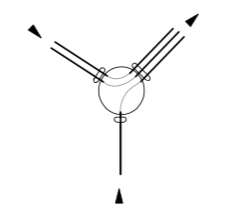
\includegraphics[scale=0.5]{images/intert.png}
    \caption{In this example, $\rho=\rho^1\otimes\rho^{\nicefrac{3}{2}}\otimes\rho^{\nicefrac{1}{2}}\cong\Sym^2\otimes\Sym^3\otimes\Sym^1$.}
\end{figure}

 In the above example with $j_1=1,\,j_2=\frac{3}{2},\,j_3=\frac{1}{2}$, one gets a unique solution (up to permutations) on the form
 $$\begin{cases}
     i_{12}=0\\
     i_{13}=1\\
     i_{23}=2
 \end{cases}$$
where one can observe each $i_{ab}$ to identify intertwiners among the fundamental representations $\rho^{\nicefrac{1}{2}}$ appearing in $\rho^{j_a}$ and $\rho^{j_b}$. This concludes that the ways of intertwine threads correspond to isotropic generators in the support of the product representation.
\end{proof}


\subsubsection{Construction of isotropic basis: some useful examples}

Let us now implement Theorem \ref{intert_isotrop} to find out explicit basis of isotropic subspaces. For that, we have to fix some conventions: let $V$ be the support space of a representation $\rho$, then we can consider the canonical \emph{dual representation} $\rho^*$, which is supported on $V^*$. Even though $V\cong V^*$, the representations $\rho$ and $\rho^*$ cannot be consider as canonically isomorphic as well, since e.g., for a fixed $U\in\SU(2)$,
$$\begin{matrix}
    \rho^{\nicefrac{1}{2}}(U):\C^2\to\C^2\\
    \qquad\qquad\quad e_A\mapsto U_A^Be_B
\end{matrix}\qquad\begin{matrix}
    {\rho^{\nicefrac{1}{2}}}^*(U):{\C^2}^*\to{\C^2}^*\\
    \qquad\qquad\quad e^A\mapsto e^B\overline{U}_B^A
\end{matrix}$$
are quite different representations. Our convention, though, will be $\{e_A\}_{A=1,2}$ spanning $\C^2$ and $\{e^A\}_{A=1,2}$ spanning ${\C^2}^*$, and allows us to give an orientation to our graphs, by associating ${\rho^{\nicefrac{1}{2}}}^*$ and $\rho^{\nicefrac{1}{2}}$ to the outgoing and incoming threads, respectively\footnote{For instance, Figure 3.1 in this convention is representing $\rho^1\otimes{\rho^{\nicefrac{3}{2}}}^*\otimes\rho^{\nicefrac{1}{2}}$.}. This is not an usual choice in literature and it makes all the machinery much clearer; we refer to \cite{LN6}. 

In particular, it imposes precise rules of saturation for indices in the research of an isotropic basis, as we are going to see in no time.

\begin{example}[Isotropic subspaces of product representations]\label{isotr_basis}
In the following, we are discussing some examples isotropic subspaces, pointing out their basis explicitly, even for dual and non--dual factors.
    \begin{itemize}
        \item $\rho^{\nicefrac{1}{2}}\otimes{\rho^{\nicefrac{1}{2}}}^*$ is supported in $\C^2\otimes{\C^2}^*$ spanned by $\{e_A\otimes e^B\}$. An isotropic vector in this space must satisfy, $w=\rho^{\nicefrac{1}{2}}\otimes{\rho^{\nicefrac{1}{2}}}^*(U)[w]$, \emph{i.e.}
        $$w_B^Ae_A\otimes e^B=w_B^AU_A^C\overline{U}_D^B\,e_C\otimes e^D\quad\Leftrightarrow\quad w_B^A=\delta_B^A$$
        hence, there is a $1$--dimensional isotropic subspace $\Inv(\rho)=\spann\{\delta_B^A\,e_A\otimes e^B\}$ of the support space $\C^2\otimes{\C^2}^*$ \emph{(}as well as only $1$ possible way of intertwining $\rho^{\nicefrac{1}{2}}$ and ${\rho^{\nicefrac{1}{2}}}^*$ is there\emph{)}. Notice that, if we had $\rho^{\nicefrac{1}{2}}\otimes\rho^{\nicefrac{1}{2}}$ or ${\rho^{\nicefrac{1}{2}}}^*\otimes{\rho^{\nicefrac{1}{2}}}^*$, we would have got basis spanned by $\{\epsilon^{AB}\,e_A\otimes e_B\}$ or $\{\epsilon_{AB}e^A\otimes e^B\}$, respectively.

        \item Let us discuss $\rho={\rho^1}\otimes{\rho^1}={\rho^{\nicefrac{1}{2}}}\odot{\rho^{\nicefrac{1}{2}}}\otimes{\rho^{\nicefrac{1}{2}}}\odot{\rho^{\nicefrac{1}{2}}}$, represented as a node with  a pair of two ingoing threads. The support of this representation is given by $\C^2\odot\C^2\otimes\C^2\odot\C^2=\spann\{e_{A_1}\odot e_{A_2}\otimes e_{B_1}\odot e_{B_2}\}$ and, also here, only a $1$--dimensional isotropic subspace $\Inv(\rho)$ does exist, spanned by 
        $$w=\epsilon^{A_1B_1}\epsilon^{A_2B_2}\,e_{A_1}\odot e_{A_2}\otimes e_{B_1}\odot e_{B_2}$$

        \item Let us discuss the case $\rho=\rho^{j_1}\otimes\rho^{j_2}\otimes\rho^{j_3}$ supported in $\C^{2j_1+1}\otimes\C^{2j_2+1}\otimes\C^{2j_3+1}$ given in \emph{Figure 3.2}. Here the factors of the support result on the form
        \begin{align*}
            \C^{2j_1+1}&\cong\C^2\odot\C^2\odot\C^2=\spann\bigg\{e_{A_1}\odot e_{A_2}\odot e_{A_3}\bigg\}\\
            \C^{2j_2+1}&\cong{\C^2}^*\odot{\C^2}^*=\spann\bigg\{e^{B_1}\odot e^{B_2}\bigg\}\\
            \C^{2j_3+1}&\cong\C^2\odot\C^2\odot\C^2=\spann\bigg\{e_{C_1}\odot e_{C_2}\odot e_{C_3}\bigg\}
        \end{align*}
      and an isotropic vector for such a representation $\rho$ satisfies
      $$w_{B_1B_2}^{A_1A_2A_3C_1C_2C_3}\,e_{A_1}\odot e_{A_2}\odot e_{A_3}\otimes\ e^{B_1}\odot e^{B_2}\otimes e_{C_1}\odot e_{C_2}\odot e_{C_3}=\rho(U)w$$
      and \emph{Theorem \ref{intert_isotrop}} imposes we must intertwine together indices $(A_1,C_1)$, $(A_2,C_2)$,$\,(B_1,A_3),\, (B_2,C_3)$, yielding again only $1$ isotropic vector, spanning so a $1$--dimensional isotropic subspace $\Inv(\rho)=\spann\{w\}$, where
      $$w=\epsilon^{A_1C_1}\epsilon^{A_2C_2}\delta_{B_1}^{A_3}\delta_{B_2}^{C_3}\,e_{A_1}\odot e_{A_2}\odot e_{A_3}\otimes\ e^{B_1}\odot e^{B_2}\otimes e_{C_1}\odot e_{C_2}\odot e_{C_3}$$

      \begin{figure}[ht]
            \centering
            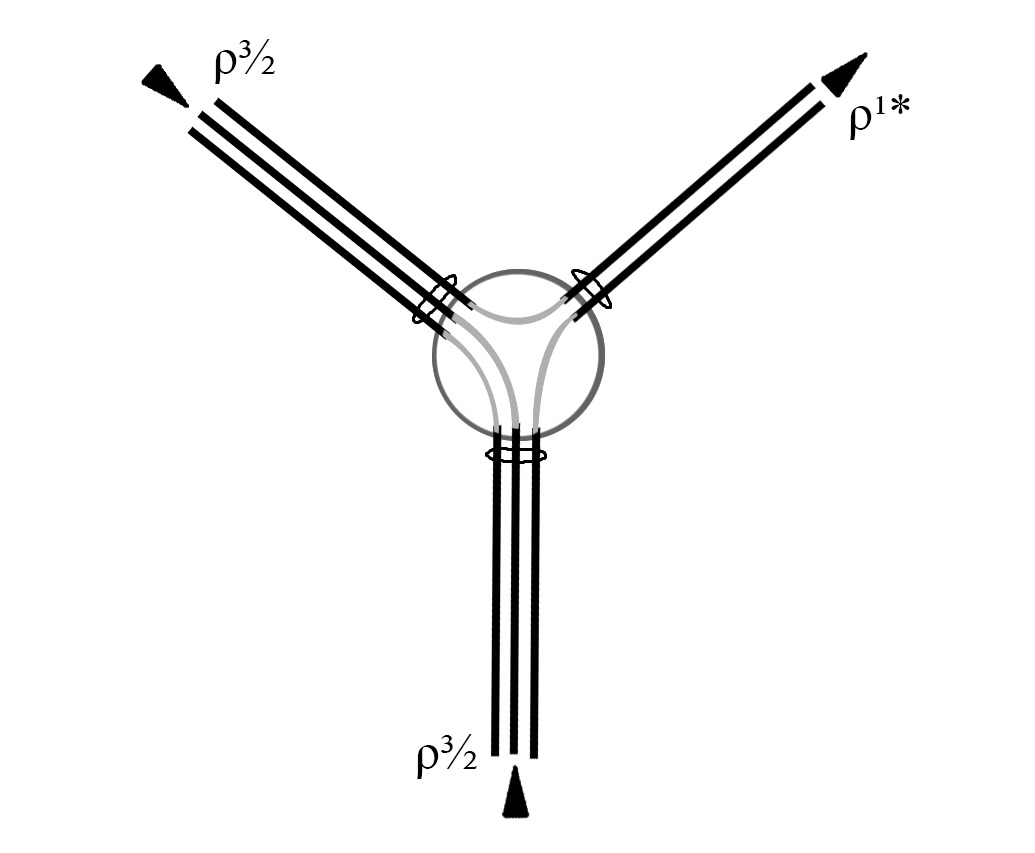
\includegraphics[scale=0.20]{images/intert_j1_j2_j3.jpeg}
            \caption{In this example, $\rho=\Sym^3\otimes{\Sym^2}^*\otimes\Sym^3$.}
        \end{figure}

      %\item Let us finally discuss a case that allows \,$2$--dimensional isotropic subspaces:
      %$$\vdots$$
     
    
    
    


    \item Let us also present a case on which there is no correspondence among intertwiners and independent isotropic vectors. Consider the following
    $$\rho={\rho^{\nicefrac{1}{2}}}^*\otimes\rho^{\nicefrac{1}{2}}\otimes{\rho^{\nicefrac{1}{2}}}^*\otimes\rho^{\nicefrac{1}{2}}$$
    from which one can intertwine the different nodes getting as isotropic vectors 
    \begin{align*}
        v_I&=\delta_A^D\delta_C^B\,e^A\otimes e_B\otimes e^C\otimes e_D\\
        v_{II}&=\delta_A^B\delta_C^D\,e^A\otimes e_B\otimes e^C \otimes e_D\\
        v_{III}&=\epsilon_{AC}\epsilon^{BD}\,e^A\otimes e_B\otimes e^C \otimes e_D
    \end{align*}
    which is clearly non--linear independent generators, since
    \begin{align*}
        v_{III}&=\epsilon_{AC}\epsilon^{BD}\,e^A\otimes e_B\otimes e^C \otimes e_D\\
        &=\left(\delta_A^B\delta_C^D-\delta_C^B\delta_A^D\right)\,e^A\otimes e_B\otimes e^C \otimes e_D\\
        &=v_{II}-v_I
    \end{align*}
    Hence, here is $\dim(\Inv(\rho))=2$ being $\Inv(\rho)$ spanned by only two of $v_j$s.
    \end{itemize}
\end{example}

%Let us conclude this section by defining generators  for the Lie algebra $\su(2)$ satisfying\footnote{They are actually involved in the afore--mentioned classification of the irreducible representations of $\SU(2)$.}
%$$\begin{cases}
 %   [h,h]=0\\
  %  [h,L_{\pm}]=\pm2 L_{\pm}\\
   % [L_+,L_-]=h
%\end{cases}$$
We conclude this section showcasing the Casimir operator of $\su(2)$ defined as
$$\tau^2:=-\sum_{i=1}^3(\tau_i)^2=L_++L_-+\frac{1}{2}h^2$$
for $h:=\sigma_3,\,L_{\pm}:=\frac{1}{2}(\sigma_1\pm\sigma_2)$, being $\sigma_i$ Pauli matrices and $\tau_i:=-\frac{i}{2}\sigma_i$.

{
\begin{remark}\label{Casimir}
Since $\tau^2$ commutes with $h,L_\pm$, then it is a central element of the universal enveloping algebra of $\su(2)$\footnote{Indeed, the universal enveloping algebra of $\su(2)$ is the associative algebra over $\C$ generated by ${h,L_+,L_-}$ satisfying $[L_\pm,L_\pm]=h, [h,L_\pm]=\pm L_\pm$; see Section 5.1 of \cite{kirillov} for these standard definitions. Moreover, by CFR. with Proposition 6.15 of \cite{kirillov}, this Casimir is obtained as associated to the bilinear form on $\su(2)$ defined by $(x,y):=\tr(xy)$.}; in particular, for any representation $\T\rho:\su(2)\to\gl_n$ supported on some vector space $V$, the element $\T\rho(\tau^2):V\to V$ commutes with the action of $\su(2)$ on $V$ and hence it is an intertwiner. Applying \emph{Theorem \ref{shur}} yields $\tau^2$ acting as a constant multiplication, if $\rho=\rho^j$ is some spin representation supported on $V_{n_{(j)}}$, \emph{i.e.} it holds $\T\rho^j(\tau^2)=-j(j+1)\mathbb{1}_{n_{(j)}}$, for any $j\in\frac{1}{2}\N$ such that $n_{(j)}=2j+1$. In particular, $\tau^2$ does not depend on the choice of the basis of $\su(2)$.
\end{remark}
}

%\newpage
%$$\text{see representation, Fatib. pag 704}$$

%$$\mathfrak{diffeo}(\M)\cong\Der(\M)$$



\subsubsection{About the Haar measure on \texorpdfstring{$\SU(2)$}{a}}
The Haar measure perfectly fits with the background--free essence of LQG, being in fact a well--defined canonical object in any compact Lie group and it is the main reason why it was originally essential to find compact reduction of the non--compact group $\SL(2,\C)$. %Although A. Weil and H. Cartan proved the general result
We refer to Section 4.6 of \cite{kirillov} for the general result
\begin{teo}[Haar]
    Let $\G$ be a compact real Lie group, then it supports a canonical Borel measure $\d\g$ which is both left and right--invariant and also invariant under $\g\mapsto\g^{-1}$ and which satisfies $\int_\G\d\g=1$. This measure is called the \emph{Haar measure} on $\G$ and is usually denoted by $\d\g$.
\end{teo}

Although it is of astonishing important to give the fully characterisation of finite--dimensional representation of compact Lie groups as unitary, hence, completely reducible, we shall discuss the Haar measure only in our case of interest 
$$\G=\SU(2)=\left\{\begin{bmatrix}
    u&v\\
    -\overline{v}&\overline{u}
\end{bmatrix}:\,u,v\in\C,\,|u|^2+|v|^2=1\right\}\cong\S^3\subseteq\C^2\subseteq\mathbb{H}$$
where the quaternions are defined as---for $\mathbf{i}^2=\mathbf{j}^2=\mathbf{k}^2=\mathbf{i}\mathbf{j}\mathbf{k}=-1$
$$\mathbb{H}=:\{a\mathbb{I}+b\mathbf{i}+c\mathbf{j}+d\mathbf{k}\,|\,a,b,c,d\in\R\}\cong\R^4$$
This way, it can be shown, e.g. by using Clifford algebras, that the following characterisation holds true
$$\SU(2)=\{U\in\mathbb{H}\,|\,a^2+b^2+c^2+d^2=1\}$$
and we can define a metric on $\SU(2)$ by pulling--back along the embedding $\S^3\hookrightarrow(\R^4,\delta)$.\, For that,
being $\su(2)\cong T_{\mathbb{I}}\S^3\cong\R^3$, we can use stereographic coordinates in $\R^3$, given by $(x,y,z)=\frac{1}{1+a}\left(b,c,d\right)$, to cover $\SU(2)\setminus\{-\mathbb{1}\}$. Hence, we read the embedding as---for $v\in\R^3$ such that $|v|^2=x^2+y^2+z^2$
$$\begin{matrix}
    \imath:\SU(2)\to\mathbb{H}\\
   \qquad\qquad(x,y,z)\mapsto\frac{1}{1+|v|^2}\bigg(1-|v|^2,2x,2y,2z\bigg)
\end{matrix}$$
Then, the Haar metric on $\SU(2)$ turns out to be
\begin{align*}
    g_{\SU(2)}&=\imath^*\delta=\imath^*\left(\d a^2+\d b^2+\d c^2+\d d^2\right)=\frac{2^4}{(1+|v|^2)^2}\left(\d x^2+\d y^2+\d z^2\right)
\end{align*}
which induces the \emph{Haar measure} on measurable functions $f:\SU(2)\to\R$
$$\int_{\SU(2)}f(U)\,\d U=\frac{4}{\pi}\int_{\R^3}f(U(v))\frac{\d v}{(1+|v|^2)^3}$$
Here the volume of $\SU(2)$ is finite and such a measure is left and right invariant (inherited by the fact that $\S^3$ is rotationally invariant) and it is normalized by
$$\int_{\SU(2)}\d U=1$$

%E' fondamentle dire qui che la metrica di Haar è pefetta per lavorare in background--free perchè permetterà poi di definire un prodotto interno su uno spazio di Hilbert che non è una metrica Einstein--like, già fissata su una $(\M^\eta,g)$! Dipende solo dalla natura "gruppale" della varietà $\SU(2)$ e non si fissa una metrica a--priori. Però $\SU(2)$ è compatto despite $\SL(2,\C)$




\subsection{Hilbert spaces of quantum states}

%$$\mathcal{H}\,\text{Hilbert è separabile iff ha una base ortonormale numerabile}$$
%\,\newline
At long last, we are ready to construct the quantum phase space of the theory. As widely discussed in the previous, kinematic quantum states of LQG shall be represented by functionals of a $\SU(2)$--discrete gauge connection, hence they should close within a Hilbert space of the form
$$\mathcal{H}_\Gamma:=L_2\bigg[\nicefrac{\SU(2)^\Latt}{\SU(2)^N}\bigg]$$
%defines a non--separable Hilbert?\, Seeking for some separable space, we go through discretized connections. (mhmm chiedi)\\
We saw a discrete connection being represented by a lattice $\Gamma=(N,\Latt)$ on which a group element $\h(\A,\gamma)$ is attached at each link, defining a so--called discrete structure. Accordingly, a discrete connection is a map $\h:\Latt\to\SU(2)$ or, equivalently, a point in $\{\h_\gamma\}_{\gamma\in\Latt}\in\SU(2)^\Latt$. A discrete version of fucntionals $\Psi[\A]$ will be so given by an element in the (infinite--dimensional) $\C$--vector space
$$\bigg\{\Psi:\SU(2)^\Latt\to\C\bigg\}=:\Kk_\Gamma$$
%i.e. $\Psi[U]$, for some $U_\gamma\in\SU(2)$.\, 
Being the set of all lattices $\{\Gamma_k\}_{k\in\mathcal{I}}$ a direct family, we now would want to endow $\{\Kk_{\Gamma_k}\}_{k\in\mathcal{I}}$ with the same direct structure.

\begin{defi}[Cylindric functional]
    Let $(\Gamma,\h)$ be a discrete structure on $\Sigma$ and consider a smooth function $f:\SU(2)^\Latt\to\C$, then we define
    $$\begin{matrix}
        \psi_{\Gamma,f}:\SU(2)^\Latt\to\C\\
        \qquad\qquad\qquad\qquad(\h_\gamma)_{\gamma\in\Latt}\mapsto f(\h_{\gamma_1},\hdots,\h_{\gamma_{\#\Latt}})
    \end{matrix}$$
    to be the \emph{cylindric functional} generated by the lattice $\Gamma$ and the $\SU(2)$--discrete connection $\h$ through $f$. The space of all cylindric functionals on a lattice $\Gamma$ is denoted by $\Kk_\Gamma$ too.
\end{defi}

\begin{note}
    From now on, for the sake of nimbleness, we will write cylindrical functionals as $\psi_{\Gamma,f}(\h)=f(\h_1,\hdots,\h_\Latt)$, or $\psi_{\Gamma,f}(U)=f(U_1,\hdots,U_\Latt)$, with an abuse of notation on $\Latt$.
\end{note}

By considering two lattices $\Gamma_k\hookrightarrow\Gamma_h$ we can can embed links of the less fine in the finer one as $\imath_k^h:\Latt_k\to\Latt_h$, which defines the projection map---for $\h_h:\Latt_h\to\SU(2)$\footnote{Notice that it simply forgets the group elements on the links of the finer $\Gamma_h$ which are not links of the less fine $\Gamma_k$, leaving
the others unchanged.}
$$\begin{matrix}
    p_k^h:\SU(2)^{\Latt_h}\to\SU(2)^{\Latt_k}\\
    \qquad\h_h\mapsto\h_h\circ\imath_k^h
\end{matrix}$$
This way, it comes natural to extend cylindric functionals $\psi_{\Gamma_k,f_k}$ to the finer lattice $\Gamma_h$:\, first, we define new functions $f_h:=f_k\circ p^h_k:\SU(2)^{\Latt_h}\to\C$ to be constant along the links in $\Gamma_h$ which do not lie in $\Gamma_k$, so that the map

$$\begin{matrix}
    \iota_k^h:\Kk_{\Gamma_k}\to\Kk_{\Gamma_h}\\
    \quad\psi_{\Gamma_k,f_k}\mapsto\psi_{\Gamma_h,f_h}
\end{matrix}$$
carries the partial ordered structure of the family of lattices to the family of functionals ${\{\Kk_{\Gamma_k}\}}_k$. Thereafter, there exists an upper bound $\Kk_\Gamma$ refining both $\Kk_{\Gamma_k},\Kk_{\Gamma_h}$ for each $k,h$, which defines a \emph{direct limit} $\Kk$ together with a family of linear maps $\iota_k:\Kk_{\Gamma_k}\to\Kk$ obeying to the following universal property: \emph{for any vector space $V$ where a family of linear maps $\lambda_k:\Kk_{\Gamma_k}\to V$ satisfying $\Gamma_k\hookrightarrow\Gamma_h\,\Rightarrow\,\lambda_k=\lambda_h\circ\iota_k^h$ is given, there exists a unique map $\lambda:\Kk\to V$ such that $\lambda_k=\lambda\circ\iota_k$.}\\

    As it is usual for universal properties, it can be shown that the direct limit $(\Kk,\iota_k)$ is unique up to isomorphisms;\, moreover, it turns out that functionals $\psi\in\Kk$ are on the form $\psi=\psi_{\Gamma_k,f_k}$, for a finite lattice $\Gamma_k$ and and a function $f_k$ such that $\psi_{\Gamma_k,f_k}$ is cylindric. Eventually, $\psi=\iota^h_k(\psi_{\Gamma_k,f_k})$ whenever a finer lattice $\Gamma_h\hookleftarrow\Gamma_k$ is there.%\footnote{CFR polynomials}

All the above allows us to go through the following argument: let $\psi_{\Gamma_k,f_k},\psi_{\Gamma_h,f_h}$ be two cylindrical functionals, then they can be regarded as $\iota_k^j(\psi_{\Gamma_k,f_h}), \iota^j_h(\psi_{\Gamma_h,f_h})\in\Kk_{\Gamma_j}$ respectively, once $\Gamma_j$ refines both $\Gamma_k$ and $\Gamma_h$, and one can define a bilinear map $\langle\cdot,\cdot\rangle:\Kk_j\times\Kk_j\to\C$ on the refinement as---said $\d U_1\hdots\d U_\Latt=:\d\mathcal{U}$ the Haar measure on $\Latt$ copies of $\SU(2)$, which is still a compact real Lie group
\begin{equation}\label{inner_pr}
\bigg\langle\psi_{\Gamma_k,f_k},\psi_{\Gamma_h,f_h}\bigg\rangle:=\int_{\SU(2)^\Latt}\overline{f_k(U_1,\hdots,U_\Latt)}f_h(U_1,\hdots,U_\Latt)\,\d U_1\hdots\d U_\Latt
\end{equation}
which extends to the direct limit $\Kk$. This way, one could prove the following
\begin{teo}[Hilbert space of kinematical states]
    $${\Kk'}_\Gamma:=L_2\bigg(\SU(2)^\Latt,\d\mathcal{U}\bigg)=\bigg\{\psi\in\Kk_\Gamma\,\bigg|\,\langle\psi,\psi\rangle<\infty\bigg\}$$
    is a Hilbert space with inner product defined by \emph{(\ref{inner_pr})} on a refinement $\Gamma$.
\end{teo}
\,\newline
Said $\mathbb{K}$ the Hilbert space of linear continuous functionals $\Kk\to\C$, then the triple $\Kk\subset\Kk'\subset\mathbb{K}$ identifies the rigged Hilbert space of kinematic states\footnote{In the jargon of algebraic QFT, it is a so--called \emph{Gelfand triple}, see Section 8.3 of \cite{moretti}.}.\\

We can now deepen in on such a Hilbert space of functionals of discrete $\SU(2)$--connections by involving the spin representations $\rho^{j}:\SU(2)\to\GL(\C^{2j+1})$, well discussed along the whole previous Section 3.1.2, in order to find out some basis. 

The whole machinery is based on the fundamental 

{\begin{teo}[Peter--Weyl]\label{peter_weyl}
    Let $\G$ be a compact Lie group and suppose there exists a \emph{(}unitary\emph{)} $n$--dimensional irreducible representation $\rho:\G\to\End(V)$. Writing the operator $\rho(\g):V\to V$ in a given basis of $V$ yields $\rho$ as a $\GL_n$--valued function on $\G$ having entries $\rho^\alpha_\beta$ being in turn scalar--valued functions on $\G$, for $\alpha,\beta=1,\hdots,n$, \emph{i.e.}
    $$\begin{matrix}
        \rho^\alpha_\beta:\G\to\C\\
        \qquad\qquad\g\mapsto\rho^\alpha_\beta(\g)
    \end{matrix}$$
    Then, it holds $\rho^\alpha_\beta\in L_2(\G,\d\g)$. Moreover, any two such functions are orthogonal with norm squared $\int_\G\rho^\alpha_\beta(\g)\overline{\rho^\mu_\nu(\g)}\,\d\g=\delta^\alpha_\beta\delta^\mu_\nu/{n}$, with respect to the natural inner product on $\Cinf(\G,\C)$ induced by the Haar measure $\d\g$.
    \end{teo}}
    %if $\rho_V,\rho_W:\G\to V,W$ are two non--isomorphic irreducible representations of $\G$, then it holds
    %$$\bigg(\rho_{\alpha\beta}^V(\g),\rho_{ab}^W(\g)\bigg)=0$$
    %for any $\alpha,\beta,a,b=1,\hdots,n$, where $(\cdot,\cdot)$ is the inner product on $\Cinf(\G,\C)$ induced by $\d\g$.
    

    
    %Then, it holds $\ket{j;^\alpha,_\beta}\in L_2(\G,\d\g)$ where $\d\g$ is the Haar measure of $\G$ and
    %$$\begin{matrix}
    %\ket{j;^\alpha,_\beta}:\G\to\C\\
    %\qquad\qquad\qquad \g\mapsto{\rho^{(j)}(\g)}^\alpha_\beta
    %\end{matrix}$$
 

{\begin{proof}
    See Section 4.7 of \cite{kirillov}.
\end{proof}}

{Peter--Weyl theorem applies to $\SU(2)$, where unitary irreducible representations are the spin ones $\rho^j$ being matricially represented by entries which are complex--valued functions on $\SU(2)$ of the form---in the standard notation of \cite{rov1}}
{
$$\begin{matrix}
    \ket{j;^\alpha,_\beta}:\SU(2)\to\C\\
    \qquad\qquad\qquad U\mapsto{\rho^{(j)}(U)}^\alpha_\beta
\end{matrix}$$}
{and the theorem assures $\ket{j;^\alpha,_\beta}\in L_2(\SU(2),\d U)$, where indices $\alpha,\beta=-j,\hdots,j$ move by $2j+1$ integer steps. This naturally extends to $\Kk'_\Gamma$, being $\SU(2)^\Latt$ still compact, yielding}
{$$\begin{matrix}
    \ket{\Gamma;j_\Latt;^{\alpha_\Latt},_{\beta_{\Latt}}}:\overbrace{\SU(2)\times\hdots\times\SU(2)}^{\Latt\text{--times}}\to\C\\
    \qquad\qquad\qquad\qquad\qquad\qquad\qquad\qquad (U_1,\hdots,U_\Latt)\mapsto\rho^{(j_1)}(U_1)^{\alpha_1}_{\beta_1}\hdots\rho^{(j_\Latt)}(U_\Latt)^{\alpha_\Latt}_{\beta_\Latt}
\end{matrix}$$}
{to be an orthonormal basis of ${\Kk'}_\Gamma$, so--called \emph{Peter--Weyl basis}. This way, a general state $\ket{\psi}\in{\Kk'}_\Gamma$ writes as the linear combination---in Einstein sum convention on the matrix indices
$$\ket{\Gamma;j_\Latt}:=\left(\prod_{n\in N}c^{\beta_{i_1}\hdots\beta_{i_t}}_{\alpha_{j_1}\hdots\alpha_{j_o}}\right)\ket{\Gamma;j_\Latt;^{\alpha_\Latt},_{\beta_{\Latt}}}\in{\Kk'}_\Gamma$$
where coefficients $c^{\beta_{i_1}\hdots\beta_{i_t}}_{\alpha_{j_1}\hdots\alpha_{j_o}}$ are there to saturate the combination at each node $n$, where $(\gamma_{i_1},\hdots,\gamma_{i_t})$ incoming and $(\gamma_{j_1},\hdots,\gamma_{j_o})$ outgoing links are there. }

{Notice that, since the spin representations are labelled by semi--integer colours $j$, we have just provided ${\Kk'}_\Gamma$ with a countable basis $\{\ket{\Gamma;j}\}_{j}$, hence it is a separable Hilbert space. }

{Unfortunately, since we get the quantum phase space $\Kk'$ by direct limit, we would expect the union of $\{\ket{\Gamma,j}\}_j$ over all possibles (uncountables) $\Gamma\in\boldsymbol{\Gamma}$ to provide such a basis, but this cannot be countable, hence $\Kk'$ cannot be separable\footnote{{Despite not being separable is an issue by its own for a Hilbert states' space of a quantum theory (see Section \ref{first_quantisation}), one has here to avoid another problem: when we go through direct limit from $\Kk'_\Gamma$ to $\Kk'$, since the embeddings $\iota^h_k$ are constant on the new links in the finer lattice, they are labelled by the trivial representation $\rho^0$. This produces an over--counting in the union and it is for this reason that we restrict the spin representations to be labelled by $j\neq0$, i.e. $\cup_{\Gamma\in\boldsymbol{\Gamma}}\{\ket{\Gamma,j_\Latt}\}_{j\neq0}$ identifies a basis of $\Kk'$.}}.}

%one gets $\ket{\psi_\Gamma}=c_{j_\Latt}\ket{\Gamma,j_\Latt}$ for a general vector in ${\Kk'}_\Gamma$ expressed in the Peter--Weyl basis. %$\{\ket{\Gamma,j_\Latt}\}_j$.\, 

%Notice that, since such a Hilbert space underlies finite lattices in the functional space $\boldsymbol{\Gamma}$, the Peter--Weyl theorem imposes we get an orthogonal functional for any (even slightly) deformation of a link in a lattice, i.e. the basis $\{\ket{\Gamma;j_\Latt}\}_j$ is uncountable, hence ${\Kk'}_\Gamma$ is not separable. 

%\begin{example}
   % $\C^2\otimes\C^2=\spann\{\ket{+,+},\ket{+,-},\ket{-,+},\ket{-,-}\}$
%\end{example}

\begin{remark}
    As a matter of fact, we can represent the states $\ket{\Gamma;j_\Latt;^{\alpha_\Latt},_{\beta_\Latt}}$ graphically by drawing the lattice $\Gamma$, labelling each link $\gamma_k$ by its spin $j_k$ and noting the index $\alpha_k$ at the origin of the link and $\beta_k$ at its target.\, Besides, this notation is consistent with the action of gauge--transformations we discussed in \emph{Section \ref{repr_su}}. %Of course, this graphic representation only strands for the functional associated to the state.
\end{remark}

%\subsubsection{Interlude: Lie operators and (multi) loop states}
%For later convenience, we introduce here Lie operators and (multi) loop states as we will use later and also because of their historical importance, having been introduced since the first attempts of describing LQG.



Consider now a loop $\alpha=\gamma_1*\gamma_2$ with holonomy $\h(\A,\alpha)=\h(\A,\gamma_1)\cdot\h(\A,\gamma_2)$, then the trace operator $\tr:\SU(2)\to\C$ turns out to be a cylindric functional which allows to give the following

\begin{defi}[Loop states]
    Let $\alpha=\gamma_1*\gamma_2$ be a loop on a given discrete structure $(\Gamma,\A)$. A \emph{loop state} is defined as
    $$\Phi_\alpha[\A]:=\tr(\h(\A,\alpha))=\tr\bigg(\h(\A,\gamma_1)\cdot\h(\A,\gamma_2)\bigg)$$
    Analogously, a finite family of loop $\boldsymbol{\alpha}=(\alpha_1,\hdots,\alpha_\Latt)$ define a \emph{multi--loop state} 
$$\Phi_{\boldsymbol{\alpha}}[\A]:=\Phi_{\alpha_1}[\A]\hdots\Phi_{\alpha_\Latt}[\A]$$
\end{defi}
\,\newline
They will turn out to be generators of gauge--invariant states and it will be observed that an invariant gauge--state writes as a combination of multi--loops, ruling out parallel transports from the theory, just allowing holonomies of loops. Moreover, they are normalized by
$$|\Phi_\alpha|^2=\int_{\SU(2)}|\tr(U)|^2\,\d U=1$$
and also allow to construct loop functionals out of loop states via the so--called \emph{loop transform} $\Psi[\alpha]:=\langle{\Phi_\alpha}|{\Psi}\rangle$ of a quantum state $\ket{\Psi}$.

Now we can implement the covariance of the theory to single out the invariant, covariant and eventually physical states.

\subsubsection{Gauge--covariant states}
It is easily checked that gauge--invariant functionals on the lattice $\Gamma$ do restrict to a closed subspace ${\Gg'}_\Gamma\subseteq{\Kk'}_\Gamma$, hence the inner product (\ref{inner_pr}) is inherited. As for generic kinematical states, also in ${\Gg'}_\Gamma$ we have the dense subspace $\Gg_\Gamma$ of smooth gauge invariant states which, by direct limit on the lattices, defines the rigged Hilbert space---said $\mathbb{G}$ the space of gauge--invariant distribution states
$$\Gg'\subset{\Gg}\subset\mathbb{G}$$
\,\newline
Let us now look for some basis of $\Gg'$:\, being Peter--Weyl states defined through products of irreducible representations of $\SU(2)$, the whole powerful graphical calculus developed in Section \ref{repr_su} directly applies and, as already said, it turns out that states $\Psi[\A]$ are exactly represented by holonomies of the discrete connection, hence, by loops\footnote{That is the reason why we refer to the theory as Loop Quantum Gravity.}. For the sake of simplicity, let us discuss the case of Figure 3.3, where a Peter--Weyl state in ${\Kk'}_\Gamma$ here comes in the form%\footnote{Notice that a Peter--Weyl state is a product representation of $\SU(2)$, well understood.}
$$\psi(U_1,U_2)=c^{\beta_1\beta_2}_{\alpha_1\alpha_2}\,\rho^{(j_1)}(U_1)^{\alpha_1}_{\beta_1}\rho^{(j_2)}(U_2)^{\alpha_2}_{\beta_2}$$
and a gauge--transformation $\Phi\in\mathscr{G}$ restricts to a discretized gauge--map $\varphi\in\SU(2)^N$ acting in either dual or non--dual representation on each node, depending on the orientation of the leaving link, i.e. it holds
$$\Phi_*\psi(U_1,U_2)=\overbrace{\rho^*_{(j_1)}(\overline{\varphi})^{{\alpha_1}'}_{\alpha_1}\rho^{(j_1)}(\varphi)^{\beta_1}_{{\beta_1}'}\,c^{{\beta_1}'{\beta_2}'}_{{\alpha_1}'{\alpha_2}'}\,\rho^*_{(j_2)}(\overline{\varphi})^{{\alpha_2}'}_{\alpha_2}\rho^{(j_2)}(\varphi)^{\beta_2}_{{\beta_2}'}}^{=:{c'}^{\beta_1\beta_2}_{\alpha_1\alpha_2}=\varphi\cdot c}{\rho'}^{(j_1)}(U_1)^{\alpha_1}_{\beta_1}{\rho'}^{(j_2)}(U_2)^{\alpha_2}_{\beta_2}$$

\begin{figure}[ht]
    \centering
    \begin{tikzpicture}
    \draw[dashed] (0,0) circle (.3);

    \fill (.3*.707, .3*.707) circle (.05)
          (.3*.707, -.3*.707) circle (.05)
          (-.3*.707, .3*.707) circle (.05)
          (-.3*.707, -.3*.707) circle (.05);
          %(0,2.18) circle (.05)
          %(0,-2.18) circle (.05);

    \draw[->] plot coordinates {(-.1,2.18) (0,2.18)};
    \draw[smooth] plot coordinates {(-.3*.707,.3*.707) (-.707, 2) (.707, 2) (.3*.707,.3*.707)};

    \draw[smooth] plot coordinates {(-.3*.707,-.3*.707) (-.707, -2) (.707, -2) (.3*.707, -.3*.707)};
    \draw[<-] plot coordinates {(-.1,-2.18) (0,-2.18)};

    \draw (1,1.3) circle (0) node {$\gamma_1$};
    \draw (-1,-1.3) circle (0) node {$\gamma_2$};
\end{tikzpicture}
    \caption{This draw relies on the graphical representation discussed in Section \ref{repr_su}. The dashed ball models the product representation carried by the Peter--Weyl state, each link represents the product factor and labels with $\alpha_i,\beta_i$ the linking nodes, on which the correspondent discretized gauge map is acting.}
\end{figure}
\,\newline
This shows that a functional in ${\Kk'}_\Gamma$ is not gauge--invariant, in general, but also, underscores that gauge--invariance $\Phi_*\psi=\psi$ is fulfilled for ${c'}^{\beta_1\beta_2}_{\alpha_1\alpha_2}=c^{\beta_1\beta_2}_{\alpha_1\alpha_2}$ {(i.e. $\varphi\cdot c=c$)} or, in the jargon of representations, coefficients $c$ must intertwine the spins ${j_i}$s. In other words, gauge--invariant states correspond to generators of isotropic subspaces of the product representation underlay by the Peter--Weyl basis.

By Theorem \ref{intert_isotrop} and by also arguing as in Example \ref{isotr_basis}, we infer that Figure 3.3 allows intertwiners among the representations of the two holonomies, corresponding to a $2$--dimensional isotropic subspace of the Peter--Weyl underlying representation, showing that multi--loop states are not independent
\begin{align*}
    \psi_I(U_\alpha,U_\beta)&=\rho^{\nicefrac{1}{2}}(U_\alpha)^A_B\,\rho^{\nicefrac{1}{2}}(U_\beta)^C_D\,\delta^B_A\delta^D_C\\
    &=\rho^{\nicefrac{1}{2}}(U_\alpha)^A_A\,\rho^{\nicefrac{1}{2}}(U_\beta)^C_C=\tr(U_\alpha)\tr(U_\beta)
\end{align*}
\begin{align*}
    \psi_{II}(U_\alpha,U_\beta)&=\rho^{\nicefrac{1}{2}}(U_\alpha)^A_B\,\rho^{\nicefrac{1}{2}}(U_\beta)^C_D\,\delta^D_A\delta^B_C\\
    &=\rho^{\nicefrac{1}{2}}(U_\alpha)^D_B\,\rho^{\nicefrac{1}{2}}(U_\beta)^B_D=\tr(U_\alpha\cdot U_\beta)
\end{align*}
\begin{align*}
    \psi_{III}(U_\alpha,U_\beta)&=\rho^{\nicefrac{1}{2}}(U_\alpha)^A_B\,\rho^{\nicefrac{1}{2}}(U_\beta)^C_D\,\epsilon^{BD}\epsilon_{AC}\\
    &=\rho^{\nicefrac{1}{2}}(U_\alpha)^A_B\,\rho^{\nicefrac{1}{2}}(\overline{U_\beta})^B_D=\tr(U_\alpha\cdot\overline{U_\beta})
\end{align*}
\,\newline
 Indeed, Example \ref{isotr_basis} here gives $\psi_{II}-\psi_I+\psi_{III}=0$, represented in the following

\begin{figure}[ht]
    \centering
    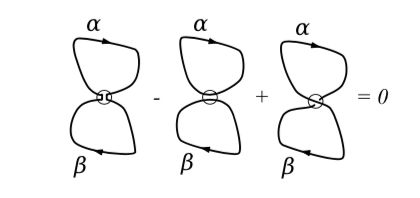
\includegraphics[scale=0.6]{images/multiloops.png}
\end{figure}
 
 \,\newline
 Farther, we got the following Proposition--Definition
\begin{defi}[Spin networks]
    For a lattice $\Gamma$, if a non--trivial spin representation $\rho^{(j)}$ on each link is given, together with an intertwiner on each node, then there exists a unique state in ${\Gg'}_\Gamma$ completely identified by the theory of irreducible representations of $\SU(2)$. We denote such state by $\ket{\Gamma;j_\Latt;i_N}$ and we call it a \emph{spin network}.
\end{defi}
It is worth observing here that
\begin{remark}[Spin networks basis]
    Choosing an independent set of intertwiners rules the ways of linking the different nodes and it also labels them. Thus, if one starts at a node and walks along a leaving line, it will be intertwined with a new node, forming a link which, soon or later, being the lattice finite, will close down to a \emph{(}possibly multi\emph{)} loop. Accordingly, spin networks are independent gauge--invariant multi--loop states, hence they form a \emph{(}still\emph{)} uncountable basis of $\Gg'$, though in ${\Gg'}_\Gamma$ they are countable.
\end{remark}


\subsubsection{\texorpdfstring{$\Diffeo(\Sigma)$}{a}--covariant states}
We now have to solve the diffeomorphism constraint equation for states, imposing $\Diffeo(\Sigma)$--invariance on spin networks. Unfortunately, one readily faces a hitch: by Peter--Weyl Theorem \ref{peter_weyl}, a diffeomorphism of the manifold maps a spin network in an orthogonal one, being affected even by slightly deformations of the $\Sigma$--embedded lattices they are associated with. Moreover, spin networks come with a precise orientation and ordering of the links, which are not left unchanged by the group $\Diffeo(\Sigma)$, in general (see Section 6.4 \cite{rov1}). For this reason, one has to deal with extended diffeomorphisms


\begin{defi}[Extended diffeomorphisms]
    A homeomorphism $\phi:\Sigma\to\Sigma$ of a smooth manifold such that it is a diffeomorphism on a finite number of points is said to be an \emph{extended diffeomorphism} and it writes $\phi\in\Diffeo_*(\Sigma)$.
\end{defi}
\,\newline
The action of $\Diffeo_*(\Sigma)$ can be now quotiented out from ${\Gg'}$ through the following argument: a given extended diffeo $\phi$ drags spin networks in spin networks, for which we write $\phi_*\ket{\Gamma;j_\Latt;i_\Latt}=\ket{\phi(\Gamma);j_\Latt;i_\Latt}$ and one can extend the left action to distributions $\Psi:\Gg\to\C$ in $\mathbb{G}$. For that, define the distribution
$$\begin{matrix}
    \phi^*\Psi:\Gg\to\C\\
    \quad\qquad\qquad\ket{S}\mapsto\Psi(\phi_*\ket{S})
\end{matrix}$$
on test--spin networks, from which one can ask $\Diffeo_*(\Sigma)$--invariance is addressed by states $\ket{S}\in\Gg$ satisfying the equation

\begin{equation}\label{diff_inv_states}
 (\phi^*\Psi)\ket{S}=\Psi\ket{S}   
\end{equation}
This yields a well--defined subspace of spin network functionals $\Psi\in\mathbb{D}\subseteq\mathbb{G}$ satisfying (\ref{diff_inv_states}), for any $\phi\in\Diffeo_*(\Sigma)$ and $\ket{S}\in\Gg$, and allows compatibility with the equivalence relation induced by $\ket{S}\sim\phi_*\ket{S}$ on $\Gg$, defining $\D:=\nicefrac{\Gg}{\sim}$. Moreover, it holds

\begin{teo}[Existence of $\Diffeo_*(\Sigma)$--invariant states]
    There exists a \emph{(}separable\emph{)} subspace $\D'$ of $\Gg'$ made of $\SU(2)$ and $\Diffeo_*(\Sigma)$ invariant kinematical states.
\end{teo}
\begin{proof}[Idea of the proof]
    Consider a gauge--invariant state on the form $\Psi_S\in\Gg$ and let $p(\Psi_S):\Gg\to\C$ be the linear map
    $$p(\Psi_S)\Psi_{S'}=\sum_{\Psi=\phi_*\Psi_S}\langle\Psi,\Psi_{S'}\rangle$$
    for $\phi\in\Diffeo_*(\Sigma)$. In order to prove continuity we claim the sum being finite. Let us expand $\Psi_S,\Psi_{S'}$ in the spin networks basis and take advantage of their graphical representations. Computing $\phi_*\ket{S}$ affects the sum in two possible ways: either the transformed graph is the same of $\ket{S'}$ or it is not. In the former, they must differ by a necessarily finite number of choice representations on each loop, while in the latter they have to be orthogonal states, hence there is no contribution to the sum. Furthermore, the state $p(\Psi_S)\in\mathbb{G}$ is $\Diffeo_*(\Sigma)$--invariant, since
    \begin{align*}
        \phi^*p(\Psi_S)\,\Psi_{S'}&=p(\Psi_S)\phi_*\Psi_{S'}=\sum_{\Psi={\phi'}_*\Psi_S}\langle\Psi,\phi_*\Psi_{S'}\rangle\\
        &=\sum_{\overline{\phi}_*\Psi=\overline{\phi}\circ{\phi'}_*\Psi_S}\langle\overline{\phi}_*\Psi,\Psi_{S'}\rangle=p(\Psi_S)\Psi_{S'}
    \end{align*}
    The above extends from spin networks to the whole $\Gg$ by linearity, yielding $p:\Gg\to\mathbb{D}\subseteq\mathbb{G}$ to be a projection to the quotient $\nicefrac{\Gg}{\sim}$ induced by $\ket{S}\sim\phi_*\ket{S}$. Once such a $p$ is well--defined, an inner product $(\cdot,\cdot):\mathbb{D}\times\mathbb{D}\to\C$ is well--defined by
\begin{equation}
    \bigg(p(\Psi_S),p(\Psi_{S'})\bigg):=p(\Psi_S)(\Psi_{S'})=\sum_{\phi\in\Diffeo_*(\Sigma)}\langle\phi_*\Psi_S,\Psi_{S'}\rangle
\end{equation}
and it induces the rigged Hilbert space $\D\subset{\D}'\subset\mathbb{D}$.
\end{proof}
We just got the following Proposition--Definition

\begin{defi}[Spin knots]
    A \emph{spin knot} is defined to be a basis for $\D'$, hence a $\Diffeo_*(\Sigma)$--invariant spin network, \emph{i.e.} it is a kinematical state satisfying both the gauge and the natural symmetries of Holst theory expressed in equation \emph{(\ref{constr_eqs_psi})}, at a quantum level.
\end{defi}

The whole above construction yields spin knots to be equivalence classes of spin networks, up to extended diffeomorphisms;\, it is not a subset of spin networks in $\Gg'$ with an additional property. In other words, we have to expect the space of spin networks to project onto the space of spin knots, not to be embedded into it\footnote{A final note on the separability of $\D'$. As a consequence of Theorem 3.1.7 and Definition 3.1.10, since the sum in (3.3) is finite, spin knots form a countable basis for $\D'$, which then turns out to be a separable Hilbert space of quantum states. Eventually, the non--separability of $\Gg'$ turns out to be just a gauge artifact---see Section 6.4.2 of \cite{rov1}.}. 

%\begin{remark}[Separability of $\D'$]
 %   As a consequence of \emph{Theorem 3.1.7} and \emph{Definition 3.1.10}, since the sum in \emph{(3.3)} is finite, spin knots form a countable basis for $\D'$, which then turns out to be a separable Hilbert space of quantum states. Eventually, the non--separability of $\Gg'$ turns out to be just a gauge artifact $($see \emph{Section 6.4.2} of \emph{\cite{rov1}}\emph{)}.
%\end{remark}

%As a final...
%$$\vdots$$
%$$\text{\textcolor{red}{Concludi sottolineando $\D'_\Gamma$ separabile e che a questo livello conta solo $\Gamma$ astratto}}$$
%$$\text{\textcolor{red}{aggiungendo che questo non è il vero $\mathcal{H}_{\text{phys}}$ which}}$$
%$$\text{\textcolor{red}{should contain spin foams, as mentioned in...}}$$
%$$\text{\textcolor{red}{vd anche "Reloading Hilbert spaces}}$$

\newpage
\subsection{Invariant operators among \texorpdfstring{$\mathcal{H}_\Gamma$}{a}}
Once a separable Hilbert space $\mathcal{H}_\Gamma$ is there for quantum invariant states, one proceeds to find out well--defined operators in $\Aut(\mathcal{H}_\Gamma)$, looking for the algebra of observables of the gravitational field. It has to be noticed that the operators which matter here would be the ones defined on spin knots or, at least, on spin networks, which then should be $\Diffeo_*(\Sigma)$--quotiented.\, By the way, two non--invariant operators, which will turn out to be related with gauge--connections, arise quite naturally.

We have already got a glimpse of how a Lie algebra element $\theta^i\tau_i\in\su(2)$ acts on a product state, by acting once at each link at a node. For instance, in a product representation $\rho^{j_1}\otimes\rho^{j_2}\otimes\rho^{j_3}$, being graphically represented as a trivalent node with $3$ links having spins $(j_1,j_2,j_3)$, if we consider $\tau_i$ acting on a Peter--Weyl state $\psi(U_1,U_2,U_3)={\rho^{j_1}(U_1)}^{\alpha_1}_{\beta_1}\,{\rho^{j_2}(U_2)}^{\alpha_2}_{\beta_2}\,{\rho^{j_3}(U_3)}^{\alpha_3}_{\beta_3}$, we are allowed to distribute it as
\begin{align*}
    \tau_i\bigg(\psi(U_1,U_2,U_3)\bigg)&=\tau_1\bigg({\rho^{j_1}(U_1)}^{\alpha_1}_{\beta_1}\bigg)\,{\rho^{j_2}(U_2)}^{\alpha_2}_{\beta_2}\,{\rho^{j_3}(U_3)}^{\alpha_3}_{\beta_3}+\\
    &\quad+{\rho^{j_1}(U_1)}^{\alpha_1}_{\beta_1}\,\tau_i\bigg({\rho^{j_2}(U_2)}^{\alpha_2}_{\beta_2}\bigg)\,{\rho^{j_3}(U_3)}^{\alpha_3}_{\beta_3}+\\
    &\quad+{\rho^{j_1}(U_1)}^{\alpha_1}_{\beta_1}\,{\rho^{j_2}(U_2)}^{\alpha_2}_{\beta_2}\,\tau_i\bigg({\rho^{j_3}(U_3)}^{\alpha_3}_{\beta_3}\bigg)
\end{align*}
Let us stress here that in each term the element $\tau_i$ acts on one link only, in the understood relevant representation $\T(\rho^{j_1}\otimes\rho^{j_2}\otimes\rho^{j_3})$. This suggests to define an operator ${L_{(n,\gamma)}}_i$ acting on one link $\gamma$ at a node $n$ by letting $\tau_i$ act on the factor corresponding to the link.

\begin{defi}[Lie operator]
    Let $\ket{\psi}\in\Kk'$ and $\theta^i\tau_i\in\su(2)$ such that $$\tau_i\ket{\psi}=\sum_{\gamma\in\Latt}{L_{(n,\gamma)}}_i\ket{\psi}$$
    A \emph{Lie operator} ${L_{(n,\gamma)}}_i$ is defined to be acting via the representation $\T\otimes_k\rho^{j_k}$ as$$\tau_i\bigg[\psi(U_1,\hdots,U_\Latt)\bigg]=\tau_i\bigg(\rho^{(j_1)}(U_1)^{\alpha_1}_{\beta_1}\bigg)\,\rho^{(j_2)}(U_2)^{\alpha_2}_{\beta_2}\hdots\rho^{(j_\Latt)}(U_\Latt)^{\alpha_\Latt}_{\beta_\Latt}\,+$$
    $$\qquad\qquad+\hdots+\rho^{(j_1)}(U_1)^{\alpha_1}_{\beta_1}\hdots\rho^{(j_{\Latt-1})}(U_{\Latt-1})^{\alpha_{\Latt-1}}_{\beta_{\Latt-1}}\tau_i\bigg(\rho^{(j_\Latt)}(U_\Latt)^{\alpha_\Latt}_{\beta_\Latt}\bigg)$$
    distributing Leibnitz--like, for any $(n,\gamma)\in\Gamma$.
\end{defi}
%Roughly speaking, a Lie operator ${L_{(n,\gamma)}}_i$ takes a Peter--Weyl basis element $\ket{\Gamma;j_\Latt}$ of a certain lattice, selects the links $\gamma\in\Latt$ one by one and attaches an element $\T\rho^{(j)}(\tau_i)^\alpha_\beta\ket{\Gamma;j;^\alpha,_\beta}$ to each one.\textcolor{red}{(?)} 

So far, Lie operators are nothing but a convenient way to write the action of operators which are polynomial in the Lie algebra $\su(2)$ in the product representations, using the product basis.

Let us define the subsets of $\Latt$ made by all the incoming and outgoing links $\Latt(n):=:i(n)\cup o(n)$, with respect to the node $n\in N$: then, if $\gamma\in i(n)$, the operator ${L(n,\gamma)}_i$ inserts a $\tau_i\in\su(2)$ (in the representation $\rho^j$ labelling the link) to the right of the factor corresponding to the link, while if $\gamma\in o(n)$ it insert a $-\tau_i\in\su(2)$ in the same way, but on the left.

\begin{prop}[Quantum closure condition]\label{quantum_closure}
    {Define for the Lie operator ${L_{(\nu,\gamma)}}_i:\Kk'\to\Kk'$ the following $C_\nu:=\sum_{\gamma\in\Latt(\nu)}{L_{(\nu,\gamma)}}_i$. Then $C_\nu\ket{S}=0$ \emph{iff} $\ket{S}\in\Gg'$}.
\end{prop}
\begin{proof}

We already saw in Proposition 3.3.1 that discretized gauges $\phi\in\mathscr{G}$ are given by a group element on the form $\exp(-\epsilon\,\theta^i\tau_i)\in\SU(2)$ at each node $n\in N$, hence they act on $\gamma\in i(n)$ by multiplication on the right and on $\gamma\in o(n)$ by inverse--multiplication on the left. Differentiating with respect to $\epsilon=0$ yields
$$\T\phi\ket{\psi}=\sum_{\gamma\in\Latt(n)}\theta^i{L_{(n,\gamma)}}_i\ket{\psi}$$
which clearly vanishes on invariant gauge--states $\ket{S}\in\Gg'$ since $\phi\ket{S}=\ket{S}$ implies $\T\phi\ket{S}=0$, being a derivation, provided that such a restriction is allowed.
\end{proof}
\,\newline
Despite this useful property, Lie operators do not restrict on spin networks, being $\tau_i$ not an intertwiner, in general, though some combination of them does. For instance, it can be checked that ${L^2_{(\nu,\gamma)}}:={L_{(\nu,\gamma)}}_i\delta^{ij}{L_{(\nu,\gamma)}}_j:\Gg'\to\Gg'$ is a well--defined operator. Indeed, it essentially inserts $\tau_i\delta^{ij}\tau_j$ at the nodes depending on whether $\gamma$ is incoming or outgoing: Remark \ref{Casimir} also implied $\tau_i\delta^{ik}\tau_k=\tau^2=j(j+1)\mathbb{1}$, for some spin representation $\T\rho^j$ of $\tau_i$,   which is clearly an intertwiner by Theorem \ref{shur}, providing spin networks to be eigenstates $L^2_{(\nu,\gamma)}\ket{S}=j(j+1)\ket{S}$. %$L_2_{(\nu,\gamma)}\ket{\Gamma;j_\Latt;i_N}=-j(j+1)\ket{\Gamma;j_\Latt;i_N}$.



\begin{defi}[Holonomy operators]
Recall parallel transport of a discrete connection $\Pp_\A[\gamma]\leftrightarrow\h(\A,\gamma)\in\SU(2)$ being represented by a special unitary matrix with entries ${\h(\A,\gamma)}^A_B\in\C$, as well as its spin representation $\rho^{(j)}(\h)^\alpha_\beta\in\C$. It is natural to define the operator $\h^{(j)}_\gamma:{\Kk'}\to{\Kk'}$ as acting multiplicative on cylindric functionals as
$$\h^{(j)}_\gamma\,^\alpha_\beta\cdot\psi_{\Gamma,f}(\h_1,\hdots,\h_\Latt):=\rho^{(j)}
(\h)^\alpha_\beta \,f(\h_1,\hdots,\h_\Latt)$$
It results to be the \emph{holonomy operator} of the connection $\h\in\SU(2)^\Latt$.
\end{defi}
\,\newline
On a Peter--Weyl basis it holds
$$\begin{matrix}
    \h_\gamma^{(j)}\,^\alpha_\beta:{\Kk'}_\Gamma\to{\Kk'}_{\Gamma\cup\gamma}\\
    \qquad\qquad\qquad\ket{\Gamma;j_\Latt,^{\alpha_\Latt},_{\beta_\Latt}}\mapsto\left|\Gamma\cup\gamma;j_\Latt,j,^{\alpha_\Latt,\alpha},_{\beta_\Latt,\beta}\right\rangle
\end{matrix}$$

\begin{remark}
    Holonomy operator is not gauge--invariant, since no intertwiners telling how to move among nodes are there, unless the link is a loop. Indeed, loops come with intertwiners and induces spin networks as gauge--invariant states, in which case $T_\gamma:=\h_\gamma^{(j)}:\Gg'\to\Gg'$, which stands as a trace operator, regarding a spin network as a superposition of loop states\footnote{Notice that such $T_\gamma$ resembles a \emph{creation operator} for LQG; indeed, if we let $\ket{\emptyset}\in\Gg'$ be the \emph{vacuum state} being the spin network with no nodes and no links, corresponding to the constant functional $1$ with no argument, we can produce any other spin networks by attaching links $\gamma$ to it, via holonomy operators $T_\gamma$.}.
\end{remark}

{Lie and holonomy operators are the building blocks of spacetime observables: they are operators representing discrete gauge transformations and connections and generate a sub--algebra of $\Aut(\Kk')$.} We refer to them as \emph{fundamental operators} and, since they are well--defined on Peter--Weyl states, hence in the whole $\Kk'$, we can compute their commutation relations (see \cite{LN8}), resulting as

\begin{equation}\label{commutator}
    \begin{split}
        \left[T_{\gamma},T_{\gamma'}\right]&=\mathbb{0}\\
        \left[{L_{(n,\gamma)}}_i,{L_{(n',\gamma')}}_j\right]&=-\delta_{nn'}\delta_{\gamma\gamma'}{\epsilon^k}_{ij}{L_{(n,\gamma)}}_k\\
        \left[{L_{(n,\gamma)}}_i,T_{\gamma'}\,^A_B\right]&=\begin{cases}
    -\delta_{nn'}(\tau_i)^A_CU^C_B&\text{if $\,\,\gamma\,\,$ outgoing}\\
    -\delta_{nn'}(\tau_i)^A_CU^C_B&\text{if $\,\,\gamma\,\,$ incoming}
\end{cases}
    \end{split}
\end{equation}
\,\newline
They hence generate an algebra of operators still on kinematic states, which are not yet invariant, hence they do not close to an algebra of operators in $\Gg',\D'$. First quantisation suggests to look for a sub--algebra of operator which does take in spin networks first and spin knots then, that thereupon can be regarded as observables of space--geometry (not yet spacetime, for which we would need spin--foams in $\Pp'$).\, Notice that, aiming to restrict operators on spin knots, for a given $\phi\in\Diffeo_*(\Sigma)$ we can define
$$\begin{matrix}
    \phi^*T_\gamma:\Gg'\to\Gg'\\
    \qquad\qquad\qquad\ket{S}\mapsto T_{\phi_*\gamma}(\phi_*\ket{S})
\end{matrix}$$
which is compatible to the quotient in Theorem 3.1.7. Moreover, Lie operators do depend only on \emph{adjacency}, a trait which is not affected by extended diffeomorphisms; hence, they also are $\Diffeo_*(\Sigma)$--invariant.\\

Looking forward the construction of the $\Aut(\Kk')$--sub algebra made of observables of the space--geometry, we choose to conclude this section by recovering some other important geometric operator, at least from a historical point of view.



\subsubsection{Link and area operators}
For fixed $\gamma,\nu\in\Gamma$ one has the following gauge--invariant (so--called link) operator
\begin{equation}\label{area_op}
    {E_\gamma}^2=E_{(\nu,\gamma)}\cdot E_{(\nu,\gamma)}:=(\hslash\boldsymbol{\kappa}\boldsymbol{\gamma})^2\bigg|{L_{(\nu,\gamma)}}_i\delta^{ij}{L_{(\nu,\gamma)}}_j\bigg|=\left(\hslash\boldsymbol{\kappa}\boldsymbol{\gamma}L_{(\nu,\gamma)}\right)^2
\end{equation}
which inserts $(\hslash\boldsymbol{\kappa}\boldsymbol{\gamma})^2\tau_i\delta^{ij}\tau_j$ between the node $\nu\in N$ and the link $\gamma\in\Latt(\nu)$. In the spin representation $\rho^j$, Remark \ref{Casimir} yields ${E_\gamma}^2=\hslash\boldsymbol{\kappa}\boldsymbol{\gamma})^2j(j+1)\mathbb{1}$ and also allows spin networks as eigenstates. 

The above \emph{link operator} has hence a discrete spectrum $\bigg\{(\hslash\boldsymbol{\kappa}\boldsymbol{\gamma})^2j(j+1)\bigg\}_{j\in\frac{1}{2}\N}$ made of positive eigenvalues, and allows to define the so--called \emph{area operator} as $A_\gamma:=\sqrt{{E_\gamma}^2}$, which hence satisfies
\begin{equation}\label{area_spec}
    A_\gamma\ket{S}=\hslash\boldsymbol{\kappa}\boldsymbol{\gamma}\sqrt{j(j+1)}\ket{S}
\end{equation}
By noticing that the constant $\hslash\boldsymbol{\kappa}\boldsymbol{\gamma}$ has the dimension of an area, the physical interpretation here would come clear: each link $\gamma$ of a spin network carries a quantum of area of the space which, if measured, can only assume discretized values of the form 
$$0\qquad\hslash\boldsymbol{\kappa}\boldsymbol{\gamma}\frac{\sqrt{3}}{2}\qquad\hslash\boldsymbol{\kappa}\boldsymbol{\gamma}\sqrt{2}\qquad\hdots\qquad\hslash\boldsymbol{\kappa}\boldsymbol{\gamma}\sqrt{j(j+1)}\qquad\hdots$$
It has to be noticed that such a concept of quantum area is strictly related to a spin network: this is natural still, because invariant states define the gravitational field---which is identified with space(time) geometry---at a quantum level, and no any quantum geometrical aspect of the spacetime should be detected unless with respect to the quantum physical states.

Let us extend the above to the area of a surface: let $\Omega$ be a closed and orientable $2$--manifold and consider a spin network $\ket{S}=\ket{\Gamma;j_\Latt;i_N}$, then either $\Gamma\cap\Omega=\emptyset$ or $\Gamma\cap\Omega\neq\emptyset$ is finite (being the lattice a finite collection of links and nodes in $(\Latt,N)$). If the intersection is empty, there is no area to compute with respect to $\ket{S}$; if not, let $k_i\in\Gamma\cap\Omega$ and consider so an open patch $U_i\subseteq\Omega$ which intersects one and only the point $k_i$. A homotopical--argument shows that there is no loss of generality in assuming the links of $\Gamma$ to be transverse to the surface $\Omega$, intersecting zero times or once with $k_i$ as an endpoint, in each open patch $U_i$. This way, for such a $\gamma_i\in\Latt(k_i)$ it holds $A(U_i)\ket{S}=\hslash\boldsymbol{\kappa}\boldsymbol{\gamma}\sqrt{j_i(j_i+1)}\ket{S}$ and
$$A(\Omega)\ket{S}:=\sum_{k_i\in\Gamma\cap\Omega}A(U_i)\ket{S}=\sum_{k_i\in\Gamma\cap\Omega}\hslash\boldsymbol{\kappa}\boldsymbol{\gamma}\sqrt{j_i(j_i+1)}\ket{S}$$
is a well--defined operator for the quantum area of $\Omega$, assuming $A(U_0)\ket{S}=0$ for an open patch $U_0$ not intersecting $\Gamma$, in the case $\Omega\cap\Sigma=\emptyset$.

%Since the state is eventually a superposition of spin knots, just because it has to be gauge and $\Diffeo_*(\Sigma)$--covariant, it makes no sense to define the area of a “fixed” surface $\Omega$ with respect to a spin knot (i.e. with respect to an equivalence class of spin networks). Different representative spin networks of the same spin knots would get different areas, i.e. the area would not be compatible with the quotient with respect to $\Diffeo_*(\Sigma)$.
%The only quantity which is well defined is the area of the dragged surface $\phi(\Omega)$ with respect to the dragged spin network $\phi_*\ket{S}$, which is in fact compatible with the quotient, hence it defines a quantity which belongs to the spin knots.

%\subsubsection{Volume operator}

%meglio metterlo dopo perchè ha a che fare coi tetraedri e si capisce meglio lì
{As a final summarizing remark
\begin{remark}[Section 6.6.2 \cite{rov1}]
    At this stage, it can be noticed that the smallest non--vanishing eigenvalue of the area operator $A_\gamma\in\Aut(\Gg')$, by taking the Holst parameter equal to $1$, can be computed approximately as $4\sqrt{3}\pi\hslash Gc^{-3}\approx10^{-66}\,\text{\normalfont{cm}}^2$, corresponding to an elementary quantum of area, being of the same order of the Planck area. It is a quantum of area carried by a link in the fundamental representation $j=\frac{1}{2}$, within a spin network.
\end{remark}
}
{Such an intrinsic discreteness of physical space at the Planck length has long been expected in quantum gravity and it has been reached here as a direct consequence of the theory.}


\subsubsection{Conjugate momentum operator}

%Necessario per avere la quantizzazione delle variabili canoniche $\A,\E$
Recall (\ref{conj_momenta_holst}) for the ABI--conjugated momentum being $p^a_i=\frac{1}{\boldsymbol{\kappa\gamma}}\E^a_i$, whose quantisation should be represented by the densitized triad being promoted to an operator of the form
$$\E^a_i=-i\hslash\boldsymbol{\kappa\gamma}\frac{\delta}{\delta\A^i_a(k)}:\Kk'\to\Kk'$$
which acts on a Peter--Weyl state $\ket{\Gamma;j_\Latt}$, said $\gamma\in\Latt$, as follow
\begin{align*}
    \E^a_i\rho^{(j)}(\h_\gamma)&=-i\hslash\boldsymbol{\kappa\gamma}\frac{\delta\rho^{(j)}(\h_\gamma)}{\delta\A^i_a(k)}\\
    &=-i\hslash\boldsymbol{\kappa\gamma}\rho^{{(j)}}(\h_{\gamma_1})\T\rho^{(j)}(\tau_i)\rho^{(j)}(\h_{\gamma_2})\int_\gamma{\dot{k}^a(s)\delta^3(k-k(s))}\d s
\end{align*}
since $p^i_a\,\rho^{(j)}(\h_\gamma)$ vanishes on $k\in\Sigma\setminus\gamma(0,1)$, while if $k\in\gamma$ then a $2$--valence node can be put at $k$, splitting $\gamma=\gamma_1*\gamma_2$ and adding an element $\pm\tau_i\in\su(2)$ at the node, which is exactly what the above expression does\footnote{We refer to Appendix A of \cite{LN5} for explicit computation of the variation of the holonomy given by $\h_\gamma\in\SU(2)$ with respect to the connection.}. This way, if $\Omega\hookrightarrow\Sigma$ is an oriented surface, one defines
$$\E^a_i(\Omega)\rho^{(j)}(\h_\gamma):=\int_\Omega\E^a_i\rho^{(j)}(\h_\gamma) u_\alpha\d\sigma$$
said $\d\sigma$ the local volume element induced by coordinates $\sigma^i$ on $\Omega$ and $u_\alpha$ the canonical covector of $\Omega\subseteq\Sigma$. %Assume the link $\gamma$ to be transverse to $\Omega$, having only one point of intersection at $k\in\Omega\cap\Gamma(0,1)$



%\subsubsection{Some others invariants}
%It needs "Reloading Hilbert spaces"


\newpage
\section{Towards the quantum geometry of spacetime}
In this section we will work out a fundamental class of invariant operators in $\Gg'$ (hence in $\D'$) by leaning on a correspondence between classical and quantum discrete geometries.\, As one may have already got a glimpse in the previous, LQG proposes a model for a generally covariant quantum field theory, turning out to fit better with a first quantisation--like procedure instead of being treated as a true QFT, subjected to second quantisation (CFR Section \ref{first_quantisation}). 

Once one detects the classical invariant states to be discrete connections $\h\in\SU(2)^\Latt$ up to gauge transformations, the natural choice for the quantum space results in its cotangent bundle. Therefore, recovering the quantisation of the classical Poisson algebra of the cotangent bundle over $\SU(2)$ turns out to be a key step.\\ %Spin networks and spin knots have been defined to eventually provide a quantisation of spatial geometries on S which is covariant (with respect to the gauge group and $\Diffeo_*(\Sigma)$), background free, in some sense non-perturbative. It is still not a quantisation of gravity, which would be a quantisation of spacetime geometries (or implementing the Hamiltonian constraint), even though it provides many tools for it. In view of the discussion of Cauchy bubbles, spin networks are a theory at the bubble boundary for quantum gravity; in other words they are pre--quantum states for gravity.


%\begin{remark}[Physical interpretation of spin networks]
    %The essential property of the volume operator is that it takes contribution only from the nodes of a spin network $\ket{S}$: the volume of a region appears as a sum with as many terms as the nodes of $S$ inside the region. Therefore, to each node of a spin network can be given the interpretation of representing a quantum of volume.
%\end{remark}
%$$\text{continua in 6.7 \cite{rov1}}$$

 %\subsubsection{Poisson algebra of \texorpdfstring{$T^*\SU(2)^\Latt$}{a}}

By summarizing, our classical theory had canonical variables $(\A^i_a,\E^a_i)$ which correspond to the holonomy and momentum operator in the quantisation that we have developed so far. Their commutation relations are completely understood by (\ref{commutator}), which, for later convenience, can be read in each $\SU(2)$ component as
\begin{equation}\label{commutator_simple}
    \begin{cases}
        [\h,\h]=\mathbb{0}\\
        [L_i,L_j]={\epsilon^k}_{ij}L_k\\
        [L_i,\h]=-\h\tau_i
    \end{cases}
\end{equation}
where $\h,L_i$ stand for the holonomy operator related with $\A$ and the Lie operator related with $\E$, respectively. We want now to provide the reader with an evidence that such a Lie algebra realizes as the quantisation of the Poisson bracket induced by the symplectic structure of $T^*\SU(2)^\Latt$, being nothing but $\Latt$ copies of $T^*\SU(2)\cong\SU(2)\times\su(2)^*$\footnote{A Lie group $\G$ is necessarily parallelizable: once a basis $\{\T_i\}$ of $\mathfrak{g}$ is fixed, left--invariant frame and coframe are always there \emph{global}, induced by $\rho_i=R^a_i\frac{\der}{\der\g^a}\in\mathfrak{g}$. Moreover, there are no restrictions on the existence of a dual basis $\theta^i_a\d\g^a$ to $\rho_i$, which induces a symplectic structure of cojugated coordinates $(\g^a,\theta_a)\in T^*\G$ and Poisson bracket $\{f,g\}=\frac{\der f}{\der\theta_a}\frac{\der g}{\der{\tiny}\g^a}-\frac{\der f}{\der\tiny\g^a}\frac{\der g}{\der\theta_a}$, which closes $T^*T^*\G$ to a Lie algebra.}. 

\begin{teo}
    Holonomy and Lie operators satisfying \emph{(\ref{commutator})} are in place as a quantisation of the Poisson algebra of $T^*\SU(2)^\Latt$.
\end{teo}
\begin{proof}[Idea of the proof]
    We consider a proof for only one of the $\SU(2)$ copies. Let $(U,\ell_i\theta^i)$ be a pair of coordinates on $T^*\SU(2)$, then, once the basis $\{\tau_i\}_{i=1,2,3}$ is fixed on $\su(2)$, one gets 
$$\lambda_i:=-U^C_A\,{\tau_i}^A_B\frac{\der}{\der U^C_B}\qquad\qquad\theta^i:=2\delta^{ik}{\tau_k}^D_E\overline{U}^E_F\,\d U^F_D$$
as global left--invariant frame fields, where we are looking at $\SU(2)$ as a manifold embedded in $\GL(2,\C)$ through $U\mapsto U^A_B$ as a special unitary matrix (i.e. $\overline{U}^A_BU^B_C=\delta^A_C$ and $\frac{1}{2}\epsilon_{AC}U^A_BU^C_D\epsilon^{BD}=1$). This way, the above span basis dual to each other as
\begin{align*}
    \theta^i(\lambda_j)&=-2\delta^{ik}{\tau_k}^D_E{\tau_j}^A_B\overline{U}^E_FU^C_A\delta^F_C\delta^B_D\overbrace{=}^{\overline{U}^E_C=\overline{U}^E_F\delta^F_C}-2\delta^{ik}{\tau_k}^D_E{\tau_j}^A_B\delta^E_A\delta^B_D\\
    &=-2\delta^{ik}{\tau_k}^D_A{\tau_j}^A_D=-2\delta^{ik}\tr(\tau_k\cdot\tau_k)=\frac{1}{2}\tr(\delta^i_j\mathbb{1}-2{\epsilon_j}^{il}\tau_l)\\
    &=\delta^i_j
\end{align*}
and the constraints imposed by the embedding
%Moreover it can be checked $[\lambda_i,\lambda_j]=\epsilon_{ij}^k\lambda_k$, resembling angular momenta of the group, 
 can be differentiated and so lifted to the cotangent bundle, giving conjugated momenta to $U^A_B$ in the form $p^A_C=2\ell_i\delta^{ik}{\tau_k}^A_B\overline{U}^B_C$ in $\GL(2,\C)$. On the other hand, we know the Poisson bracket satisfies $\{U^A_B,p_C^D\}=\delta^A_C\delta_B^D$ by duality, thus, by inverting 
 $$p^A_CU^C_B{\tau_j}^B_A=2\ell_i\delta^{ij}\tr(\tau_k\cdot\tau_j)\quad\Rightarrow\quad \ell_i=-p^A_CU^C_B{\tau_i}^B_A$$
one computes Poisson bracket on $T^*\SU(2)$ as
$$\begin{cases}
    \{U^A_B,U^C_D\}=\mathbb{0}\\
    
    \{\ell_i,\ell_j\}={\epsilon^k}_{ij}\ell_k\\
    \{U^A_B,\ell_i\}=-U^A_C{\tau_i}^C_B
\end{cases}$$
which corresponds to (\ref{commutator_simple}) and the proof is accomplished.
\end{proof}
{Accordingly, \emph{kinematical }LQG (still in $\Kk'$) resembles a canonical quantisation of a classical mechanics--like theory on the configuration space $\SU(2)^\Latt$ working as a model for classical geometry of space. Indeed, geometry has the aim to describe the (classical) physical laws of space since ever and LQG suggests to interpret the quantum texture of space as spin networks. The most interesting case we handled is the one yielded by 4--valence nodes, which corresponds to \emph{quantum tetrahedra}.}

%This is the perfect time to present, as an interlude, the discrete geometry of a classical tetrahedron.


\subsection{Classical geometry of tedrahedra}

%Spin networks and spin foams.

%\subsection{Matter coupling}
%Main references \cite{rov2}
Tetreahedra are $3$--simplexes completely identified by four vertices $(x_0,x_1,x_2,x_3)\in\Sigma$, hence by $12$ scalars. The \emph{geometry} of a tedrahedron is meant to be the metric properties up to isometries. Its classical geometry is determined so by $12-6=6$ degrees of freedom, having quotiented--out the $3+3$ rotations and translations of $\GL(3)$. We want to construct a Lie algebra made of geometric observables for the tedrahedron, that we expect to contain its volume, the areas of its four faces and the lengths of its six sides, as well as its dihedral angles and, in general, all geometric quantities.

A tetrahedron has $4$ oriented \emph{faces} being $2$--simplexes, with boundaries made of oriented $1$--simplexes; it also counts $6$ \emph{edges} (or \emph{sides}).\, Let us conventionally set $x_0$ to identify the tip of the pyramid and $x_1,x_2,x_3$ to be vertices of the base triangle, then we set for the sides $\s_{\alpha\beta}$ and faces $\ff_\alpha$
$$\begin{matrix}
    \s_{01}:=[x_0,x_1] & \s_{02}:=[x_0,x_2] & \s_{03}:=[x_0,x_3]\\
    \s_{12}:=[x_1,x_2] & \s_{13}:=[x_1,x_3] & \s_{23}:=[x_2,x_3]
\end{matrix}$$
$$\begin{matrix}
    \ff_0=[x_1,x_2,x_3] & \ff_1=-[x_0,x_2,x_3] &\ff_2=[x_0,x_1,x_3] &\ff_3=-[x_0,x_1,x_2]
\end{matrix}$$
We have two somehow dual representation of the tedrahedron, capturing its intrinsic geometry

\begin{itemize}
    \item (Sides representation)\,\,By fixing the origin at the tip $x_0$, the six edges are parametrized by their $18$ components, but they are also constrained by $\s_{ij}=\s_{0j}-\s_{0i}$. Accordingly, only the three vectors $\s_{0i}=:v_i$ are independent and generate the others $\s_{ij}$, thus they give $9$ independent parameters up to $3$ rotations, hence $6$ degrees of freedom to parametrize the invariant geometric quantities.

    \item  (Faces representation)\,\, For each faces $\ff_\alpha$, the four normal vectors are in place, defined as---recall in $\R^3$ the cross product satisfying  $v\wedge w=\frac{1}{2}v\times w$ 
    $$\begin{matrix}
        \l_0:=\frac{1}{2}\s_{12}\times\s_{13} & \l_1:=-\frac{1}{2}\s_{02}\times\s_{03} & \l_2:=\frac{1}{2}\s_{01}\times\s_{03} & \l_3:=-\frac{1}{2}\s_{01}\times\s_{02} 
    \end{matrix}$$
    Each $\l_\alpha$ accounts for the areas of $\ff_\alpha$ in magnitude, by definition, and the so--called \emph{classical closure condition}\footnote{CFR Proposition \ref{quantum_closure}.} $\l_0+\l_1+\l_2+\l_3=0$ holds true. Hence, only three of the four normals are independent and again there are $6$ parameters identifying the intrinsic geometry of a tedrahedron. 
\end{itemize}
Moreover, the two above representations of the discrete geometry of classical tedrahedra turn out to be equivalent: indeed, one sees that $v_i$ are parallel to $\frac{1}{2}{\epsilon_i}^{jk}\l_j\times\l_k$\footnote{Notice we could argue equivalently that $v_i\times v_j={\epsilon_{ij}}^k\l_k=:\l_{ij}$} and one proves (see \cite{LN9}) it holds---for $\omega^{-1}:=\sqrt{\l_1\cdot\l_2\times\l_3}$
$$\begin{matrix}
    v_1=\pm\omega\,\l_2\times\l_3 & v_2=\pm\omega\,\l_3\times\l_1 & v_3=\pm\omega\,\l_1\times\l_2
\end{matrix}$$

Accordingly, we can regard classical discrete geometries of a tetrahedron as points in the homogeneous space $\Geo:=\nicefrac{\GL(3)}{\SO(3)}$,
which is $6$--dimensional as a manifold---said, locally homeomorphic to $\R^6$. This way, the \emph{sides} and the \emph{faces} representations turn out to just represent two different local homeomorphisms among $\Geo$ and $\R^6$ through the correspondence given by points of $\Geo$ and $(v_i,v_j),(\l_i,\l_j)\in\R^6$ respectively.

Looking for a Poisson algebra representing the geometric observables of classical tedrahedra, we must turn our gaze towards function(al)s in $\Geo\to\R$, meaning scalar functions of $\GL(3)$ which are invariant under the action of $\SO(3)$. Else, we can hope to find out a set of \emph{six} fundamental geometric invariant quantities that may generate all the other geometric observables as their functions. 

For that, a suitable choice of such invariant functionals comes from the \emph{dihedral angles} $\theta_{\alpha\beta}:=\frac{\l_\alpha\cdot\l_\beta}{|\l_\alpha||\l_\beta|}$, which define the geometric invariants $\d_{\alpha\beta}:=\l_\alpha\cdot\l_\beta$\footnote{This choice of fundamental geometric invariants for the tetrahedron is clearly not unique. We are just fixing a set of operators that we expect to generate all the other geometric quantities as functions of them, by also aiming them to form an algebra. The intrinsic notion will be the invariant sub--algebra of fundamental geometric quantites they will define.}. A priori, a dihedral angle is described by $10$ parameters, being symmetric in $\alpha,\beta=0,\hdots,3$. 

It is easy to see the following relation hold true
$$\d_{00}=\sum_{\substack{i,j=1\\ i\neq j}}^3\d_{jj}+2\d_{ij}=\d_{00}(\d_{ij})\qquad\d_{0i}=-\sum_{j=1}^3\d_{ij}=\d_{0i}(\d_{ij})$$ 
implying that only the six $\d_{ij}$ are actually linear independent. Since, in the face representation, it holds $\left\{\l_i,\l_j\right\}={\epsilon^k}_{ij}\l_k$ for the normals, Leibnitz rule easily implies
\begin{align*}
    \left\{\d_{ij},\l_k\right\}&=\left\{\l_i\cdot\l_j,\l_k\right\}=\l_i\times\left\{\l_j,\l_k\right\}+\left\{\l_i,\l_k\right\}\times\l_j\\
    &={\epsilon_{jk}}^l\l_i\times\l_l+{\epsilon_{ik}}^l\l_l\times\l_j
\end{align*}
{which vanishes for $j=k$ and $i=k$ or $j\neq k$ and $i\neq k$, otherwise 
$$\left\{\d_{ij},\l_i\right\}={\epsilon_{ji}}^l\l_i\times\l_l\neq0$$}
This way, an analogous computation shows---for any $i,j,k\in\{1,2,3\}$
\begin{equation}\label{classical_geom_obs}
\begin{split}
    \left\{\d_{ij},\d_{jk}\right\}&=\l_i\times\l_j\cdot\l_k=:\d\\
    %\{\d_{ij},\d_{ii}\}&=0=\{\d_{ij},\d_{kk}\}\\
    \{\d,\d_{ij}\}&=\d_{jk}\d_{ii}-\d_{ik}\d_{jj}
\end{split}
\end{equation}
{which closes a Poisson algebra generated by $6$ independent (combination of) dihedral angles $\d_{ij}$, such that all the other geometric quantities of the tetrahedron depend on.} For that, it can be shown an important result
\,\newline
\begin{teo}[On geometric observables]\label{T^*Geo}
    A function $F:\GL^+(3)\to\R$ is $\SO(3)$--invariant if and only if it depends on the dihedral angles, \emph{i.e.} $F=F(\d_{ij})$.
\end{teo}
\begin{proof}
    It relies on a Utiyama--like argument (see Section \ref{utiyama} and also \cite{LN9}).
\end{proof}
Therefore, we have selected six geometric invariants $\d_{ij}$ that functionally generate an algebra of what can be regarded in this theory as geometric observables, endowed with a Poisson structure.
%geometric observables have been completely characterized as invariant functionals in $T^*\Geo$, being parametrized by the invariant coordinates $\d_{ij}$, and they are there with a Poisson algebra structure. 
This is not surprising from a geometrical point of view, but so is from a physical one, since there is not a real dynamics on $\Geo$, being its points discrete geometries.

Anyway, \emph{lengths} of sides are clearly functions of the $\d_{ij}$s, while for \emph{areas} of faces $\ff_\alpha$ it holds by construction $A_\alpha={(\d_{\alpha\alpha})}^{\frac{1}{2}}$ and for the \emph{volume} of the whole tetrahedron it holds by definition\footnote{Recall the triple product accounts for the signed volume $\epsilon^{abc}V=\mathbf{a}\cdot\mathbf{b}\times\mathbf{c}.$}
\begin{align*}
    v&:=\frac{1}{6}v_1\cdot v_2\times v_3=\frac{\sqrt{2}}{3}\left|\l_1\cdot\l_2\times\l_3\right|^{\frac{1}{2}}=\frac{\sqrt{2}}{3}|\d|^{\frac{1}{2}}
\end{align*}
For later convenience we leave here other useful characterisation
$$\l_1\cdot\l_2\times\l_3=-\frac{1}{2}\left\{\l_1\cdot\l_3,|\l_1+\l_2|^2\right\}=\d$$
where
$$\left|\l_1+\l_2\right|^2=\d_{11}+\d_{22}+2\d_{12}$$
which yields the following fundamental
\begin{equation}\label{volume}
    v^2=\frac{1}{9}\bigg|\left\{\l_1\cdot\l_3,|\l_1+\l_2|^2\right\}\bigg|
\end{equation}


A tedrahedron has so $4$ areas, $1$ volume, $6$ lengths and $6$ dihedral angles and all of them are geometric quantities though not independent, having classical discrete geometries $6$ degrees of freedom. This allows us to arbitrarily choose $6$ independent geometric quantities, among the so--called \emph{geometric algebra} that we proved being generated by $\d_{ij}$, to represent all the others as functionally dependent, in the flavour of Theorem \ref{T^*Geo}.

The key point here is that the discrete geometric observables for the tetrahedron that we have just described form not only a Lie algebra, yet a Poisson algebra, carrying so a symplectic structure.\, Moreover, they encode the $\SU(2)$--gauge covariance that we want to impose on our kinematical states still in $\Kk'$ to get operators in $\Gg'$, then in $\D'$. 

This is the very nice trait that makes physical theories so interesting and well--fitted to quantisation, and unravels a hope to reach a fundamental description of the spacetime texture as made of quantum fuzzy tetrahedra, in correspondence of $4$--valence spin networks.


\newpage
\subsection{Quantum geometry of LQG}\label{QuantumGeoTetrahedra_section}

LQG started as a second--quantisation of the ABI field theory, whose kinematical states were $\Psi(\A)\in L_2(\SU(2)^\Latt)$, and ended up to correspond to a first--quantisation of the Poisson algebra on $T^*\SU(2)^\Latt$. Farther, we are providing invariant LQG with the feature to be the quantisation of the discrete geometry of tetrahedra. For the sake of simplicity, set $j:=(n,\gamma_j)\in\Gamma$ labelling the links at the $4$--valence node $n$ and resume (\ref{commutator}) as
$$\left[{(L_i)}_a,{(L_j)}_b\right]=-\delta_{ij}{\epsilon_{ab}}^c{(L_i)}_c$$
By promoting classical dihedral angles $\d_{ij}$ to operators as $\Dd_{ij}:={(L_i)_a}\delta^{ab}{(L_j)_b}$, as yet in $\Kk'$, in analogy to the classical case, Leibnitz rule yields
\begin{align*}
    \left[\Dd_{ij},{(L_k)}_c\right]&=\delta^{ab}\left[{(L_i)}_a{(L_j)}_b,{(L_k)}_c\right]\\
    &=\delta^{ab}{(L_i)}_a\left[{(L_j)}_b,{(L_k)}_c\right]+\delta^{ab}\left[{(L_i)}_a,{(L_k)}_c\right]{(L_i)}_a\\
    &=-\delta^{ab}\delta_{jk}{(L_i)}_a{(L_j)}_d{\epsilon^d}_{bc}-\delta^{ab}\delta_{ik}{(L_i)}_d{(L_i)}_a{\epsilon^d}_{ac}
\end{align*}
{which is non--vanishing for $i\neq j$ and $k\in\{i,j\}$, resulting}
$$\left[\Dd_{ij},(L_i)_a\right]=\epsilon^{abc}{(L_i)}_b{(L_j)}_c=:\left(L_i\times L_j\right)^a$$
still implying---for each $i,j,k\in\{1,2,3\}$

\begin{equation}\label{commutation_dihedral_ops}
    \begin{split}
    \bigg[\Dd_{ij},\Dd_{jk}\bigg]&=L_i\times L_j\cdot L_k=:\Dd\\
    \bigg[\Dd,\Dd_{ij}\bigg]&=\Dd_{jk}\Dd_{ii}-\Dd_{ik}\Dd_{jj}\\
    &0\quad\text{otherwise}
\end{split}
\end{equation}
%{Hence, we got all the commutation relation among the dihedral operators, being $[\Dd_{0i},\Dd_{jk}]=[\Dd_{00},\Dd_{0i}]=[\Dd_{00},\Dd_{ij}]=0$ and $[\Dd_{ij},\Dd_{jk}]\neq0$}.\,
Moreover, we can also define the volume squared operator by promoting (\ref{volume}) to 
\begin{equation}\label{volume_op}
    V^2:=\frac{i\hslash}{9}\Biggl|\bigg[\Dd_{13},\Dd_{11}+\Dd_{22}+2\Dd_{12}\bigg]\Biggl|=\frac{2i\hslash}{9}\Biggl|\bigg[\Dd_{13},\Dd_{12}\bigg]\Biggl|:\Kk'\to\Kk'
\end{equation}
Farther, the quantum closure condition in this framework gives a characterisation of operators that restrict to $\Gg'$, in according to the following

\begin{teo}\label{op_gauge_invar}
    Consider an operator $\mathcal{O}:\Kk'\to\Kk'$ which satisfies $[\mathcal{O},C_\nu]=0$. Then actually $\mathcal{O}:\Gg'\to\Gg'$ is a gauge--invariant operator.
\end{teo}
\begin{proof}
    Consider a spin network state $\ket{S}\in\Gg'$, then by hypothesis 
    \begin{align*}
        0&=[\mathcal{O},C_\nu]\ket{S}=\cancel{\mathcal{O}C_\nu\ket{S}}-C_\nu\mathcal{O}\ket{S}
    \end{align*}
    $$\Leftrightarrow$$
    $$\mathcal{O}\ket{S}=0$$
    i.e. if and only $\mathcal{O}\in\Aut(\Gg')$, by Proposition \ref{quantum_closure}.
\end{proof}
\,\newline
{This gives a characterisation of geometric operators as being gauge--invariant, i.e. they represent physical observables in $\Aut(\Gg')$.}
{
\begin{cor}
    The dihedral angles $\Dd_{\alpha\beta}$, as well as the squared volume $V^2$, are invariant operators in $\Aut(\Gg')$.
\end{cor}}
{\begin{proof}
It is just a matter of computing commutators $[\Dd_{00},C_\nu],[\Dd_{0i},C_\nu],[\Dd_{ij},C_\nu],[V^2,C_\nu]$. Recall that we are in the framework of a $4$--valence node $\nu\in N$ where each link $\gamma_j\in\Latt(\nu)$ is labelled by an index $j$ which runs in $\{0,1,2,3\}$ and we set $j:=(n,\gamma_j)\in(N,\Latt)=\Gamma$ , with an abuse of notation. The operator $C_\nu=L_0+L_1+L_2+L_3$ combined with the quantum closure condition (see Proposition \ref{quantum_closure}) yields
    \begin{align*}
    \left[\Dd_{00},C_\nu\right]&=\sum_{i\neq j}\bigg[\Dd_{jj},L_0+L_1+L_2+L_3\bigg]+2\bigg[\Dd_{ij},L_0+L_1+L_2+L_3\bigg]=0\\
    [\Dd_{0i},C_\nu]&=-\sum_j\bigg[\Dd_{ij},L_0+L_1+L_2+L_3\bigg]=0\\
    [\Dd_{ij},C_\nu]&=[\Dd_{ij},L_i]+[\Dd_{ij},L_j]=L_i\times L_j-L_i\times L_j=0\\
    \left[V^2,C_\nu\right]&=\frac{2i\hslash}{9}\bigg[[\Dd_{13},\Dd_{12}],C_\nu\bigg]=-\frac{2i\hslash}{9}\Biggl(\bigg[[C_\nu,\Dd_{13}],\Dd_{12}\bigg]+\bigg[[\Dd_{12},C_\nu],\Dd_{13}\bigg]\Biggl)=0
    \end{align*}
    and Theorem 3.2.3 concludes.
\end{proof}
}
Up to now, we have pointed out an algebra of $6$ independent invariant---so--called \emph{geometric}---\emph{operators} $\Dd_{ij}$, which generate all the other geometric observables of a quantum tetrahedron, such as the squared volume $V^2$, the squared areas $\Dd_{00}$, $\Dd_{11}$, $\Dd_{22}$, $\Dd_{33}$, or $\Dd$, being polynomials in the $\Dd_{ij}$\footnote{{In other words, the algebra of geometric observables corresponds to the universal enveloping algebra generated by $\Dd_{ij}$. Moreover, such an algebra corresponds, by construction, to a quantisation of the classical Poisson algebra of geometric observables of a tedrahedron, as discussed in the previous Section 3.2.1.} %Notice also $\Dd$ to be cubic in the Lie operators, while $\Dd_{\alpha\alpha}$ accounts for the squared of the area of $\ff_\alpha$, according to (\ref{area_op}).
}.

Next, we want to show that some maximal commuting sub--algebra can be grossed up, and it will form a sub--algebra of compatible observables, in a perfect flavour with first--quantisation.\, This way, LQG results as the choice of $\{\Dd_{\alpha\alpha},V^2\}_{\alpha=0,1,2,3}$ for such a sub--algebra of geometric observables of quantum tetrahedra, being compatible by 
$$[V^2,\Dd_{11}]=\frac{2i\hslash}{9}\Biggl[\bigg[\Dd_{13},\Dd_{12}\bigg],\Dd_{11}\Biggl]=-\frac{2i\hslash}{9}\Biggl(\bigg[\Dd_{13},\Dd_{11}\bigg]\Dd_{12}+\Dd_{13}\bigg[\Dd_{11},\Dd_{12}\bigg]\Biggl)=0$$
$$\Rightarrow\quad[V^2,\Dd_{22}]=[V^2,\Dd_{33}]=0$$
and
\begin{align*}
    [V^2,\Dd_{00}]&=\frac{2i\hslash}{9}\Biggl[\bigg[\Dd_{13},\Dd_{11}\bigg],\Dd_{11}+\Dd_{22}+\Dd_{33}+2\Dd_{12}+2\Dd_{13}+2\Dd_{23}\Biggl]\\
    &=\frac{4i\hslash}{9}\Biggl[\bigg[\Dd_{13},\Dd_{11}\bigg],\Dd_{12}+\Dd_{13}+\Dd_{23}\Biggl]\\
    &=-\frac{4i\hslash}{9}\Biggl(\bigg[[\Dd_{13},\Dd_{11}],\Dd_{12}\bigg]+\bigg[[\Dd_{13},\Dd_{11}],\Dd_{13}\bigg]+\bigg[[\Dd_{13},\Dd_{11}],\Dd_{23}\bigg]\Biggl)\\
    &=0
\end{align*}
as expected by (\ref{commutation_dihedral_ops}), being the volume squared related with the operator $\Dd$, in analogy with the classical case.

Such quantum tetrahedra are meant to represent quanta of space and they are expected to be subjected to the uncertainty principle, in the sense that, if we assume to measure also another non--commuting quantum geometric invariant together with $\Dd_{\alpha\alpha}$ and $V^2$, then it is necessarily left fuzzy. 

Although $\left(V^2,\Dd_{00},\Dd_{11},\Dd_{22},\Dd_{33}\right)$ is the standard choice made in LQG for an invariant maximal commuting sub--algebra of the algebra of geometric operators, this is clearly not the unique available: one could also choose $\left(\Dd_{11},\Dd_{22},\Dd_{33},\Dd_{jk},\Dd_{0i}\right)$ or $\left(\Dd_{00},\Dd_{11},\Dd_{22},\Dd_{33},\Dd_{ij}\right)$, for any choice of different indices $i,j,k\in\{1,2,3\}$.


\subsubsection{Examples of maximal commuting sub--algebras of geometric observables}
We can specialize the above by directly computing $6$ invariant operators generating the geometric algebra in a given invariant basis and show that we can diagonalize the maximal commuting sub--algebra made of $5$ compatible operators, leaving the fuzzy one non--diagonal. Let us discuss the case of $(\Dd_{00},\Dd_{11},\Dd_{22},\Dd_{33},\Dd_{12})$.

The geometric interpretation allows us to regard quantum tetrahedra as attached at nodes in a spin network, which is a basis of $\Gg'$ and where geometric operators can act. The $4$--valence node, well discussed in Example \ref{isotr_basis}, turns out to be the model to be implemented: it is identified by $\rho={\rho^{\nicefrac{1}{2}}}^{\otimes 4}$ supported in ${\C^2}^{\otimes 4}$, having a $2$--dimensional isotropic subspace $\Inv(\rho)$ spanned by the two isotropic linear independent vectors 
\begin{align*}
    v_1&=\epsilon^{AB}\epsilon^{CD}\,e_A\otimes e_B\otimes e_C\otimes e_D\\
    v_2&=\epsilon^{AD}\epsilon^{BC}\,e_A\otimes e_B\otimes e_C\otimes e_D
\end{align*}
identified by the spin networks in Figure 3.4.
\begin{figure}[ht]
    \centering
    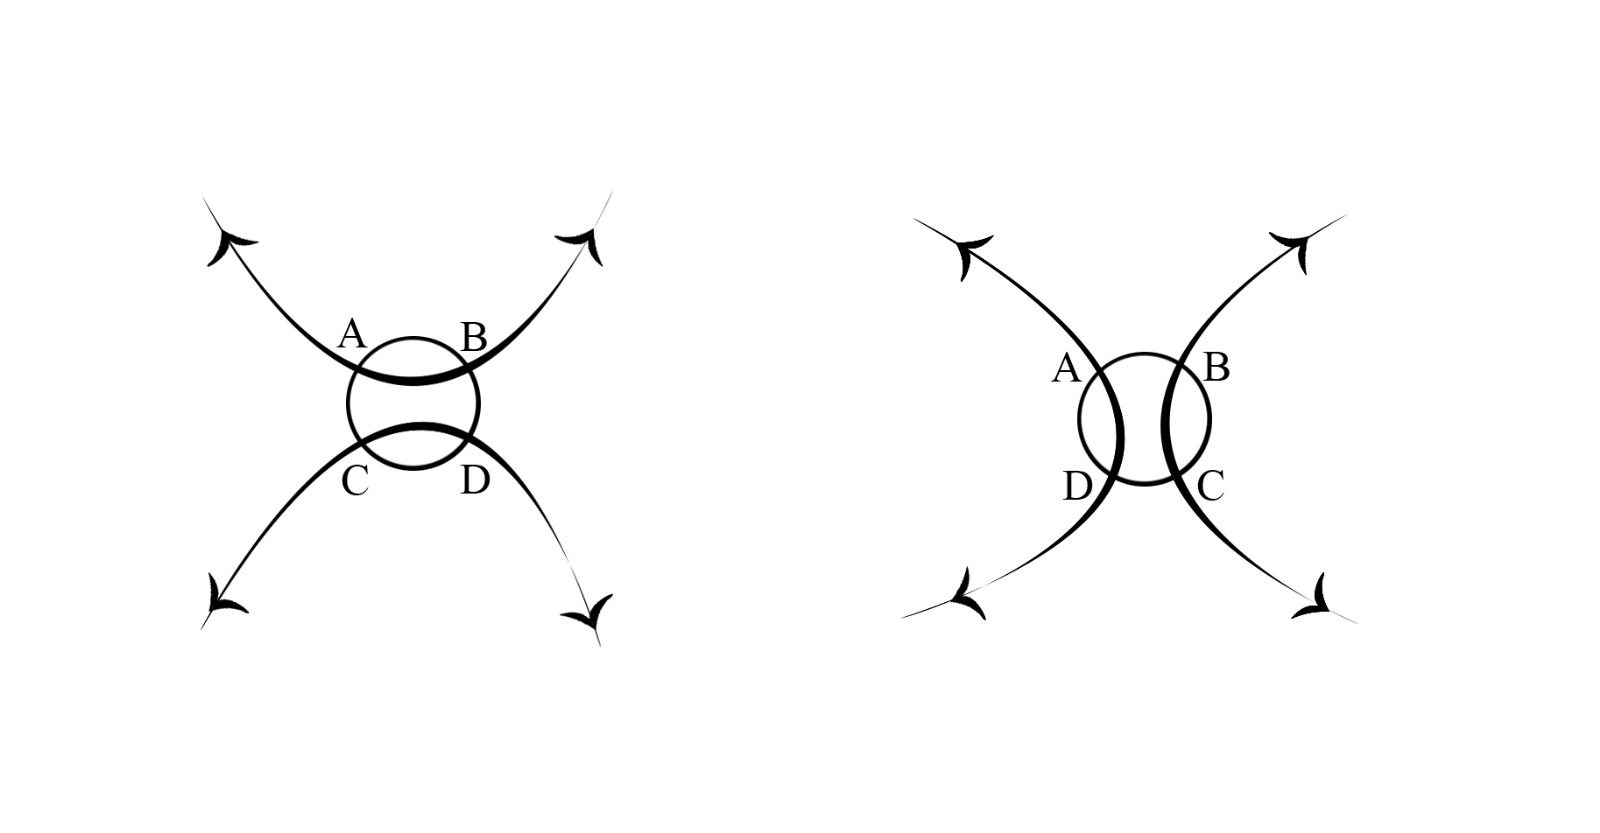
\includegraphics[scale=0.3]{images/2_isotr.jpeg}
    \caption{Basis of $\Inv\bigg(\rho^{\frac{1}{2}}\otimes\rho^{\frac{1}{2}}\otimes\rho^{\frac{1}{2}}\otimes\rho^{\frac{1}{2}}\bigg)=\spann\{v_1,v_2\}$.}
    %\label{fig:enter-label}
\end{figure}

In order to make it computable, in the framework of the multi--linear algebra, we are transposing all the above in the binary basis of $\C^2$, by performing the change of basis 
$$\C^2=\mathop{\spann}_{A=1,2}\{e_A\}=\spann\{\ket{+},\ket{-}\}$$
This way, the support of $\rho$ reads as 
\begin{align*}
{\C^2}^{\otimes 4}
&=\left\{\begin{matrix}
\ket{++++}&&&&&\\
\ket{+++-}&\ket{++-+}&\ket{+-++}&\ket{-+++}&\\
\ket{++--}&\ket{--++}&\ket{+-+-}&\ket{+--+}&\ket{-++-}&\ket{-+-+}\\
\ket{+---}&\ket{-+--}&\ket{--+-}&\ket{---+}&\\
\ket{----}\end{matrix}\right\}\\
&=\mathop{\spann}_{A,B,C,D=1,2}\bigg\{e_A\otimes e_B\otimes e_C\otimes e_D\bigg\}
\end{align*}
and the isotropic subspace $\Inv(\rho)$ results as spanned by
\begin{align*}
    v_1&=\ket{+-+-}-\ket{+--+}-\ket{-++-}+\ket{-+-+}\\
    v_2&=\ket{++--}-\ket{+-+-}-\ket{-+-+}+\ket{--++}
\end{align*}
In this particular basis, a representation of $\SU(2)$ on the support ${\C^{2}}^{\otimes 4}$ can be very easily made explicit through the action of its Lie algebra $\su(2)=\spann\{\tau_1,\tau_2,\tau_3\}$, recalled that $\tau_a:=-\frac{i}{2}\sigma_a$, being $\sigma_a$ the Pauli matrices. Indeed, it holds\footnote{Notice that we are abusing of notation in the following, since we are actually working with a representation $\T\rho^{\nicefrac{1}{2}}:\su(2)\to\GL_2(\C)$ of the Lie algebra of our gauge group, acting on $\C^2=\spann\{\ket{+},\ket{-}\}$ as a matrix $\T\rho^{\nicefrac{1}{2}}(\tau_a)$.}
\begin{equation}\label{tau_i}
    \begin{matrix}
        \tau_1\ket{+}=-\frac{i}{2}\ket{-}&\tau_2\ket{+}=\frac{1}{2}\ket{-}&\tau_3\ket{+}=-\frac{i}{2}\ket{+}\\
        \tau_1\ket{-}=-\frac{i}{2}\ket{+}&\tau_2\ket{-}=-\frac{1}{2}\ket{+}&\tau_3\ket{-}=\frac{i}{2}\ket{-}
    \end{matrix}
\end{equation}
which makes particularly clear how the Lie operators $(L_i)_a:\Kk'\to\Kk'$ act in this framework: they are nothing but the building blocks, defined on a component of the tensor product space, which---via Leibnitz rule---extend the action of the algebra $\su(2)$ on the whole support space $\C^2\otimes\hdots\otimes\C^2$.

Hence, the operator $(L_i)_a$ acts on an element $\ket{\pm\pm\pm\pm}\in{\C^2}^{\otimes 4}$ by transforming the $i$--th component of the state under $\T\rho^{\nicefrac{1}{2}}(\tau_a)$, as ruled in (\ref{tau_i}), i.e.
$$\begin{matrix}
    \T\rho^{{\nicefrac{1}{2}}^{\otimes 4}}:\su(2)\to\End({\C^2}\otimes{\C^2}\otimes{\C^2}\otimes{\C^2})\\
    \tau_a\mapsto (L_i)_a
\end{matrix}$$
where---for $i=0,1,2,3$\footnote{Recall that, by the quantum closure (see Remark \ref{quantum_closure}), it suffices to just compute $i=1,2,3$.}
$$(L_i)_a=\mathbb{1}_2\otimes\hdots\otimes\underbrace{(\tau_a)}_{i\text{--th}}\otimes\hdots\otimes\mathbb{1}_2\in\GL_{2^4}(\C)$$


This allows us to compute the dihedral angle operator $\Dd_{12}=(L_1)_a\delta^{ab}(L_2)_b$ directly restricted to $\Inv(\rho)\subseteq{\C^2}^{\otimes 4}$, as a matrix. By expanding
\begin{align*}
    \Dd_{12}v_k&=(L_1)_1\circ(L_2)_1v_k+(L_1)_2\circ(L_2)_2v_k+(L_1)_3\circ(L_2)_3v_k
\end{align*}
for both $k=1,2$ and by computing Lie operators one by one on them (no matter the order being $\Dd_{ij}$ symmetric), one ends up with the matrix representation of the dihedral operator in the isotropic basis $(v_1,v_2)$, as given by
$${\Dd_{12}}_{|_{\Inv(\rho)}}=\frac{1}{4}\begin{bmatrix}
    3&-2\\
    0&-1
\end{bmatrix}$$

We are now showing that a basis which simultaneously diagonalizes the maximal commuting sub--algebra $(\Dd_{00},\Dd_{11},\Dd_{22},\Dd_{33},\Dd_{12})$ is there, while, e.g., the operator $V^2$ is left non--diagonal. This means, in physical jargon, that the squared areas $\Dd_{\alpha\alpha}$ and the dihedral angle $\Dd_{12}$ show up as compatible observables of the theory, while $V^2$ is not compatible with them, in a pure quantum sense.

For that, it is enough to diagonalize the matrix of $\Dd_{12}$: this yields the two eigenvectors $\bigg(e_{\frac{3}{4}}=v_1, e_{-\frac{1}{4}}=v_1+2v_2\bigg)$, relative to the eigenvalues $\frac{3}{4}, -\frac{1}{4}$ respectively, which clearly gives $\Dd_{12}$ in diagonal form as $\frac{1}{4}\begin{bmatrix}
    3&0\\
    0&-1
\end{bmatrix}$. It can be checked $\bigg(e_{\frac{3}{4}},e_{-\frac{1}{4}}\bigg)$ to be also an eigenbasis for $(L_i)^2=(L_i)_a\delta^{ab}(L_i)_b=-\frac{3}{4}\mathbb{1}:\Gg'\to\Gg'$\footnote{See Remark \ref{Casimir}.}, for each $i=0,1,2,3$, thence they simultaneously diagonalize also the (squared) area operators $\Dd_{00}, \Dd_{11}, \Dd_{22}, \Dd_{33}$. %\newpage
%Consider then each $\C^2=\spann\{\ket{+},\ket{-}\}$, then the isotropic basis element reads in the basis $\ket{\pm}\otimes\ket{\pm}\otimes\ket{\pm}\otimes\ket{\pm}=:\ket{\pm\pm\pm\pm}$ of $W$ as
%\begin{align*}
    %v_1&=\ket{+-+-}-\ket{+--+}-\ket{-++-}-\ket{-+-+}\\
    %v_2&=\ket{++--}-\ket{+-+-}-\ket{-+-+}+\ket{--++}
%\end{align*}
%Thus, being e.g. $\Dd_{13}$ invariant, it results as a finite--dimensional matrix in the isotropic basis, in this case\footnote{We just have to compute $\Dd_{13}={L_{(n,\gamma_1)}}_i\delta^{ij}{L_{(n,\gamma_3)}}_j$ and explicit the action of $\tau_i$ on the basis of $W$, from which it results $\Dd_{13}(v_1)=-\frac{1}{4}(v_1+2v_2)$, $\Dd_{13}(v_2)=-\frac{1}{4}(2v_1+v_2)$.}
%$$\Dd_{13}=\frac{1}{4}\begin{bmatrix}
   %-1&-2\\
   %-2&-1
%\end{bmatrix}$$
%which diagonalizes as $\Dd_{13}=\begin{bmatrix}
    %-\frac{3}{4}&0\\
    %0&\frac{1}{4}
%\end{bmatrix}$ with respect to the eigenbasis $e_{-3}=v_1+v_2$ and $e_1=v_1-v_2$. 

%Moreover, the whole isotropic subspace $\spann\{v_1,v_2\}$ results to be an eigenspace of the area operator operator of each link, being $\Dd_{\alpha\alpha}={E_\alpha}^2=\frac{3}{4}(\hslash\boldsymbol{\kappa\gamma})^2\mathbb{1}$ on invariant states. Now, the closure condition implies $L_1\cdot L_2\times L_0=-L_1\cdot L_2\times L_3$ and we can also compute, for the dihedral angle $\Dd_{12}$ 
%$$L_1\cdot L_2\,v_1=-\frac{3}{4}v_1\qquad L_1\cdot L_2\,v_2=\frac{1}{4}(v_2-2v_1)$$ 
%and then find the eigenbasis $(e_1,e_2)=(v_1,v_1-2v_2)$ which diagonalizes  $\Dd_{12}$ as
%$$\Dd_{12}=\begin{bmatrix}
    %-3&0\\
    %0&1
%\end{bmatrix}$$
%as well as the areas. %$\Dd_{\alpha\alpha}e_1=\frac{3}{4}(\hslash\boldsymbol{\kappa\gamma})^2e_1$ and $\Dd_{\alpha\alpha}e_2=\frac{3}{4}(\hslash\boldsymbol{\kappa\gamma})^2e_1$ diagonalized also the areas. 
On the other hand, the matrix representing $\Dd_{13}$, which does not commute with $\Dd_{12}$ as operator, writes in the basis $\bigg(e_{\frac{3}{4}},e_{-\frac{1}{4}}\bigg)$ as %$\frac{1}{4}\begin{bmatrix}
   %-2&3\\
  % 1&0
%\end{bmatrix}$ (questo era il mio calcolo ma meglio non fidarsi)
$\frac{1}{4}\begin{bmatrix}
    0&3\\1&2
\end{bmatrix}$, which in fact is not diagonal. In the end, we can compute the volume squared given in (\ref{volume_op}) in such a basis, which results as the non--diagonal matrix---being $\bigg[\Dd_{13},\Dd_{12}\bigg]=\frac{1}{8}\begin{bmatrix}
   0&-1\\
   -3&0
\end{bmatrix}$ in the basis $\bigg(e_{\frac{3}{4}},e_{-\frac{1}{4}}\bigg)$ %\footnote{We recommend \cite{LN9} for the complete computations.}
%$$V^2=\frac{2i\hslash}{9}\begin{bmatrix}
 %   0&0\\
 %   1&0
%\end{bmatrix}$$ (sempre i miei ma meglio non fidarsi)
$$V^2=\frac{i\hslash}{36}\begin{bmatrix}
    0&1\\
    3&0
\end{bmatrix}$$
Accordingly, it is left fuzzy.
%Accordingly, we have provide an eigenbasis of isotropic vectors for the product representation $\rho^{\nicefrac{1}{2}}\otimes\rho^{\nicefrac{1}{2}}\otimes\rho^{\nicefrac{1}{2}}\otimes\rho^{\nicefrac{1}{2}}$, which simultaneously diagonalize the four squared areas $\Dd_{00}$, $\Dd_{11}$, $\Dd_{22}$, $\Dd_{33}$ and the dihedral angle $\Dd_{12}$, though the squared volume $V^2$ is left fuzzy.

\begin{remark}[Discreteness of volume operator]
    We have just realized how the area operators come with a discrete spectrum---see \emph{(\ref{area_spec})}. The same argument applies also to $V^2$; indeed, its eigenvalues are real and positive, hence it is a positive definite self--adjoint operator defined on $\Gg'$. This way, the \emph{volume operator} is well--defined as $V:=\sqrt{V^2}$, which accounts for a discrete spectrum.
\end{remark}

As a matter of fact, there are shreds of evidence that for any choice of an invariant maximal sub--algebra of compatible operators, we can find a basis of invariant states in $\Gg'$ which diagonalize simultaneously $5$ observables, leaving the sixth uncertain. 



\newpage
\section{Explorations into the quantum geometry of space}
In this final section, we delve into the geometry of space at the Planck scale. We will build upon the deductions inferred about the geometry of space, starting from the uncertainty principle within this context. This exploration tries to examine something that can approximate the idea of a classical limit in the framework of \emph{quantum tetrahedra}---being finally defined as open spin networks with one node of valence $4$---providing an attempt to shed light on the transition from quantum to classical geometrical descriptions of space.

%\subsection{Overviewing the next steps}
As mentioned, the uncertainty principle recovered in the discussion on Section 3.2.2 about the quantum geometry of tetrahedra highlights the presence of a $1$--parameter family of tetrahedra's geometries for---e.g.---areas and volume fixed, describing some orbit in the homogeneous space $\Geo$, parametrized by the uncertain dihedral angle.

This can be indeed proved\footnote{Let us fix gauge covariance so that
$$\begin{cases}
    \l_1=\lambda\mathbf{i}\\
    \l_2=\lambda(\alpha\mathbf{i}+\beta\mathbf{j})\\
    \l_3=\lambda(\gamma\mathbf{i}+\delta\mathbf{j}+\epsilon\mathbf{k})&\lambda,\beta>0
\end{cases}$$
Being $\Geo=\nicefrac{\GL^+(3)}{\SO(3)}$, hence the basis $(\l_1,\l_2,\l_3)$ must be positive, then it is $\alpha,\gamma,\delta>0$ which also implies $\epsilon>0$. We know that vectors $\l_i$ are completely determined (up to gauge transformations in $\SO(3)$) by the dihedral angles since each one of the six parameters $\lambda,\alpha,\hdots,\epsilon$ depend on $\d_{ij}$s.

By recalling the isomorphism $T_{[x]}\Geo\cong\R^6$ and fixing the areas $\d_{\alpha\alpha}$ and the volume $\d$ as a maximal commuting sub--algebra of ---e.g.---$\bigg\{\d_{\alpha\alpha},\d,\d_{12}\bigg\}_{\alpha=0,1,2,3}$, this gauge yields
$$\begin{cases}
    \d_{00}=\lambda^2\bigg(1+\alpha^2+\beta^2+\gamma^2+\delta^2+\epsilon^2+2\alpha+2\gamma+2\alpha\gamma+2\beta\delta\bigg)\\
    \d_{11}=\lambda^2\\
    \d_{22}=\lambda^2(\alpha^2+\beta^2)\\
    \d_{33}=\lambda^2(\gamma^2+\delta^2+\epsilon^2)\\
    \d=\det(\Delta) \\
\end{cases}$$
where $\Delta:=(\d_{ij})_{i,j=1,2,3}$, from which follows
$$\begin{cases}
    \d_{12}=\lambda^2\alpha\\
    \d_{13}=\lambda^2\gamma=\frac{\gamma}{\alpha}\d_{12}\\
    \d_{23}=\lambda^2(\alpha\gamma+\beta\delta)=\d_{12}\gamma+\lambda^2\beta\delta
\end{cases}$$
}, resulting in

\begin{equation}
    \begin{cases}
    \d_{11}=\frac{\d_{12}^2}{\alpha^2}\\
    \d_{22}=\d_{12}^2+\lambda^2\beta^2\\
    \d_{33}=\d_{12}^2\frac{\gamma^2}{\alpha^2}+\lambda^2\delta^2+\lambda^2\epsilon^2\\
    \d_{00}=\bigg(1+\frac{1}{\alpha^2}+\frac{\gamma^2}{\alpha^2}\bigg)\d_{12}^2+\bigg(2+\gamma+\frac{\gamma}{\alpha}\bigg)\d_{12}+\lambda^2\bigg(\beta^2+\delta^2+\epsilon^2+\beta\delta\bigg)\\
    \d=\d_{12}\frac{\gamma}{\alpha}\epsilon\\
    \d_{12}=\d_{12}
\end{cases}
\end{equation}
These are parametric equations in $\Geo$ that induce a cartesian--like system of equations $\Phi(\d_{\alpha\alpha},\d,\d_{12})=0$, describing a $6-5=1$--dimensional subspace, for a given functional $\Phi$ of $\Geo$, in the same flavour of Theorem \ref{T^*Geo}. 

Hence, by fixing $\d_{12}=:\theta\in\R$ as a parameter, equations $(3.13)$ are just parametrizing a curve $\theta\mapsto\phi(\d_{\alpha\alpha},\d,\theta)$ in the configuration space of the theory\footnote{Recall that, for a given configuration space $Q$, physical observables are functions of the phase space $T^*Q$. In our case, $Q=\Geo$ where $\d_{ij}$ are there as lagrangian coordinates.

Notice also that we can actually regard $\d_{\cdot\cdot}\in T^*\Geo$ as bilinear map on $\Geo$.}, which corresponds to a $1$--parameter family of tetrahedra moving on a $\S^1$--orbit.%\footnote{Ci vuole una giustificazione}.

\subsection{Quantum states of spin $(j_1,j_2,j_3,j_4)$ tetrahedra}

Here, one can resume the quantum interpretation, exploring what happens to the angle $\theta$ as the spins increase---whether it spreads or shrinks, e.g. This investigation is %somewhat akin
almost like studying the classical limit of our theory, as we expect that the tetrahedron with spins $(\frac{1}{2},\frac{1}{2},\frac{1}{2},\frac{1}{2})$ represents the smallest possible chunk of space at the Planck scale. As the spins grow, we should eventually recover the geometry of a classical tetrahedron.

The following result shows how the spin $(j,j,j,j)$ tetrahedron writes as a superposition of $2j+1$ spin networks.

\begin{teo}\label{eddy}
Let $\rho=\bigotimes_{i=1}^4(\rho^j)_i$ be the product $4$--times of the spin--$j$ irreducible representation of $\SU(2)$ and let $\Inv(\rho)$ be the subspace of the support of $\rho$ made of isotropic vectors. Then
    $$\dim(\Inv(\rho))=2j+1$$
\end{teo}
\begin{proof}%[Sketch of proof]
The representation $\rho$ writes through the symmetric representation as $$\bigotimes_{i=1}^4\Sym^{2j}=\bigotimes_{i=1}^4\bigg(\bigodot_{k=1}^{2j}{\rho^{\frac{1}{2}}}\bigg)$$
having dimension $(2j+1)^4$. Recall that Theorem \ref{intert_isotrop} has showed up a one--to--one correspondence between intertwiners of fundamentals $\rho^{\frac{1}{2}}$ appearing in the product and isotropic generators of $\Inv(\rho)\subseteq\C^{(2j+1)^4}$.\, Applying Clebsch--Gordan theorem \ref{glebsh} to our $\rho$ yields

$$\rho=\bigoplus_{i=0}^{2j}\rho^{2j-i}\otimes\bigoplus_{i'=0}^{2j}\rho^{2j-i'}%=\bigoplus_{i,i'=0}^{2j}\rho^{2j-i+2j-i'}
$$
and conditions for the non--triviality of $\Inv(\rho)$ turn out to be equivalent to the Diophantienne equation $2j-i=2j-i'$, whose solutions are parametrized by a semi--integer $l=0,\frac{1}{2},1,\hdots,j$ satisfying $i=i'=2l\in\N$. 

The thesis is now easily proved by proceeding by induction on the spin $j\in\frac{1}{2}\N$, regarding the statement on the dimension of $\Inv(\rho)$ in a Clebsch--Gordan fashion, by noticing that as the label $l$ increases by half integers steps, being bounded from above by $j$, the number of possible steps allowed for $l$ are exactly $2j+1$ and correspond to how many linear independent $\rho$--isotropic vectors are there, i.e. $$\Inv(\rho)=\spann_l\{v_l\}$$
\begin{itemize}
    \item The first non--trivial case holds for $j=\frac{1}{2}$ which indeed allows a $2$--dimensional isotropic subspace, the basis vectors being parametrized by $l=0\,\leftrightarrow\,i=i'=0$ and $l=\frac{1}{2}\,\leftrightarrow\,i=i'=1$, hence, the base case is satisfied.
    
    For instance, to $j=1$ corresponds the sequence 
    $$\begin{matrix}
        l=0&\Rightarrow&i=i'=0\\
        l=\frac{1}{2}&\Rightarrow&i=i'=1\\
        l=1&\Rightarrow&i=i'=2
    \end{matrix}$$
$$\vdots$$
\item For a generic spin $j\in\frac{1}{2}\N$ we get
$$\begin{matrix}
        l=0&\Rightarrow& i=i'=0\\
        l=\frac{1}{2}&\Rightarrow&i=i'=1\\
        l=1&\Rightarrow&i=i'=2\\
        l=\frac{3}{2}&\Rightarrow&i=i'=3\\
        \vdots&\,&\vdots\\
        l=j&\Rightarrow&i=i'=2j
    \end{matrix}$$
\end{itemize}
and Theorem \ref{intert_isotrop} concludes the proof.

Notice that, in the graphic representation, the coupled indices $i,i'$  are in place to labelling the number of possible exchanges among the threads which belong to the upper part of the node with the ones in the lower part and each coupling corresponds to a linear independent spin network.
%Let us now assume by inductive hypothesis that $\Inv\bigg({\rho^{j-1}}^{\otimes4}\bigg)=\spann\{v_1,\hdots,v_{2j-1}\}$, for a generic semi--integer $j$. Thence, the above Clebsch--Gordan argument yields
%$${\rho^{j-1}}^{\otimes4}=\bigoplus_{i=0}^{2j-2}\rho^{2j-2-i}\otimes\bigoplus_{i'=0}^{2j-2}\rho^{2j-2-i'}$$
%from which the inductive hypothesis results as equivalent to the Diophantienne equation $2j-2-i'=2j-2-i\,\Leftrightarrow\, i=i'\in\N$, i.e. solutions are parametrized by $2l\in\N$, for some half integer $l=0,\frac{1}{2},1,\hdots,2j$ such that $\spann_{l}\{v_l\}=\Inv\bigg({\rho^{j-1}}^{\otimes4}\bigg)$. 
%This way, reiterating the above argument on $\rho$ gives a set of Diophantienne equations on the form $2j-i=2j-i'$ being solved by all the previous--case--solutions labelled by $l\in\frac{1}{2}\N\,:\,l\leq2j$, plus the solution $i=i'=4j+2\leftrightarrow l=2j+1$, which does not solve $2j-2-i'=2j-2-i$. Overall, such solutions are labelled by an integer $2k\in\N$, for some $k=0,\frac{1}{2},1,\hdots,2j+2$, and Theorem \ref{intert_isotrop} concludes $\Inv(\rho)=\spann_k\{v_k\}$.
\end{proof}
\newpage
\subsubsection{Quantum tetrahedron $(\frac{1}{2}, \frac{1}{2}, \frac{1}{2}, \frac{1}{2})$: the ground state}

As a matter of fact $\rho={\rho^{\frac{1}{2}}}^{\otimes4}$ is the smallest possible invariant state the theory allows, corresponding to quantum tetrahedra on the form $(\frac{1}{2}, \frac{1}{2}, \frac{1}{2}, \frac{1}{2})$ resulting as a superposition of two spin networks, as follow---CFR. Figure 3.4

\begin{figure}[ht]
    \centering
    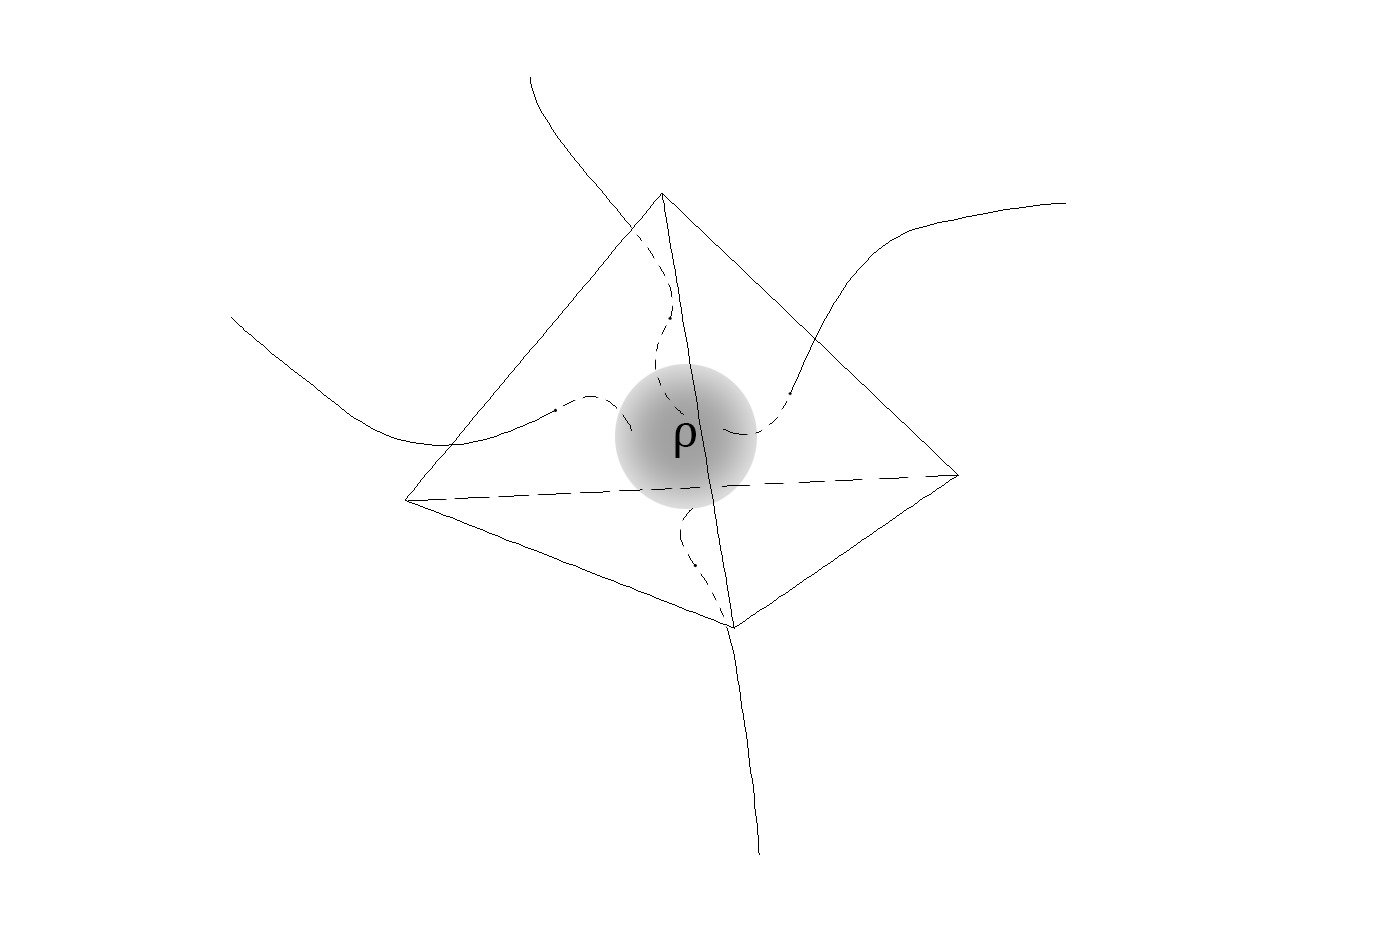
\includegraphics[scale=0.3]{images/1half_tetrahedron.jpeg}
    %\caption{The quantum tetrahedron $(\frac{1}{2},\frac{1}{2},\frac{1}{2},\frac{1}{2})$ as the superposition of spin networks spanning $\Inv\bigg(\rho^{\frac{1}{2}}^{\otimes4}\bigg)$ in Figure 3.4.}
\end{figure}

We already discussed this case widely in the previous section. Theorem \ref{eddy} bears out that $\dim(\Inv(\rho))=2$, being in fact spanned by the corresponding two linear independent $\rho$--isotropic vectors of ${\C^2}^{\otimes4}$, that we now express, for later convenience, as follow
\begin{align*}
    v_1&=\sum_{A,B,C,D=1,2}\ket{\wick{\c1{A}\,\c1{B}\,\c2{C}\,\c2{D}}}\\
    v_2&=\sum_{A,B,C,D=1,2}\ket{\wick{\c1{A}\,\c2{B}\,\c2{C}\,\c1{D}}}
\end{align*}
Being our geometric algebra of observables made of operators that represent as symmetric finite--dimensional squared matrices, once they are restricted on the support of the representation $\rho$, it is appropriate to compute them with respect to an orthonormal basis\footnote{In fact, the subspace $\Inv(\rho)$ is not orthonormal, being 
$$\langle v_1|v_2\rangle=2\quad\text{and}\quad \langle v_1|v_1\rangle=4=\langle v_2|v_2\rangle$$
where we are just using the canonical inner product induced by the linear isomorphism among ${\C^2}^{\otimes4}$ and $ \C^{16}$---see Appendix A for details.}. 

The Gram--Schmidt algorithm, for instance, provides us with invariant operators $\Dd_{12}, \Dd_{13}$ in the resulting orthonormal basis of spin networks $(E1,E2)$ as represented by the matrices
$$\Dd_{12}=\frac{1}{4}\begin{bmatrix}
        3&0\\
        0&-1
\end{bmatrix}\qquad\text{and}\qquad\Dd_{13}=\frac{1}{4}\begin{bmatrix}
    0&\sqrt{3}\\
    \sqrt{3}&2
\end{bmatrix}$$
yielding the volume squared operator, up to a real constant and sign, on the form
$$i\bigg[\Dd_{13},\Dd_{12}\bigg]=\frac{i}{4}\begin{bmatrix}
    0&-\sqrt{3}\\
    \sqrt{3}&0
\end{bmatrix}$$
which diagonalizes as $V^2=\frac{2i\hslash}{9}\frac{\sqrt{3}}{4}\Biggl|\begin{bmatrix}
    -1&0\\
    0&1
\end{bmatrix}\Biggl|$ with respect to the eigenvectors basis $(e_{-1}, e_{+1})$, where
$$e_{-1}=E_2-E_1\quad\text{and}\quad e_{+1}=E_1+E_2$$

This basis also fixes all the (normalized) squared areas to $\Dd_{\alpha\alpha}e_{-1}=-\frac{3}{4}e_{-1}$ and $\Dd_{\alpha\alpha}e_{+1}=-\frac{3}{4}e_{+1}$ as being compatible with the squared volume, each face having area $\frac{\sqrt{3}}{2}$---CFR. (3.6). The free dihedral angle, instead, should be left fuzzy as an operator and in fact it results non diagonal with respect to the basis $(e_{-1},e_{+1})$, as $\Dd_{12}=\frac{1}{2}\begin{bmatrix}
    1&-2\\
    -2&1
\end{bmatrix}$\footnote{All the previous and following computations are Python--verified---see on Github \href{Joyboy0056/QuantumGeometryofTetrahedra}{https://github.com/Joyboy0056/QuantumGeometryofTetrahedra}.}.  

At this stage one is able to compute the mean values and the variance of $\Dd_{12}$ in the ground state representation---see forthcoming \cite{LNX}.

\subsubsection{Excited states of quantum tetrahedra}
The same argument applies to the cases of higher spins quantum tetrahedra 

$$\bigg(1,\frac{1}{2},\frac{1}{2},1\bigg),\,\bigg(1,1,1,1\bigg), \,\bigg(\frac{3}{2},1,1,\frac{3}{2}\bigg),\,\bigg(\frac{3}{2}, \frac{3}{2}, \frac{3}{2}, \frac{3}{2}\bigg), \,\hdots$$
Computations here get very hard quickly, since Theorem \ref{eddy} glimpses the dimensions of the matrices representing our geometric operators to increase exponentially.
For instance, the spin $(j,j,j,j)$ quantum tetrahedra ${\rho^1}^{\otimes4}$ and ${\rho^{\frac{3}{2}}}^{\otimes4}$ are supported in complex vector spaces of dimension $81$ and $256$, respectively, and certainly bring along a huge mole of new vectors to take into account, compared with the $16$--dimensional case offered by the ground state tetrahedron ${\rho^{\frac{1}{2}}}^{\otimes4}$.\\

However, the simplest excited state $\rho=\rho^1\otimes\rho^{\frac{1}{2}}\otimes\rho^{\frac{1}{2}}\otimes\rho^1$ is supported on a $3^2\cdot2^2=36$--dimensional complex vector space and its isotropic subspace $\Inv(\rho)$ can be seen to be still $2$--dimensional, thence all the geometric invariant operators still appear as manageable $2\times2$ matrices and one could compute mean values and variance as in the previous understood case.\\

The very first different case, from the viewpoint of the dimensions, results in the spin $(1,1,1,1)$ tetrahedron, pictured in Figure 3.5, whose geometric observables turn out to be represented by $3\times3$ matrices, as Theorem \ref{eddy} assures.
\begin{figure}[ht]
    \centering
    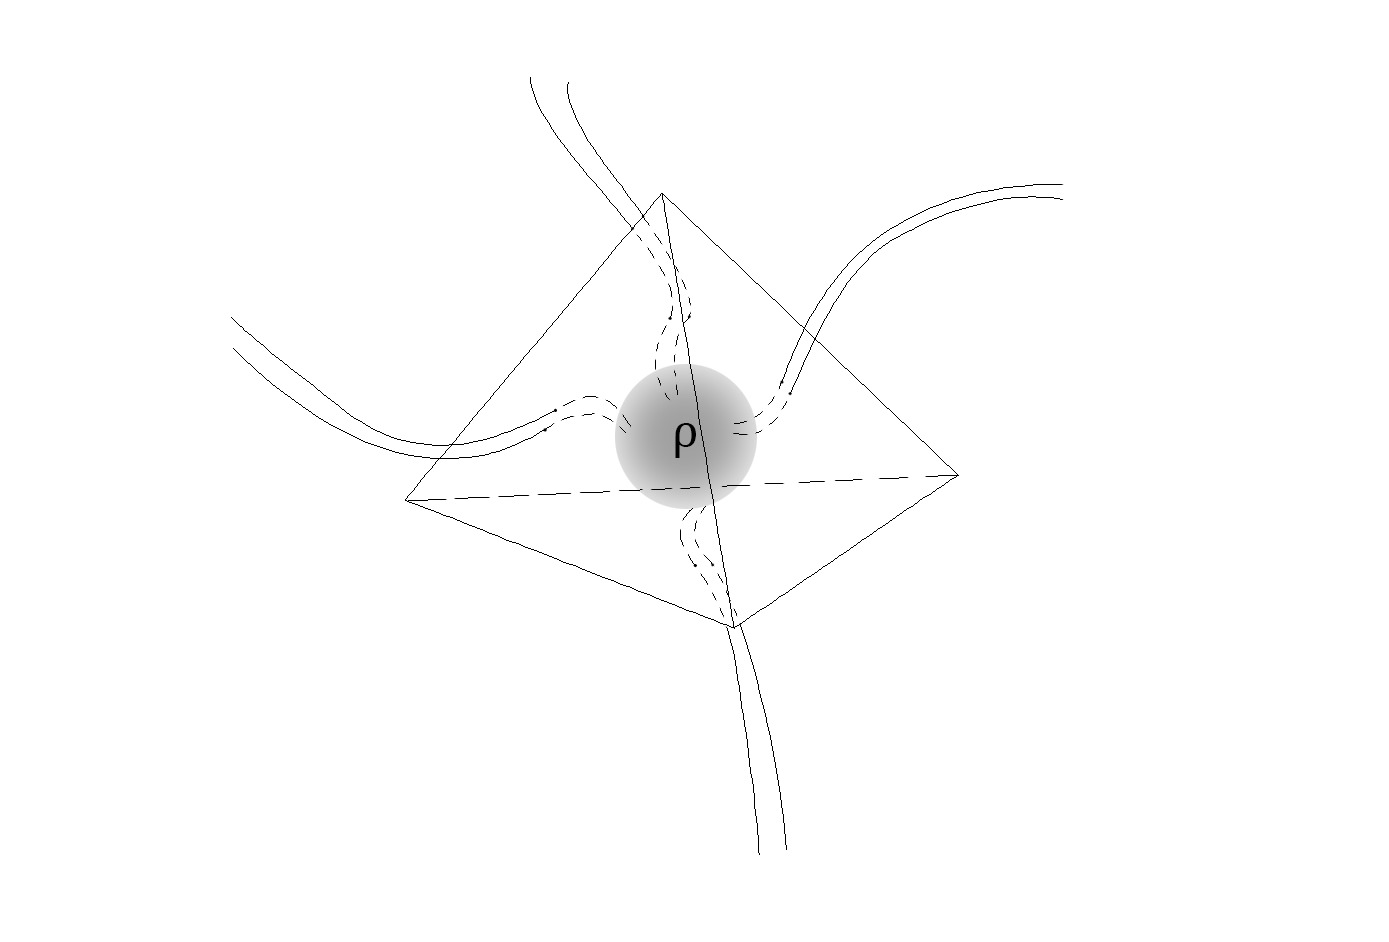
\includegraphics[scale=0.3]{images/1_tetrahedron.jpeg}
    \caption{The quantum tetrahedron $(1,1,1,1)$.}
\end{figure}
\,\newline
The treatment of this spin $(1,1,1,1)$ case requires to represent Lie operators, the building blocks of geometric algebras, in the correct support space. For that, one observes that $\C^2\otimes\C^2=\spann_{A,B=1,2}\{\ket{A\,B}\}$ allows an invariant subspace on the form 
\begin{equation}\label{C3_subspace}
\begin{split}
    \C^2\odot\C^2&=\spann\Biggl\{\ket{++},\tiny{\frac{\sqrt{2}}{2}}\Biggl(\ket{+-}+\ket{-+}\Biggl),\ket{--}\Biggl\}\\
    &\cong\spann\{\ket{1},\ket{0},\ket{-1}\}\cong\C^3
\end{split}    
\end{equation}\label{C3_subspace}
supporting adjoint representations $\rho^1=\Sym^2:\SU(2)\to\End(\C^3)$. 

This way, we can directly write down expressions for the Lie operators in this bigger representation, still by using $(\ref{tau_i})$  extended along the above isomorphism through
$$L^a\ket{i}=L^a\ket{AB}=L^a\ket{A}\otimes\ket{B}+\ket{A}\otimes L^a\ket{B}$$
from which we get $\T\rho^1(\su(2))$ as the subspace of $\GL_3(\C)$ being spanned by matrices represented in the basis $\{\ket{i}\}_{i=1,0,-1}$ as
$$L^1=-\frac{i\sqrt{2}}{2}\begin{bmatrix}
    0&1&0\\
    1&0&1\\
    0&1&0
\end{bmatrix}\qquad L^2=\frac{\sqrt{2}}{2}\begin{bmatrix}
    0&-1&0\\
    1&0&-1\\
    0&1&0
\end{bmatrix}\qquad L^3=\begin{bmatrix}
    -i&0&0\\
    0&0&0\\
    0&0&i
\end{bmatrix}$$
The quantum tetrahedron corresponding to $\rho=\bigotimes_{i=1}^4(\rho^1)_i=\bigotimes_{i=1}^4(\rho^{\frac{1}{2}}\bigodot\rho^{\frac{1}{2}})_i$ can be easily seen to allow, by Theorem \ref{intert_isotrop}, the three independent spin networks to span $\Inv(\rho)$, as in the following Figure 3.6
\begin{figure}[ht]
    \centering
    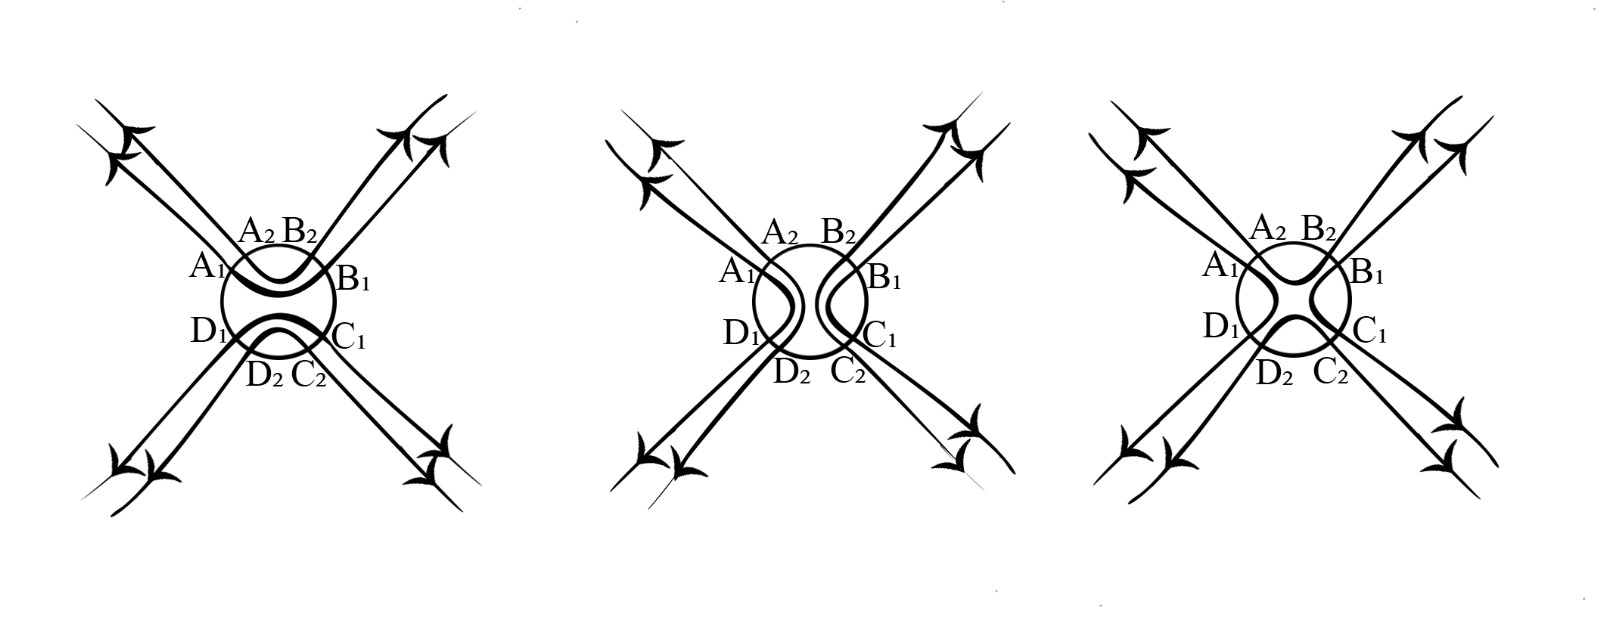
\includegraphics[scale=0.3]{images/3_isotr.jpeg}
    \caption{Basis of $\Inv\bigg(\rho^1\otimes\rho^1\otimes\rho^1\otimes\rho^1\bigg)=\spann\{v_1,v_2,v_3\}$.}
    %\label{fig:enter-label}
\end{figure}
\,\newline
which explicitly write as
\begin{align*}
    v_1&=\epsilon^{A_1B_1}\epsilon^{A_2B_2}\epsilon^{C_1D_1}\epsilon^{C_2D_2}\ket{A_1\,A_2|B_1\,B_2|C_1\,C_2|D_1\,D_2}\\
    &=\sum_{A_i,B_i,C_i,D_i=1,2}\ket{\wick{\c1{A_1}\,\c2{A_2}|\c1{B_1}\,\c2{B_2}|\c1{C_1}\,\c2{C_2}|\c1{D_1}\,\c2{D_2}}}
\end{align*}
\begin{align*}
    v_2&=\epsilon^{A_1D_1}\epsilon^{A_2D_2}\epsilon^{B_1C_1}\epsilon^{B_2C_2}\ket{A_1\,A_2|B_1\,B_2|C_1\,C_2|D_1\,D_2}\\
    &=\sum_{A_i,B_i,C_i,D_i=1,2}\ket{\wick{\c1{A_1}\,\c2{A_2}|\c3{B_1}\,\c4{B_2}|\c3{C_1}\,\c4{C_2}|\c1{D_1}\,\c2{D_2}}}    
\end{align*}
\begin{align*}
    v_3&=\epsilon^{A_1D_1}\epsilon^{A_2B_2}\epsilon^{B_1C_1}\epsilon^{C_2D_2}\ket{A_1\,A_2|B_1\,B_2|C_1\,C_2|D_1\,D_2}\\
    &=\sum_{A_i,B_i,C_i,D_i=1,2}\ket{\wick{\c1{A_1}\,\c2{A_2}|\c4{B_1}\,\c2{B_2}|\c4{C_1}\,\c3{C_2}|\c1{D_1}\,\c3{D_2}}}\\
\end{align*}
%$$\vdots$$
%$$\Inv\bigg({\rho^{\nicefrac{1}{2}}}^{\otimes 4}\bigg)=\spann\{v_1,v_2\}$$
%$$\Dd_{12}\Biggl|_{\Inv\bigg(\rho^{{\nicefrac{1}{2}}^{\otimes 4}}\bigg)}=\frac{1}{4}\begin{bmatrix}
    %3&-2\\
    %0&-1
%\end{bmatrix}$$
%$$\Dd_{13}\Biggl|_{\Inv\bigg(\rho^{{\nicefrac{1}{2}}^{\otimes 4}}\bigg)}=\frac{1}{4}\begin{bmatrix}
    %1&2\\
    %2&1
%\end{bmatrix}$$
%$$\Rightarrow\quad\bigg[\Dd_{13},\Dd_{12}\bigg]\Biggl|_{\Inv\bigg(\rho^{{\nicefrac{1}{2}}^{\otimes 4}}\bigg)}=\frac{1}{4}\begin{bmatrix}
    %1&-2\\
    %2&-1
%\end{bmatrix}$$
%$$\Rightarrow\quad V^2\Biggl|_{\Inv\bigg(\rho^{{\nicefrac{1}{2}}^{\otimes 4}}\bigg)}=\frac{i\hslash}{18}\begin{bmatrix}
   % 1&2\\
   % 2&1
%\end{bmatrix}$$
%An eigenbasis of $V^2$ restricted to the quantum tetrahedra isotropic subspace is so given by $(e_1=v_1+v_2, e_2=v_2-v_1)$ with eigenvalues  $\frac{i\hslash}{18}(3,-1)$ respectively. 
%Negative measurements for the volume squared? How to define the volume? Remark 3.2.1 falls?
%What's next: mettiti nella base $(e_1,e_2)$ che diagonalizza il volume come $V^2\Biggl|_{(e_1,e_2)}=\frac{i\hslash}{18}\begin{bmatrix}
   % 3&0\\
    %0&-1
%\end{bmatrix}$ e contemporaneamente anche le aree $\Dd_{\alpha\alpha}$ (dimostra il conto con Python) e calcola su questa base un operatore di diedro che non commuta, mostrando che non è in forma diagonale.
%$$\vdots$$
%Prova ad aumentare gli spin e a rifare i conti sugli operatori: occhio che forse su $\rho={\rho^1}^{\otimes 4}$ si ha $\dim\Inv(\rho)=3$, quindi le matrici sono $3\times3$.
%Adesso, si può pensare di aumentare gli spin del tetraedro e vedere come la media e la varianza dell'angolo diedro lasciato incerto variano al crescere degli spin: puoi fare un commento su cosa ci si aspetta.
%Condisci il discorso con dei risultati interessanti sul caso del tetraedro $\rho={\rho^j}^{\otimes4}$ e mostra il risultato $\dim(\Inv(\rho))=2j+1$ e che gli operatori invarianti qui saranno matrici $2j+1\times2j+1$.
We can now find the correspondent expression of $v_1,v_2,v_3$ in the basis $$\{\ket{i|j|k|l}\}_{i,j,k,l=1,0,-1}$$
on which we can make fundamental Lie operators $L^a$ act component--wise as
$$(L_i)^a=\1_3\otimes\hdots\otimes \underbrace{L^a}_{i-\text{th}}\otimes\hdots\otimes\1_3\in\GL_{81}(\C)$$
and eventually reconstruct our invariant geometric algebra made of polynomials in the dihedral angles  $\Dd_{ij}=(L_i)^a\delta_{ab}(L_j)^b$, resulting here as $3\times3$ symmetric matrices. Thence, one can apply the above argument discussed in the case of the ground state tetrahedron, so on and so forth, for any possible tetrahedron of spin $(j_1,j_2,j_3,j_4)$ allowing a suitable invariant subspace of isotropic vectors.\\

In the end, LQG claims to be a generally covariant QFT whose quantum observables are geometric quantities, here yet in space. This brings hope that, by repeating the argument for the whole spacetime, we will achieve a complete quantum description of the gravitational field, which \emph{is} the geometry of spacetime, according to GR. 

On top of that, lengths, areas and volumes appear as discretized quantities with precise values to be assumed in operators' spectra and only within a quantum state of the gravitational field. At this stage, the one--to--one correspondence among classical geometries of tetrahedra and quantum geometries---appearing here as a framework where operators on gauge (and diffeo) invariant states can be described---carries spin networks of valence $4$ (aka, quantum tetrahedra) comes very clear and the whole machinery is set within the scenario of multilinear algebra, where everything is computable.




\chapter*{Conclusions and Perspectives}
\markboth{\MakeUppercase{Conclusions and Perspectives}}{}
\addcontentsline{toc}{chapter}{Conclusions and Perspectives}
The first conclusion of LQG is that GR and QM do not contradict each other. A quantum theory that reduces to GR as its classical limit seems to exist. The work was not small and more is needed to represent the dynamics, but, in the end, a theory was produced which, more than merging GR and QM, it coherently adapts the generally relativistic aspects of GR to a quantization process, which is in general mathematically ill--posed.\, What is fundamental is that LQG follows in many aspects the deductive process that led Einstein himself to his revolutionary geometric theory of gravity, and chooses to best preserve its covariance characteristics and adapt them to a quantum interpretation. Of course, this could not be done by avoiding the choice of some physical postulates---which in this case has been to represent quantum states discretized on lattices---whose truthfulness actually shapes the theory, which can only be proven true by experiments (CFR. \cite{baggot}).\, While LQG may not offer the definitive quantum portrait of spacetime, it undeniably stands as a well--founded proposal for a generally covariant quantum field theory, particularly from a mathematical perspective. The dynamical nature of the spacetime metric field mandates its determination through field equations, eschewing a--priori fixation and safeguarding the foundational tenet of background--independence throughout the quantisation process. %Although it does not turn out to be the true quantum description of spacetime, LQG is certainly a first and working proposal for a generally covariant quantum field theory, at least from a mathematical point of view. Indeed, the spacetime metric field, being a dynamical variable, must be determined a--posteriori by field equations, and cannot be a--priori fixed. 

Technically speaking, we had a gauge--natural field theory in $\mathcal{F}(P)\times_{\M^{1,3}}\Con(P)$, with structure bundle $P\to\M^{1,3}$ being a principal $\SL(2,\C)$--bundle over the spacetime, in the dynamical variables $(e^I,\omega^{IJ})$, so--called Holst theory, being constrained by both the gauge and the diffeomorphism covariance. As a matter of fact, Holst theory, being dynamically equivalent to GR, also imposes topological obstructions on the spacetime, which has to be globally hyperbolic, hence a farther constraint appears, related to the evolution in time of space. Once the constraint equations have been grossed up, such a theory reduces to a $\SU(2)$--gauge--natural theory in the dynamical variables $(e^a,\kappa^i,\A^i)$, the physical states being represented by gauge equivalence classes of $\SU(2)$--connections $[\A]$ on the leaves of a foliation of $\M^{1,3}$, which turn out to be space--like by construction, with respect to the metric induced by the frame $e^a$. At this stage, the quantization procedure is initiated by discretizing the gauge field $\A$, paving the way for the construction of the Hilbert quantum space. Here, kinematical states are defined as $\SU(2)$--functionals $\Psi[\A]$, embodying the foundational principles of quantum mechanics. Imposing the symmetries encoded in the constraint equations, we ensure compliance with the main axioms of quantum mechanics within the confines of a separable Hilbert space of gauge and $\Diffeo_*$ covariant states representing the gravitational field.\, In the end, operators that restrict to the invariant states turn out to correspond to a Lie algebra of geometric observables which stand for the quantisation of the classical geometry of a tetrahedron. The overarching perspective offered by LQG is that the gravitational field, at its core, is depicted through quantum spin networks intricately woven on lattices of $4$--valence nodes, the links being represented by discrete spin connections---almost exactly like the famous picture of Rovelli's books.
\begin{figure}[ht]
    \centering
    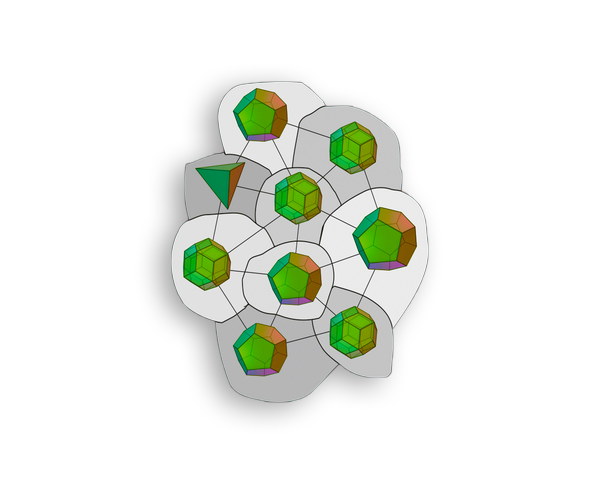
\includegraphics[scale=1.4]{images/spin_networks.png}
    \caption{© Copyright from \emph{L'ordine del tempo} by Carlo Rovelli.}
    %\label{fig:enter-label}
\end{figure}

Within this paradigm, geometric observables undergo quantum fluctuations, shedding light on the intrinsic uncertainty that hence characterizes spacetime at its most fundamental level, as one would expect from a quantum theory of space geometry. 

It is worth highlighting that our current effort has primarily centered on the integration of kinematic constraints derived from gauge and natural symmetries. However, as we progress, it becomes evident that our exploration should extend to include the incorporation of the Hamiltonian constraint, due to the globally hyperbolic structure of spacetime. This additional facet is pivotal as it not only enriches our understanding but also serves as a crucial component in the formulation of spin foams, which are so related to the quantum dynamics of spacetime and should allow to reach an utter viewpoint on the quantum spacetime geometry.\\

We acknowledge that this presentation deviates from historical LQG in several aspects:

\begin{itemize}
\item We embark on a mathematically grounded examination of the main objects of differential geometry that the theory involves, particularly connections and their curvature, shedding light on various aspects crucial for subsequent advancements. This is done along the whole Chapter 1.
\item The BI reduction process, as detailed in Section \ref{BI_red}, is underpinned by a meticulously demonstrated argument grounded in the principles of differential geometry, as discussed in \cite{kobayashi1} and \cite{Orizzonte}: the splitting argument is made on the spacetime, not in space, as it is usually done in the literature. Among its various facets, this argument elucidates a dimensional sensitivity inherent in deriving the Barbero--Immirzi connection. For instance, in four-dimensional spacetimes, such reductions are parameterized by a $\beta\in\R$, distinguishing it as a kinematical quantity distinct from the dynamical Holst parameter $\gamma\in\R\setminus\{0\}$. Moreover, in spacetimes of dimension $3$ or strictly greater than $4$, the parameter turns out to be $\beta=0$, offering intriguing avenues for further mathematical exploration in this direction.
\item In the evolutionary interpretation of Holst theory, the canonical analysis offers a refined approach, yielding boundary equations directly from mathematical principles rather than resorting to ad--hoc definitions. Furthermore, a fresh interpretation of the covariant Cauchy problem emerges with the formalization of Cauchy bubbles and pre--quantum states---see \cite{LN2}.
\item In the implementation of the constraint equations on the quantum space of kinematical states, imposing the gauge and diffeomorphism invariance leads us to invariant states that represent the spatial aspect of the gravitational field. These states are characterized by (possibly knotted) spin networks residing within a separable Hilbert space modeled on lattices. Another noteworthy outcome of our discussion is that, as we delve into the realm of spin knots, the direct relationship with the manifold structure fades away. {Indeed, one can examine what happens to the corresponding functionals when one changes the way links are knotted, resulting in spin knots being insensitive to the knotting of links: they depend only on the abstract lattice. This implies that upon implementing $\Diffeo_*$--invariance, the perceived embedding of the lattice dissipates, leaving behind only abstract lattice structures at the quantum level}.

\item We have introduced operators for holonomies, which are contingent upon the fields $\A^i_a(k)$, as well as momenta operators, which are dependent on the densitized triads $\E^a_i(k)$. Through precise definitions of these operators, the need for postulating commutators is obviated, allowing for straightforward computation within the framework of our model.
  
\end{itemize} 







  
%- Embracing an abstract lattice-only approach (as discussed in LN7), we observe a departure from the traditional emphasis on manifold structure, allowing for a more flexible framework.
  
%- By providing precise definitions for operators governing holonomies and momenta, which depend respectively on connections and densitized triads, we eliminate the need for postulating commutators, thus enabling straightforward computation.

%$$\vdots$$
%Diciamo qui che questa presentazione è diversa da LQG storica: i punti che sono stati approcciati diversamente sono

%\begin{itemize}
   % \item mathematical--founded study of connections wich clarifies many aspects useful in the next steps
    
    %\item BI reduction (C\&P of LN3) the reduction procedure to obtain Barbero-Immirzi connection is dimensional sensitive, as the original Holst dynamics is.

    %\item Canonical analysis in the evolutionary reduction getting boundary equations as mathematically derived, not as a--doc definitions.
    
   % \item Abstract lattice only (C\&P of LN7) "the manifold structure has mainly slipped away"

    %\item We have introduced operators for holonomies, which are contingent upon the connection, although not directly derived from the fields $\A^i_a(k)$, as well as momenta, which are dependent on the densitized triad $\E^a_i(k)$. Through precise definitions of these operators, the need for postulating commutators is obviated, allowing for straightforward computation within the framework of our model.
    
   % We gave operators for holonomies (which depend on the connection, though not directly from the fields $\A^i_a(k)$) and momenta (which depend on the densitized triad $\E^a_i(k)$). Since we defined these operators precisely, we do not need to postulate commutators, we simply can compute them.
%\end{itemize}
As mentioned earlier, we have advanced LQG to the point where we can describe a quantum geometry of spatial leaves of spacetime composed of quantum tetrahedra, whose geometric characteristics are subjected to uncertainty. The next step would be to extend this framework to encompass the entire spacetime, by including consideration of the Hamiltonian constraint. {As a matter of fact, in order to solve the Hamiltonian constraint into our Hilbert quantum space, it is convenient to begin by introducing the area and volume operators. This supports the interpretation of the quantum Hamiltonian operator in terms of their commutators and underscores the fact that geometric observables, such as areas and volumes, are kinematical and remain independent of the Hamiltonian operator, being instead dynamical.}

As a matter of fact, path--quantisation is the prevailing approach that has been pursued, within the LQG community, to reach such a quantum description of spacetime. However, the discussion presented in this thesis suggests that one can see quantisation also in an alternative more algebraic point of view: one could potentially extend the arguments discussed throughout Chapter 3 directly to spacetime, aiming to handle the dynamical physical states of spacetime (so--called spin foams) through a lattice formalism involving the irreducible representations of $\SL(2,\C)$ directly. These representations are infinite--dimensional, given that $\SL(2,\C)$ is a non--compact Lie group. This approach opens up new avenues for exploration within the realm of LQG. %paving the way for a deeper understanding of the quantum nature of spacetime.

Another possible way is to frame the discussion in the context of differential topology. As we have observed throughout our exploration, any relativistic theory, including standard GR, can be viewed as a field theory on a bare manifold. This mathematical setting is well--studied in differential topology and offers a rich framework for theoretical investigations. A proposed approach involves utilizing CW--complexes to delve into the realm of spin foams, such objects living in the natural category of loops' homotopies. Moreover, the \emph{geometric algebra} of Grassmann constitutes a promising and only partially explored framework for setting up the final developments of kinematical LQG discussed in this work, offering a way to making arise the geometry of tetrahedra naturally, instead of recovering and studying it a--posteriori, in the arena of multilinear algebra---see \cite{blake} for Whitehead's book on Grassmann geometric algebra. These alternative perspectives could promise to shed new light on the intricate interplay between geometric structures and quantum phenomena in spacetime.

Despite the four--dimensional nature of our physical spacetime, LQG exhibits a remarkable adaptability to any dimension which is shared by GR. This characteristic prompts an exploration into a $3$--dimensional formulation of LQG, aiming to uncover traits that may shed light on new aspects not readily apparent in the original theory. Moreover, it offers a remarkable laboratory to test ideas of loop quantisation (see Section 9.6 of \cite{pullin2} and Section 9.3.1 of \cite{rov1}). This endeavor should involve delving into the representations of $\Spin(1,2)$ instead, which is infinite dimensional, being isomorphic to $\SL(2,\R)$---as well as $\SL(2,\C)$, whose irreducible representations aim to describe spin foams---along with its $\Spin(2)\cong\mathrm{U}(1)$--reduction, allowing finite--dimensional irreducible representations, being $\mathrm{U}(1)\cong\mathbb{S}^1$ compact, alike to the approach taken for $\mathrm{Spin}(1,3)$ and $\mathrm{Spin}(3)$, along the whole Chapter 2.\\

Concluding, the discussion on the gravitational field revealed a natural quantisation of space geometry that can be studied independently. Here, I followed an original approach by studying the algebra of invariant operators rather than defining individual cases of invariant operators, as in the literature. This approach proved to be interesting because one could use the standard tools built for analyzing algebra representations. For example, one can detect the maximal commuting sub--algebras of the observables' algebra, providing quantum numbers' choices and allowing to compute the quantum behavior of the remaining quantities.

From this perspective, LQG reduces to the choice---at each node---of areas and volumes as compatible quantities, having spin networks as eigenstates, enabling the definition of other invariant operators (such as the other dihedrals) that encompass the quantum aspects of the considered geometry.


%Cosa si può sperare di fare dopo:

%\begin{itemize}
 %   \item C\&P of LN9 per nuova approccio a spinfoams rifacendo tutto con le rappresentazioni infinito dimensionali di $\SL(2,\C)$
  %  \item As we noticed along the way, mathematically speaking, any relativistic theory (and standard GR) is a field theory on a bare manifold, a setting which in mathematics is called differential topology; proposta di approccio a spinfoams con CW--complexes

   % \item Even if the spacetime of our physical world is $4$--dimensional, the theory does adapt to any dimension. It is for this reason that, in conclusion, I will discuss an attempt of a $3$--dimensional formulation of LQG, looking for some traits that can shed light on new aspects that may not be manifest in the original theory.
   % $$\vdots$$
    %Questo involverebe le rappresentazioni (infinito dimensionali) di $\SL(2,\R)$ e le sue $\U(1)$--reduction ($\U(1)\cong\S^1$ compatto, simile a quanto fatto per $\Spin(1,3)$ e $\Spin(3)$)
%\end{itemize}

%\appendix
%\chapter{Albero}
%%\section{Lie Operators for the ground state}

In the final part of this work, we have seen that the quantisation of a gauge theory equivalent to GR leads to a quantum theory of space where the invariant quantum states are represented by superpositions of spin networks, which can be identified as quantum tetrahedra, the observables of this theory corresponding to the geometric properties of these tetrahedra. We have also observed that the algebra of observables is polynomial in the dihedral angles $\Dd_{ij}$, which can be viewed as inner products of Lie operators $(L_i)_a$, regarding them as the fundamental building blocks of such a geometric algebra.

Technically, quantum tetrahedra with generic spins \((j_1, j_2, j_3, j_4)\) imply geometric operators that are endomorphisms of the vector space \(\mathbb{C}^{n_{(j_1)}} \otimes \mathbb{C}^{n_{(j_2)}} \otimes \mathbb{C}^{n_{(j_3)}} \otimes \mathbb{C}^{n_{(j_4)}}\) and the Lie operators reconstruct these by acting Leibniz--like manner on each component of the tensor product through some representation $L_a$ on the correspondent $\C^{n_{(j_i)}}$. Consequently, the dimensions of the matrices are highly sensitive to the values of the spins: the first two simplest examples (except the ground state) are the tetrahedra \((1, \frac{1}{2}, \frac{1}{2}, 1)\) and \((1, 1, 1, 1)\), whose geometric algebras have bases spanned by symmetric matrices of dimensions \(36 \times 36\) and \(81 \times 81\) respectively, and quickly escalating to the case \((\frac{3}{2},\frac{3}{2},\frac{3}{2},\frac{3}{2})\) which has a support of dimension $256$.

Therefore, we opted to exploit invariance to tame the exponential growth in dimension of these matrices, viewing them restricted to the relevant subspace $\Inv(\rho)$, resulting in matrices of dimensions \((2j+1) \times (2j+1)\) at most\footnote{Indeed, unlike the Lie ones, dihedral angles are invariant operators, hence they allow the spin networks space $\Inv(\rho)$, which is of dimension $2$ for the ground state tetrahedron, and they write as $2\times2$ symmetric matrices.}---see Theorem 3.1.3.\\

However, the case of the geometric algebra of the ground state tetrahedron is still manageable in its general version, where its Lie operators can be written as \(16 \times 16\) matrices.
The whole machinery relies on the isomorphism ${\C^{2}}^{\otimes 4}\cong\C^{16}$, that can be cumbersomely written explicitly on the basis and then extend by linearity. For instance
$$\begin{matrix}
    \ket{++++}\in{\C^2}^{\otimes4}&\leftrightarrow&\begin{bmatrix}
    1\\
    0\\
    0\\
    \vdots\\
    0\\
    \vdots\\
    0
\end{bmatrix}\quad\begin{matrix}
    \ket{++++}\\
    \ket{+++-}\\
    \ket{++-+}\\
    \vdots\\
    \ket{+-+-}\\
    \vdots\\
    \ket{----}
\end{matrix}\in\C^{16}
\end{matrix}$$

$$\begin{matrix}
    \ket{+-+-}\in{\C^2}^{\otimes4}&\leftrightarrow&\begin{bmatrix}
    0\\
    0\\
    0\\
    \vdots\\
    1\\
    \vdots\\
    0
\end{bmatrix}\quad\begin{matrix}
    \ket{++++}\\
    \ket{+++-}\\
    \ket{++-+}\\
    \vdots\\
    \ket{+-+-}\\
    \vdots\\
    \ket{----}
\end{matrix}\in\C^{16}
\end{matrix}$$
$$\vdots$$
$$\begin{matrix}
    \ket{----}\in{\C^2}^{\otimes4}&\leftrightarrow&\begin{bmatrix}
    0\\
    0\\
    0\\
    \vdots\\
    0\\
    \vdots\\
    1
\end{bmatrix}\quad\begin{matrix}
    \ket{++++}\\
    \ket{+++-}\\
    \ket{++-+}\\
    \vdots\\
    \ket{+-+-}\\
    \vdots\\
    \ket{----}
\end{matrix}\in\C^{16}
\end{matrix}$$

%$$\text{e.g.}\quad\ket{+-+-}\in{\C^{2}}^{\otimes 4}\cong\C^{16}\quad\text{reads as}$$
%$$\begin{bmatrix}
 %   0\\
  %  0\\
   % 0\\
    %\vdots\\
    %1\\
    %\vdots\\
    %0
%\end{bmatrix}\quad\begin{matrix}
 %   \ket{++++}\\
  %  \ket{+++-}\\
   % \ket{++-+}\\
    %\vdots\\
    %\ket{+-+-}\\
    %\vdots\\
    %\ket{----}
%\end{matrix}$$

%Now you can compute the matrices $(L_i)_a\in\C^{16\times 16}\Rightarrow(L_i)_a\ket{\pm\pm\pm\pm}\in\C^{16}$ such that---for indices $a,i=1,2,3$ they are $9$ matrices
%$$\begin{bmatrix}
 %   (L_i)_a\ket{++++}&(L_i)_a\ket{+++-}&\hdots&(L_i)_a\ket{----}
%\end{bmatrix}\in\C^{16\times 16}$$
%through (\ref{tau_i}), by extending Leibnitz--like in each component.

%\newpage
%$$\begin{bmatrix}
 %   1\\
  %  0\\
   % 0\\
    %0\\
 %   0\\
  %  0\\
   % 0\\
    %0\\
 %   0\\
  %  0\\
   % 0\\
    %0\\
 %   0\\
  %  0\\
   % 0\\
    %0\\
    %0\\
%\end{bmatrix}=\ket{++++}$$

%$$\vdots$$
%$$\mathfrak{geo}=\bigg\{X\in\mathfrak{gl}_3(\R)\,\bigg|\,X^{-1}+X\in\mathfrak{so}(3)\bigg\}$$
%if $\Geo$ were a Lie group, the above would be its Lie algebra. Actually it is a homogenoeus space, i.e. it has smooth structure supporting the action of $\SO(3)$ through its diffeomorphisms, i.e. there exists a group homomorphism (a representation) $\rho:\SO(3)\to\Diffeo(\Geo)$.\\

Let us now compute Lie operators---for each $a=1,2,3,4$ and $i=1,2,3$.

Recall the Kronecker product, being defined for two vectors $x,y\in\C^n$ as $(x\otimes y)_{ij}=x^iy^j$, while for two matrices $X,Y\in\C^{n\times n}$ results $(X\otimes Y)_{ij}=X_{ij}Y$. This way, we can compute the twelve Lie matrices 

\begin{align*}
    (L_1)_a&=\tau_a\otimes\1_2\otimes\1_2\otimes\1_2\\
    (L_2)_a&=\1_2\otimes\tau_a\otimes\1_2\otimes\1_2\\
    (L_3)_a&=\1_2\otimes\1_2\otimes\tau_a\otimes\1_2\\
    (L_0)_a&=-\bigg((L_1)_a+(L_2)_a+(L_3)_a\bigg)
\end{align*}
Since $\1_1\otimes\1_2=\1_4$, we have
\begin{align*}
    (L_1)_1&=-\frac{i}{2}\begin{bmatrix}
    0&1\\
    1&0
\end{bmatrix}\otimes\begin{bmatrix}
    1&0\\
    0&1
\end{bmatrix}\otimes\1_4=-\frac{i}{2}\begin{bmatrix}
    0&0&1&0\\
    0&0&0&1\\
    1&0&0&0\\
    0&1&0&0
\end{bmatrix}\otimes\begin{bmatrix}
    1&0&0&0\\
    0&1&0&0\\
    0&0&1&0\\
    0&0&0&1
\end{bmatrix}\\
&=-\frac{i}{2}\begin{bmatrix}
    \mathbb{0}_4&\mathbb{0}_4&\1_4&\mathbb{0}_4\\
    \mathbb{0}_4&\mathbb{0}_4&\mathbb{0}_4&\1_4\\
    \1_4&\mathbb{0}_4&\mathbb{0}_4&\mathbb{0}_4\\
    \mathbb{0}_4&\1_4&\mathbb{0}_4&\mathbb{0}_4
\end{bmatrix}
\end{align*}

\,\newline
Analogously we can compute
\begin{align*}
    (L_1)_2&=\tau_2\otimes\1_2\otimes\1_2\otimes\1_2=\frac{1}{2}\begin{bmatrix}
        \0_4&\0_4&-\1_4&\0_4\\
        \0_4&\0_4&\0_4&-\1_4\\
        \1_4&\0_4&\0_4&\0_4\\
        \0_4&\1_4&\0_4&\0_4
    \end{bmatrix}
\end{align*}

\begin{align*}
    (L_1)_3&=\tau_3\otimes\1_2\otimes\1_2\otimes\1_2=-\frac{i}{2}\begin{bmatrix}
        \1_4&\0_4&\0_4&\0_4\\
        \0_4&\1_4&\0_4&\0_4\\
        \0_4&\0_4&-\1_4&\0_4\\
        \0_4&\0_4&\0_4&-\1_4
    \end{bmatrix}
\end{align*}
\begin{align*}
    (L_2)_1&=\1_2\otimes\tau_1\otimes\1_2\otimes\1_2=-\frac{i}{2}\begin{bmatrix}
        \0_4&\1_4&\0_4&\0_4\\
        \1_4&\0_4&\0_4&\0_4\\
        \0_4&\0_4&\0_4&\1_4\\
        \0_4&\0_4&\1_4&\0_4
    \end{bmatrix}
\end{align*}
\begin{align*}
    (L_2)_2&=\1_2\otimes\tau_2\otimes\1_2\otimes\1_2=\frac{1}{2}\begin{bmatrix}
        \0_4&-\1_4&\0_4&\0_4\\
        \1_4&\0_4&\0_4&\0_4\\
        \0_4&\0_4&\0_4&-\1_4\\
        \0_4&\0_4&\1_4&\0_4
    \end{bmatrix}
\end{align*}

\begin{align*}
    (L_2)_3&=\1_2\otimes\tau_3\otimes\1_2\otimes\1_2=-\frac{i}{2}\begin{bmatrix}
        \1_4&\0_4&\0_4&\0_4\\
        \0_4&-\1_4&\0_4&\0_4\\
        \0_4&\0_4&\1_4&\0_4\\
        \0_4&\0_4&\0_4&-\1_4
    \end{bmatrix}
\end{align*}



\begin{align*}
    (L_3)_1&=\1_4\otimes-\frac{i}{2}\begin{bmatrix}
        0&1\\
        1&0
    \end{bmatrix}\otimes\1_2=-\frac{i}{2}\1_4\otimes\begin{bmatrix}
        \0_2&\1_2\\
        \1_2&\0_2
    \end{bmatrix}\\
    &=-\frac{i}{2}\begin{bmatrix}
        \0_2&\1_2&\0_2&\0_2&\0_2&\0_2&\0_2&\0_2\\
        \1_2&\0_2&\0_2&\0_2&\0_2&\0_2&\0_2&\0_2\\
        \0_2&\0_2&\0_2&\1_2&\0_2&\0_2&\0_2&\0_2\\
        \0_2&\0_2&\1_2&\0_2&\0_2&\0_2&\0_2&\0_2\\
        \0_2&\0_2&\0_2&\0_2&\0_2&\1_2&\0_2&\0_2\\
        \0_2&\0_2&\0_2&\0_2&\1_2&\0_2&\0_2&\0_2\\
        \0_2&\0_2&\0_2&\0_2&\0_2&\0_2&\0_2&\1_2\\
        \0_2&\0_2&\0_2&\0_2&\0_2&\0_2&\1_2&\0_2\\
    \end{bmatrix}
\end{align*}

\begin{align*}
    (L_3)_2&=\1_4\otimes-\frac{i}{2}\begin{bmatrix}
        0&-i\\
        i&0
    \end{bmatrix}\otimes\1_2=\frac{1}{2}\1_4\otimes\begin{bmatrix}
        \0_2&-\1_2\\
        \1_2&\0_2
    \end{bmatrix}\\
    &=\frac{1}{2}\begin{bmatrix}
        \0_2&-\1_2&\0_2&\0_2&\0_2&\0_2&\0_2&\0_2\\
        \1_2&\0_2&\0_2&\0_2&\0_2&\0_2&\0_2&\0_2\\
        \0_2&\0_2&\0_2&-\1_2&\0_2&\0_2&\0_2&\0_2\\
        \0_2&\0_2&\1_2&\0_2&\0_2&\0_2&\0_2&\0_2\\
        \0_2&\0_2&\0_2&\0_2&\0_2&-\1_2&\0_2&\0_2\\
        \0_2&\0_2&\0_2&\0_2&\1_2&\0_2&\0_2&\0_2\\
        \0_2&\0_2&\0_2&\0_2&\0_2&\0_2&\0_2&-\1_2\\
        \0_2&\0_2&\0_2&\0_2&\0_2&\0_2&\1_2&\0_2\\
    \end{bmatrix}
\end{align*}


\begin{align*}
    (L_3)_3&=\1_4\otimes-\frac{i}{2}\begin{bmatrix}
        1&0\\
        0&-1
    \end{bmatrix}\otimes\1_2=-\frac{i}{2}\1_4\otimes\begin{bmatrix}
        \1_2&\0_2\\
        \0_2&-\1_2
    \end{bmatrix}\\
    &=-\frac{i}{2}\begin{bmatrix}
        \1_2&\0_2&\0_2&\0_2&\0_2&\0_2&\0_2&\0_2\\
        \0_2&-\1_2&\0_2&\0_2&\0_2&\0_2&\0_2&\0_2\\
        \0_2&\0_2&\1_2&\0_2&\0_2&\0_2&\0_2&\0_2\\
        \0_2&\0_2&\0_2&-\1_2&\0_2&\0_2&\0_2&\0_2\\
        \0_2&\0_2&\0_2&\0_2&\1_2&\0_2&\0_2&\0_2\\
        \0_2&\0_2&\0_2&\0_2&\0_2&-\1_2&\0_2&\0_2\\
        \0_2&\0_2&\0_2&\0_2&\0_2&\0_2&\1_2&\0_2\\
        \0_2&\0_2&\0_2&\0_2&\0_2&\0_2&\0_2&-\1_2\\
    \end{bmatrix}
\end{align*}

Once all Lie matrices are computed, we can use them to reconstruct each dihedral operator of the ground state through $\Dd_{ij}=(L_i)_a\delta^{ab}(L_j)_b$. For instance

$$\Dd_{12}=\frac{1}{4}\begin{bmatrix}
    -\1_4&\0_4&\0_4&\0_4\\
    \0_4&\1_4&-2\1_4&\0_4\\
    \0_4&-2\1_4&\1_4&\0_4\\
    \0_4&\0_4&\0_4&-\1_4
\end{bmatrix}\quad\text{and}\quad\Dd_{33}=-\frac{3}{4}\1_{16}$$



%\chapter{Barca}
%%\section{Loop Quantum Gravity in (1,2)--signature}

LQG in three dimensions could be interesting, even just from a mathematical viewpoint. Moreover, it offers a remarkable laboratory to test ideas of loop quantisation---see Section 9.6 of \cite{pullin2} and Section 9.3.1 of \cite{rov1}.\\

The starting point will be a Holst--like theory on a 3--dimensional spacetime $\M^{1,2}$; the Lagrangian must be a $3$--form on $\J^1\Ci$ with $\Ci=\mathcal{F}(P)\times_{\M^{1,2}}\Con(P)$, for a principal $\Spin(1,2)$--bundle $P\xrightarrow{\pi}\M^{1,2}$ not depending on any Holst parameter! i.e., up to physical constants, it is

$$\mathbf{L}=R^{ij}\wedge e^k\,\epsilon_{ijk}\textcolor{gray}{-\frac{\Lambda}{6}e^i\wedge e^j\wedge e^k\,\epsilon_{ijk}}$$
which produces a variation
\begin{align*}
    \delta\mathbf{L}&=\epsilon_{ijk}\Biggl(\delta R^{ij}\wedge e^k+R^{ij}\wedge\delta e^k-\tiny{\frac{\Lambda}{6}}\bigg(\delta e^i\wedge e^j\wedge e^k+e^i\wedge\delta e^j\wedge e^k+e^i\wedge e^j\wedge\delta e^k\bigg)\Biggl)\\
    &=\epsilon_{ijk}\left(\nablaw\delta\omega^{ij}\wedge e^k+R^{ij}\wedge\delta e^k+\frac{\Lambda}{2}\, e^i\wedge e^j \wedge\delta e^k\right)\\
    &=\epsilon_{ijk}\left(\left(R^{ij}+\frac{\Lambda}{2}\,e^i\wedge e^j\right)\wedge\delta e^k-\nablaw e^k\wedge\delta\omega^{ij}\right)
\end{align*}
and $\delta\mathbf{S}=0$ implies by Theorem \ref{least_action} field equations
\begin{equation}
    \begin{cases}
    R^{ij}\textcolor{gray}{+\frac{\Lambda}{2}\,e^i\wedge e^j}=0\\
    \nablaw e^k=0
    \end{cases}
\end{equation}
Even if they characterise spacetimes in dimension $3$ to be flat, the theory is nevertheless non--trivial if the space--like surfaces have non--trivial global topology.\\

At this stage we could discuss either the (possibly infinite--dimensional) irreducible representations of $\Spin(1,2)\cong\SL(2,\R)$, in order to get \emph{spin foams} for a $3$--dimensional spacetime, or the finite--dimensional representations of $\Spin(2)\cong\U(1)$ to describe spin networks of a $2$--dimensional space.

The theory of representations of \(\mathfrak{sl}(2,\mathbb{R})\) is well established. Considering that \(\U(1) \subseteq \SL(2,\mathbb{R})\), any representation of \(\SL(2,\mathbb{R})\) must also be a representation of \(\U(1)\). The representations of \(\U(1)\), being compact, are classified in a manner similar to those of \(\SU(2)\).

In LQG literature, there is an ad--hoc prescription to construct spin foams in the case of \(\SL(2,\mathbb{C})\) along similar lines. Investigating the connections between these two approaches can be interesting.

%\subsection{\texorpdfstring{$\Spin(2)$}{a}--reduction of \texorpdfstring{$\Spin(1,2)$}{a}--bundles}

%$\Spin(2)\cong\U(1)\cong\SO(2)\cong\S^1$ and $\Spin(1,2)\cong\SL(2,\R)$. Qui possiamo implementare le rappresentazioni (infinito dimensionali) di $\SL(2,\R)$ per ottenre spinfoams in segnatura $(1,2)$, oppure possiamo implementare le rappresentazioni (finito dimensionali) di $\U(1)$ per descrivere spin--networks in segnatura $(1,2)$.   
%$$\vdots$$

%$$\L\left(\e,j^1\A,j^1\kappa\right)=\frac{1}{\boldsymbol{\kappa}}\bigg(2\nabla\kappa^i\wedge e^k\epsilon_{i0k}+\epsilon^{ij}_kF^k\wedge e^k\,\epsilon_{ijk}+2\kappa^i\wedge\kappa^j\wedge\kappa^k\,\epsilon_{ijk}\bigg)$$

%$$F^k_{ab}=\der_a\A_b^k-\der_b\A_a^k-\epsilon_{ij}^k\A_a^i\A_b^j$$

%$$p^{ab}_k=\frac{1}{\boldsymbol{\kappa}}\epsilon^{ij}_k\epsilon_{ijk}\,e^k\,\epsilon^{ab}$$

%$$\vdots$$




\chapter*{Appendix A: Lie Operators for the ground state}
\markboth{\MakeUppercase{Lie Operators for the ground state}}{}
\addcontentsline{toc}{chapter}{Appendix A}
%\section{Lie Operators for the ground state}

In the final part of this work, we have seen that the quantisation of a gauge theory equivalent to GR leads to a quantum theory of space where the invariant quantum states are represented by superpositions of spin networks, which can be identified as quantum tetrahedra, the observables of this theory corresponding to the geometric properties of these tetrahedra. We have also observed that the algebra of observables is polynomial in the dihedral angles $\Dd_{ij}$, which can be viewed as inner products of Lie operators $(L_i)_a$, regarding them as the fundamental building blocks of such a geometric algebra.

Technically, quantum tetrahedra with generic spins \((j_1, j_2, j_3, j_4)\) imply geometric operators that are endomorphisms of the vector space \(\mathbb{C}^{n_{(j_1)}} \otimes \mathbb{C}^{n_{(j_2)}} \otimes \mathbb{C}^{n_{(j_3)}} \otimes \mathbb{C}^{n_{(j_4)}}\) and the Lie operators reconstruct these by acting Leibniz--like manner on each component of the tensor product through some representation $L_a$ on the correspondent $\C^{n_{(j_i)}}$. Consequently, the dimensions of the matrices are highly sensitive to the values of the spins: the first two simplest examples (except the ground state) are the tetrahedra \((1, \frac{1}{2}, \frac{1}{2}, 1)\) and \((1, 1, 1, 1)\), whose geometric algebras have bases spanned by symmetric matrices of dimensions \(36 \times 36\) and \(81 \times 81\) respectively, and quickly escalating to the case \((\frac{3}{2},\frac{3}{2},\frac{3}{2},\frac{3}{2})\) which has a support of dimension $256$.

Therefore, we opted to exploit invariance to tame the exponential growth in dimension of these matrices, viewing them restricted to the relevant subspace $\Inv(\rho)$, resulting in matrices of dimensions \((2j+1) \times (2j+1)\) at most\footnote{Indeed, unlike the Lie ones, dihedral angles are invariant operators, hence they allow the spin networks space $\Inv(\rho)$, which is of dimension $2$ for the ground state tetrahedron, and they write as $2\times2$ symmetric matrices.}---see Theorem 3.1.3.\\

However, the case of the geometric algebra of the ground state tetrahedron is still manageable in its general version, where its Lie operators can be written as \(16 \times 16\) matrices.
The whole machinery relies on the isomorphism ${\C^{2}}^{\otimes 4}\cong\C^{16}$, that can be cumbersomely written explicitly on the basis and then extend by linearity. For instance
$$\begin{matrix}
    \ket{++++}\in{\C^2}^{\otimes4}&\leftrightarrow&\begin{bmatrix}
    1\\
    0\\
    0\\
    \vdots\\
    0\\
    \vdots\\
    0
\end{bmatrix}\quad\begin{matrix}
    \ket{++++}\\
    \ket{+++-}\\
    \ket{++-+}\\
    \vdots\\
    \ket{+-+-}\\
    \vdots\\
    \ket{----}
\end{matrix}\in\C^{16}
\end{matrix}$$

$$\begin{matrix}
    \ket{+-+-}\in{\C^2}^{\otimes4}&\leftrightarrow&\begin{bmatrix}
    0\\
    0\\
    0\\
    \vdots\\
    1\\
    \vdots\\
    0
\end{bmatrix}\quad\begin{matrix}
    \ket{++++}\\
    \ket{+++-}\\
    \ket{++-+}\\
    \vdots\\
    \ket{+-+-}\\
    \vdots\\
    \ket{----}
\end{matrix}\in\C^{16}
\end{matrix}$$
$$\vdots$$
$$\begin{matrix}
    \ket{----}\in{\C^2}^{\otimes4}&\leftrightarrow&\begin{bmatrix}
    0\\
    0\\
    0\\
    \vdots\\
    0\\
    \vdots\\
    1
\end{bmatrix}\quad\begin{matrix}
    \ket{++++}\\
    \ket{+++-}\\
    \ket{++-+}\\
    \vdots\\
    \ket{+-+-}\\
    \vdots\\
    \ket{----}
\end{matrix}\in\C^{16}
\end{matrix}$$

%$$\text{e.g.}\quad\ket{+-+-}\in{\C^{2}}^{\otimes 4}\cong\C^{16}\quad\text{reads as}$$
%$$\begin{bmatrix}
 %   0\\
  %  0\\
   % 0\\
    %\vdots\\
    %1\\
    %\vdots\\
    %0
%\end{bmatrix}\quad\begin{matrix}
 %   \ket{++++}\\
  %  \ket{+++-}\\
   % \ket{++-+}\\
    %\vdots\\
    %\ket{+-+-}\\
    %\vdots\\
    %\ket{----}
%\end{matrix}$$

%Now you can compute the matrices $(L_i)_a\in\C^{16\times 16}\Rightarrow(L_i)_a\ket{\pm\pm\pm\pm}\in\C^{16}$ such that---for indices $a,i=1,2,3$ they are $9$ matrices
%$$\begin{bmatrix}
 %   (L_i)_a\ket{++++}&(L_i)_a\ket{+++-}&\hdots&(L_i)_a\ket{----}
%\end{bmatrix}\in\C^{16\times 16}$$
%through (\ref{tau_i}), by extending Leibnitz--like in each component.

%\newpage
%$$\begin{bmatrix}
 %   1\\
  %  0\\
   % 0\\
    %0\\
 %   0\\
  %  0\\
   % 0\\
    %0\\
 %   0\\
  %  0\\
   % 0\\
    %0\\
 %   0\\
  %  0\\
   % 0\\
    %0\\
    %0\\
%\end{bmatrix}=\ket{++++}$$

%$$\vdots$$
%$$\mathfrak{geo}=\bigg\{X\in\mathfrak{gl}_3(\R)\,\bigg|\,X^{-1}+X\in\mathfrak{so}(3)\bigg\}$$
%if $\Geo$ were a Lie group, the above would be its Lie algebra. Actually it is a homogenoeus space, i.e. it has smooth structure supporting the action of $\SO(3)$ through its diffeomorphisms, i.e. there exists a group homomorphism (a representation) $\rho:\SO(3)\to\Diffeo(\Geo)$.\\

Let us now compute Lie operators---for each $a=1,2,3,4$ and $i=1,2,3$.

Recall the Kronecker product, being defined for two vectors $x,y\in\C^n$ as $(x\otimes y)_{ij}=x^iy^j$, while for two matrices $X,Y\in\C^{n\times n}$ results $(X\otimes Y)_{ij}=X_{ij}Y$. This way, we can compute the twelve Lie matrices 

\begin{align*}
    (L_1)_a&=\tau_a\otimes\1_2\otimes\1_2\otimes\1_2\\
    (L_2)_a&=\1_2\otimes\tau_a\otimes\1_2\otimes\1_2\\
    (L_3)_a&=\1_2\otimes\1_2\otimes\tau_a\otimes\1_2\\
    (L_0)_a&=-\bigg((L_1)_a+(L_2)_a+(L_3)_a\bigg)
\end{align*}
Since $\1_1\otimes\1_2=\1_4$, we have
\begin{align*}
    (L_1)_1&=-\frac{i}{2}\begin{bmatrix}
    0&1\\
    1&0
\end{bmatrix}\otimes\begin{bmatrix}
    1&0\\
    0&1
\end{bmatrix}\otimes\1_4=-\frac{i}{2}\begin{bmatrix}
    0&0&1&0\\
    0&0&0&1\\
    1&0&0&0\\
    0&1&0&0
\end{bmatrix}\otimes\begin{bmatrix}
    1&0&0&0\\
    0&1&0&0\\
    0&0&1&0\\
    0&0&0&1
\end{bmatrix}\\
&=-\frac{i}{2}\begin{bmatrix}
    \mathbb{0}_4&\mathbb{0}_4&\1_4&\mathbb{0}_4\\
    \mathbb{0}_4&\mathbb{0}_4&\mathbb{0}_4&\1_4\\
    \1_4&\mathbb{0}_4&\mathbb{0}_4&\mathbb{0}_4\\
    \mathbb{0}_4&\1_4&\mathbb{0}_4&\mathbb{0}_4
\end{bmatrix}
\end{align*}

\,\newline
Analogously we can compute
\begin{align*}
    (L_1)_2&=\tau_2\otimes\1_2\otimes\1_2\otimes\1_2=\frac{1}{2}\begin{bmatrix}
        \0_4&\0_4&-\1_4&\0_4\\
        \0_4&\0_4&\0_4&-\1_4\\
        \1_4&\0_4&\0_4&\0_4\\
        \0_4&\1_4&\0_4&\0_4
    \end{bmatrix}
\end{align*}

\begin{align*}
    (L_1)_3&=\tau_3\otimes\1_2\otimes\1_2\otimes\1_2=-\frac{i}{2}\begin{bmatrix}
        \1_4&\0_4&\0_4&\0_4\\
        \0_4&\1_4&\0_4&\0_4\\
        \0_4&\0_4&-\1_4&\0_4\\
        \0_4&\0_4&\0_4&-\1_4
    \end{bmatrix}
\end{align*}
\begin{align*}
    (L_2)_1&=\1_2\otimes\tau_1\otimes\1_2\otimes\1_2=-\frac{i}{2}\begin{bmatrix}
        \0_4&\1_4&\0_4&\0_4\\
        \1_4&\0_4&\0_4&\0_4\\
        \0_4&\0_4&\0_4&\1_4\\
        \0_4&\0_4&\1_4&\0_4
    \end{bmatrix}
\end{align*}
\begin{align*}
    (L_2)_2&=\1_2\otimes\tau_2\otimes\1_2\otimes\1_2=\frac{1}{2}\begin{bmatrix}
        \0_4&-\1_4&\0_4&\0_4\\
        \1_4&\0_4&\0_4&\0_4\\
        \0_4&\0_4&\0_4&-\1_4\\
        \0_4&\0_4&\1_4&\0_4
    \end{bmatrix}
\end{align*}

\begin{align*}
    (L_2)_3&=\1_2\otimes\tau_3\otimes\1_2\otimes\1_2=-\frac{i}{2}\begin{bmatrix}
        \1_4&\0_4&\0_4&\0_4\\
        \0_4&-\1_4&\0_4&\0_4\\
        \0_4&\0_4&\1_4&\0_4\\
        \0_4&\0_4&\0_4&-\1_4
    \end{bmatrix}
\end{align*}



\begin{align*}
    (L_3)_1&=\1_4\otimes-\frac{i}{2}\begin{bmatrix}
        0&1\\
        1&0
    \end{bmatrix}\otimes\1_2=-\frac{i}{2}\1_4\otimes\begin{bmatrix}
        \0_2&\1_2\\
        \1_2&\0_2
    \end{bmatrix}\\
    &=-\frac{i}{2}\begin{bmatrix}
        \0_2&\1_2&\0_2&\0_2&\0_2&\0_2&\0_2&\0_2\\
        \1_2&\0_2&\0_2&\0_2&\0_2&\0_2&\0_2&\0_2\\
        \0_2&\0_2&\0_2&\1_2&\0_2&\0_2&\0_2&\0_2\\
        \0_2&\0_2&\1_2&\0_2&\0_2&\0_2&\0_2&\0_2\\
        \0_2&\0_2&\0_2&\0_2&\0_2&\1_2&\0_2&\0_2\\
        \0_2&\0_2&\0_2&\0_2&\1_2&\0_2&\0_2&\0_2\\
        \0_2&\0_2&\0_2&\0_2&\0_2&\0_2&\0_2&\1_2\\
        \0_2&\0_2&\0_2&\0_2&\0_2&\0_2&\1_2&\0_2\\
    \end{bmatrix}
\end{align*}

\begin{align*}
    (L_3)_2&=\1_4\otimes-\frac{i}{2}\begin{bmatrix}
        0&-i\\
        i&0
    \end{bmatrix}\otimes\1_2=\frac{1}{2}\1_4\otimes\begin{bmatrix}
        \0_2&-\1_2\\
        \1_2&\0_2
    \end{bmatrix}\\
    &=\frac{1}{2}\begin{bmatrix}
        \0_2&-\1_2&\0_2&\0_2&\0_2&\0_2&\0_2&\0_2\\
        \1_2&\0_2&\0_2&\0_2&\0_2&\0_2&\0_2&\0_2\\
        \0_2&\0_2&\0_2&-\1_2&\0_2&\0_2&\0_2&\0_2\\
        \0_2&\0_2&\1_2&\0_2&\0_2&\0_2&\0_2&\0_2\\
        \0_2&\0_2&\0_2&\0_2&\0_2&-\1_2&\0_2&\0_2\\
        \0_2&\0_2&\0_2&\0_2&\1_2&\0_2&\0_2&\0_2\\
        \0_2&\0_2&\0_2&\0_2&\0_2&\0_2&\0_2&-\1_2\\
        \0_2&\0_2&\0_2&\0_2&\0_2&\0_2&\1_2&\0_2\\
    \end{bmatrix}
\end{align*}


\begin{align*}
    (L_3)_3&=\1_4\otimes-\frac{i}{2}\begin{bmatrix}
        1&0\\
        0&-1
    \end{bmatrix}\otimes\1_2=-\frac{i}{2}\1_4\otimes\begin{bmatrix}
        \1_2&\0_2\\
        \0_2&-\1_2
    \end{bmatrix}\\
    &=-\frac{i}{2}\begin{bmatrix}
        \1_2&\0_2&\0_2&\0_2&\0_2&\0_2&\0_2&\0_2\\
        \0_2&-\1_2&\0_2&\0_2&\0_2&\0_2&\0_2&\0_2\\
        \0_2&\0_2&\1_2&\0_2&\0_2&\0_2&\0_2&\0_2\\
        \0_2&\0_2&\0_2&-\1_2&\0_2&\0_2&\0_2&\0_2\\
        \0_2&\0_2&\0_2&\0_2&\1_2&\0_2&\0_2&\0_2\\
        \0_2&\0_2&\0_2&\0_2&\0_2&-\1_2&\0_2&\0_2\\
        \0_2&\0_2&\0_2&\0_2&\0_2&\0_2&\1_2&\0_2\\
        \0_2&\0_2&\0_2&\0_2&\0_2&\0_2&\0_2&-\1_2\\
    \end{bmatrix}
\end{align*}

Once all Lie matrices are computed, we can use them to reconstruct each dihedral operator of the ground state through $\Dd_{ij}=(L_i)_a\delta^{ab}(L_j)_b$. For instance

$$\Dd_{12}=\frac{1}{4}\begin{bmatrix}
    -\1_4&\0_4&\0_4&\0_4\\
    \0_4&\1_4&-2\1_4&\0_4\\
    \0_4&-2\1_4&\1_4&\0_4\\
    \0_4&\0_4&\0_4&-\1_4
\end{bmatrix}\quad\text{and}\quad\Dd_{33}=-\frac{3}{4}\1_{16}$$




\chapter*{Appendix B: Steps to Loop Quantum Gravity in (1,2) signature}
\markboth{\MakeUppercase{Loop Quantum Gravity in (1,2) signature}}{}
\addcontentsline{toc}{chapter}{Appendix B}
%\section{Loop Quantum Gravity in (1,2)--signature}

LQG in three dimensions could be interesting, even just from a mathematical viewpoint. Moreover, it offers a remarkable laboratory to test ideas of loop quantisation---see Section 9.6 of \cite{pullin2} and Section 9.3.1 of \cite{rov1}.\\

The starting point will be a Holst--like theory on a 3--dimensional spacetime $\M^{1,2}$; the Lagrangian must be a $3$--form on $\J^1\Ci$ with $\Ci=\mathcal{F}(P)\times_{\M^{1,2}}\Con(P)$, for a principal $\Spin(1,2)$--bundle $P\xrightarrow{\pi}\M^{1,2}$ not depending on any Holst parameter! i.e., up to physical constants, it is

$$\mathbf{L}=R^{ij}\wedge e^k\,\epsilon_{ijk}\textcolor{gray}{-\frac{\Lambda}{6}e^i\wedge e^j\wedge e^k\,\epsilon_{ijk}}$$
which produces a variation
\begin{align*}
    \delta\mathbf{L}&=\epsilon_{ijk}\Biggl(\delta R^{ij}\wedge e^k+R^{ij}\wedge\delta e^k-\tiny{\frac{\Lambda}{6}}\bigg(\delta e^i\wedge e^j\wedge e^k+e^i\wedge\delta e^j\wedge e^k+e^i\wedge e^j\wedge\delta e^k\bigg)\Biggl)\\
    &=\epsilon_{ijk}\left(\nablaw\delta\omega^{ij}\wedge e^k+R^{ij}\wedge\delta e^k+\frac{\Lambda}{2}\, e^i\wedge e^j \wedge\delta e^k\right)\\
    &=\epsilon_{ijk}\left(\left(R^{ij}+\frac{\Lambda}{2}\,e^i\wedge e^j\right)\wedge\delta e^k-\nablaw e^k\wedge\delta\omega^{ij}\right)
\end{align*}
and $\delta\mathbf{S}=0$ implies by Theorem \ref{least_action} field equations
\begin{equation}
    \begin{cases}
    R^{ij}\textcolor{gray}{+\frac{\Lambda}{2}\,e^i\wedge e^j}=0\\
    \nablaw e^k=0
    \end{cases}
\end{equation}
Even if they characterise spacetimes in dimension $3$ to be flat, the theory is nevertheless non--trivial if the space--like surfaces have non--trivial global topology.\\

At this stage we could discuss either the (possibly infinite--dimensional) irreducible representations of $\Spin(1,2)\cong\SL(2,\R)$, in order to get \emph{spin foams} for a $3$--dimensional spacetime, or the finite--dimensional representations of $\Spin(2)\cong\U(1)$ to describe spin networks of a $2$--dimensional space.

The theory of representations of \(\mathfrak{sl}(2,\mathbb{R})\) is well established. Considering that \(\U(1) \subseteq \SL(2,\mathbb{R})\), any representation of \(\SL(2,\mathbb{R})\) must also be a representation of \(\U(1)\). The representations of \(\U(1)\), being compact, are classified in a manner similar to those of \(\SU(2)\).

In LQG literature, there is an ad--hoc prescription to construct spin foams in the case of \(\SL(2,\mathbb{C})\) along similar lines. Investigating the connections between these two approaches can be interesting.

%\subsection{\texorpdfstring{$\Spin(2)$}{a}--reduction of \texorpdfstring{$\Spin(1,2)$}{a}--bundles}

%$\Spin(2)\cong\U(1)\cong\SO(2)\cong\S^1$ and $\Spin(1,2)\cong\SL(2,\R)$. Qui possiamo implementare le rappresentazioni (infinito dimensionali) di $\SL(2,\R)$ per ottenre spinfoams in segnatura $(1,2)$, oppure possiamo implementare le rappresentazioni (finito dimensionali) di $\U(1)$ per descrivere spin--networks in segnatura $(1,2)$.   
%$$\vdots$$

%$$\L\left(\e,j^1\A,j^1\kappa\right)=\frac{1}{\boldsymbol{\kappa}}\bigg(2\nabla\kappa^i\wedge e^k\epsilon_{i0k}+\epsilon^{ij}_kF^k\wedge e^k\,\epsilon_{ijk}+2\kappa^i\wedge\kappa^j\wedge\kappa^k\,\epsilon_{ijk}\bigg)$$

%$$F^k_{ab}=\der_a\A_b^k-\der_b\A_a^k-\epsilon_{ij}^k\A_a^i\A_b^j$$

%$$p^{ab}_k=\frac{1}{\boldsymbol{\kappa}}\epsilon^{ij}_k\epsilon_{ijk}\,e^k\,\epsilon^{ab}$$

%$$\vdots$$




\backmatter
\printbibliography
\addcontentsline{toc}{chapter}{References}

%\listoffigures
%\addcontentsline{toc}{chapter}{List of Figures}

%\listoftables
%\addcontentsline{toc}{chapter}{List of Tables}

\printindex
\addcontentsline{toc}{chapter}{Index}



\end{document}